% =====================================================================
%  main.tex —— 汇总文件（Lead 独占）
%  寺杣友秀《コンツェビッチによるウィッテン予想の解決》中文译注本
%  编译：xelatex main.tex（连续两遍）
% =====================================================================
% =====================================================================
%  preamble.tex —— 导言区（Lead 独占；译者只读，不得修改）
%  寺杣友秀《コンツェビッチによるウィッテン予想の解決》
%  （上智大学数学講究録 No.40, 1997）中文译注本 · XeLaTeX 编译
% =====================================================================
\documentclass[11pt,a4paper]{article}

\usepackage[UTF8]{ctex}
\usepackage{amsmath,amssymb,amsthm,mathtools}
\usepackage{mathrsfs}
\usepackage{bm}
\usepackage{graphicx}
\usepackage{tikz}
\usepackage{tikz-cd}
\usepackage[a4paper,left=2.5cm,right=2.5cm,top=2.7cm,bottom=2.8cm]{geometry}
\usepackage[dvipsnames]{xcolor}
\usepackage{enumitem}
\usepackage{booktabs}
\usepackage{array}
\usepackage{multicol}
\usepackage{fancyhdr}
\usepackage{caption}
\usepackage{titlesec}
\usepackage[hidelinks,unicode]{hyperref}
\hypersetup{pdftitle={Kontsevich 对 Witten 猜想的解决（中文译注本）},
  pdfauthor={寺杣友秀 著；中文译注：本工程}}

\captionsetup{font=small,labelsep=quad}
\setlength{\emergencystretch}{3em}
\allowdisplaybreaks[1]
\graphicspath{{figures/}}

% ---------- 节标题：原文「§1 …」→「§1 …」；小节「1.1 …」 ----------
\titleformat{\section}{\Large\bfseries}{\S\thesection}{0.8em}{}
\titlespacing*{\section}{0pt}{20pt}{12pt}
\titleformat{\subsection}{\large\bfseries}{\thesubsection}{0.8em}{}
\titlespacing*{\subsection}{0pt}{16pt}{8pt}
\titleformat{\subsubsection}{\normalsize\bfseries}{\thesubsubsection}{0.8em}{}

% ---------- 页眉页脚 ----------
\pagestyle{fancy}
\fancyhf{}
\fancyhead[L]{\small\itshape Witten's Intersection Theory of Moduli Spaces of Curves}
\fancyhead[R]{\small 寺杣友秀\quad\thepage}
\renewcommand{\headrulewidth}{0.4pt}

% ---------- 定理类环境（与原书编号规则一致，实测） ----------
% 原书编号实测：
%  * 定义 Definition 单独计数，按节编号（定义 1.1 …1.5；2.1 …；3.1,3.2）
%  * 定理 Theorem / 引理 Lemma / 命题 Proposition / 推论 Corollary 共用
%    一个按节编号的计数器（定理1.6 → 引理1.7 → 定理1.8；命题3.1 →
%    定理3.2 → 定理3.3 → 命题3.4 → 定理3.5 → 命题3.6 → 引理3.7 → 定理3.8）
%  * 例 Example 全文连续编号，不带节号（例 1、例 2）
%  * 注 Remark 无编号；问题 Problem 按节编号（原书未出现）
%  * 特例：原书第 16 页的「Proposition 1.8」与第 14 页的「Theorem 1.8」
%    重号（原书自身如此），译本用 \addtocounter{theorem}{-1} 在该处单点
%    复现，并在译注中说明，详见 chunks 中该处注释。
\theoremstyle{definition}
\newtheorem{definition}{定义}[section]
\newtheorem{theorem}{定理}[section]
\newtheorem{lemma}[theorem]{引理}
\newtheorem{proposition}[theorem]{命题}
\newtheorem{corollary}[theorem]{推论}
\newtheorem{example}{例}
\newtheorem*{remark}{注}
\newtheorem{problem}{问题}[section]
\renewcommand{\proofname}{证明}

% ---------- 常用宏 ----------
\newcommand{\R}{\mathbb{R}}
\newcommand{\C}{\mathbb{C}}
\newcommand{\Z}{\mathbb{Z}}
\newcommand{\N}{\mathbb{N}}
\newcommand{\Q}{\mathbb{Q}}
\newcommand{\PP}{\mathbb{P}}
\newcommand{\Spec}{\operatorname{Spec}}
\newcommand{\dd}{\mathrm{d}}
\newcommand{\id}{\mathrm{id}}
\newcommand{\rank}{\operatorname{rank}}
\newcommand{\Hom}{\operatorname{Hom}}
\newcommand{\Ext}{\operatorname{Ext}}
\newcommand{\Aut}{\operatorname{Aut}}
\newcommand{\Isom}{\operatorname{Isom}}
\newcommand{\Pic}{\operatorname{Pic}}
\newcommand{\Sch}{\operatorname{Sch}}
\newcommand{\Ob}{\operatorname{Ob}}
\newcommand{\End}{\operatorname{End}}
\newcommand{\Tr}{\operatorname{Tr}}
\newcommand{\tr}{\operatorname{tr}}
\newcommand{\Coeq}{\operatorname{Coeq}}
\newcommand{\coker}{\operatorname{coker}}
\newcommand{\vol}{\operatorname{vol}}
\newcommand{\et}{\text{\'et}}
% 模空间与模叠记号
\newcommand{\Mg}{M_{g}}
\newcommand{\Mbar}{\overline{\mathcal{M}}}
\newcommand{\MbarG}{\overline{\mathcal{M}}_{g}}
\newcommand{\MbarGN}{\overline{\mathcal{M}}_{g,n}}
\newcommand{\MbarN}[1]{\overline{\mathcal{M}}_{#1}}
\newcommand{\cM}{\mathcal{M}}
% 常用花体
\newcommand{\cA}{\mathcal{A}}\newcommand{\cB}{\mathcal{B}}\newcommand{\cC}{\mathcal{C}}
\newcommand{\cD}{\mathcal{D}}\newcommand{\cE}{\mathcal{E}}\newcommand{\cF}{\mathcal{F}}
\newcommand{\cG}{\mathcal{G}}\newcommand{\cH}{\mathcal{H}}\newcommand{\cI}{\mathcal{I}}
\newcommand{\cJ}{\mathcal{J}}\newcommand{\cK}{\mathcal{K}}\newcommand{\cL}{\mathcal{L}}
\newcommand{\cN}{\mathcal{N}}\newcommand{\cO}{\mathcal{O}}\newcommand{\cP}{\mathcal{P}}
\newcommand{\cQ}{\mathcal{Q}}\newcommand{\cR}{\mathcal{R}}\newcommand{\cS}{\mathcal{S}}
\newcommand{\cT}{\mathcal{T}}\newcommand{\cU}{\mathcal{U}}\newcommand{\cV}{\mathcal{V}}
\newcommand{\cW}{\mathcal{W}}\newcommand{\cX}{\mathcal{X}}\newcommand{\cY}{\mathcal{Y}}
\newcommand{\cZ}{\mathcal{Z}}

% 译者注（就地批注）：命令形式，不要写成环境
% 用法：\transnote{注文}
\newcommand{\transnote}[1]{\par\medskip\noindent{\small\color{Sepia}\textbf{【译者注】}#1\par}\medskip}

\setlength{\parindent}{2em}
\setcounter{tocdepth}{2}


\title{\bfseries Kontsevich 对 Witten 猜想的解决\\[2pt]
  \large\mdseries 曲线模空间的 Witten 相交理论（据 Kontsevich）\\[8pt]
  \normalsize\mdseries コンツェビッチによるウィッテン予想の解決\\[2pt]
  \large\mdseries 寺杣友秀 著 · 中文译注本}
\author{原作：寺杣友秀（Tomohide Terasoma，东京大学）\\[2pt]
  \small 底本：上智大学数学講究録 No.40（1997 年 4 月）\\
  \small Sophia Kokyuroku in Mathematics 40，上智大学数学教室\\
  \small 原书 89 页（原书扫描 PDF 共 95 页，含封面与前置页）}
\date{2026 年}

\begin{document}
\maketitle
\thispagestyle{empty}

\vspace{0.5em}
\begin{center}
\begin{minipage}{0.88\textwidth}
\small
\textbf{译本说明}\quad
本译本的底本是寺杣友秀（Tomohide Terasoma）1997 年 4 月由上智大学数学教室
刊行的《コンツェビッチによるウィッテン予想の解決》（上智大学数学講究録 No.40，
英文题名 \emph{Witten's Intersection Theory of Moduli Spaces of Curves (After
Kontsevich)}）。原文共 89 页，是在上智大学研究生课程讲义的基础上整理而成的，
原书脚注记为 1994 年度的课程（见 §0 开头的脚注）。

译本保留原书的节号（§0–§5）、小节号（1.1–5.5）与全部定理类环境的原编号
（定义 1.1–3.2 系列、定理 1.1–5.4 系列、引理、命题、推论）。
原书只给 §1 的两个例子编了号（例 1、例 2），其余例子在原书中不带编号；
译本照此办理，不另外编号。
原书没有编号公式，译本同样不给公式编号；引用他人结果时沿用原书的方括号缩写
（如 [DM]、[K]、[KM]），参考文献表照原文抄录、不翻译。

原书正文中的图（带状图、cell 分解、Feynman 图等）一律按原书扫描页裁切后
重排；少数交换图用 TikZ 按原书重画。原书多数图不带图注，译本也不另加图注。
原文的省略、含糊或疑似笔误一律不补写、不改写，
只在【译者注】中标出；【译者注】是译者添加的说明性文字，不是原文内容。
\end{minipage}
\end{center}

\clearpage
\thispagestyle{plain}
\tableofcontents
\clearpage

\setcounter{section}{-1}% 使第一个 \section 编为 §0（与原书一致）
% c00 —— 前言（まえがき，原书未编页 i–ii）与 §0 引言（原书 p.1–2）
% 负责：Lead

% ===== 原书 p.i（PDF p.3）=====
\thispagestyle{plain}
\section*{前言}

数学因与物理的接触而爆炸式地发展，这样的例子并不少见，过去也屡屡发生。
然而，回顾近年数学的发展，恐怕不能不深切感到来自物理的刺激之大。举几个著名的例子：

\begin{enumerate}[label=(\arabic*),leftmargin=2.6em,itemsep=2pt,topsep=4pt]
\item 由于二维共形场论（conformal field theory）的出现，Riemann 面模空间上的射影平坦联络与 KZ 方程的研究兴盛起来。
\item 非线性 $\sigma$ 模型（non-linear $\sigma$-model）理论中出现的两个 Lagrangian 彼此等价，由此发现了镜像对称（mirror symmetry）理论。受这些工作的推动，三维 Calabi--Yau 流形的研究兴盛起来。
\item 以 Chern--Simons 泛函为 Lagrangian 的理论被发现，作为其 $n$ 点函数，三维流形与链环（link）的不变量陆续被发现。\footnote{原文作 \emph{Cern-Simon}，今通作 Chern--Simons。}
\end{enumerate}

这些理论的共同态度是：在物理状态空间上，把 Lagrangian 的积分归约到临界点（critical point）。
也就是说，每取定一对「状态空间与 Lagrangian」，就产生一门新的数学——这是这类理论共同的图式。

1990 年前后，Witten 提出了二维量子引力理论。其中给出了一对「物理状态空间与 Lagrangian」，
并对该 Lagrangian 的 $n$ 点函数给出了两种求法。一种是用矩阵积分（matrix integral）求 Riemann 面的多边形剖分的方法；
另一种是用 Riemann 面模空间上线丛的相交（intersection）求 $n$ 点函数的方法。
由这两种方法得到的 $n$ 点函数彼此一致——这就是 Witten 的猜想。
这一猜想被表述为数学猜想，引起了极大的震动。不久之后，Kontsevich 给出了肯定的解决。

本讲义以上智大学研究生院关于 Kontsevich 这项工作的课程为基础。
在重新撰写本讲义时，我重新着手加以整理；只是 Kontsevich 的论文对模叠（moduli stack）结构的记述实在过于简略，
因此我对那部分作了补充，使之完备。这一部分是讲课时完全没有涉及的内容。
预备知识方面，我假定了代数几何的初步内容；关于稳定曲线（stable curve）的理论，开头作了总结，
详细的证明请参照 Deligne--Mumford 的论文。这也成了说明稳定曲线理论如何应用的极为合适的材料。
此外，学过数理物理的读者在数学思维方式上或许也能得到不少启发。
关于叠（stack）的相关文献不多，若能对这一方面的学习有所参考，我将深感荣幸。

% ===== 原书 p.ii（PDF p.4）=====
在撰写本讲义之际，承蒙河野俊丈先生就 Looijenga 的解说文章以及模叠的拓扑学记述给予指教。
此外，关于相关事项承蒙織田孝幸先生、今野宏先生、山田裕史先生指教；
承蒙上智大学的加藤昌英先生劝我撰写本讲义。谨借此机会表示感谢。

\vspace{1.2em}
\begin{flushright}
1997 年 2 月\\
寺杣友秀
\end{flushright}

\transnote{原文「あらたにこの Lecture Note をかくにあたり、まとめはじめだが」一句，
动词「まとめはじめ」后面缺少「た」，句子在语法上不完整，疑为「まとめはじめたが」（开始整理）
之误，也可能漏写了「なおし」（重新整理）。译文按「重新着手加以整理」处理，语气保留未完成。}

% ===== 原书 p.1（PDF p.7）=====
\section{引言}

Witten 从量子二维引力理论的立场出发，预言：由 Riemann 面模空间上的相交积（intersection product）
得到的某类母函数（generating function），是 KdV 方程的解（[W]）。
这个猜想对数学家来说本是出乎意料的，而年轻的数学家 Kontsevich 解决了它（[K]）。
本讲义的目的，是从准备工作开始，解说他对这一猜想的解决。\footnote{本讲义是根据 1994 年度在上智大学为研究生开设的课程整理而成的。}

设 $g,n\in\N$ 满足 $3g-3+n>0$。亏格为 $g$ 的复数域上的代数曲线（或 Riemann 面）及其上 $n$ 个点的全体，
在某种意义下带有解析结构以及「代数簇」结构，这是早就知道的事实。这就是所谓曲线的模空间（moduli space）。
把这个空间按几何学的意义紧化（compactify）的工作，由 Deligne--Mumford 完成。
为此，他们引入了非奇异代数曲线的推广，即稳定曲线。
设 $\MbarGN$ 为 $n$ 点稳定曲线的模空间。这个模空间按粗模空间（coarse moduli space）的意义，
也可看成紧的代数簇；但一般说来，把它看作代数叠（algebraic stack）更为自然。
理由之一是：若按代数叠的意义来考虑，则自然的稳定曲线族 $\overline{C}_{g,n}$ 就位于 $\MbarGN$ 之上：
\[
p:\overline{C}_{g,n}\longrightarrow\MbarGN
\]
「自然」的意义后面再讲。由于考虑的是带 $n$ 个点的模空间，$p$ 存在 $n$ 个截面（section）$s_1,\dots,s_n$：
\[
s_i:\MbarGN\longrightarrow\overline{C}_{g,n}\qquad 1\le i\le n
\]
现在，把投影 $p$ 的相对切丛（relative tangent bundle）$\Theta_{\overline{C}_{g,n}/\MbarGN}$
经 $s_1,\dots,s_n$ 拉回所得记作 $\mathcal{L}_1,\dots,\mathcal{L}_n$。它成为 $\MbarGN$ 上的线丛。
设这些线丛的第一 Chern 类分别为 $c_1(\mathcal{L}_1),\dots,c_n(\mathcal{L}_n)$，它们的相交数记作
\[
c_1(\mathcal{L}_1)^{d_1}\cup\cdots\cup c_1(\mathcal{L}_n)^{d_n}=\langle\tau_{d_1}\cdots\tau_{d_n}\rangle
\]

\transnote{原文把第一 Chern 类依次写作 $c_1(\mathcal{L}_1),\dots,c_n(\mathcal{L}_n)$：末一项的下标误作 $n$，
而前面几个都是 $c_1$，可见应作 $c_1(\mathcal{L}_n)$。译文照原文排印，不改动。}

% ===== 原书 p.2（PDF p.8）=====
上述的数只有在 $d_1+\cdots+d_n=3g-3+n$ 时才有意义。
这里把考虑相交时的幂按 $\mathcal{L}_1,\dots,\mathcal{L}_n$ 的顺序排列，但这个顺序无关紧要，因此对置换 $i_1,\dots,i_n$ 有
\[
\langle\tau_{d_1}\cdots\tau_{d_n}\rangle=\langle\tau_{d_{i_1}}\cdots\tau_{d_{i_n}}\rangle
\]
从一开始就按 $d_1\le\cdots\le d_n$ 的顺序排列，把
$\langle\tau_0\cdots\tau_0\tau_1\cdots\tau_1\cdots\rangle$ 记作 $\langle\tau_0^{k_0}\tau_1^{k_1}\cdots\rangle$。
这里，上式中出现的 $\tau_0,\tau_1$ 等的个数分别是 $k_0,k_1$ 等。又，给定 $k_0,k_1,\dots$ 时，由
\[
k_0+k_1+\cdots=n,\qquad 0k_0+1k_1+2k_2+\cdots=3g-3+n
\]
确定 $g,n$；当 $g,n$ 不是自然数时，定义 $\langle\tau_0^{k_0}\tau_1^{k_1}\cdots\rangle=0$。
而成为主题的母函数是下面的函数：
\[
F(t_0,t_1,\dots)=\left\langle\exp\Bigl(\sum_{i=0}^{\infty}t_i\tau_i\Bigr)\right\rangle
=\sum_{k_i}\langle\tau_0^{k_0}\tau_1^{k_1}\cdots\rangle\prod_{i=0}^{\infty}\frac{t_i^{k_i}}{k_i!}
\]
Witten 的猜想表述如下。

% 原书此处引述的是后文 §5 的定理，编号为 5.4：用 quote 复现字面编号，
% 不占用 theorem 计数器（否则 §0 的计数器会被污染，§5 的编号随之错位）。
\begin{quote}
\textbf{定理 5.4（Kontsevich [K]）}\quad
通过变量变换 $T_{2i+1}=t_i/(2i+1)!!$，$\exp(F(T_1,T_3,\dots))$ 成为 KdV 方程的 $\tau$ 函数。
\end{quote}

\transnote{原书此处引述时写作 KdV 方程，而 §5 正文（原书 p.87）的定理 5.4 写作 KP 方程。
两处均照原书印出；两者的关系在 §5.5 中有说明。}

各章内容如下。第 1 章先按 Deligne--Mumford 的做法定义代数叠。进而说明：$n$ 点稳定曲线的模构成代数叠，
以及它的紧性与光滑性。证明只给概略，详情请参照 [DM]。本章最后讨论紧合（proper）代数叠的迹映射（trace map）。
第 2 章讲述二次微分（quadratic differential）的理论。这里依照 [St]，只摘取后面所需的部分。
第 3 章考虑把第 1 章所讲的模叠从拓扑的角度来看。利用第 2 章得到的二次微分的存在性与唯一性，
构造新的拓扑叠 $\overline{\mathcal{M}}_{g,n}^{comb}$，并与 $\MbarGN$ 比较。（这部分得到了河野俊丈先生的大力协助。）
第 4 章整理物理中常用的矩阵积分的理论，叙述与 Feynman 图有关的展开如何表示。
第 5 章先复习 KP 方程与 KdV 方程的一般理论。用电荷共轭变换给出 $\tau$ 函数的行列式表示，
并借 Harish-Chandra 定理证明：第 4 章得到的矩阵积分表示实际上就是 $\tau$ 函数。

\transnote{原文此处作「共役荷電変換」，而 §5 开头的清单（原书 p.77）作「荷電共役変換」。
今通行用法为「荷電共役変換」，即电荷共轭变换；译本全书统一译作「电荷共轭变换」。}

% =====================================================================
%  c01 —— PDF p.9–16（原书 p.3–10）
%  §1 Stable curve 与 moduli stack；§1.1–§1.3
% =====================================================================

\section{Stable curve 的 moduli stack}
\subsection{Moduli space 与 moduli stack}

% ===== 原书 p.3 =====
本章讨论如何给代数曲线的同构类全体赋予代数簇乃至其推广的结构。先乐观地假定：给定亏格$g$的代数曲线全体（构成的空间）暂且记作$\mathcal{M}_g$，再假定它带有代数簇的结构，并且是万有的。要说明何谓万有，必须先定义亏格$g$代数曲线的「族」。代数簇的态射$f:C\to S$称为$S$上亏格$g$代数曲线的族，是指$f$为紧合光滑态射，且各纤维都是连通的一维代数簇，其亏格均为$g$。此时称$S$为该族的底簇（base variety），称$f$为投影（projection）。$\mathcal{M}_g$是万有的，是指：

\begin{quote}
存在$\mathcal{M}_g$上亏格$g$的代数曲线族$C_g\to\mathcal{M}_g$，使得任意底簇$S$上亏格$g$的代数曲线族$C\to S$，都可作为$C_g\to\mathcal{M}_g$沿某个态射$\phi:S\to\mathcal{M}_g$的拉回得到；并且具有这一性质的$\phi$是唯一的。
\end{quote}

在这样的框架中，基础域的特征不必为$0$；但为简单起见，以下取基础域为$\C$。若这样的族$C_g\to\mathcal{M}_g$存在，那就很幸运了。因为由一点到$\mathcal{M}_g$的态射全体与亏格$g$代数曲线的同构类全体一致；更一般地，代数簇$S$上亏格$g$代数曲线的同构类全体与$S$到$\mathcal{M}_g$的态射全体一致。特别地，若另有具此性质的$C'_g\to M'_g$，则它与$C_g\to M_g$通过唯一的同构等同起来。然而一般地，代数曲线具有自同构，因此不能指望这样的族存在。例如设$C$为具有$d$阶自同构$\sigma$的代数曲线。此时令$\zeta=\exp(2\pi i/d)$，用$\tilde\sigma=\sigma\times\zeta:(x,t)\mapsto(\sigma(x),\zeta t)$作用在$C\times\C^\times$上，就得到$\Z/d\Z$的作用。将此作用在$C\times\C^\times$上的商记作$\tilde C$。自然投影给出代数曲线族$\tilde C\to\C^\times/\langle\zeta\rangle$；其各纤维都与$C$同构，但它不同构于直积。（称此为$\sigma$扭过的族。）若存在万有族$C_g\to\mathcal{M}_g$，则$\C^\times/\langle\zeta\rangle$到$\mathcal{M}_g$的态射必须是常值映射。把该常值映射拉回，若所得族与$\tilde C\to\C^\times/\langle\zeta\rangle$同构，那就成了直积族，矛盾。自同构的存在构成了障碍；但不幸中的万幸是，亏格不小于$2$的曲线，其自同构群总是有限群。于是可以期望：给曲线加上标记，使它不至于「乱转」，用这个办法来回避困难。带着标记，却仿佛并不意识到标记；或者说与标记无关的表述，所用的就是代数叠（algebraic stack）。更准确的定义留待后面，先讲曲线退化与模空间紧化所不可缺少的稳定曲线的定义与性质。

\subsection{关于 stable curve}

% ===== 原书 p.4 =====
本节讲述 Deligne--Mumford [DM] 关于曲线模空间紧化的结果。设$g$为不小于$2$的自然数。

\begin{definition}
$f:C\to S$称为亏格$g$的稳定曲线（stable curve），是指它满足以下条件：
\begin{enumerate}[label=(\arabic*)]
\item $f$紧合平坦，且相对维数为$1$。
\item 各几何点$s$处的几何纤维$C_s$既约连通，且至多只有通常二重点。
\item 每个非奇异有理曲线分支$R$与其它分支的交点至少有$3$个。
\item $\dim_{k(s)}H^1(C_s,\mathcal{O}_{C_s})=g$。
\end{enumerate}
\end{definition}

\begin{theorem}
设$k$为域，$C\to\Spec(k)$为$\Spec(k)$上的稳定曲线。令$\omega_{C/k}$为对偶层（dualizing sheaf），则$\omega_{C/k}^{\otimes3}$极丰沛。
\end{theorem}

\begin{proof}
设$\pi:\tilde C\to C$为正规化，$\Sigma$为$C$的奇点全体，令$\tilde\Sigma=\pi^{-1}(\Sigma)$。要说明$\omega^{\otimes3}$极丰沛，只需对$x,y\in C$说明
\[
(*)\qquad H^0(C,\omega_C^{\otimes3})\longrightarrow H^0(C,\omega_C^{\otimes3}\otimes\mathcal{O}_C/\mathcal{M}_x\mathcal{M}_y)
\]
为满射即可。为简单起见，考虑$x,y\in C-\Sigma$且存在$\tilde C$的分支$E$使$x,y\in\pi(E)$的情形。此时只需说明
\[
\dim H^0(C,\omega_C^{\otimes3}(-x-y))=\dim H^0(C,\omega_C^{\otimes3})-2
\]

% ===== 原书 p.5 =====
即可。考虑正合列
\[
0\to\omega_C\to\pi_*(\Omega^1_{\tilde C}(\tilde\Sigma))\to k(\Sigma)\to0,
\]
便得到
\begin{align*}
H^0(C,\omega_C^{\otimes3})&=\ker\bigl(H^0((\Omega^1_{\tilde C}(\tilde\Sigma))^{\otimes3})\to k(\Sigma)\bigr),\\
H^0(C,\omega_C^{\otimes3}(-x-y))&=\ker\bigl((H^0((\Omega^1_{\tilde C}(\tilde\Sigma))^{\otimes3}(-x-y))\to k(\Sigma)\bigr).
\end{align*}
因此令$\Sigma_E=\tilde\Sigma\cap E$后，只需看
\[
H^0(E,(\Omega^1_E)^{\otimes3}(3\Sigma_E))\longrightarrow(\mathcal{O}_E/\mathcal{M}_x\mathcal{M}_y)\oplus k(\Sigma_E)
\]
为满射。为此用 Serre 对偶，只需说明
\[
(**)\qquad H^0(E,(\Omega^1_E)^{\otimes(-2)}(-2\Sigma_E+x+y))=0
\]
即可。由$\deg(\Omega^1_E(\Sigma_E))\ge1$，只要$\deg(\Omega^1_E(\Sigma_E))\ne1$，$(**)$中线丛的次数就是负的，故$(**)$成立。若$\deg(\Omega^1_E(\Sigma_E))=1$，则$(**)$中线丛的次数为$0$；考察它与其它分支的交，那里必须消失，所以$(**)$仍然消失。（Deligne--Mumford 在论文[DM]中漏掉了$C=E_1\cup E_2$，$p(E_i)=1$（$i=1,2$），$E_1\cap E_2=\{p\}$，$x=y=p$的情形，但此时同样可以说$(*)$是满射。）
\end{proof}

\transnote{原文此处写作「$p(E_i)=1$」，其中$p$的用法在书中未加说明，疑为亏格记法。译文照原文保留。}

现在令$V=H^0(C,\omega_{C/k}^{\otimes3})$，$\mathbf{P}=\mathbf{P}(V)$。此时三次典范映射（tricanonical map）$\Phi:C\to\mathbf{P}$是嵌入，故可把$C$看作$\mathbf{P}$的闭子簇。它的 Hilbert 多项式$f(m)=\chi(C,\omega_{C/k}^{\otimes3m})=\dim H^0(C,\omega_{C/k}^{\otimes3m})$由
\[
p(m)=3m(2g-2)+1-g=(6m-1)(g-1)
\]
给出。这里先复习一下 Hilbert 概形。

% ===== 原书 p.6 =====
设$W$为$n+1$维向量空间。对$\mathbf{P}=\mathbf{P}(W)$的子概形$V$，定义其 Hilbert 多项式为
\[
p(m)=\chi(\mathbf{P},\mathcal{O}_V(m))=\sum_i(-1)^iH^i(\mathbf{P},\mathcal{O}_V(m)),
\]
则它是次数为$\dim V$的多项式。此外，已知以下事实。

\begin{enumerate}[label=(\arabic*)]
\item 设$V$为$\mathbf{P}\times S$的闭子簇且在$S$上平坦。此时在$S$的连通分支上，$S$的点$s$的各纤维$V_s$的 Hilbert 多项式$p(m)$与$s$无关。称这样的$V$为$S$上以$p(m)$为 Hilbert 多项式的平坦族。
\item 设$p(m)$为给定的关于$m$的多项式。此时存在只依赖于$p$的$m_0$，使得对大于$m_0$的$m$，下述事实成立。对任意以$p$为 Hilbert 多项式的$S$上平坦族$V$，
\[
p_2^*p_{2*}\mathcal{I}(m)\longrightarrow\mathcal{I}(m)
\]
为满射，且$R^ipr_{2*}\mathcal{I}(m)=0$（$i>0$）。这里$pr_2$为自然投影$\mathbf{P}\times S\to S$，$\mathcal{I}$为$V$的理想层。
\end{enumerate}

\transnote{原文公式中写作 $p_2^*p_{2*}\mathcal I(m)$，同段正文却用 $\mathrm{pr}_2$ 表示自然投影；公式与正文记号混用，二者指同一态射。译文照原文保留。}

\begin{theorem}[Grothendieck]
设$p$为给定的多项式。对$k$上的概形$S$，对应集合
\begin{align*}
\mathrm{Hilb}^p(S)=\{V\subset\mathbf{P}\times S\mid{}&V\text{ 为以 }p\text{ 为 Hilbert 多项式的}\\
& S\text{ 上平坦族}\}
\end{align*}
的函子可表。即存在概形$\mathrm{Hilb}^p$以及$\mathbf{P}\times\mathrm{Hilb}^p$的万有闭子簇$V^p$，使得$\mathrm{Hilb}^p(S)$的任意元素$V\to S$，都可由唯一的态射$S\to\mathrm{Hilb}^p$把$V^p\to\mathrm{Hilb}^p$拉回得到。
\end{theorem}

\begin{proof}[证明概略]
对$p$取上述事实(2)中确定的$m_0$，令$a=p(m_0)$。设$\mathrm{Sym}_{m_0}(W)$为$W$的$m_0$阶对称积，$G$为$\mathrm{Sym}_{m_0}(W)$的$a$维子空间构成的 Grassmann 簇。$G$上存在余秩$a$的万有向量子丛$\mathcal{U}\subset\mathcal{O}_G\otimes\mathrm{Sym}_{m_0}(W)$；把$G\times\mathbf{P}$上由$\mathcal{U}$生成的理想层所对应的闭子概形记作$\tilde V$。对于$\tilde V\to G$，存在称为平坦化分层（flattening stratification）的下述分层：$G=\bigsqcup_jG^{p_j}$，其中$G^{p_j}$为局部闭子簇，且$\tilde V$到$G^{p_j}$的限制是以$p_j$为 Hilbert 多项式的平坦族。这里把与$p_j=p(m)$对应的$G^{p_j}$记作$\mathrm{Hilb}^p$，它就是所求的对象。此处须注意一点：函子$\mathrm{Hilb}^p$被全空间$\mathbf{P}$打上了标记（marking）。
\end{proof}

% ===== 原书 p.7 =====
现在回到稳定曲线。作为$\mathrm{Hilb}^p$的子函子，如下定义三次典范稳定曲线函子$H_g$：
\[
H_g(S)=\{(f:C\to S,\ \phi:\mathbf{P}(f_*\omega_{C/S}^{\otimes3})\cong\mathbf{P}^{5g-6})\mid f:C\to S\text{ 是稳定曲线}\}.
\]

\begin{theorem}[Deligne--Mumford {[DM]}]
$H_g$由$\mathrm{Hilb}^p$的子概形表示。令$Z_g$为万有曲线，则$H_g$与$Z_g$都由$k$上的光滑代数簇表示。
\end{theorem}

\begin{proof}
证明用 Schlessinger 的变形理论。取$H_g$的闭点$S$，由$\Ext^2(\omega_{C/S},\mathcal{O}_C)=0$可知，万有形式变形（versal formal deformation）是形式光滑的。再由$\Hom(\omega_{C/S},\mathcal{O}_S)=0$可知，万有形式变形是万有的。现取$\mathcal{X}\to\mathcal{M}=\Spec(k[[x_1,\ldots,x_m]])$为万有族，并取一个同构$H^0(\mathcal{X},\omega_{\mathcal{X}/\mathcal{M}})\cong\mathcal{O}_{\mathcal{M}}^{5g-5}$，便定出态射$\mathcal{M}\to H_g$；它经由$S$的形式邻域$T$分解。又由万有性，从$T$可定出$\mathcal{M}$；而$T$是以$\mathcal{M}$的像为一个截面的形式群概形$P\widehat{GL}(5g-5)$为结构群的形式主丛。因此$T$光滑。
\end{proof}

\transnote{原文此处把结构群写作「$P\widehat{GL}(5g-5)$」，帽子只覆盖$GL$，译文照原文保留。}

\subsection{关于 algebraic stack}

\begin{definition}
设$\mathcal{C}$为具有纤维积的范畴。$\mathcal{C}$上的 Grothendieck 拓扑，是指对$\mathcal{C}$的对象$X$给定了覆盖族（covering family）$\{U_i\to X\}_i$这一概念，并且具有以下性质：
\begin{enumerate}[label=(\arabic*)]
\item $\{X\to X\}$是$X$的覆盖族。
\item 若$\{U_i\to X\}_i$是$X$的覆盖族，且$\{U_{i,j}\to U_i\}_j$是$U_i$的覆盖，则其合成$\{U_{i,j}\to X\}_{i,j}$是$X$的覆盖族。
\item 若$\{U_i\to X\}_i$与$\{V_j\to X\}_j$都是$X$的覆盖族，则$\{U_i\times_XV_j\to X\}_{i,j}$是$X$的覆盖族。
\end{enumerate}
\end{definition}

Grothendieck 拓扑的例子有：拓扑空间中开覆盖构成的范畴，以及概形中平展满射族构成的范畴等。

\transnote{原文此处把 topological 拼作「topologiacal」，译文按「拓扑空间」译出。}

% ===== 原书 p.8 =====
又，映入具有 Grothendieck 拓扑的范畴$\mathcal{C}$的函子$p:\mathcal{S}\to\mathcal{C}$称为群胚纤维化（fibered in groupoid），是指它满足以下条件：
\begin{enumerate}[label=(\arabic*)]
\item 对$\mathcal{C}$的对象$V$，$\mathcal{S}$的子范畴
\[
\mathcal{S}_V=\{\text{对象}=X,\ \text{态射}=f\mid p(X)=V,\ p(f)=\id_V\}
\]
中所有态射都是同构。
\item 设$U,V$为$\mathcal{C}$的对象，$\phi:U\to V$为态射。又设$y$为$\mathcal{S}_V$的对象。此时存在$\mathcal{S}$的对象$x$与$\mathcal{S}$的态射$f:x\to y$，使得$p(f)=\phi$，$p(x)=U$。
\item 给定$\mathcal{S}$的对象$x,y,z$及态射$f:x\to z$，$g:y\to z$。对任意满足$p(g)\chi=p(f)$的$\chi:p(x)\to p(y)$，都唯一地确定$h:x\to y$，使得$p(h)=\chi$。
\end{enumerate}

\medskip
\noindent\textbf{补充.}
\begin{enumerate}[label=(\arabic*)]
\item 由(2)定出的$x$记作$\phi^*(y)$。
\item 至此尚未用到$\mathcal{C}$的 Grothendieck 拓扑。
\end{enumerate}

\begin{example}
考虑由下述对象与态射构成的范畴$\overline{\mathcal{M}}_g$：对象为亏格$g$的稳定曲线$f:C\to S$，其中$C$与$S$都是基础域$k$上有限型的；态射为交换图
\[
\begin{tikzcd}
C \arrow[r] \arrow[d, "f"'] & C' \arrow[d, "f'"] \\
S \arrow[r] & S'
\end{tikzcd}
\]
又令$\Sch(k)$为$k$上有限型概形构成的范畴。令函子$p$把$f:C\to S$对应到底概形$S$。此时$p:\overline{\mathcal{M}}_g\to\Sch(k)$是群胚纤维化。
\end{example}

\begin{example}
设$X$为$k$上有限型的概形。令$\Sch/X$为$X$上有限型概形构成的范畴。对$\Sch/X$的对象$Y\to X$，令$p$为把$Y$对应过去的函子。则$p:\Sch/X\to\Sch(k)$是群胚纤维化。此例称为可表叠（representable stack），特别重要。
\end{example}

\transnote{原文此处作「$X$ を $k$ 上有限型の Scheme する」，助词「と」下脱，按文意应为「…とする」。译文按「设为」译出。}

下面，$\mathcal{C}$取$\Sch(k)$并赋予适当的 Grothendieck 拓扑时特别重要。粗略地说，满足粘合条件的称为叠（stack）；进而局部平展地

% ===== 原书 p.9 =====
能像例 2 那样表示的，即可表的叠，称为代数叠（algebraic stack）。以下说明这一点。在此之前注意：$\mathcal{C}=\Sch(k)$上的群胚纤维化$p:\mathcal{S}\to\Sch(k)$也构成范畴（态射是什么此处不特别说明），而其中由可表叠构成的全子范畴自然等价于$k$上有限型概形的范畴。

\transnote{原文此处引作「Example 2」，指上文编号为 2 的可表叠之例；译文按全书例号体例改作「例 2」。}

\begin{definition}[stack]
设$\mathcal{C}$为具有 Grothendieck 拓扑（暂记作$e$）的范畴，$p:\mathcal{S}\to\mathcal{C}$为群胚纤维化。$p$为叠（stack），是指：
\begin{enumerate}[label=(\arabic*)]
\item 设$U$为$\mathcal{C}$的对象，$x,y$为$\mathcal{S}_U$的对象。对$(\mathcal{C}/U)_e$的对象$\phi:V\to U$，把$\Hom_{\mathcal{S}_V}(\phi^*(x),\phi^*(y))$对应过去的函子是$e$-拓扑下的层。

这里用了几个尚未定义的概念，为慎重起见先确认如下。$\mathcal{C}/U$是以$U$上的对象$\phi:V\to U$为对象的范畴；再对此范畴赋予与$\mathcal{C}$相同的覆盖族与 Grothendieck 拓扑（以下同一范畴上可能赋予两种以上拓扑，故此拓扑称为$e$-拓扑；$e$不必是 etale，但 etale 拓扑是典型的 Grothendieck 拓扑，故常用字母$e$）。$(\mathcal{C}/U)_e$上取值于集合范畴的反变函子$F$是（关于$e$-拓扑的）层，是指对任意对象$V\in(\mathcal{C}/U)$与任意覆盖族$h_i:V_i\to V$，成立下述两条：(1)把$F(V)$的元素$x$对应到$(h_i^*(x))_i\in\prod_iF(V_i)$的映射是单射；(2)若$\prod_iF(V_i)$的元素$(x_i)_i$满足$h_{i,j}^*(x_i)=h_{j,i}^*(x_j)$，则它属于(1)所给映射的像。这里$h_{i,j}$是自然映射$h_{i,j}:V_i\times_VV_j\to V_i$。
\item 设$h_i:U_i\to U$为$\mathcal{C}$中的覆盖族。若存在$\mathcal{S}_{U_i}$的对象$x_i$，且给定了$\mathcal{S}_{U_i\times_UU_j}$中满足上闭链条件（cocycle condition）的同构$\sigma_{i,j}:h_{i,j}^*(x_i)\cong h_{j,i}^*(x_j)$，则存在$\mathcal{S}_U$的对象$x$，使得$h_i^*(x)=x_i$。（称为有效下降条件（effective descent condition）。）
\end{enumerate}
\end{definition}

\medskip
\noindent\textbf{注意.}
$\mathcal{C}$上的叠具有纤维积。设$p:\mathcal{S}\to\mathcal{C}$，$q:\mathcal{T}\to\mathcal{C}$为两个叠。此时以
\[
\{(x,y,\phi)\mid x\in\mathcal{S},\ y\in\mathcal{T},\ \phi:p(x)\cong q(y)\}
\]
为对象的范畴，就是$\mathcal{S}$与$\mathcal{T}$在$\mathcal{C}$上的纤维积。

% ===== 原书 p.10 =====
以下设$\mathcal{C}$为$k$上有限型概形赋以平展拓扑所得的范畴。绕了一大圈，现在来定义代数叠。把概念构成所需的结构归纳起来，便得到下表。
\begin{itemize}[leftmargin=6em,itemsep=1pt,topsep=3pt]
\item 群胚纤维化 —— 范畴论
\item 叠 —— 带 Grothendieck 拓扑的范畴
\item 代数叠 —— 带平展拓扑的代数簇
\end{itemize}

\begin{definition}[algebraic stack]
设$S\to\Sch(k)$为$\Sch(k)$上的叠。$S$为代数叠（algebraic stack），是指：
\begin{enumerate}[label=(\arabic*)]
\item $\Delta:S\to S\times_{\Sch(k)}S$可表。即对任意可表叠$X\to\Sch(k)$以及$X$到$S\times_{\Sch(k)}S$的态射$X\to S\times_{\Sch(k)}S$，如下定义的纤维积$Z$可表：
\[
\begin{tikzcd}
Z \arrow[r] \arrow[d] & X \arrow[d] \\
S \arrow[r] & S\times_{\Sch(k)}S
\end{tikzcd}
\]
\item 存在可表叠$X$与平展局部满射的态射$X\to S$。即对$S$的任意对象$y$，存在$p(y)$的平展覆盖$h_i:U_i\to p(y)$，使得$h_i^*(y)$是$X_{U_i}$的像。
\end{enumerate}
\end{definition}

把上述两个条件就$\overline{\mathcal{M}}_g$来考虑，便得到如下情形。首先，当$X$是可表叠且由概形$X$表示时，给出函子$f:X\to\overline{\mathcal{M}}_g$与给出稳定曲线$C\to X$等价；这是因为$f$由$f(X\xrightarrow{\id}X)$唯一确定。

\begin{enumerate}[label=(\arabic*)]
\item 由$X$给出$\overline{\mathcal{M}}_g\times_{\Sch(k)}\overline{\mathcal{M}}_g$，等价于给出两条稳定曲线$C_1\to X$，$C_2\to X$。此时(1)中的范畴$Z$等价于四元组$((U\to X),(C\to U),\phi_1,\phi_2)$构成的范畴。这里$U\to X$是$X$上的概形，$C\to U$是$U$上的稳定曲线，$\phi_1,\phi_2$分别是
\[
(C\to U)\xrightarrow{\phi_1}(C_1\times_XU\to U),\qquad
(C\to U)\xrightarrow{\phi_2}(C_2\times_XU\to U)
\]
的同构。它由概形$\mathrm{Isom}_X(C_1,C_2)$表示。所谓概形$\mathrm{Isom}_X(C_1,C_2)$，粗略地说，是$X$上的概形，使各几何点$x\in X$处的纤维$\mathrm{Isom}_X(C_1,C_2)(k(x))$由$\mathrm{Isom}_{k(x)}(C_{1x},C_{2x})$给出。（严格地说，按惯例把它定义为表示某个函子的对象。）

% ===== 原书 p.11（承接上页段落，由本块译完）=====
\item 存在平展局部满射$X\to\overline{\mathcal{M}}_g$，等价于：存在$X$上的稳定曲线$C\to X$，使得对任意稳定曲线$D\to W$，都存在$W$的平展覆盖$W_i\to W$与态射$W_i\to X$，且对每个$i$，$D\times_WW_i\to W_i$与$C\times_XW_i\to W_i$同构。
\end{enumerate}

这里，由(2)的条件，代数叠不会自由得漫无边际。

% =====================================================================
%  c02 —— PDF p.17–25（原书 p.11–19）
%  §1.4–§1.6
%  块首承接：原书 p.10 末段延续到 p.11 的部分（Definition 1.4 两条的讨论）
%  已由 c01 译完，本块从 p.11 的「例（分类叠）」起译。
% =====================================================================

% ===== 原书 p.11 =====
\noindent\textbf{例（分类叠）.}
$X$为代数簇，$G$为作用在$X$上的有限群。此时令叠$[X/G]$为以如下(1)、(2)构成的组$(\tilde Y\to Y,\tilde Y\to X)$为对象的范畴：
\begin{enumerate}[label=(\arabic*)]
\item $\tilde Y\to Y$是$G$-齐性空间，
\item $\tilde Y\to X$是$G$-等变态射。
\end{enumerate}
此时，把对象$(\tilde Y\to Y,\tilde Y\to X)$对应到$Y$的函子$[X/G]\to(\Sch/\C)$是代数叠。实际上可以证明$X\to[X/G]$是平展满射。

\subsection{Algebraic stack $\MbarG$ 及其性质}

所论的$\MbarG$是代数叠，只需验证下面的 M.Artin 判别法，这一点已知。

\begin{theorem}[M.Artin]
满足以下两个条件的叠$S\to\Sch(k)$是代数的。
\begin{enumerate}[label=(\arabic*)]
\item $S\to S\times_{\Sch(k)}S$可表且非分歧。
\item 存在由$k$上有限型概形给出的可表叠$X$，以及从$X$出发的光滑满射态射$f:X\to S$。
\end{enumerate}
% ===== 原书 p.12 =====
这里，态射$f$光滑，是指对任意概形$Y$与任意$Y\to S$，基变换$X\times_SY$可表，且$X\times_SY\to Y$光滑。
\end{theorem}

证明此处不给出。实际来验证这些条件成立。

\noindent\textbf{条件(1).}
$S\to S\times_{\Sch(k)}S$可表，是指：对任意态射$X\to S\times_{\Sch(k)}S$，把对应的稳定曲线记为$C_1\to X$、$C_2\to X$时，由对角映射拉回所得的概形由$\Isom_X(C_1,C_2)$表示。只要说明它实际上在$X$上非分歧即可。概形间态射非分歧，可用下面这个无穷小的等价说法。

\begin{lemma}
概形的态射$f:X\to Y$非分歧（resp.\ 光滑），当且仅当对$k$的任意扩域$L$与交换图
\[
\begin{tikzcd}
X(\Spec L[\epsilon]/\epsilon^2) \arrow[r, "f_1"] \arrow[d, "p_X"'] & Y(\Spec L[\epsilon]/\epsilon^2) \arrow[d, "p_Y"] \\
X(\Spec L) \arrow[r, "f_0"'] & Y(\Spec L)
\end{tikzcd}
\]
下述条件成立：对满足$f_0(x)=p_Y(y)$的$x\in X(\Spec L)$与$y\in Y(\Spec L[\epsilon]/\epsilon^2)$，满足$p_X(z)=x$、$f_1(z)=y$的$z\in X(\Spec L[\epsilon]/\epsilon^2)$至多有一个（resp.\ 必定存在）。
\end{lemma}

把这个非分歧判别法用到态射$\Isom_X(C_1,C_2)\to X$上。$\Isom_X(C_1,C_2)\to X$非分歧，只需对$L[\epsilon]/\epsilon^2$上的稳定曲线$C\to\Spec(L[\epsilon]/\epsilon^2)$，说明$\Aut(C)\to\Aut(C\times\Spec(L))$是单射。令$C\times\Spec(L)=C_0$，则这个核作为群同构于$\Hom_{\mathcal{O}_{C_0}}(\omega_{C_0},\mathcal{O}_{C_0})$。计算结果是$0$。因此$\Isom_X(C_1,C_2)\to X$非分歧。

\noindent\textbf{条件(2).}
只要说明取$H_g$作为条件中的$X$即可。现设从可表叠$X$到$\MbarG$的态射$f:X\to\MbarG$已给出，对应的稳定曲线为$C\to X$，则$H_g\times_{\MbarG}X\to X$由$\Isom_X(\mathbf{P}^{5g-6},\operatorname{Proj}(f_*(\omega_{C/X}^{\otimes3})))$给出。$f_*(\omega_{C/X}^{\otimes3})$是$X$上的向量丛，因此$H_g\times_{\MbarG}X\to X$是$X$上的光滑满射。

% ===== 原书 p.13 =====
下面说明$\MbarG$的光滑性与紧合性。

\begin{definition}[分离性（separatedness）、紧合性（properness）、光滑性（smoothness）]
设$S\to\Sch(k)$为代数叠。
\begin{enumerate}[label=(\arabic*)]
\item $S\to\Sch(k)$分离，是指对角态射$S\to S\times_{\Sch(k)}S$紧合。
\item 分离代数叠$S\to\Sch(k)$紧合，是指存在$k$上紧合的可表叠$X\to\Sch(k)$与$\Sch(k)$上的满射态射$X\to S$。
\item 代数叠$S\to\Sch(k)$光滑，是指存在由光滑概形表示的叠$X$与平展满射态射$X\to S$。
\end{enumerate}
\end{definition}

\transnote{原文定义 1.5 标题印作「separetedness, propoerness, smoothness」，前两词有拼写错误，此处按「分离性、紧合性、光滑性」译出。}

这里想提醒一点：即使$S$作为代数叠光滑，对应的解析空间$S(\C)$一般也不光滑。实际上，正如下文所述，$\MbarG$作为代数叠光滑，但对应的解析空间$\MbarG(\C)$具有称为商奇点（quotient singularity）的奇点。

\begin{theorem}[Deligne--Mumford {[DM]}]
$\MbarG$是紧合光滑代数叠。
\end{theorem}

下面使用如下引理。

\begin{lemma}[valuative criterion]
$\Sch(k)$上分离的代数叠$S\to\Sch(k)$若满足以下条件，则紧合。设$V$为离散赋值环，$K$为其分式域，给定交换图
\[
\begin{tikzcd}
\Spec(K) \arrow[r] \arrow[d] & S \arrow[d] \\
\Spec(V) \arrow[r] & \Sch(k)
\end{tikzcd}
\]
% ===== 原书 p.14 =====
则存在$V$上有限的离散赋值环$V'$与态射$\Spec(V')\to S$，使下面的交换图存在：
\[
\begin{tikzcd}
\Spec(K') \arrow[r] \arrow[d] & \Spec(V') \arrow[d] \\
\Spec(K) \arrow[r] & S
\end{tikzcd}
\]
\end{lemma}

\begin{proof}
略。
\end{proof}

\noindent\textbf{证明定理 1.6.}
先说明分离性。换言之，给定概形$X$与稳定曲线$C_1\to X$、$C_2\to X$，要说明态射$\Isom_X(C_1,C_2)\to X$紧合。由赋值判别法，这归结为说明以下事实。
\begin{quote}
给定离散赋值环$V$上的稳定曲线$C_1,C_2$，以及它们的一般纤维$C_{1K}$、$C_{2K}$之间的$K$-同构$\phi_K:C_{1K}\to C_{2K}$，此时$\phi_K$唯一地延拓为$C_1,C_2$的同构$\phi:C_1\to C_2$。
\end{quote}
一般地，给定离散赋值域$K$上的曲线$C_K$时，若$V$上的稳定曲线$C$以$C_K$为一般纤维，则称$C$为$C_K$在$V$上的稳定模型（stable model）。$K$上的曲线若存在稳定模型，则除同构外唯一；这一事实正是分离性的另一种说法。它本质上由曲面论中（相对）极小模型的唯一性得到证明。（详见 Deligne--Mumford [DM]。）

承认分离性后，要证紧合性可用引理 1.7。即只需证明下面的定理。

\begin{theorem}[stable reduction theorem]
设$K,V$如上，给定$K$上的曲线$C_K$。此时存在$V$上有限的赋值环$V'$与其上的稳定曲线$C'$，令$K'$为$V'$的分式域，则$C'$到$K'$的限制$C'_{K'}$与$C_K$到$K'$的基变换一致。
\end{theorem}

\begin{proof}[证明概略]
$K$上的曲线$C_K$是$V$上半稳定曲线的一般纤维时，称$C$为$C_K$的半稳定模型（semi-stable model）。若$C_K\ne\emptyset$，则由 Raynaud 可知，相对 Picard 概形$\Pic^0(C)$是$\Pic^0(C_K)$的 Néron 模型。

% ===== 原书 p.15 =====
设$l$为与$V$的剩余特征互素的素数。由 Grothendieck 关于 abelian variety 的半稳定归约定理，$l$-进表示$T_l(\Pic^0(C_K))$幂零，这等价于$\Pic^0(C_K)$的 Néron 模型$\Pic^0(C)$的特殊纤维没有幂幺根（unipotent radical）。另一方面，$\Pic^0(C)_s$是$C_s$的 Picard 群，因此计算$\Pic^0(C_s)=H^1(C_s,\mathcal{O}^\times)$可知，它没有幂幺根，这等价于$C_s$是既约正规交叉。进一步用 Artin--Lipman 定理，把$(-1)$-曲线、$(-2)$-曲线吹落，便可构造$V$上的半稳定曲线$\tilde C$。综合这些可知，$l$-进表示$T_l(\Pic^0(C_k))$是幂幺的，这等价于$C_K$具有半稳定模型。又$T_l(\Pic^0(C_k))$限制到$\operatorname{Gal}(\bar K/K)$的充分小的有限指数子群上时幂零，故得到定理 1.8。
\end{proof}

\transnote{原文此处两处将 $C_K$ 写作 $C_k$，疑为笔误，译文照原文保留 $C_k$。}

以上证明了$\MbarG$是紧合光滑代数叠。

\subsection{Algebraic stack 的上同调理论}

设$S$为$\Spec(\C)$上紧合光滑的代数叠。此时如下定义$H^*(S,\mathbf{Q})$。

首先取可表的$X$与平展满射$\varphi:X\to S$。此时令$S$上$(n+1)$个纤维积为$X_n=X\times_S\cdots\times_SX$，它是由光滑概形表示的叠。在其上考虑按解析流形拓扑理解的$\mathbf{R}\Gamma(X_n,\mathbf{Q})$。这里$\mathbf{R}\Gamma(X_n,\mathbf{Q})$虽由导出范畴定义，但把它理解为$X_n$的奇异上链复形
\[
0\to C^0(X_n,\mathbf{Q})\to C^1(X_n,\mathbf{Q})\to\cdots
\]
即可。导出范畴中，若两个复形之间存在拟同构，即在同调意义下引起同构的复形态射，就把这两个复形视为同一。$\mathbf{R}\Gamma(X_n,\mathbf{Q})\otimes\C$还有另一个代表（原文称为实现，realization），即 de Rham 复形
\[
0\to A^0(X_n)\to A^1(X_n)\to\cdots
\]
现在，对$i=0,\ldots,n+1$，定义$\pi_{n+1,i}:X_{n+1}\to X_n$为
\[
(x_0,\ldots,x_{n+1})\mapsto(x_0,\ldots,\hat x_i,\ldots,x_{n+1}),
\]
由此诱导的映射记作$\pi^*_{n+1,i}:\mathbf{R}\Gamma(X_n,\mathbf{Q})\to\mathbf{R}\Gamma(X_{n+1},\mathbf{Q})$。进一步定义

% ===== 原书 p.16 =====
$\delta:\mathbf{R}\Gamma(X_n,\mathbf{Q})\to\mathbf{R}\Gamma(X_{n+1},\mathbf{Q})$为$\delta(x)=\sum_{i=0}^{n+1}(-1)^i\pi^*_{n+1,i}(x)$，便得到双复形
\[
0\to\mathbf{R}\Gamma(X_0,\mathbf{Q})\to\mathbf{R}\Gamma(X_1,\mathbf{Q})\to\mathbf{R}\Gamma(X_2,\mathbf{Q})\to\cdots
\]
把这个双复形的伴随单复形（associated simple complex）记作$s(\mathbf{R}\Gamma(X_\bullet,\mathbf{Q}))$。

% 原书在此处出现 Proposition 1.8 与 Theorem 1.8 重号（原书自身如此），
% 按导言区说明单点复现该编号。
\addtocounter{theorem}{-1}
\begin{proposition}
设$X,Y$为概形，$\varphi:X\to S$、$\psi:Y\to S$为平展满射态射，则$s(\mathbf{R}\Gamma(X_\bullet,\mathbf{Q}))$与$s(\mathbf{R}\Gamma(Y_\bullet,\mathbf{Q}))$拟同构。
\end{proposition}

\transnote{原书第 16 页的命题 1.8 与第 14 页的定理 1.8 重号，此为原书自身如此，译本在此处照原书编号复现。}

由命题 1.8，把$s(\mathbf{R}\Gamma(X_\bullet,\mathbf{Q}))$的拟同构类记作$\mathbf{R}\Gamma(S,\mathbf{Q})$。为强调是在经典拓扑下考虑，也写作$\mathbf{R}\Gamma(S_{\mathrm{an}},\mathbf{Q})$。

\begin{proof}
使用上同调下降（cohomology descent）的方法。现取两个代数簇$V,W$与平展满射态射$\varphi:V\to W$，把$V$在$W$上的$(i+1)$个纤维积$V\times_W\cdots\times_WV$记作$V_i$。与前面定义的一样，可定义双复形
\[
0\to\mathbf{R}\Gamma(V_0,\mathbf{Q})\to\mathbf{R}\Gamma(V_1,\mathbf{Q})\to\cdots
\]
把它的伴随单复形记作$s(\mathbf{R}\Gamma(V_\bullet,\mathbf{Q}))$，则自然映射$\mathbf{R}\Gamma(W,\mathbf{Q})\to s(\mathbf{R}\Gamma(V_\bullet,\mathbf{Q}))$由下降理论可知是拟同构。

据此考虑下面的双单纯概形$X_\bullet\times_SY_\bullet$。
\begin{center}
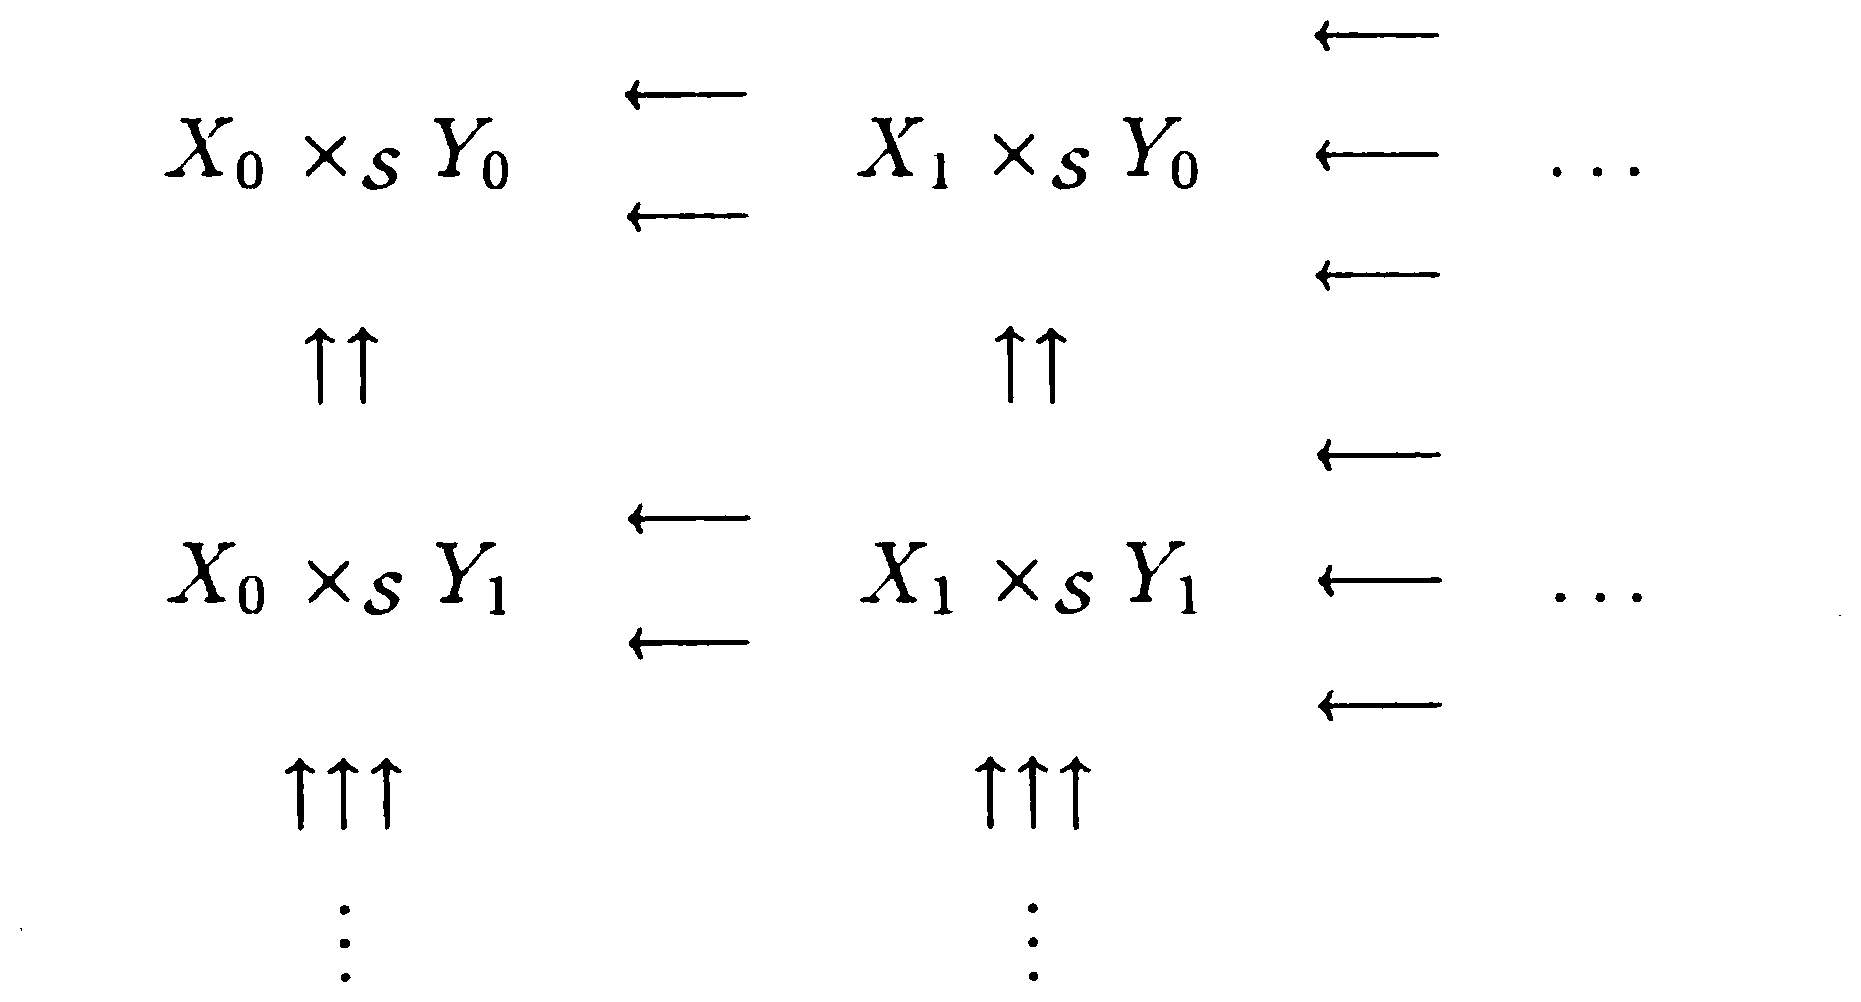
\includegraphics[width=0.62\linewidth]{fig_p22_a.png}
\end{center}
此时，由前面的注，
\[
X_i\times_SY_j=(X_i\times_SY_0)\times_{X_i}\cdots\times_{X_i}(X_i\times_SY_0)\qquad((j+1)\text{ 个})
\]
注意到这一点，便有$\mathbf{R}\Gamma(X_i,\mathbf{Q})\cong s(\mathbf{R}\Gamma(X_i\times Y_\bullet,\mathbf{Q}))$。

% ===== 原书 p.17 =====
因此$s(\mathbf{R}\Gamma(X_\bullet,\mathbf{Q}))\cong s(\mathbf{R}\Gamma(X_\bullet\times Y_\bullet,\mathbf{Q}))$。这里右边是双单纯概形的伴随单复形。另一方面，右边关于$X$与$Y$对称，故得到$s(\mathbf{R}\Gamma(X_\bullet\times Y_\bullet,\mathbf{Q}))\cong s(\mathbf{R}\Gamma(Y_\bullet,\mathbf{Q}))$。
\end{proof}

奇异同调也如下定义。令$C_\bullet(X,\mathbf{Q})$为$X$的$\mathbf{Q}$系数奇异同调。由此得到双复形
\[
\to C_\bullet(X_2,\mathbf{Q})\to C_\bullet(X_1,\mathbf{Q})\to C_\bullet(X_0,\mathbf{Q})
\]
把它的伴随单复形记作$C_\bullet(S,\mathbf{Q})$。其第$i$同调记作$H_i(S,\mathbf{Q})$。取 de Rham 实现（realization），便由积分得到自然的配对$H_i(S,\mathbf{Q})\otimes H^i(S,\mathbf{Q})\to\C$。

\transnote{原文把 $C_\bullet(X,\mathbf{Q})$ 称为「$X$ 的 $\mathbf{Q}$ 系数奇异同调」；严格说 $C_\bullet$ 是奇异链复形，其同调才是 $H_i$。译文照原文保留，此处仅作说明。}

其次定义迹映射。$S$为$\Spec(\C)$上紧合不可约代数叠时，存在与$S$同维的紧合不可约概形$X$与满射$\pi:X\to S$。把$\pi$的次数$\deg(X/S)$定义为：对支配态射$\varphi:Y\to S$，$\pi$的基变换$Y\times_SX\to Y$的次数；它是良定义的。把$X$的迹映射$\tr_X:H^{2d}(X,\mathbf{Q})\to\mathbf{Q}$（$d=\dim X$）与自然映射$\pi^*:H^{2d}(S,\mathbf{Q})\to H^{2d}(X,\mathbf{Q})$组合，令$\tr_S=(\deg(X/S))^{-1}\tr_X\circ\pi^*$，便定义迹映射$\tr_S$。它不依赖于$\pi:X\to S$的取法，这一点再由纤维积的讨论可知。

\subsection{$n$ 点稳定曲线的模理论}

Knudsen--Mumford 作为 Deligne--Mumford 结果的精密化，证明了$n$点稳定曲线的模问题可由代数叠表示。设$C,S$为基础域$k$上的有限型概形，$f:C\to S$与$n$个截面$s_1,\ldots,s_n:S\to C$是亏格$g$的稳定曲线，是指满足以下条件(1)--(5)。

\begin{enumerate}[label=(\arabic*)]
\item $f$在$S$上紧合平坦，相对维数为$1$。
\item 对各$s\in S$，纤维$f^{-1}(s)$既约，且至多只有通常二重点。
% ===== 原书 p.18 =====
\item $\dim H^1(f^{-1}(s),\mathcal{O}_{f^{-1}(s)})=g$。
\item $s_i(s)$包含在$f^{-1}(s)$的光滑点中。
\item $f^{-1}(s)$的有理分支包含$3$个以上的点，这些点是截面像$s_i(s)$或与其它分支的交点。
\end{enumerate}

令$\MbarGN$为亏格$g$的$n$点稳定曲线$(f:C\to S,s_1,\ldots,s_n)$的范畴，令$\MbarGN\to\Spec(k)$为把上述数据对应到$S$的函子，则它是代数叠。与前面一样，对概形$X$，给出$X\to\MbarGN$与给出亏格$g$的$n$点稳定曲线$(f:C\to X,s_1,\ldots,s_n)$等价。现在给定$(n+1)$点稳定曲线$(f:C\to S,s_1,\ldots,s_{n+1})$时，忘掉$s_{n+1}$，考虑$n$个截面$s_1,\ldots,s_n$。此时$(f:C\to S,s_1,\ldots,s_n)$一般不是$n$点稳定曲线；但考虑集合
\[
\begin{aligned}
\{s\in S\mid{}&\text{在 }f^{-1}(s)\text{ 中 }s_{n+1}\text{ 落在某个有理分支 }C_i\text{ 内，}\\
&\text{且 }C_i\text{ 只含 }s_i(s)\text{ 与其它分支的交点这 }3\text{ 个点}\},
\end{aligned}
\]
它定出$S$的闭子簇$Z$。设$C_i$为$f^{-1}(Z)$内与$C_i$对应的$\mathbf{P}^1$-丛（实际上，由于被$3$个点标记，它与$f^{-1}(Z)\times\mathbf{P}^1$同型）。此时$C_i\subset C$可以吹落，把结果所得的曲线记作$\bar f:\bar C\to S$。这时$(\bar f:\bar C\to S,s_1,\ldots,s_n)$是$n$点稳定曲线。$S$特别是一维且$C$光滑时，下面两个是典型的例子。

\begin{center}
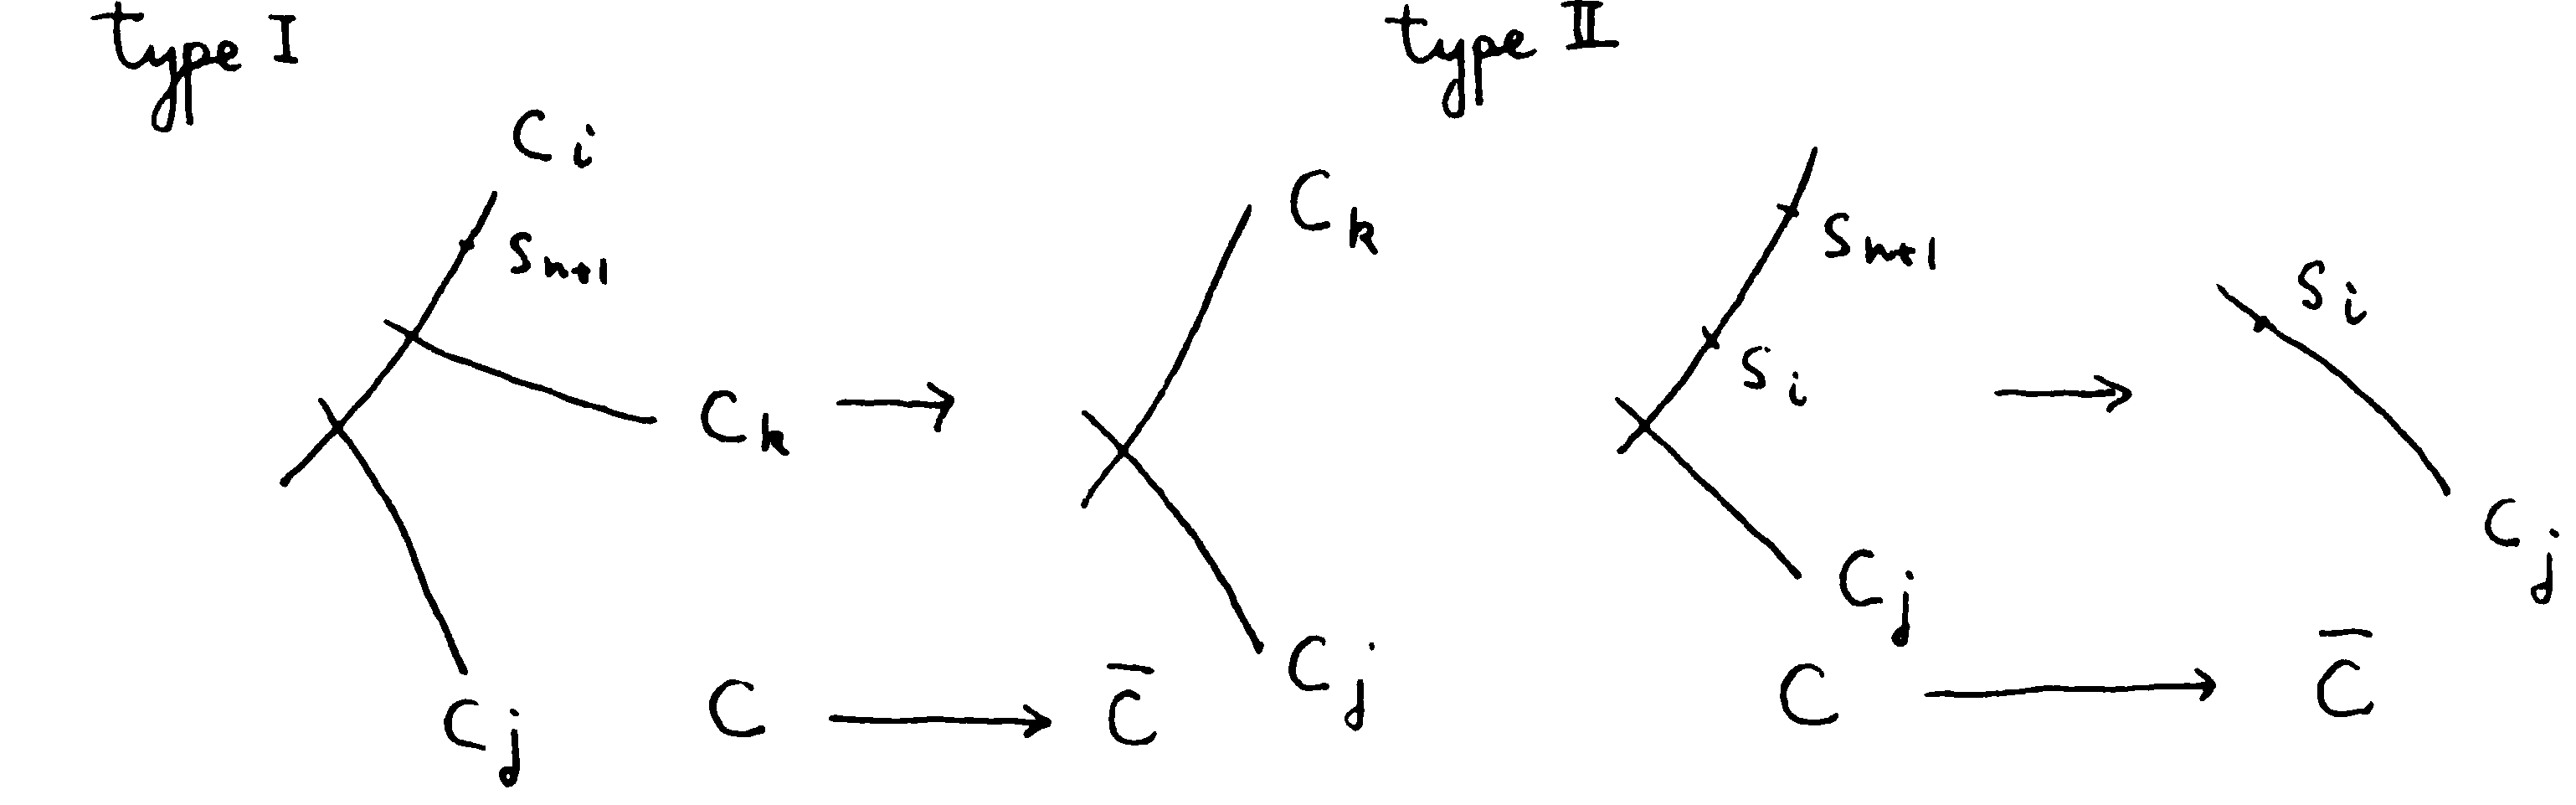
\includegraphics[width=0.9\linewidth]{fig_p24_a.png}
\end{center}

由此得到函子$\MbarN{g,n+1}\to\MbarGN$。

\begin{theorem}[Knudsen--Mumford {[KM]}]
\begin{enumerate}[label=(\arabic*)]
\item 现给定$X\to\MbarGN$，即给定亏格$g$的$n$点稳定曲线$(f:C\to X,s_1,\ldots,s_n)$。此时
% ===== 原书 p.19 =====
$C$自然同构于$\MbarN{g,n+1}\times_{\MbarGN}X$，$f$经此同构与第二投影$\MbarN{g,n+1}\times_{\MbarGN}X\to X$等同（视为同一）。
\item $\MbarGN$是紧合光滑代数叠。
\end{enumerate}
\end{theorem}

由(1)的性质，称$\MbarN{g,n+1}\to\MbarGN$为万有曲线。特别地，$\MbarN{g,1}\to\MbarG$是$\MbarG$上的万有曲线。其次构造万有截面$\tilde s_i:\MbarGN\to\MbarN{g,n+1}$（$i=1,\ldots,n$）。对$\MbarGN$的对象$(f:C\to X,s_1,\ldots,s_n)$，$s_i(X)$是$C$的除子。沿它在$X\times\mathbf{P}^1$内把除子$X\times\{0\}$粘到$C$上，把所得对象记作$\tilde C$。再定义两个截面$s'_i,s_{n+1}:X\to\tilde C$，分别由$X\to X\times\{1\}$、$X\to X\times\{\infty\}$给出。此时$(\tilde f:\tilde C\to X,s_1,\ldots,s'_i,\ldots,s_n,s_{n+1})$是$(n+1)$点稳定曲线。由此得到万有截面$\tilde s_i:\MbarGN\to\MbarN{g,n+1}$。

\begin{center}
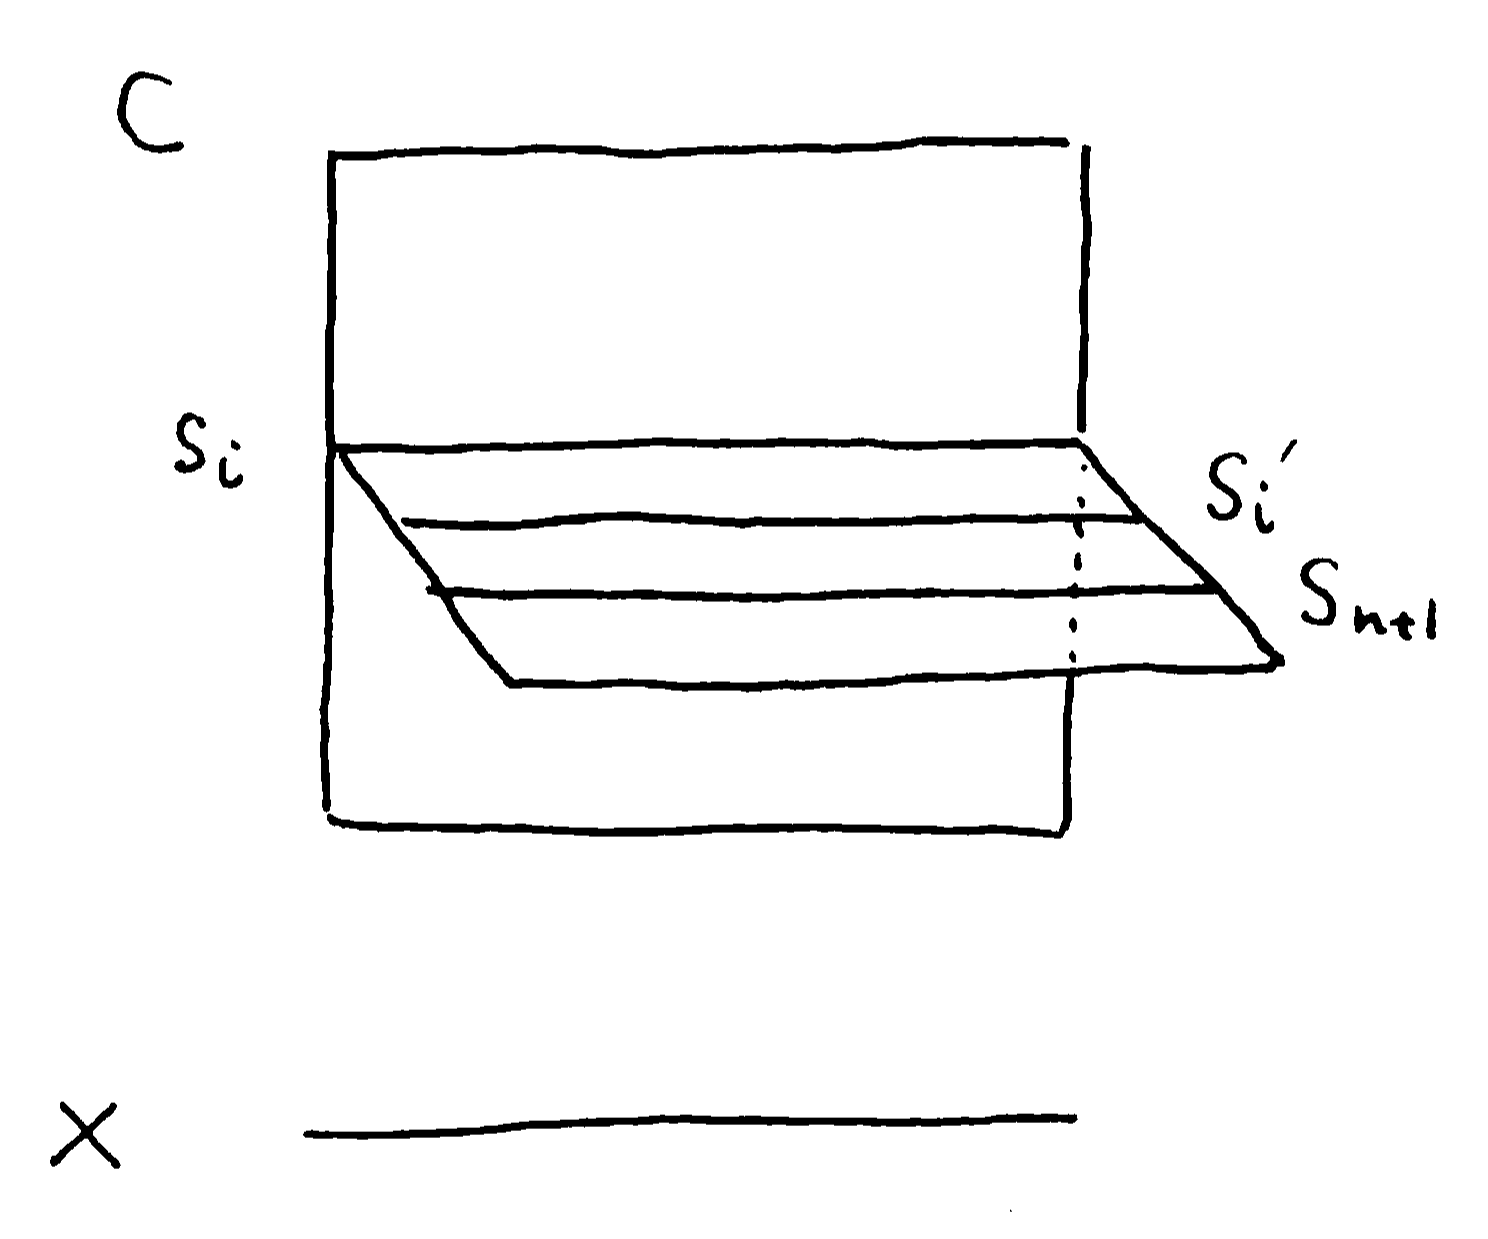
\includegraphics[width=0.55\linewidth]{fig_p25_a.png}
\end{center}

% =====================================================================
%  c03 —— PDF p.26–33（原书 p.20–27）
%  §2 二次微分的理论；§2.1 二次微分决定的叶状结构；§2.2 二次微分形式与带状图
% =====================================================================

% ===== 原书 p.20 =====
% §2（原书印「§2. QUADRATIC DIFFERENTIAL の理論」）
\section{二次微分的理论}
% §2.1（原书印「§2.1 QUADRATIC DIFFERENTIAL の定める FOLIATION」）
\subsection{二次微分决定的叶状结构}

本章说明 Strebel 的紧 Riemann 面（或者在它上面给定相异$n$点）上的二次微分理论。
参考书为[St]。这一理论不得不使用单变量函数论中的解析手法，正因如此才可以应用于模空间的胞腔分解。
二次微分的存在性，其理论根据在于从正规族中取出收敛的函数列。

设$X$为紧 Riemann 面，$p_1,\dots,p_n$为$X$上相异点，$D$为由$p_1+\dots+p_n$定义的除子。
$(X,p_1,\dots,p_n)$的二次微分$\omega$，指$(\Omega^1(D))^{\otimes2}$的整体截面。
以下在各点$p_i$处取其单值化参数（uniformizing parameter）$z_i$时，$\omega$可写成
\[
\omega=(a_{-2}z_i^{-2}+a_{-1}z_i^{-1}+\cdots)dz_i^{\otimes2},
\]
此时假定$a_{-2}\neq0$。这时在$X-\{p_1,\dots,p_n\}-(\omega)_0$（此处$(\omega)_0$为$\omega$的零点）上
有两种叶状结构（foliation）$F_r$、$F_i$，定义如下。

取$x\in X-\{p_1,\dots,p_n\}-(\omega)_0$的充分小邻域$U$及其上的单值化参数$z$，则$\omega$可写成
\[
\omega=f(z)dz^{\otimes2},\qquad f(z)=(a_0+a_1z+\cdots)dz^{\otimes2},
\]
其中$a_0\neq0$。于是除$\pm$号外存在唯一的$g(z)$，使$g(z)^2=f(z)$。
令$\psi(z)=\int_x^zg(z)$，则$\omega=\psi(z)$仍是$x$处的单值化参数。（必要时换用充分小的$U$。）
$U$上的曲线族$F_r|_U$，定义为由$T_{r,a}=\{z\mid\psi(z)\in a+i\R\}$（$a\in\R$）给出的族。
因$\psi(z)$除$\pm$号外唯一确定，$F_r|_U$在$X-\{p_1,\dots,p_n\}-(\omega)_0$上决定叶状结构。
同样，$F_i|_U$定义为由$T_{i,b}=\{z\mid\psi(z)\in\R+bi\}$（$b\in\R$）确定的曲线族，
再同样定义整体的$F_i$。又$\psi(z)\colon U\xrightarrow{\ \sim\ }D\subset\C$诱导$\C$的平坦度量，
故$U$上有平坦度量。而$\psi(z)$由$\omega$除$\pm1$外唯一确定，且积分起点的更换只引起平移，
因此在$X-\{p_1,\dots,p_n\}-(\omega)_0$上诱导平坦度量。称之为由$\omega$决定的平坦度量。
对$X$的子集$U$，用$\omega$决定的度量量出的面积记作$\|\omega\|_U$。

\transnote{原文此处把$f(z)$写成$(a_0+a_1z+\cdots)dz^{\otimes2}$，即$dz^{\otimes2}$重出了一次；
下一句又把$\psi(z)$误印作$\omega$。两句均照原文排印。}

下面看$F_r$在$p_1,\dots,p_n$以及$(\omega)_0$处的样子。

（1）$p_1,\dots,p_n$处的样子。设$p_i$处的局部参数为$z$，则$\omega=(a_{-2}z^{-2}+$
% ===== 原书 p.21 =====
$a_{-1}z^{-1}+\cdots)dz^{\otimes2}$，且$a_{-2}\neq0$，故存在某个$g(z)$，
使$g(z)=(b_{-1}z^{-1}+b_0+\cdots)$，其中$b_{-1}\neq0$。
取$p_i$的充分小邻域$U$以及$U-\{p_i\}\ni p_0$，令$\psi(z)=\int_{p_0}^zg(z)dz$。
$w=\psi(z)$是多值函数，记其反函数为$\tau$，则$\tau$是周期为
$\oint g(z)dz=2\pi i\cdot b_{-1}$的周期函数。
\[
\begin{array}{ccc}
\C\supset(\operatorname{Im}\psi) & \xrightarrow{\ \tau\ } & U-\{p_0\}\\[2pt]
\downarrow & & \downarrow\\[2pt]
w & \mapsto & \tau(w)
\end{array}
\]

现引入新变量$t=\exp\left(\frac{w}{b_{-1}}\right)$，则$t$是$U$上$p_i$周围的单值化参数。
属于$F_r$的曲线族由$w=b_{-1}\log(t)\in a+i\R$给出。此时
\[
t=\exp\left(\frac{a+i\theta}{b_{-1}}\right)=\exp\left(\frac{a}{b_{-1}}\right)\exp\left(\frac{i\theta}{b_{-1}}\right)
\qquad(\theta\in\R)
\]
是该曲线的参数表示，其图形按下列情形区分。

\begin{enumerate}[label=(\arabic*),leftmargin=2.6em,itemsep=2pt,topsep=4pt]
\item $b_{-1}\in\R$的情形。$T_a$是与绕$p_i$一周的$S^1$同胚的曲线，长度为$2\pi b_{-1}$。
\item $b_{-1}\in i\R$的情形。$T_a$同胚于连结$p_i$与另一点的半直线。
\item $b_{-1}\in\C-\R-i\R$。$T_a$呈涡旋状。
\end{enumerate}

\begin{center}
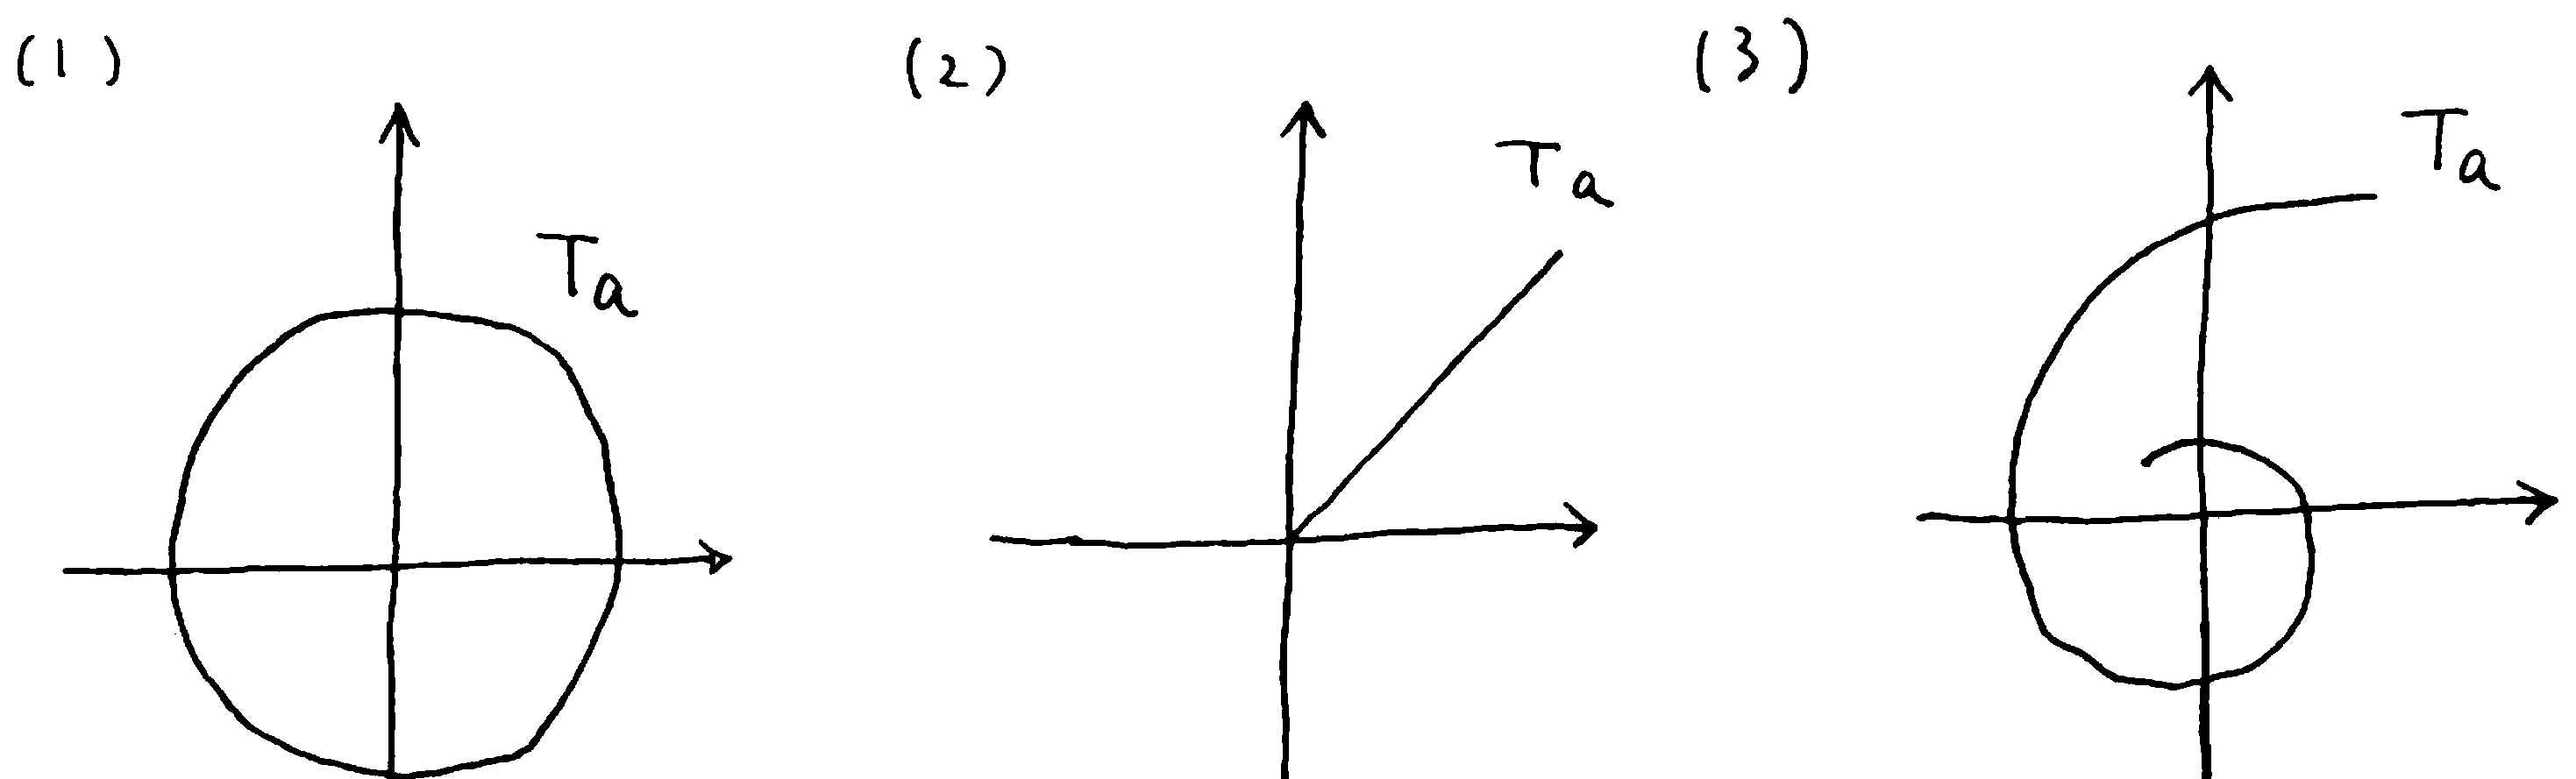
\includegraphics[width=0.75\linewidth]{fig_p27_a.png}
\end{center}

其次看$(\omega)_0$处的样子。设$\operatorname{ord}(\omega)=m>0$，则
$\omega=(a_mz^m+a_{m+1}z^{m+1}+\cdots)dz^{\otimes2}$，$a_m\neq0$。
故取满足$g(z)^2=a_mz^m+a_{m+1}z^{m+1}+\cdots$的$g(z)$，便有
$g(z)=b_{m/2}z^{m/2}+b_{m/2+1}z^{m/2+1}+\cdots$。

（1）$m$为偶数的情形。令$m=2m'$，则
$\psi(z)=\int g(z)dz=\frac{1}{m'+1}b_{m'}z^{m'+1}+\cdots$，
故$T_0$同胚于在原点相交的$m+2$条半直线。

% ===== 原书 p.22 =====
$T_a$如下图所示。

\begin{center}
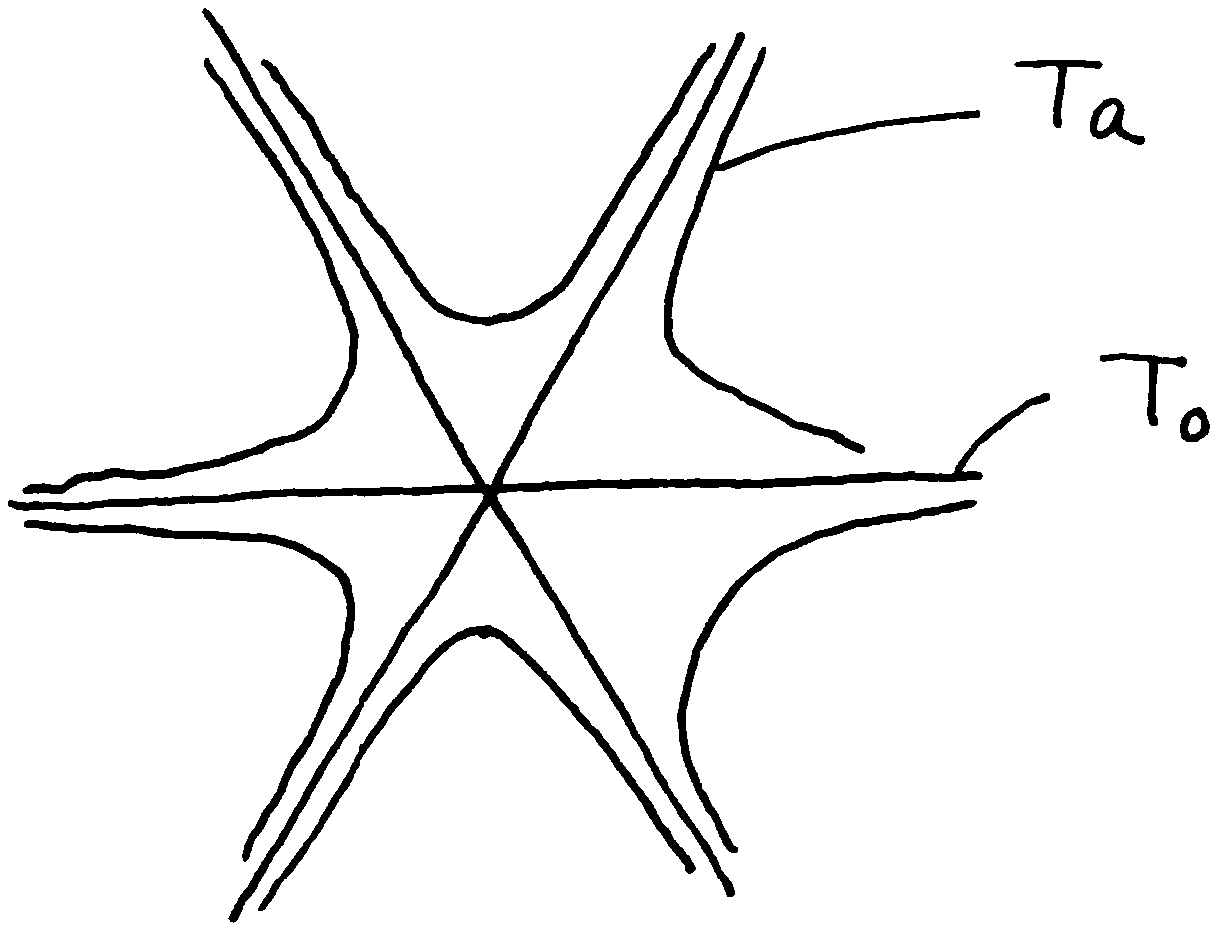
\includegraphics[width=0.42\linewidth]{fig_p28_a.png}
\end{center}

（2）$m$为奇数的情形。令$z^{1/2}=u$，在由$u$决定的分歧覆盖上，$\psi(z)$为
\[
\psi(z)=\frac{2}{m+2}b_{m/2}u^{m+2}+\cdots
\]
把它放回$z$平面上考虑，$T_0$仍同胚于在原点相交的$m+2$条半直线。
$T_a\cup T_{-a}$如下图所示。（此处须注意，$T_a\cup T_{-a}$不依赖于$u$的分支取法。）

\begin{center}
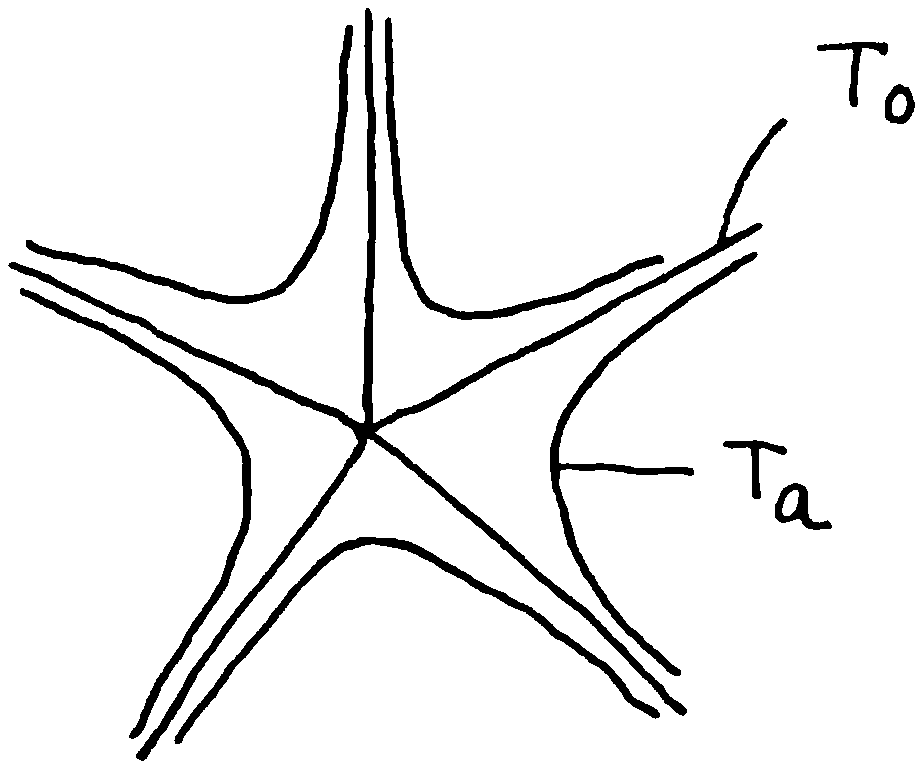
\includegraphics[width=0.38\linewidth]{fig_p28_b.png}
\end{center}

下面据此看$X$整体给出怎样的叶状结构。例如$X$的亏格为$1$，$p$为$X$上一点。
考察仅在$p$处有极点、在$q_0$与$q_1$处有单零点的二次微分$\omega$，
并且$p$处的展开系数为$b_{-1}\in\R$即$a_{-2}\in\R_{>0}$的情形。
此时出现下图那样的叶状结构。（这是切开的图。）

\begin{center}
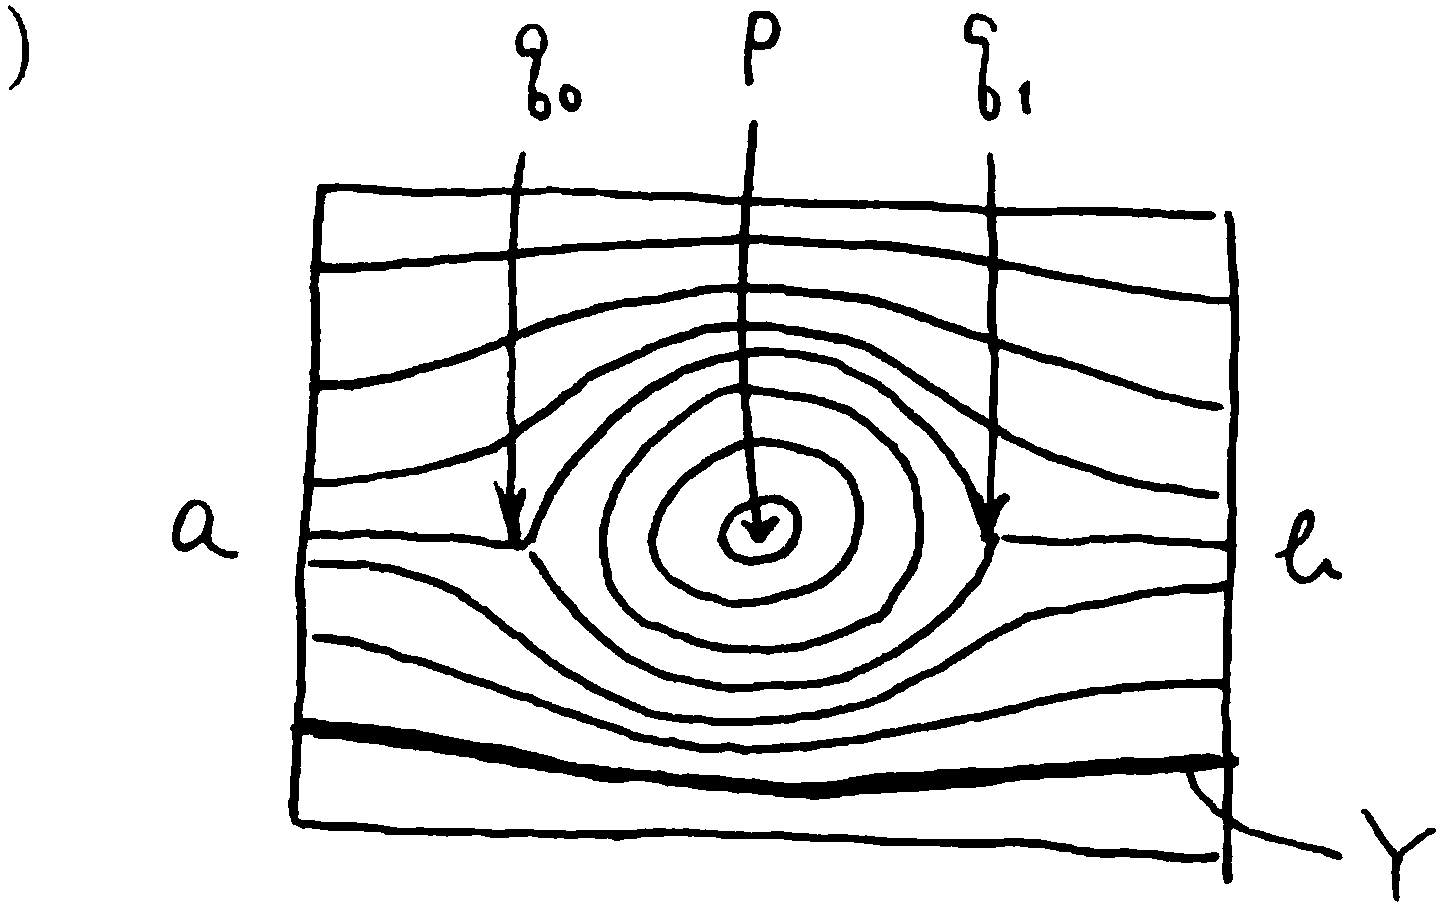
\includegraphics[width=0.55\linewidth]{fig_p28_c.png}
\end{center}

% ===== 原书 p.23 =====
此时，「$\omega$有单零点」这一条件在$H^0(X,(\Omega^1_X(D))^{\otimes2})$中是开条件，
而$a_{-1}\in\R_{>0}$是实余维$1$的条件。以$\R_{>0}$作乘法换掉$\omega$，叶状结构本身并不改变，
故上图以实$2$维自由度出现。须注意，图中$a$与$b$一致，$Y$附近的叶状结构同构于$S^1$，
这两件事等价。要使$a$与$b$一致，还须再加一个余维$1$的条件。
在该条件下把$\omega$取来换去，连结$q_0$与$q_1$的曲线绕$p$一周所得区域的面积随之改变。（下图）

\begin{center}
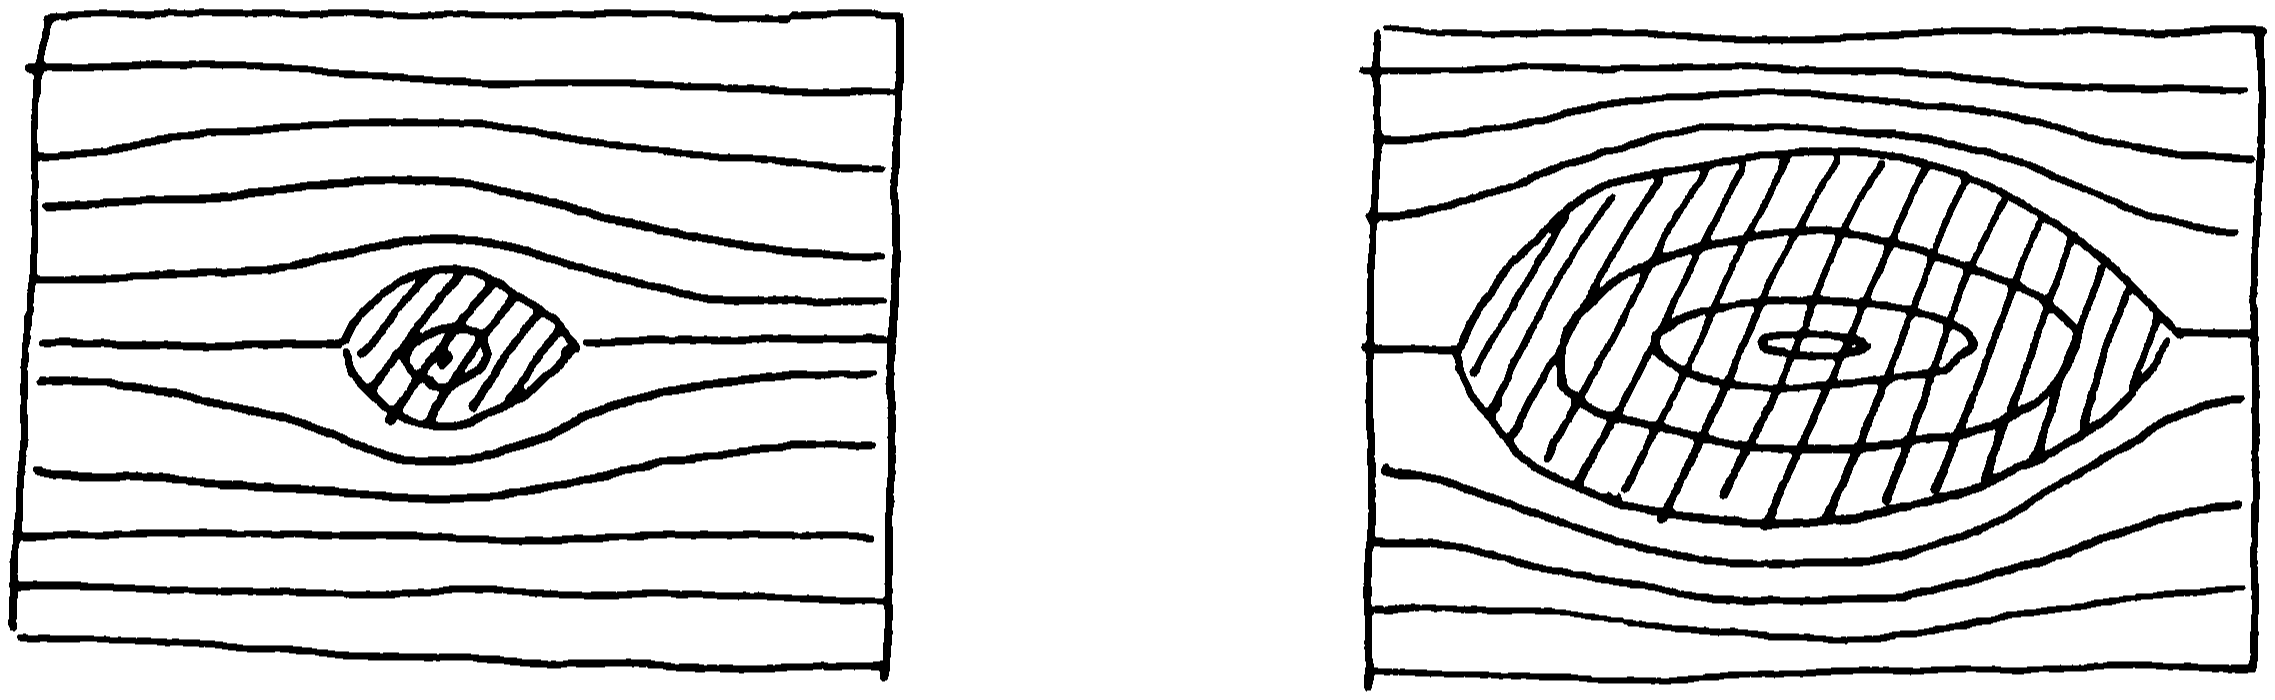
\includegraphics[width=0.6\linewidth]{fig_p29_a.png}
\end{center}

取有一维参数的参数族，使面积不断增大，则应落到
$H^1(X,(\Omega^1_X(D))^{\otimes2})-\{0\}/\R^+\cong S^3$中某点。
若一切顺利，可以预测只能取到唯一一个这样的二次微分：图中斜线部分占去几乎所有的点。
后文可知这是正确的。此时成下图。粘合的状况一般如上图那样。

\begin{center}
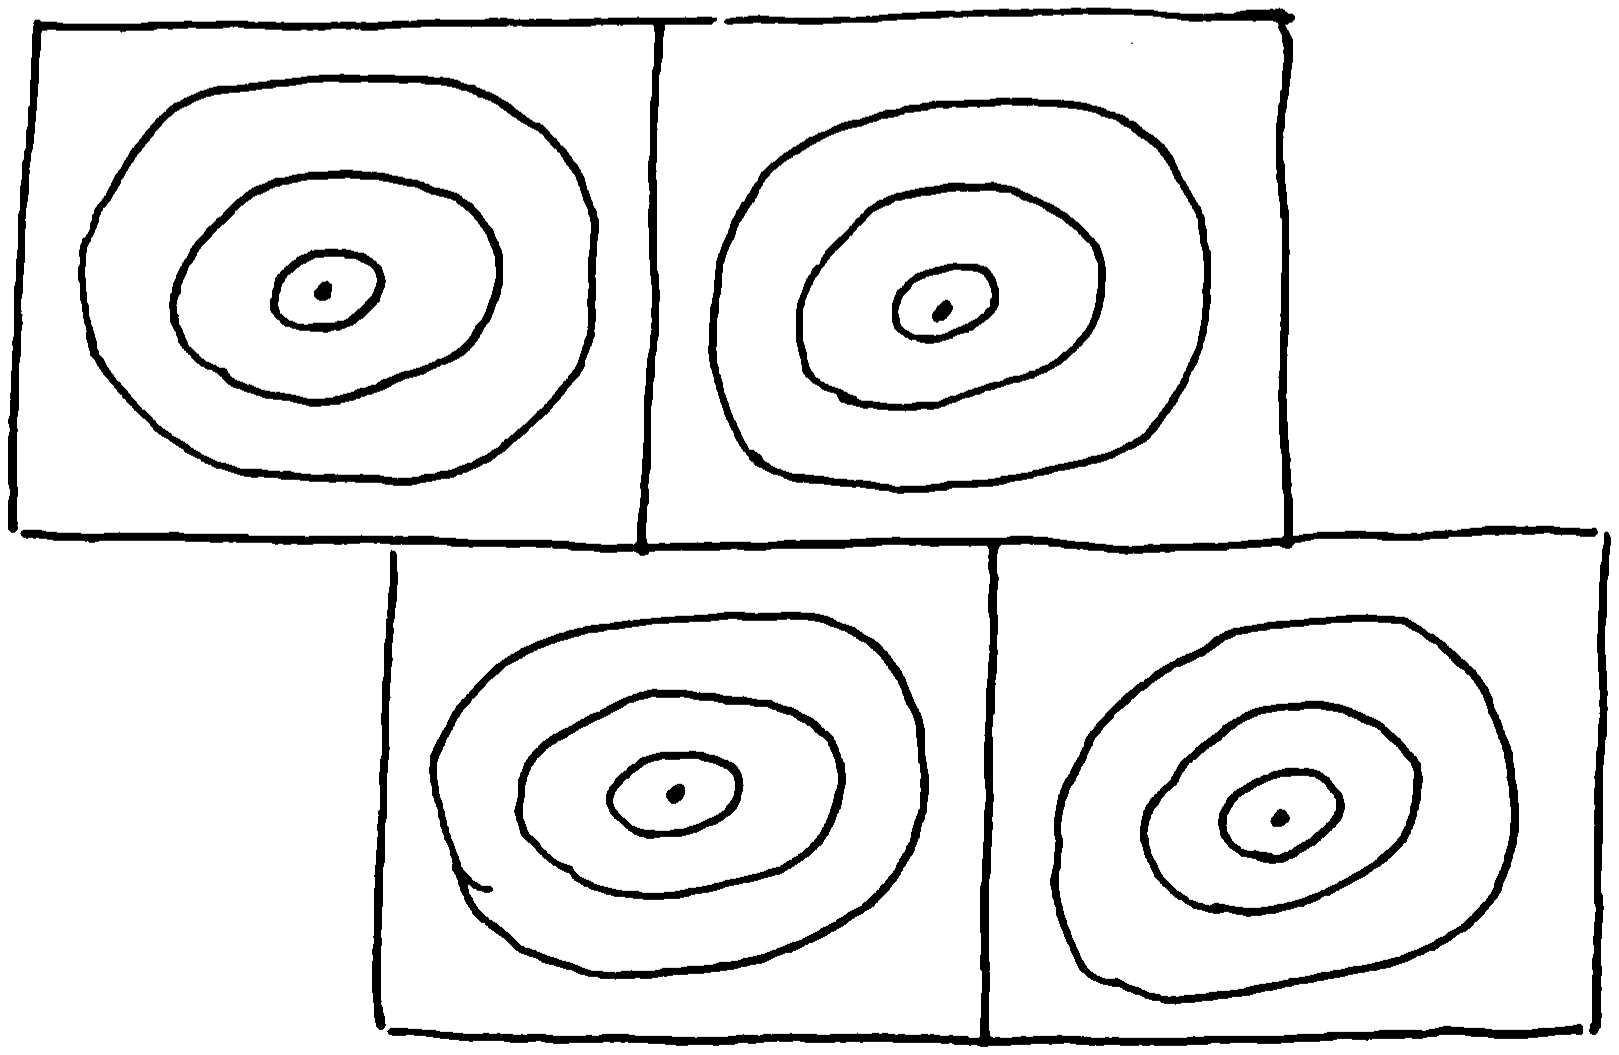
\includegraphics[width=0.6\linewidth]{fig_p29_b.png}
\end{center}

% ===== 原书 p.24 =====
进而，把与$p$周围小闭曲线同伦的、同胚于$S^1$的轨道全部除去，则得下图那样的$1$-骨架。

\begin{center}
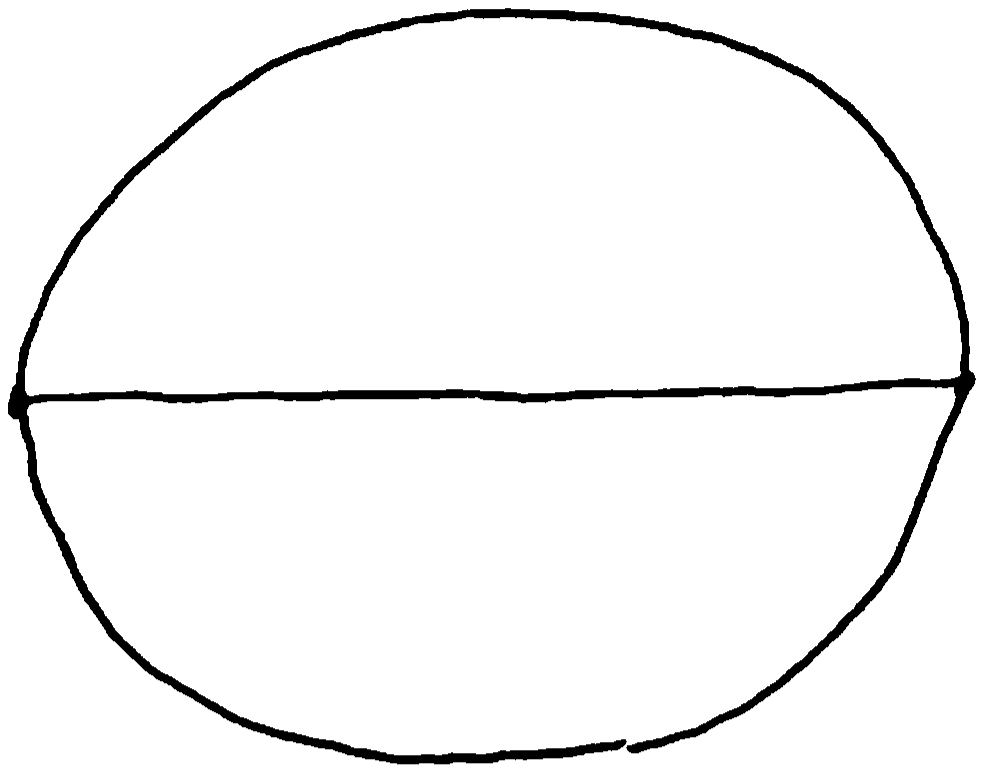
\includegraphics[width=0.3\linewidth]{fig_p30_a.png}
\end{center}

这样给出椭圆曲线与$1$点后，以$\R_{>0}$为模，上图那样的图型只有$1$种。
（实际上依椭圆曲线不同，也出现下图那样的情形。）

\begin{center}
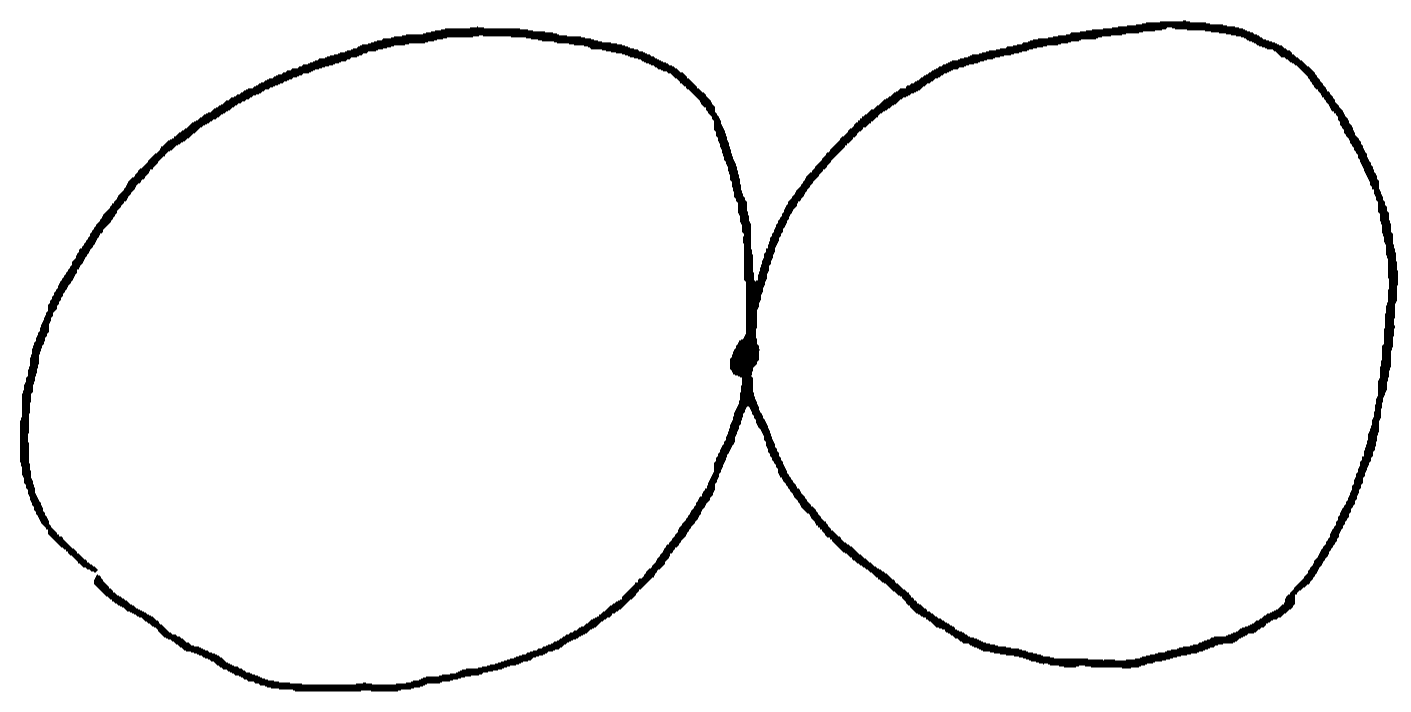
\includegraphics[width=0.34\linewidth]{fig_p30_b.png}
\end{center}

证明这种二次微分的存在与唯一性，是本章的目的。

% Theorem 2.1（原书印 Theorem 2.1）
\begin{theorem}
设$X$为紧 Riemann 面，$p_1,\dots,p_n$为$X$上相异的$n$点，$r_1,\dots,r_n$为$\R_{>0}$的元。
此时存在唯一的二次微分，具有下列性质。
\begin{enumerate}[label=(\arabic*),leftmargin=2.6em,itemsep=2pt,topsep=4pt]
\item 在$p_i$周围，$\omega$有下列展开
\[
\omega=\left(r_iz_i^{-2}+O\left(\frac{1}{z}\right)\right)dz^{\otimes2}
\]
\item 取$\gamma_i$为$p_i$周围的小闭曲线，则
\[
X^{(1)}=X-\bigcup_{i=1}^n\{\delta\mid\delta\text{是与}S^1\text{同胚的轨道，且与}\gamma_i\text{同伦}\}
\]
是$X$的测度$0$集。
\end{enumerate}
\end{theorem}

% ===== 原书 p.25 =====
此外，此时$X^{(1)}$为$1$维 CW 复形。

证明将在§2.3、§2.4给出。

% Definition 2.1（原书印 Definition 2.1）
\begin{definition}
具有定理 2.1 的(2)的性质的二次微分，称为具闭轨道的二次微分。
\end{definition}

% §2.2（原书印「§2.2 QUADRATIC DIFFERENTIAL FORM と RIBBON GRAPH」）
\subsection{二次微分形式与带状图}

现给定 Riemann 面$X$及其上$n$点$p_1,\dots,p_n$以及$r_1,\dots,r_n\in\R_+=\{r\in\R\mid r>0\}$时，
考虑满足定理 2.1 条件的二次微分$\omega$。
在$X^0-\{p_1,\dots,p_n\}-(\omega)_0$上，如前所述由$\omega$决定平坦度量，
由此在$X^{(1)}$上诱导度量。又$X^{(1)}$位于$X$上，故在下列意义下成为带状图（ribbon graph）。

% Definition 2.2（原书印 Definition 2.2 (ribbon graph)）
\begin{definition}[带状图]
无边界的一维 CW 复体$K$（即对任意顶点，以它为端点的棱至少有$2$条）具有带状结构（ribbon
structure）$R$，指的是对每个顶点$v$，在$E_v=\{e:\text{棱}\mid v\text{是}e\text{的端点}\}$上
定好循环次序。用图表示循环次序时，使用下图中任一个。
\end{definition}

\begin{center}
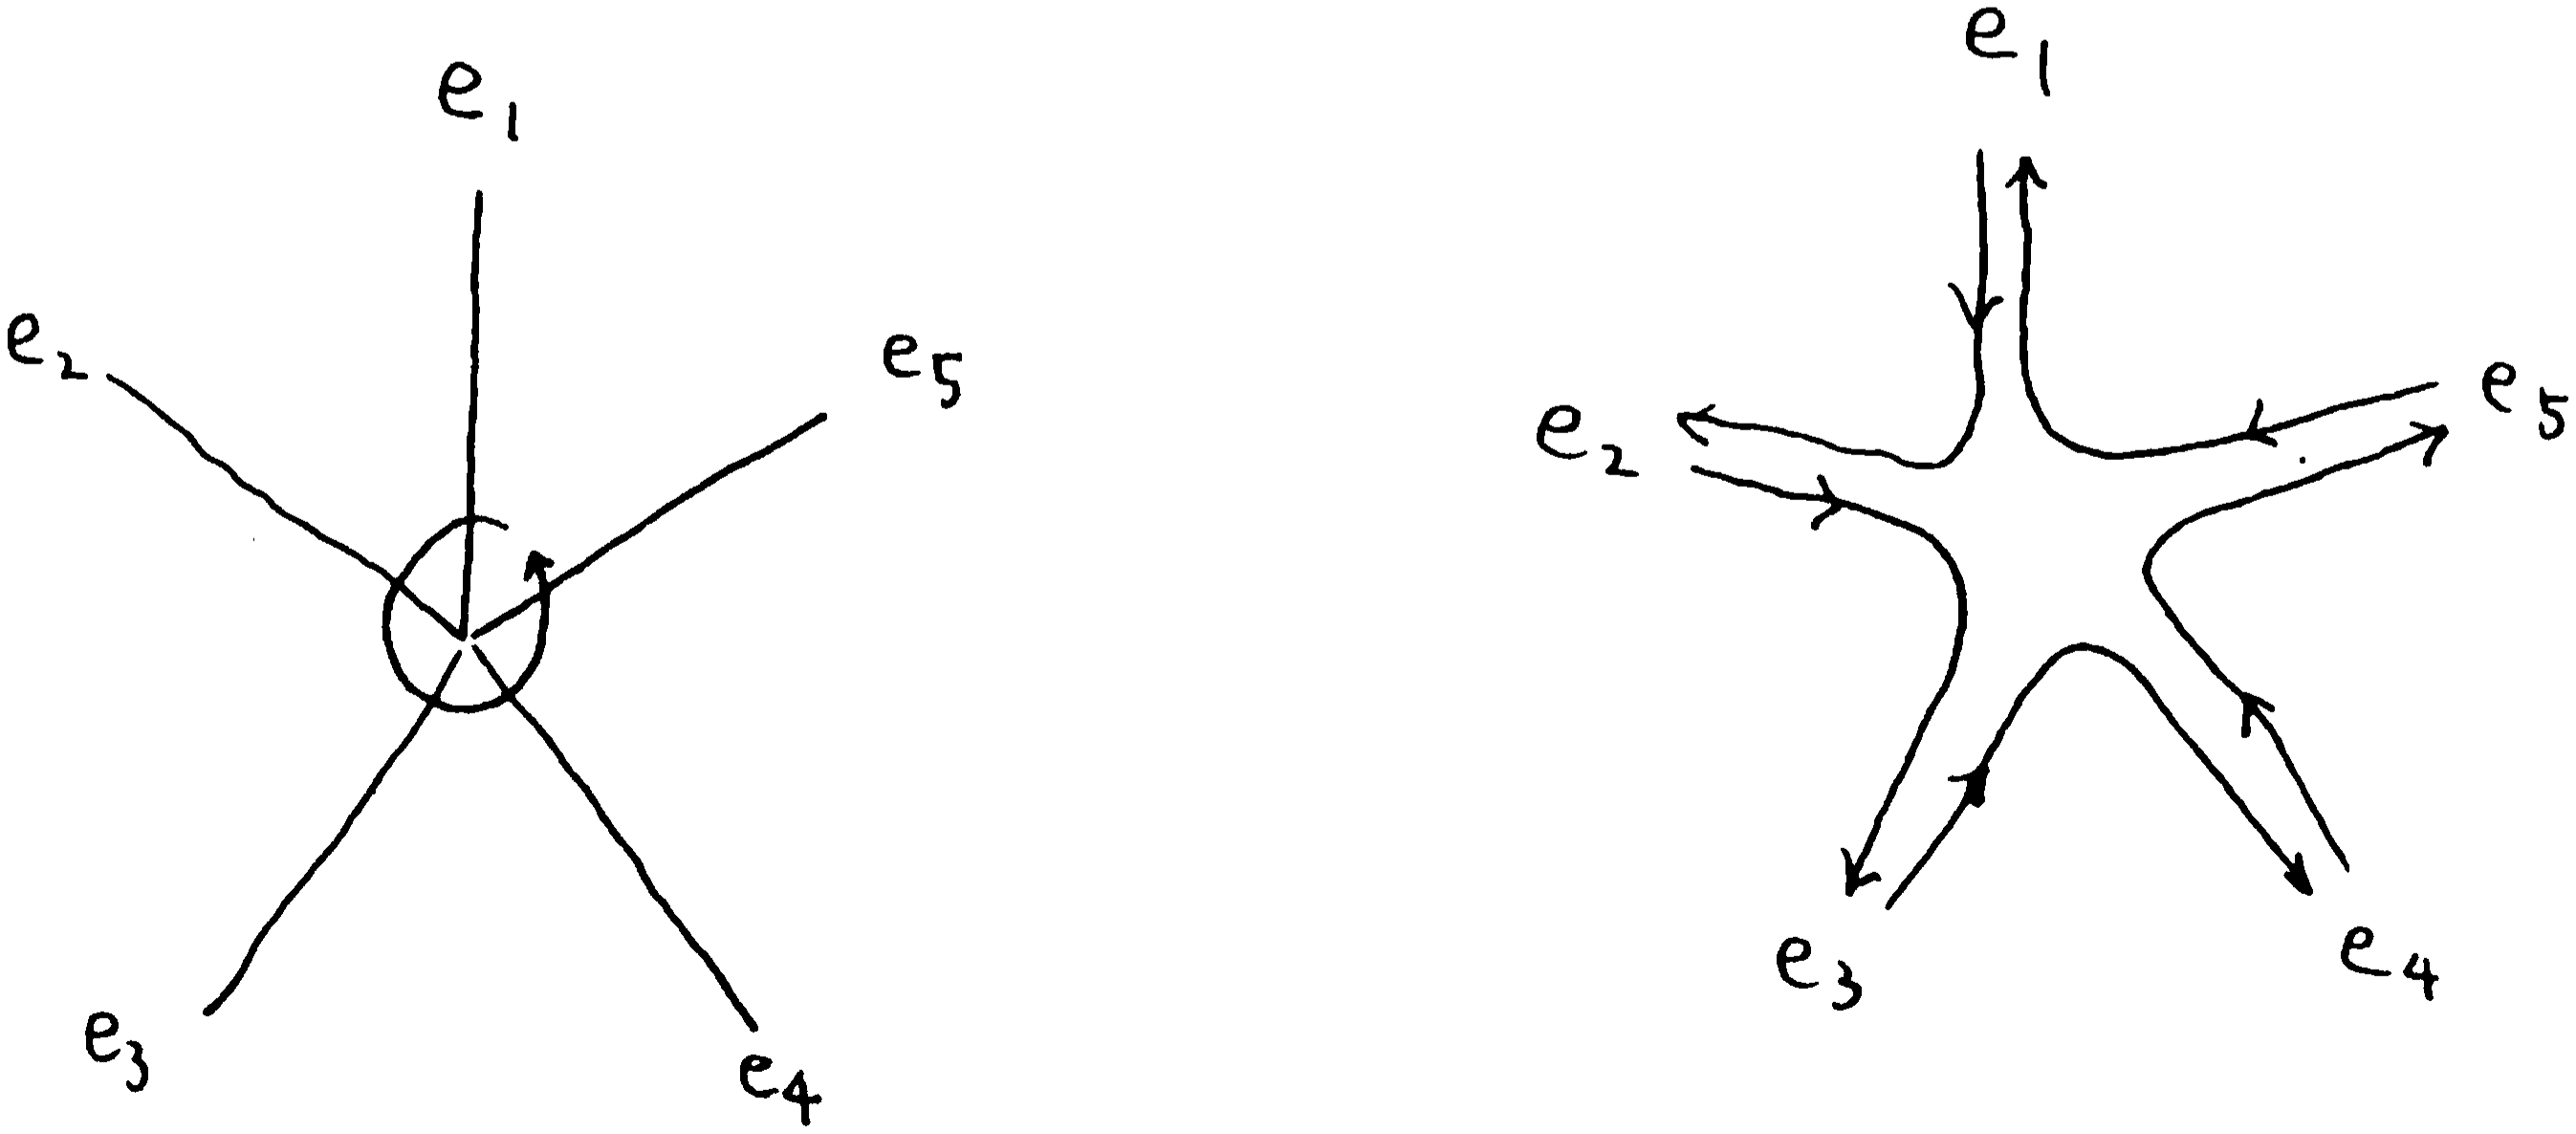
\includegraphics[width=0.72\linewidth]{fig_p31_a.png}
\end{center}

% Example（原书印 Example.，未编号；按原书排成不编号的黑体提示语，不占 example 计数器）
\noindent\textbf{例.}
设$K$为由顶点集$V(K)=\{v_1,v_2\}$、棱集$E(K)=\{e_1,e_2,e_3\}$给出，
且$e_i$（$i=1,2,3$）的端点集表为$\operatorname{end}(e_i)=\{v_1,v_2\}$的图。

% ===== 原书 p.26 =====
\begin{center}
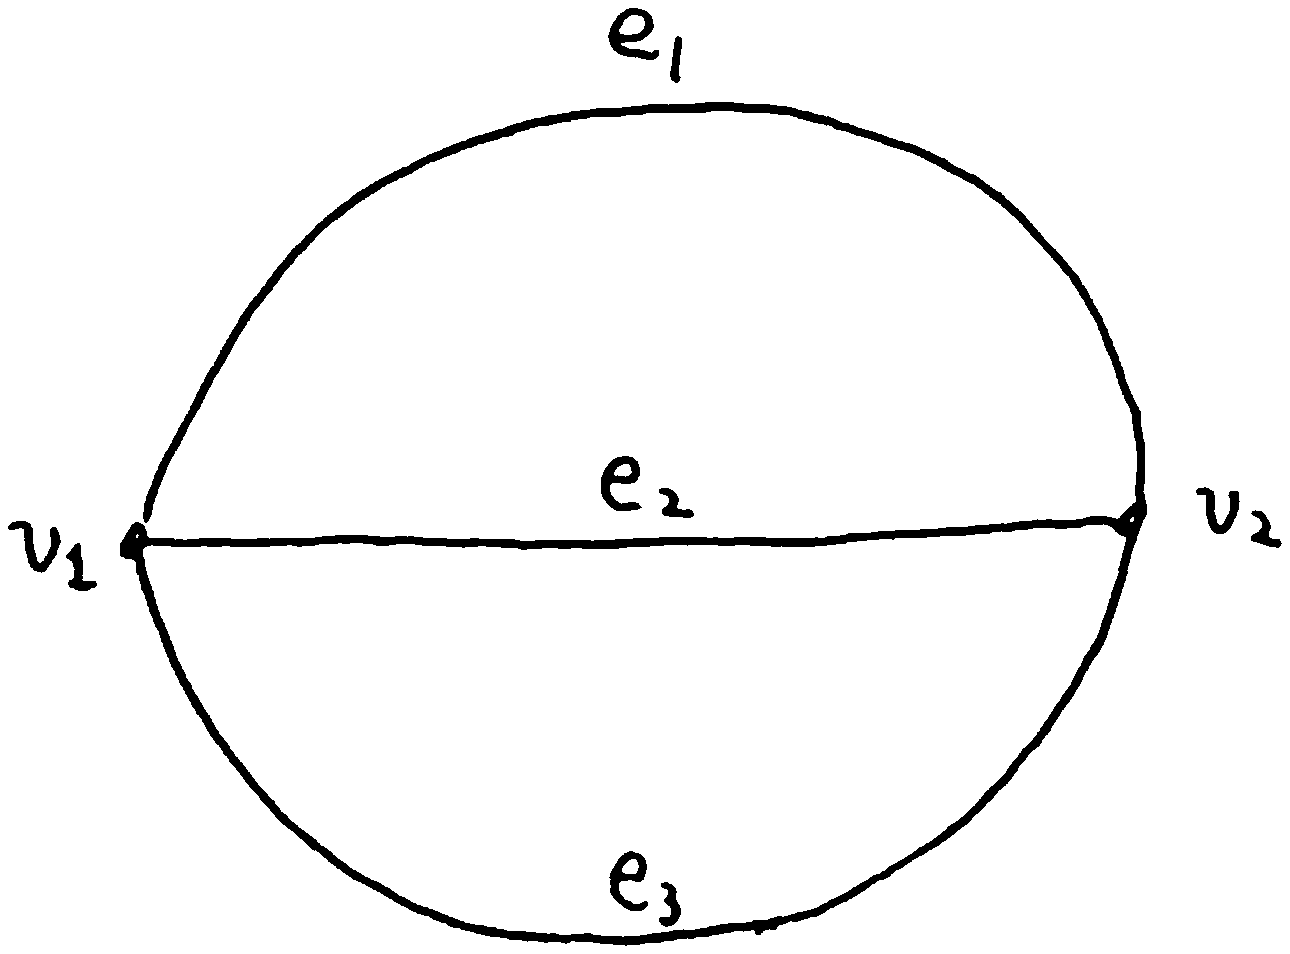
\includegraphics[width=0.32\linewidth]{fig_p32_a.png}
\end{center}

$E(v_1)=\{e:\text{棱}\mid v_1\text{是}e\text{的端点}\}$的循环次序给定为$e_3\to e_2\to e_1$，
$E(v_2)$的循环次序给定为$e_3\to e_2\to e_1$时，其带状图如下表示。

\begin{center}
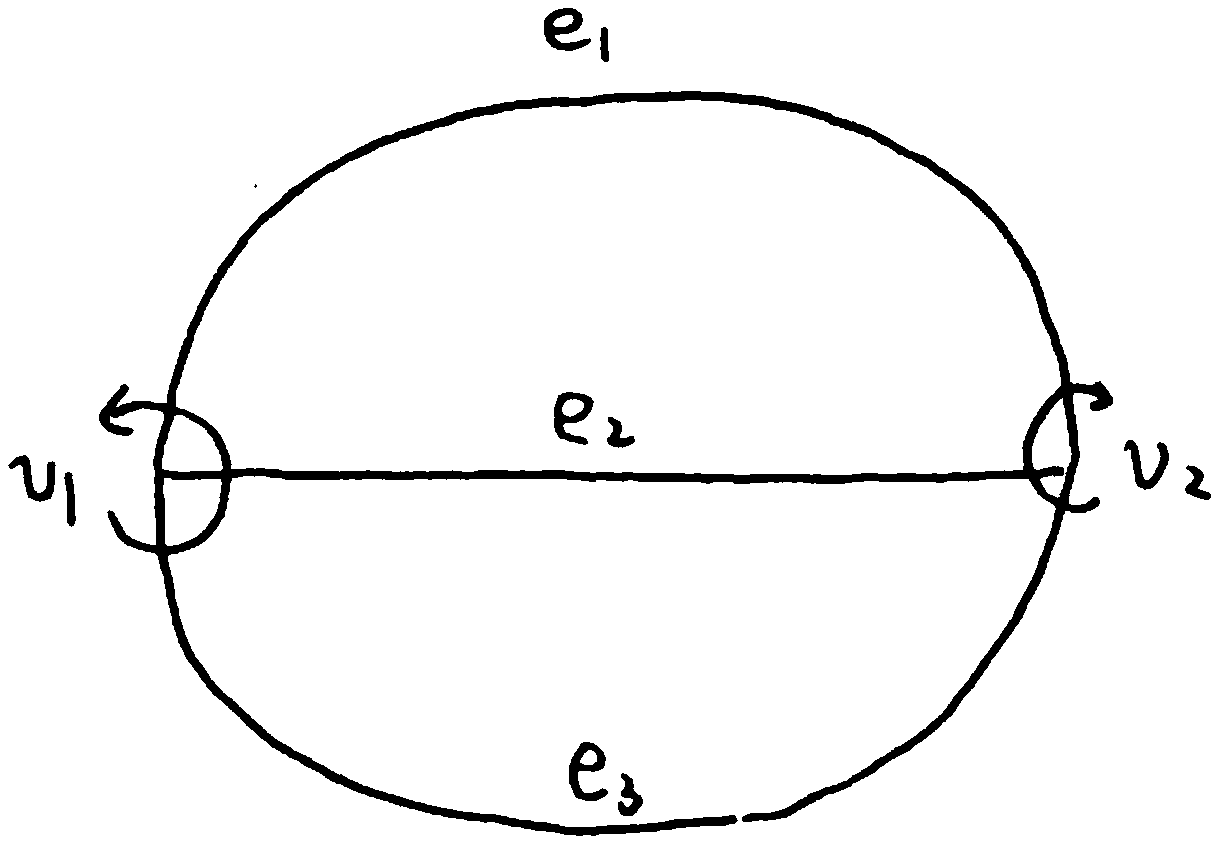
\includegraphics[width=0.40\linewidth]{fig_p32_b1.png}\hspace{1.5em}或\hspace{1.5em}%
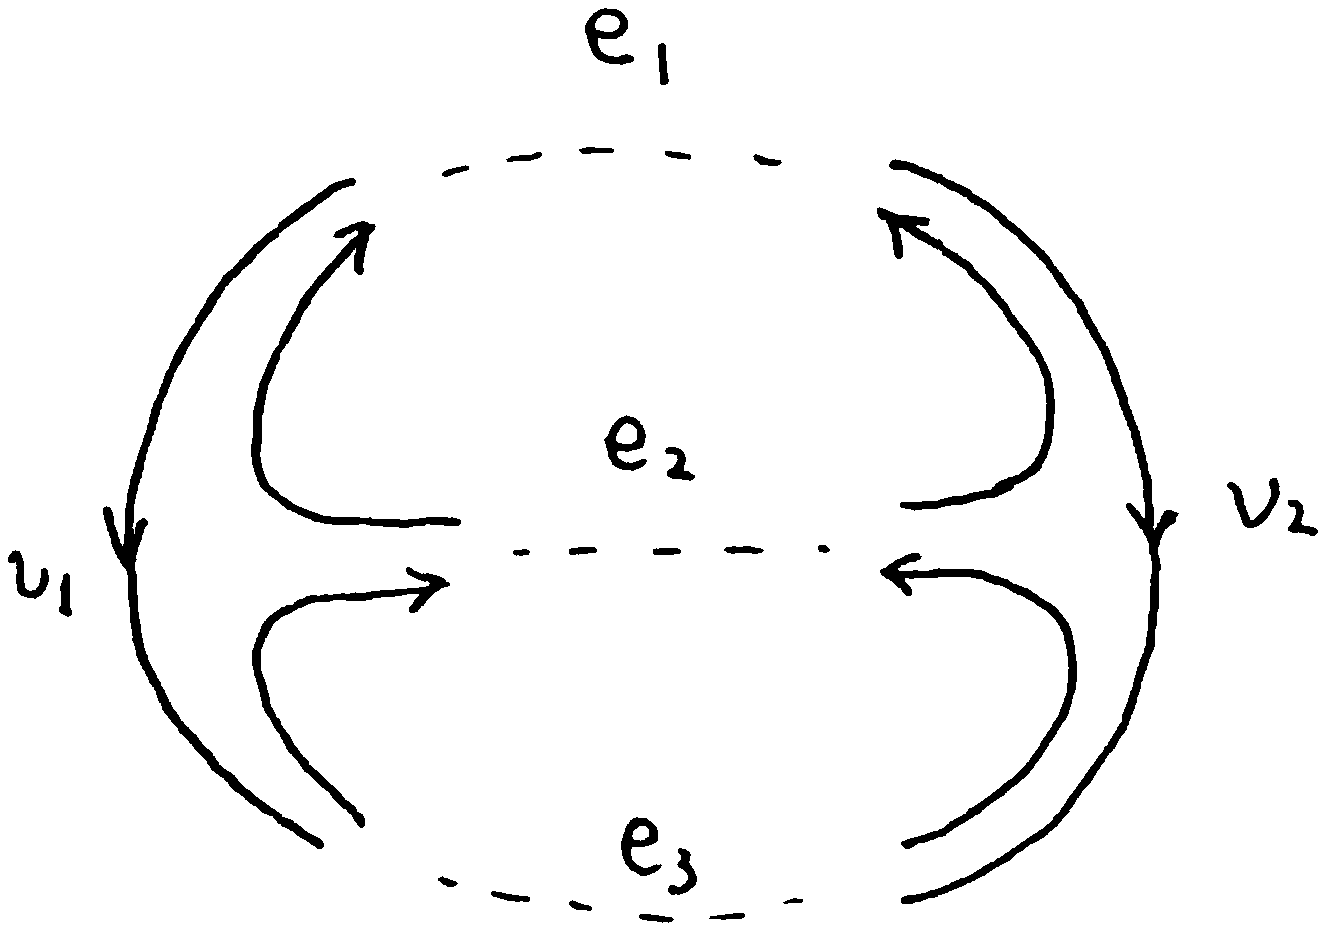
\includegraphics[width=0.40\linewidth]{fig_p32_b2.png}
\end{center}

后一情形也有把两侧带方向的带状长条插入棱中、使整体箭头相连来表示的做法。（下图）

\begin{center}
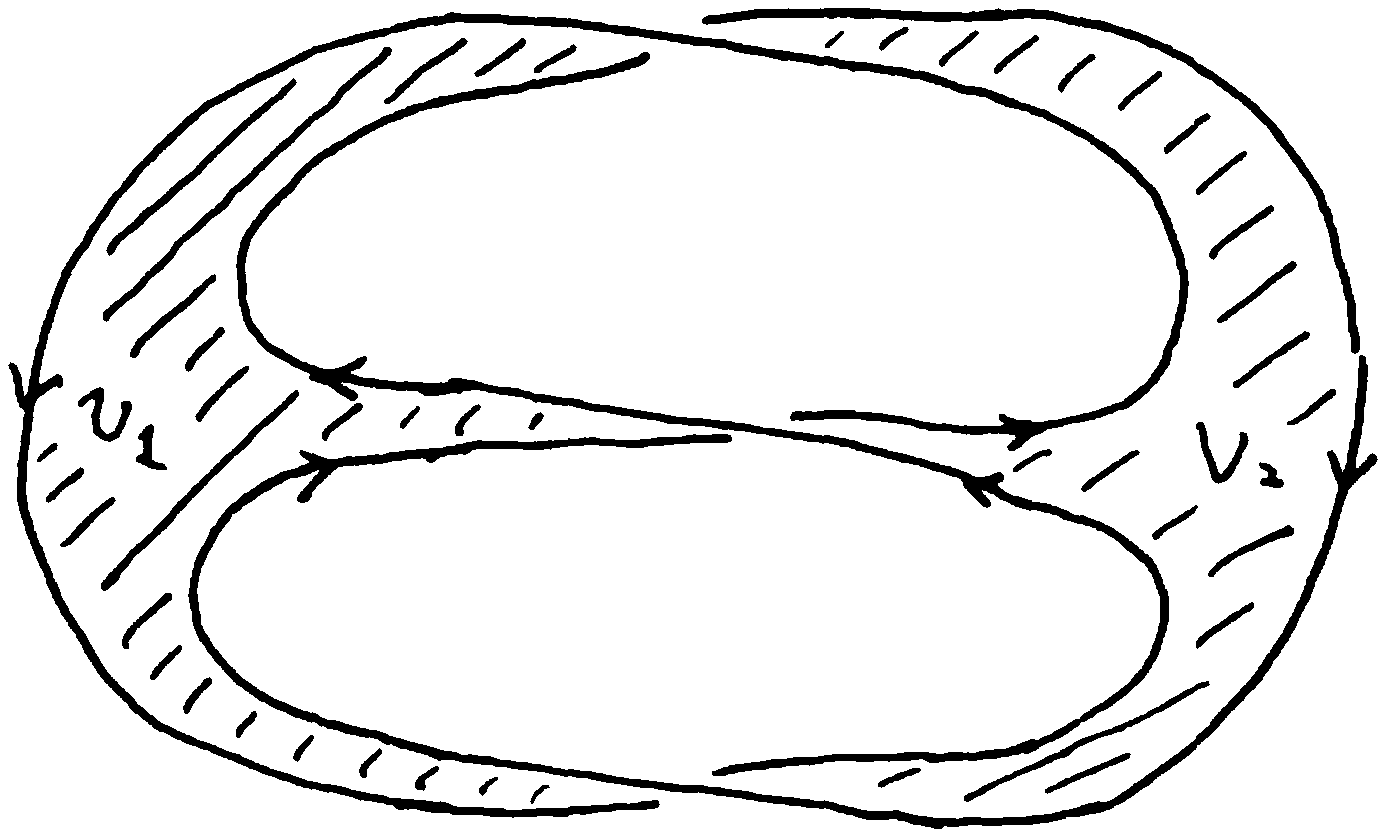
\includegraphics[width=0.45\linewidth]{fig_p32_c.png}
\end{center}

% Definition 2.3（原书印 Definition 2.3 (metrized ribbon graph)）
\begin{definition}[带度量带状图]
带状图$(K,R)$上的度量结构（metric structure），指给带状图的每条棱赋正数$l_i$作为「长度」。
\end{definition}

这样，由 Riemann 面、其上$n$点以及正数$r_1,\dots,r_n$的组
$(X,p_1,\dots,p_n,r_1,\dots,r_n)$这样的数据，构成带度量带状图$(K,R,M)$，而$X$的

% ===== 原书 p.27 =====
亏格$g=g(X)$及点的个数$n$，可从$(K,R,M)$如下读出。
首先，把带状图如图 1 那样表示时，边界的个数即给出$n$。
进而，$K$作为拓扑空间的 Euler 数$=\#V(K)-\#E(K)$等于$2-2g-n$，由此可读出$g$。即
\[
g=\frac{1}{2}(2-n+\#E(K)-\#V(K)).
\]
称$(g,n)$为带状图的型。即使图相同，带状结构的给法不同，其型$(g,n)$也会改变。
例如下图(1)为$(g,n)=(1,1)$，(2)为$(g,n)=(0,3)$。

\begin{center}
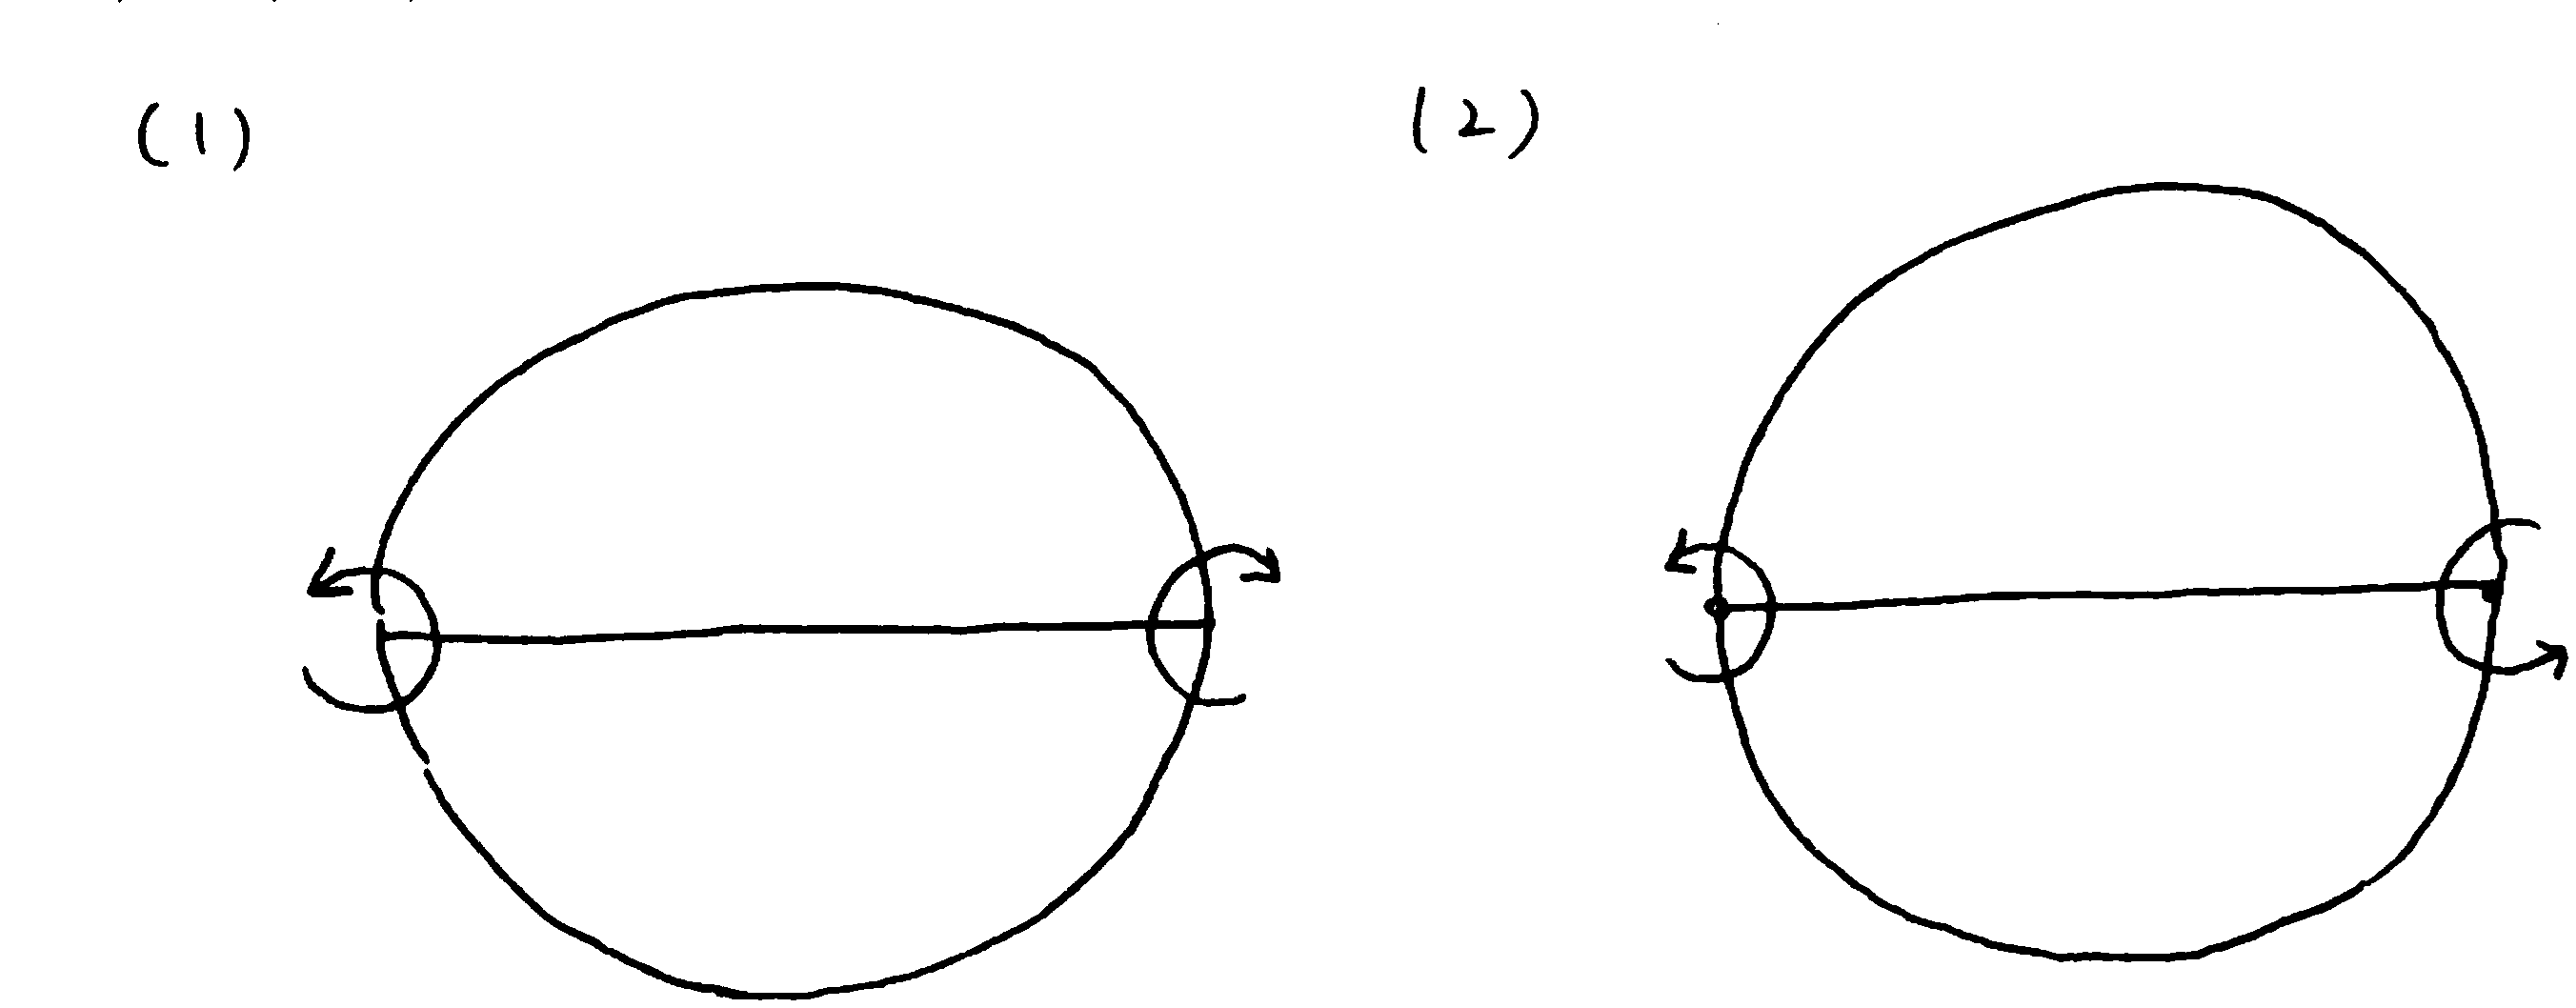
\includegraphics[width=0.6\linewidth]{fig_p33_a.png}
\end{center}

最后，给定带度量带状图$(K,R,M)$时，构造 Riemann 面$X$、其上点$p_1,\dots,p_n$以及在
$p_1,\dots,p_n$处有二阶极点的二次微分$\omega$，使由此得到的带度量带状图为$(K,R,M)$，
以此结束本节。设带状图的边界分支数为$n$，$\partial_1,\dots,\partial_n$为边界，
依次取参与$\partial_i$的棱为$e_{i,1},\dots,e_{i,k_i}$。（这除循环置换外确定。）
记$e_{i,j}$的长度为$s_{i,j}$，令$s_i=\sum_{j=1}^{k_i}s_{i,j}$。
现准备$n$个去心圆盘$D_i^*$，令
\[
D_i^*=\{z_i\in\C\mid0<|z_i|<1\}\subset\overline{D}_i^*=\{z_i\in\C\mid0<|z_i|\le1\}.
\]
把$\overline{D}_i^*$沿其边界$\{z_i\mid|z_i|=1\}$如下粘合。
现设对$(i,j)\neq(i',j')$，有$e_{i,j}=e_{i',j'}$。（下图）

\begin{center}
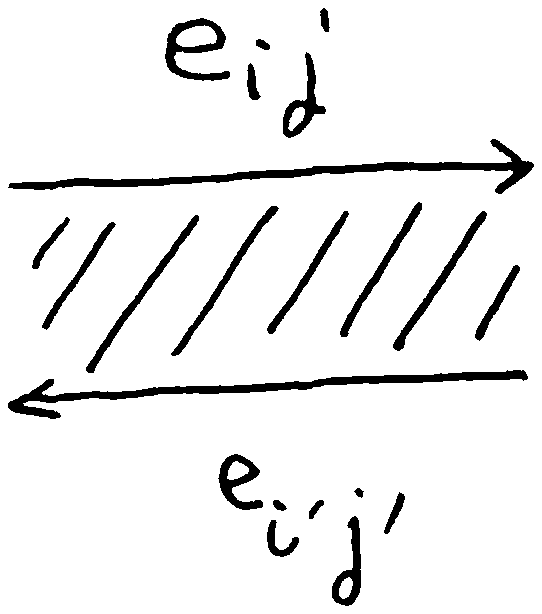
\includegraphics[width=0.24\linewidth]{fig_p33_b.png}
\end{center}

% =====================================================================
%  c04 —— PDF p.34–38（原书 p.28–32）及原书 p.33 顶端
%  §2.2 二次微分形式与带状图（续）；§2.3 具有有限模的 Riemann 面上的两个不等式
% =====================================================================

% ===== 原书 p.28 =====
此时，把$E_{i,j}\subset\overline{D}_i$定义为
\[
E_{i,j}=\Bigl\{z_i\Bigm||z_i|=1,\ \sum_{p=1}^{j-1}s_{i,p}<\frac{s_i\arg(z_i)}{2\pi i}<\sum_{p=1}^{j}s_{i,p}\Bigr\},
\]
并使用变量
\[
w_{i,j}=\frac{s_i}{2\pi i}\log(z_i)+\sum_{p=1}^{j-1}s_{i,p}.
\]
同样定义$E_{i',j'}$、$w_{i',j'}$，并由$w_{i,j}+w_{i',j'}=0$把$E_{i,j}$与$E_{i',j'}$等同。
沿图$K$粘合诸$\overline{D}_i^*$。在$\partial E_{i,j}$处也把与图顶点对应之处等同。

\begin{center}
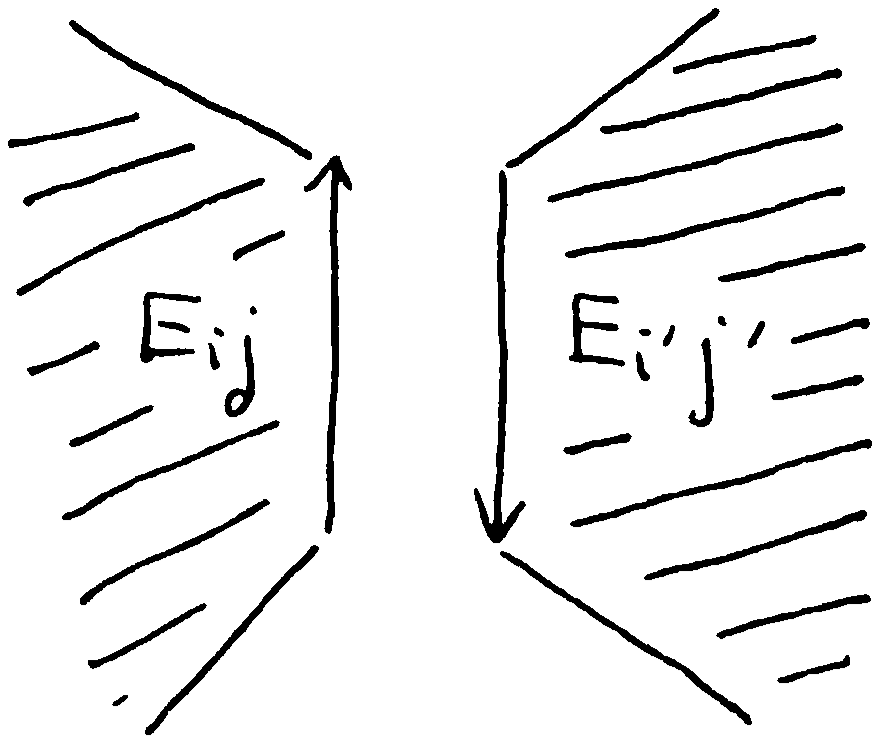
\includegraphics[width=0.40\linewidth]{fig_p34_a.png}
\end{center}

按照其顶点$v$处的价，即$\operatorname{val}(v)=\#\{e\mid v$是$e$的端点$\}$，用变量
\[
(*)\qquad u_v=w_{ij}^{\frac{2}{\overline{\operatorname{val}}(v)}}\exp\left(\frac{2\pi j\sqrt{-1}}{\operatorname{val}(v)}\right)
\]
来粘合。由此构成 r-punctured Riemann 面$(X,p_1,\dots,p_n)$。
在$\overline{D}_i^*$上用二次微分$\frac{r_i}{z_i^2}dz_i^{\otimes2}$来定义$\omega$，其中$r_i=\left(\frac{s_i}{2\pi}\right)^2$。
这一粘合得到$X$上在$p_1,\dots,p_r$有极点的二次微分，这可由
$dw_i=\frac{s_i}{2\pi i}\frac{dz_i}{z_i}$、$-dw_i^{\otimes2}=\frac{r_i}{z_i^2}dz^{\otimes2}$得知。
用坐标$u_i$在顶点$v$处表示$\omega$时，由关系$(*)$得
\[
dw^{\otimes2}=\left(\frac{\operatorname{val}(v)}{2}\right)^2u_i^{\operatorname{val}(v)-2}du_i^{\otimes2},
\]
故$\operatorname{ord}(\omega)=\operatorname{val}(v-2)$。又$\omega$在$p_i$处展开的$z_i^{-2}$的系数与$r_i$一致。
这样便构成了 Riemann 面$X$、$n$个点$p_1,\dots,p_n$及其上的二次微分$\omega$，它们满足定理 2.1 的条件。

\transnote{原文此处把点数一写作$n$、一写作$r$（「r-punctured 面$(X,p_1,\dots,p_n)$」之后紧接「$p_1,\dots,p_r$」）；照原文排印。}

\transnote{式$(*)$分母的$\operatorname{val}(v)$上多出一道上划线；照原文排印。}

\transnote{原文把$\operatorname{ord}(\omega)$印作$\operatorname{val}(v-2)$（应为$\operatorname{val}(v)-2$）；照原文排印。}

\subsection{具有有限模的 Riemann 面上的两个不等式}

Riemann 面上的有界开集$R$若含有与$R$同伦等价的$S^1$，则称之为环域。
（此处「有界」指不与$\C-\{0\}$
% ===== 原书 p.29 =====
全纯等价。）此时可知，存在唯一的$r\ge0$，使$R$与$\C$的区域$R_r=\{z\in\C\mid r<|z|<1\}$全纯等价。
$R$的模$M$由$M=-\frac{1}{2\pi}\log r$定义。此时$0<M\le\infty$。
换一种说法，$M$就是使$R_r-\R_{>0}$在$\frac{1}{2\pi i}\log(z)$下的像为
$\{x+yi\mid0<x<1,\ 0<y<M\}$的那个数。

\begin{center}
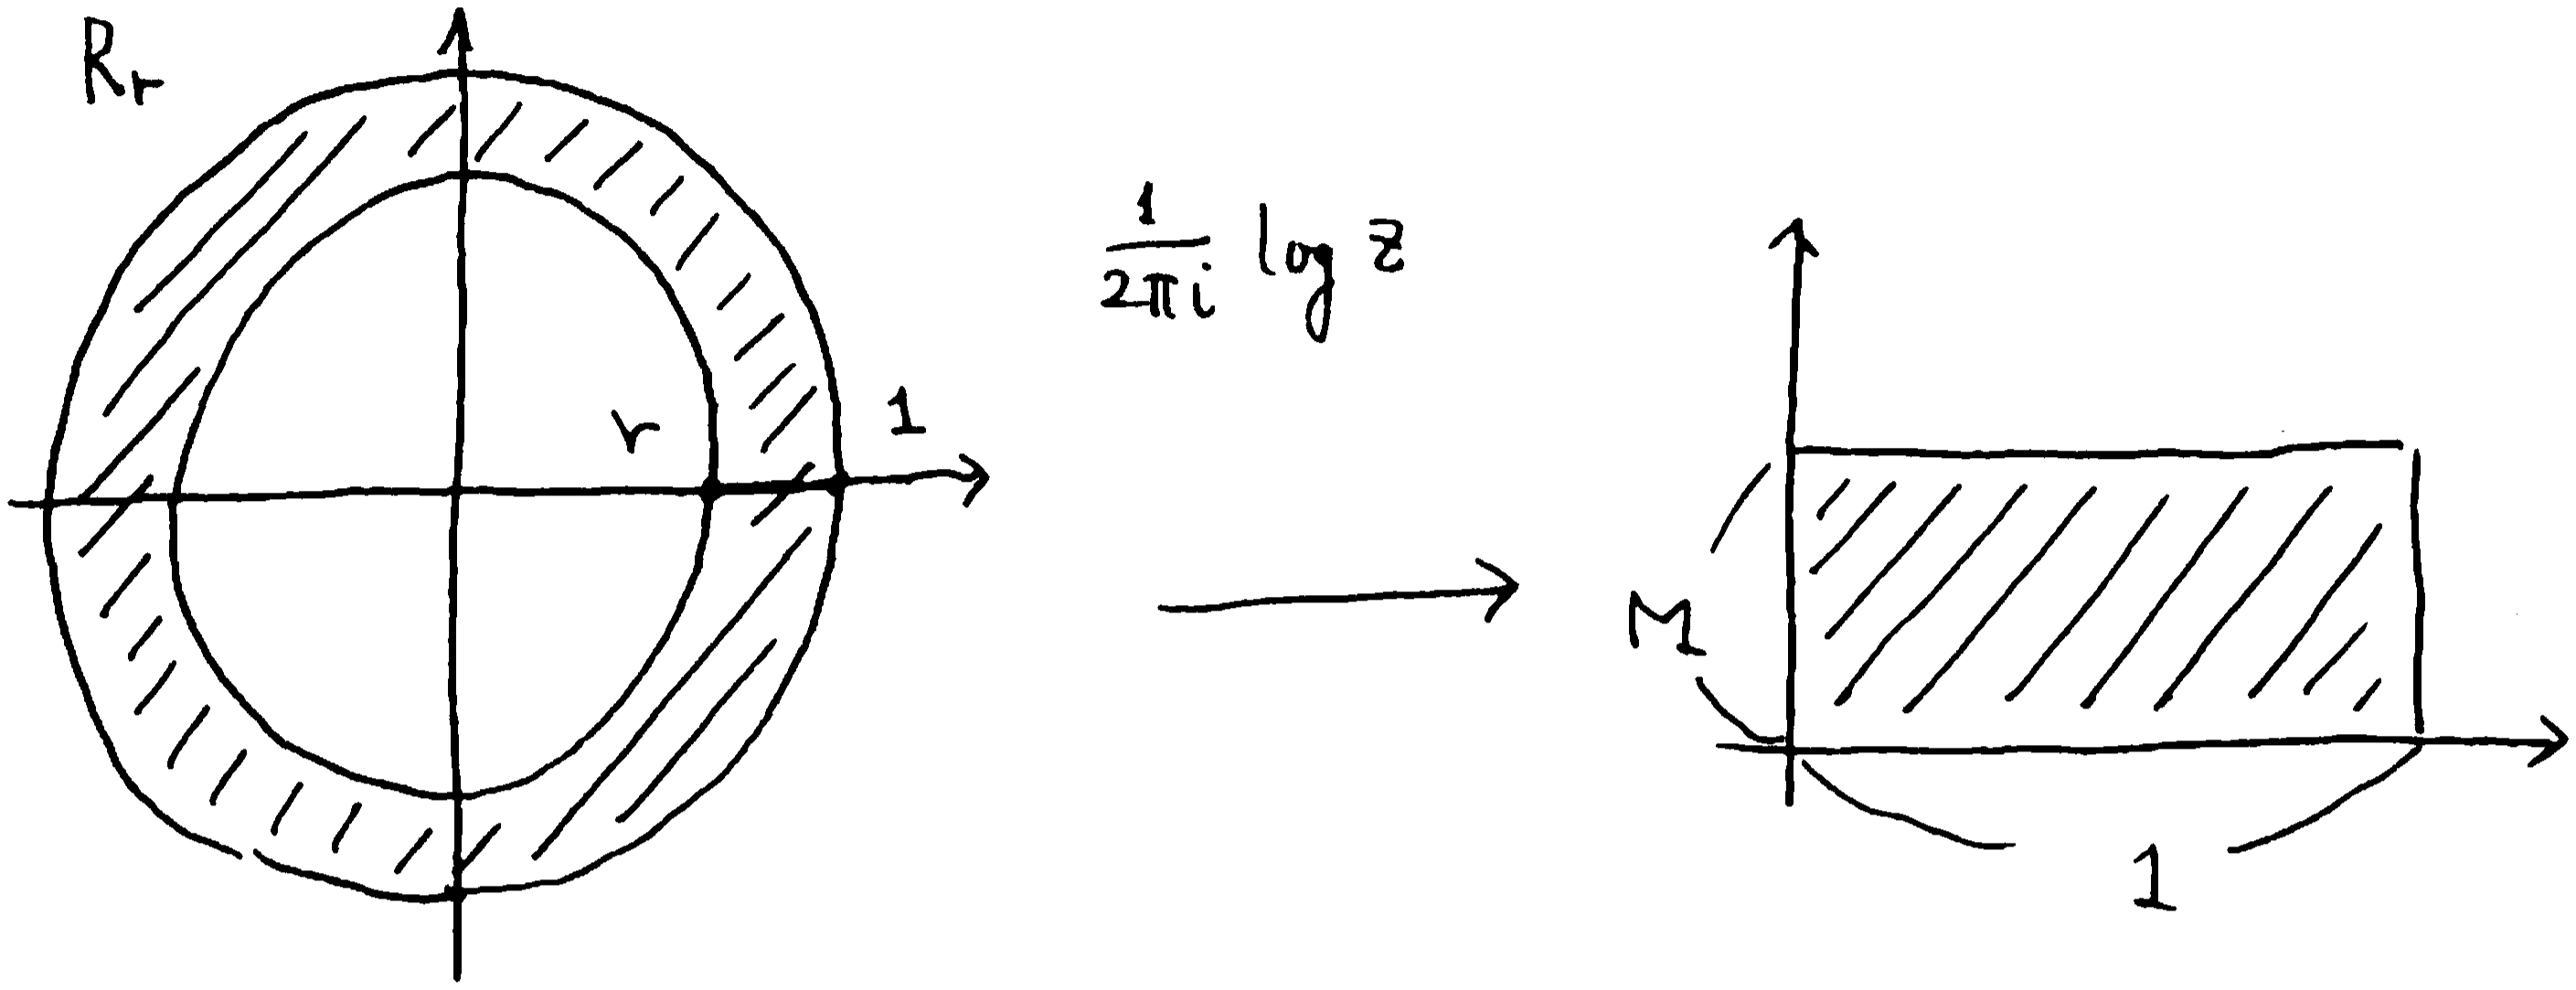
\includegraphics[width=0.88\linewidth]{fig_p35_a.png}
\end{center}

现设两个环域$R^{(1)},R^{(2)}$为有限模，且$R^{(1)}\subset R^{(2)}$，则$R^{(2)}$的模不小于$R^{(1)}$的模；
若两者一致，则$R^{(1)}=R^{(2)}$。在这个意义上，模衡量着环域的「大小」。
$D^*=\{z\mid0<|z|<1\}$的模为$\infty$，这种情形下有时也希望有计量「大小」的指标。
此时缩减模的概念就有用。设$t$为$D^*$在原点处的单值化参数。
定义$(D^*,t)$的缩减模为$\frac{1}{2\pi}\log\left|\frac{dt}{dz}(0)\right|$。
一般地，设区域$R\subset X$与$D=\{z\mid|z|<1\}$全纯等价，$p$为$R$上一点，$t$为$p$处的单值化参数。
此时$(R,p,t)$的缩减模定义为：取$\psi\colon R\xrightarrow{\ \sim\ }D$使$\psi(p)=0$，
再取$(D^*,\psi^{-1}(t))$的缩减模。
现设$R^{(1)}\subset R^{(2)}$与$D$全纯等价，$p\in R^{(1)}$，$t$为$p$处的单值化参数。
设$(R^{(i)},p,t)$的缩减模为$M_i$（$i=1,2$），则$M_1\le M_2$，等号仅在$R^{(1)}=R^{(2)}$时成立。
这样，此时也借助单值化参数$t$计量了环域的大小。

考察环域$R_r=\{z\mid r<|z|<1\}$及其上的二次微分$\omega=\frac{a^2}{z^2}dz^{\otimes2}$，
则按上节定义的$\psi(z)=\int\sqrt{\omega}$，$R_r-\R_{>0}$的像可表为
$\{x+yi\mid0<x<a,\ 0<y<aM\}$，故其面积表为$a^2M$。
这里要注意，$a$是与$R_r$同伦等价的轨道的长度。

% ===== 原书 p.30 =====
给定$X$上的二次微分$\omega$以及与$S^1$同胚的$\omega$的轨道$\gamma$（以下称之为闭轨道）时，
可知
\[
R_r=\{\gamma':\text{闭轨道}\mid\gamma'\text{与}\gamma\text{同伦}\}
\]
仍是环域。称之为$(\omega,\gamma)$对应的特征环域。
设$R_\gamma$为$(\omega,\gamma)$对应的特征环域，则与$\gamma$同伦的闭轨道$\gamma'$的长度
$a_{\gamma'}$等于$\gamma$的长度$a_\gamma$。称之为$R_\gamma$的长度。
设$R_\gamma$的模为$M_\gamma$，称$b_\gamma=a_\gamma M_\gamma$为$R_\gamma$的高。
由前面的计算，用$\omega$量出的$R_\gamma$的面积为$a_\gamma^2M_\gamma$。
若有有限个闭轨道$\gamma_1,\dots,\gamma_n$使$X-\bigcup_{i=1}^nR_{\gamma_i}$为测度$0$集，
则称$\omega$具闭轨道。此时称$(\gamma_i)_i$为闭轨道的型。
若$\omega$具闭轨道，则$X$的面积表为
\[
\|\omega\|_X=\sum_{i=1}^n a_{\gamma_i}^2M_{\gamma_i}.
\]

\transnote{原文此处的显示式印作$R_r$，而紧接的正文用$R_\gamma$；此处照原文排印。}

\begin{definition}[容许曲线系]
$X$内的简单闭曲线$\gamma_1,\dots,\gamma_n$称为容许的，指它们互不同伦，且不相交。
\end{definition}

\begin{lemma}
设$\omega$为 Riemann 面$X$上的二次微分，$\gamma_1,\dots,\gamma_n$为$X$上的容许曲线系。
设$R_i\subset X$（$i=1,\dots,n$）为互不相交且与$\gamma_i$同伦的环域。
设与$\gamma$同伦的$S^1$用$\omega$量出的长度的最小值为$a_i$，$R_i$的模为$M_i$，则
\[
\sum a_i^2M_i\le\|\omega\|_X.
\]
此外，若$\omega$具型$(\gamma_i)_i$的闭轨道，则上式中等号成立时，$R_i$与$\gamma_i$的特征环域$R_i$一致。
\end{lemma}

\transnote{原文此句用裸的$\gamma$（其余各处作$\gamma_i$），且最后一句把特征环域记作$R_i$，按文意应为$R_{\gamma_i}$；均照原文排印。}

\begin{proof}
令$r_i=\exp(-2\pi M_i)$。设$\varphi$为给出$R_i\subset X$与$R_{r_i}$全纯等价的映射，
再设它经$\frac{a_i}{2\pi i}\log\varphi(z)$把$R_{r_i}-\R_{>0}$映入长方形$S_i$，
则在此映射下由$\omega$决定的度量为$\rho(x,y)\sqrt{dx^2+dy^2}$。
又该长方形的高可用模$M_i$写成$b_i=a_iM_i$。现对$0<\mu<b_i$的$\mu$，
% ===== 原书 p.31 =====
$S_i$内的直线$(\R+\mu\sqrt{-1})\cap S_i$用$\rho(x,y)\sqrt{dx^2+dy^2}$量出的长度不超过$a_i$。
\[
a_i\le\int_0^{a_i}\rho(x+iy)dx\qquad(0\le y\le b_i)
\]
再对$y$从$0$到$b_i$积分，得
\[
a_ib_i\le\int_{S_i}\rho(x,y)dxdy.
\]
因此
\[
\sum_{i=1}^n a_ib_i\le\sum_{i=1}^n\int_{S_i}\rho(x,y)dxdy.
\]
用 Schwartz 不等式，
\begin{align*}
\left(\sum_{i=1}^n a_ib_i\right)^2
&\le\left(\sum_{i=1}^n\int_{S_i}\rho(x,y)dxdy\right)^2\\
&\le\left(\sum_{i=1}^n a_ib_i\right)
  \left(\sum_{i=1}^n\frac{1}{a_ib_i}\left(\int_{S_i}\rho(x,y)dxdy\right)^2\right)\\
&\le\left(\sum_{i=1}^n a_ib_i\right)
  \left(\sum_{i=1}^n\int_{S_i}\rho(x,y)^2dxdy\right).
\end{align*}
因$\int_{S_i}\rho(x,y)^2dxdy=\|\omega\|_{S_i}$，故
\[
\sum_{i=1}^n a_ib_i\le\sum_{i=1}^n\|\omega\|_{S_i}\le\|\omega\|_X.
\]

\transnote{原书把 Schwarz 拼作 Schwartz；照原文排印。}
后半部分的证明如下。若$\omega$具型$(\gamma_i)_i$的闭轨道，则$a_i$为$\gamma_i$的长度。
上面等号成立意味着向量$(\sqrt{a_i,b_i})_i$与
$\left(\frac{1}{\sqrt{a_ib_i}}\int_{S_i}\rho\,dxdy\right)_i$平行，且$\rho$为常函数。
由此可知，证明开头所定义的$\frac{a_i}{2\pi i}\log\varphi$
与由二次微分$\omega$决定的$\psi(z)=\int\sqrt{\omega}$只相差一个常数倍。
该常数为实数，这一点由叶状结构的样子可知。
因此，$R_i$与$\omega$对应的$\gamma_i$的特征环域一致。
\end{proof}

\transnote{原文把向量印作$(\sqrt{a_i,b_i})_i$，多出一个逗号（应为$\sqrt{a_ib_i}$）；照原文排印。}

现设$X$为紧 Riemann 面，$p_1,\dots,p_n$为其上的$n$个点，$\omega$为二次微分。
挖去$p_i$周围的小圆盘$D_i$所得的 Riemann 面$\tilde X=X-\bigcup_{i=1}^nD_i$上，
关于由$\omega$决定的度量的面积有限。
由此，对任意的闭曲线$\gamma_i\subset X$，$\{M_i\mid M_i$为与$\gamma$同伦等价的环域的模$\}$有界。

试就缩减模考虑引理 2.2。

% ===== 原书 p.32 =====
\begin{lemma}
设$X$为紧 Riemann 面，$p_1,\dots,p_n$为$X$上的$n$个点，$z_1,\dots,z_n$为$p_1,\dots,p_n$处的单值化参数。
设$\omega$为二次微分，它具以绕$p_1,\dots,p_n$的小闭曲线$\gamma_1,\dots,\gamma_n$为型的闭轨道。
现设存在以$p_i$为 puncture、互不相交的环域$R_i'$，设$M_i'$为其缩减模，则
\[
\sum_{i=1}^n a_i^2M_i'\le\sum_{i=1}^n a_i^2M_i.
\]
其中$M_i$为$\gamma_i$的特征环域关于$z_i$的缩减模，$a_i$为其长度。
又若等号成立，则$R_i=R_i'$。
\end{lemma}

\begin{proof}
首先设把$R_i'$移到$D^*=\{z\in\C\mid0<|z|<1\}$的全纯同构为$\varphi_i$。令
$D_i(\varepsilon)=\{z\in R_i'\mid|\varphi_i(z)|\le\varepsilon\}$，
$R_i'(\varepsilon)=R_i'-D_i(\varepsilon)$，$R_i(\varepsilon)=R_i-D_i(\varepsilon)$，
$X(\varepsilon)=X-\bigcup_{i=1}^nD_i(\varepsilon)$。
与引理 2.2 证明的前半部分相同，若$|\varphi_i(x)|=\mathrm{const}\ge\varepsilon$中存在非闭轨道者，
则存在$\delta>0$使
\[
\sum_{i=1}^n a_i^2M_i'(\varepsilon)+\delta\le\|\omega\|_{X(\varepsilon)}.
\]
两边加上$\sum_{i=1}^n\frac{a_i}{2\pi i}\log(\varepsilon)$，并令$\varepsilon\to0$。此时
\[
M_i'(\varepsilon)+\frac{1}{2\pi i}a_i^2\log(\varepsilon)=M_i',\qquad
\lim_{\varepsilon\to\infty}\left(M_i(\varepsilon)+\frac{a_i}{2\pi}\log(\varepsilon)\right)=M_i
\]
以及$\|\omega\|_{X(\varepsilon)}-\sum_{i=1}^nM_i(\varepsilon)\to0$，故得
\[
\sum_{i=1}^n a_i^2M_i'+\delta\le\sum_{i=1}^n a_i^2M_i.
\]
即使$|\varphi(z)|=\mathrm{const}$全为闭轨道，上面的不等式也以$\delta=0$成立。
又等号成立时，$\omega$在$X(\varepsilon)$上的限制为具闭轨道的二次微分，
故由引理的后半部分得$R_i(\varepsilon)=R_i'(\varepsilon)$。由此得$R_i=R_i'$。
\end{proof}

\transnote{原文此处印作$\lim_{\varepsilon\to\infty}$，按上下文应为$\varepsilon\to0$；照原文排印。}

迄今处理了关于长度与模的不等式，下面考察关于高与模的不等式。

\begin{theorem}
设$\omega$为具型$(\gamma_i)_i$的闭轨道、且$\|\omega\|_X<\infty$的二次微分。
设$R_i'$为互不相交的、与$\gamma_i$同伦等价的环域，
% ===== 原书 p.33 =====
% （本页只取定理 2.4 陈述的末段；证明由下一块承译。）
$M_i'$为其模，则
\[
\sum_{i=1}^n\frac{b_i}{M_i}\le\sum_{i=1}^n\frac{b_i}{M_i'}.
\]
其中$M_i$、$b_i$为$\gamma_i$对应的特征环域$R_i$的模与高。
又等号成立时，$R_i=R_i'$。
\end{theorem}

% =====================================================================
%  c05 —— PDF p.39–45（原书 p.33–39）
%  §2.4 二次微分的存在定理
% =====================================================================

% ===== 原书 p.33 =====
% （本页开头承接上一块：定理 2.4 陈述的末段，由 c04 译完，此处跳过；
%   以下从本页开始的定理 2.4 的证明起译。）

\begin{proof}
设$a_i$为$R_i$的长度，$\varphi$为把$R_i'$映到$R=\{z\mid\exp(-2\pi iM_i')<|z|<1\}$的正则映射。再考虑$\frac{b_i}{2\pi iM_i}\log(\varphi)$，它把$R_i'$映到$S_i'=\{x+iy\mid0<x<\tilde a_i,\ 0<y<b_i\}$，其中$\tilde a_i=\frac{b_i}{M_i}$。这里写成$|\sqrt{\omega}|=\rho(x,y)\sqrt{dx^2+dy^2}$时，由
\[
a_i\le\int_0^{\tilde a_i}\rho(x,y)\,dx
\]
得
\[
a_ib_i\le\int_{S_i'}\rho(x,y)\,dx\,dy,\qquad
\sum_{i=1}^n a_ib_i\le\sum_{i=1}^n\int_{S_i'}\rho(x,y)\,dx\,dy.
\]
因此
\[
\begin{aligned}
\left(\sum_{i=1}^n a_ib_i\right)^2
&\le\left(\sum_{i=1}^n\int_{S_i'}\rho(x,y)\,dx\,dy\right)^2\\
&\le\left(\sum_{i=1}^n\tilde a_ib_i\right)
 \left(\sum_{i=1}^n\frac{1}{\tilde a_ib_i}
 \left(\int_{S_i}\rho(x,y)\,dx\,dy\right)^2\right)\\
&\le\left(\sum_{i=1}^n\tilde a_ib_i\right)
 \left(\sum_{i=1}^n\frac{1}{\tilde a_ib_i}
 \int_{S_i}\rho^2(x,y)\,dx\,dy\cdot\tilde a_ib_i\right)\\
&=\left(\sum_{i=1}^n\tilde a_ib_i\right)
 \left(\sum_{i=1}^n\int_{S_i}\rho^2(x,y)\,dx\,dy\right)\\
&\le\left(\sum_{i=1}^n\tilde a_ib_i\right)
 \left(\sum_{i=1}^n a_ib_i\right).
\end{aligned}
\]
由此得到$\sum_{i=1}^n a_ib_i\le\sum_{i=1}^n\tilde a_ib_i$。等号的情形与引理 2.2 相同，故省略。
\end{proof}

\transnote{原书 p.33 的证明开头把环域写作$\exp(-2\pi iM_i')<|z|<1$，把映射的分母写作$2\pi iM_i$；其中$i$的用法以及$M_i$与$M_i'$的搭配疑有笔误，此处照原文译出。}

\subsection{二次微分的存在定理}

\begin{theorem}
设$X$为 Riemann 面，$\gamma_1,\dots,\gamma_n$为可容许（admissible）的曲线系。假设条件
% ===== 原书 p.34 =====
\begin{itemize}[leftmargin=3.2em,itemsep=2pt,topsep=4pt]
\item[(fin)] 集合$\{M_i\mid M_i$为与$\gamma_i$同伦等价的环域$R_i$的模$\}$有界
\end{itemize}
成立。则对$\R_+$中任意元素$b_1,\dots,b_n$，存在唯一的二次微分$\omega$，它具有类型$(\gamma_i)_i$的闭轨道，且以$b_1,\dots,b_n$为特征环域（characteristic ring domain）的高度。
\end{theorem}

\begin{proof}
取互不相交的类型$(\gamma_i)_i$的环域$(R_{ip})$（$p=1,2,\dots$），设$M_{ip}$为$R_{ip}$的模，并使$\sum_{i=1}^n\frac{b_i^2}{M_{ip}}$成为趋于其下确界的序列。因$M_i$有界，故必要时取其部分列，可设$\lim_{p\to\infty}M_{ip}=M_i$存在。设$g_{in}$为从$D_{in}=\{\exp(-2\pi M_{in})<|z|<1\}$到$R_{in}$的正则同构，则利用正规族的论述，作为$\{g_{in}\}_n$的某个部分列的极限，存在从$D_i=\{\exp(-2\pi M_i)<|z|<1\}$到$X$的函数$g_i$；其像$R_i$为互不相交的类型$(\gamma_i)_i$的环域，且$\sum_{i=1}^n\frac{b_i^2}{M_i}$达到前面出现的下确界。

现考虑与 id 充分「接近」的$C^\infty$-map $F\colon R\to R$。（所谓「接近」，后面会明白。）记$\tilde R_i=F(R_i)$，$R_i,\tilde R_i$的模分别为$M_i,\tilde M_i$。设$R_i,\tilde R_i$与$D_{M_i},D_{\tilde M_i}$的同构为$\varphi,\tilde\varphi_i$，$a_i=\frac{b_i}{M_i}$，$\tilde a_i=\frac{b_i}{\tilde M_i}$。这里$D_M=\{z\in\C\mid\exp(-2\pi M)<|z|<1\}$。

\transnote{原文把 $C^\infty$ 映射写作「$C^\infty$-map」（原书 p.34），下文（原书 p.35）亦同；译本照原文保留该写法，不改为「映射」。}

再令$\zeta=\frac{a_i}{2\pi i}\log\varphi_i$，$f(\zeta)=\frac{\tilde a_i}{2\pi i}\log\tilde\varphi_i$。此时作为$\zeta$的函数，$f(\zeta)$只能确定到相差$2\pi i\Z$，但$f_\zeta=\frac{df}{d\zeta}$、$f_{\bar\zeta}=\frac{df}{d\bar\zeta}$确定；由$\zeta=\xi+i(\text{const.})$确定的曲线族经$f$的像的长度，可用$\int|f_\zeta+f_{\bar\zeta}|\,d\xi$计算。因此
\[
\tilde a_i\le\int|f_\zeta+f_{\bar\zeta}|\,d\xi
\]
成立。令$\zeta=\xi+\eta i$，在$S_i$上进行上面的积分，则
\[
\begin{aligned}
\tilde a_ib_i&\le\int_{S_i}|f_\zeta+f_{\bar\zeta}|\,d\xi\,d\eta\\
&=\int J(f)^{\frac12}\,\frac{|f_\zeta+f_{\bar\zeta}|}{J(f)^{\frac12}}\,d\xi\,d\eta
\end{aligned}
\]
成立。这里利用$J(f)=|f_\zeta|^2-|f_{\bar\zeta}|^2$，由 Schwarz 不等式得
\[
\begin{aligned}
(\tilde a_ib_i)^2&\le\int_{S_i}J\,d\xi\,d\eta\int_{S_i}
 \frac{|f_\zeta+f_{\bar\zeta}|^2}{|f_\zeta|^2-|f_{\bar\zeta}|^2}\,d\xi\,d\eta\\
&=\tilde a_ib_i\int_{S_i}\frac{|1+\kappa|^2}{1-|\kappa|^2}\,d\xi\,d\eta.
\end{aligned}
\]

% ===== 原书 p.35 =====
这里$\kappa=f_{\bar\zeta}/f_\zeta$，是称为伸缩率（dilatation）的数。因此
\[
\frac{b_i^2}{\tilde M_i}\le\int_{S_i}\frac{|1+\kappa|^2}{1-|\kappa|^2}\,d\xi\,d\eta\qquad(\ast)
\]
成立。

现设$U$为$X$的充分小的开集，$z=x+yi$为$U$上的复坐标。又设$h(z)$为$U$上具有充分小支集的$C^\infty$函数。此时对充分小的$\epsilon$，$F\colon z\mapsto z+\epsilon h(z)$是$U$上的微分同胚，并在$U$以外延拓为 id。令$U_i=U\cap R_i$，就这个$F$执行$(\ast)$的积分。设$\Phi_i=\frac{a_i}{2\pi i}\log\varphi_i\colon R_i\to S_i$，$W_i$为对应于$U_i$的开集，注意在$S_i-W_i$上为 id 且$\kappa=0$，则
\[
\begin{aligned}
\int_{S_i}\frac{|1+\kappa|^2}{1-|\kappa|^2}\,d\xi\,d\eta
&=\int_{S_i-W_i}d\xi\,d\eta+\int_{W_i}\frac{|1+\kappa|^2}{1-|\kappa|^2}\,d\xi\,d\eta\\
(\ast\ast)\qquad
&=\int_{S_i-W_i}d\xi\,d\eta+\int_{U_i}\frac{|1+\kappa|^2}{1-|\kappa|^2}
 \left|\frac{d}{dz}\Phi_i\right|^2dx\,dy
\end{aligned}
\]
成立。

第2项的积分要用伸缩率的性质。一般地，伸缩率$\kappa$是对复区域$D_1,D_2$、与共形等价充分接近的$C^\infty$-map $f\colon D_1\to D_2$、以及$D_1,D_2$的单值化参数（uniformizer）$z_1,z_2$定义的量，由
\[
\kappa=\kappa(f,z_1,z_2)
=\left(\frac{\partial(z_2\circ f)}{\partial\bar z_1}\right)
\Big/\left(\frac{\partial(z_2\circ f)}{\partial z_1}\right)
\]
定义。容易看出，它不依赖于$D_2$的单值化参数$z_2$。又容易看出，把$z_1$换成别的单值化参数$z_1'$时，令$\tau=\frac{dz_1'}{dz_1}$，有
\[
\kappa(f,z_1',z_2)=\kappa(f,z_1,z_2)\cdot\frac{\tau}{\bar\tau}
\]
成立。上面给出的$F$关于$z$坐标的伸缩率为$\frac{\epsilon h_{\bar z}(z)}{1+\epsilon h_z(z)}$，故关于$\zeta$的伸缩率为
\[
\frac{\epsilon h_{\bar z}(z)}{1+\epsilon h_z(z)}
\cdot\frac{\left(\frac{d}{dz}\Phi_i\right)^2}
{\left|\frac{d}{dz}\Phi_i\right|^2}.
\]
$(\ast\ast)$第2项的被积函数在模$O(\epsilon^2)$的意义下等于
\[
\begin{aligned}
\frac{|1+\kappa|^2}{1-|\kappa|^2}\left|\frac{d}{dz}\Phi_i\right|^2
&=|1+\kappa|^2\left|\frac{d}{dz}\Phi_i\right|^2+O(\epsilon^2)\\
&=(1+2\Re(\kappa))\left|\frac{d}{dz}\Phi_i\right|^2+O(\epsilon^2)\\
&=\left|\frac{d}{dz}\Phi_i\right|^2
 +2\epsilon\Re\left(h_{\bar z}\left(\frac{d}{dz}\Phi_i\right)^2\right)+O(\epsilon^2).
\end{aligned}
\]

% ===== 原书 p.36 =====
因此$(\ast\ast)$的积分等于
\[
a_ib_i+2\epsilon\Re\int_{U_i}h_{\bar z}
\left(\frac{d}{dz}\Phi_i\right)dx\,dy+O(\epsilon^2)\text{。}
\]
由此
\[
\begin{aligned}
\sum_{i=1}^n a_ib_i&\le\sum_{i=1}^n\tilde a_ib_i\\
&\le\sum_{i=1}^n\left(a_ib_i+2\epsilon\Re\int_{U_i}h_{\bar z}
 \left(\frac{d}{dz}\Phi_i\right)^2dx\,dy\right)+O(\epsilon^2).
\end{aligned}
\]
由于充分小的$\epsilon$可任意变动，
\[
\sum\Re\int_{U_i}h_{\bar z}
\left(\frac{d}{dz}\Phi_i\right)^2dx\,dy=0
\]
成立。

$h_{\bar z}$是具有充分小支集的任意$C^\infty$函数，故把各$U_i$上的$\left(\frac{d}{dz}\Phi_i\right)^2$粘贴所得的函数，作为广义函数看时关于$\bar z$的微分为$0$。因此它与$U$上某个全纯函数除一个零测集外一致。由此$\left(\frac{d}{dz}\Phi_i\right)^2dz^{\otimes2}$定义了$X$上的全纯二次微分。对应的特征环域为$R_i$。唯一性由定理 2.4 推出。
\end{proof}

\begin{remark}
用现在的方法，由$(b_1,\dots,b_n)$唯一确定$(M_1,\dots,M_n)$，但已知这个对应是连续的（Strebel）。后文也要用这个事实，证明省略。
\end{remark}

下面考察给定模时的情形。设给定 Riemann 面$X$与曲线的可容许系$\gamma_1,\dots,\gamma_n$，且定理 2.5 的条件 (fin) 满足。此时令
\[
\mathcal{H}=\Bigl\{(b_1^2,\dots,b_n^2)\ \Bigm|
\begin{array}{l}
\text{$X$上存在二次微分$\omega$，它满足$\|\omega\|_X=1$，具有类型$(\gamma_i)_i$的闭轨道，}\\[1pt]
\text{且关于$\gamma_1,\dots,\gamma_n$的特征环域的高度为$b_1,\dots,b_n$}
\end{array}\Bigr\}.
\]
称之为高度曲面（height surface）。现对$e=(e_1,\dots,e_n)$，$\sum e_i^2=1$，$e_i>0$，存在唯一的$\lambda>0$使$\lambda e\in\mathcal{H}$。事实上，取具有类型$(\gamma_i)_i$的闭轨道、对应特征环域的高度为$\sqrt{e_1},\dots,\sqrt{e_n}$的二次微分$\omega'$，令$\omega=\omega'/\|\omega'\|_X$，其高度记为$b_1,\dots,b_n$，则$(b_1^2,\dots,b_n^2)\in\mathcal{H}$，且
\[
(b_1^2,\dots,b_n^2)=(e_1,\dots,e_n)\cdot\|\omega'\|_X^{-2}
\]
成立。

% ===== 原书 p.37 =====
又由定理 2.5 的唯一性，若$\omega^{(1)},\omega^{(2)}$都具有类型$(\gamma_i)_i$的闭轨道，其特征环域的高度分别为$(b_1^{(1)},\dots,b_n^{(1)})$、$(b_1^{(2)},\dots,b_n^{(2)})$，且$\mu(b_1^{(1)},\dots,b_n^{(1)})=(b_1^{(2)},\dots,b_n^{(2)})$，则$\mu\omega^{(1)}=\omega^{(2)}$。在$\|\omega^{(1)}\|_X=\|\omega^{(2)}\|_X$的假设下，$\mu=1$，从而$\R_+e\cap\mathcal{H}$只有一点。

\begin{lemma}
$\mathcal{H}\subset\R^n$是严格凸的，在点$(x_1,\dots,x_n)=(b_1^2,\dots,b_n^2)$处的切平面由
\[
\frac{x_1}{M_1}+\cdots+\frac{x_n}{M_n}=1
\]
给出。这里$(M_1,\dots,M_n)$为对应于$(b_1^2,\dots,b_n^2)$的二次微分$\omega$的特征环域的模。
\end{lemma}

\begin{proof}
设$\tilde\omega$为具有类型$(\gamma_i)_i$的闭轨道、满足$\|\tilde\omega\|_X=1$、且其特征环域的高度为$\tilde b_1,\dots,\tilde b_n$的二次微分。此时只需证明
\[
\frac{\tilde b_1^2}{M_1}+\cdots+\frac{\tilde b_n^2}{M_n}\ge1.
\]
这是因为：当互不相交的类型$(\gamma_i)_i$的环域的模$m_i$变动时，使$\frac{\tilde b_1^2}{m_1}+\cdots+\frac{\tilde b_n^2}{m_n}$达到最小值的$(m_1,\dots,m_n)$，正是$\tilde\omega$的特征环域$\tilde R_i$的模$\tilde M_1,\dots,\tilde M_n$，故
\[
\frac{\tilde b_1^2}{M_1}+\cdots+\frac{\tilde b_n^2}{M_n}
\ge\frac{\tilde b_1^2}{\tilde M_1}+\cdots+\frac{\tilde b_n^2}{\tilde M_n}=1
\]
成立。又当等号成立时，令$R_i$为$\omega$的特征环域，则$\tilde R_i=R_i$。这意味着$\mathcal{H}$是严格凸的。
\end{proof}

\begin{center}
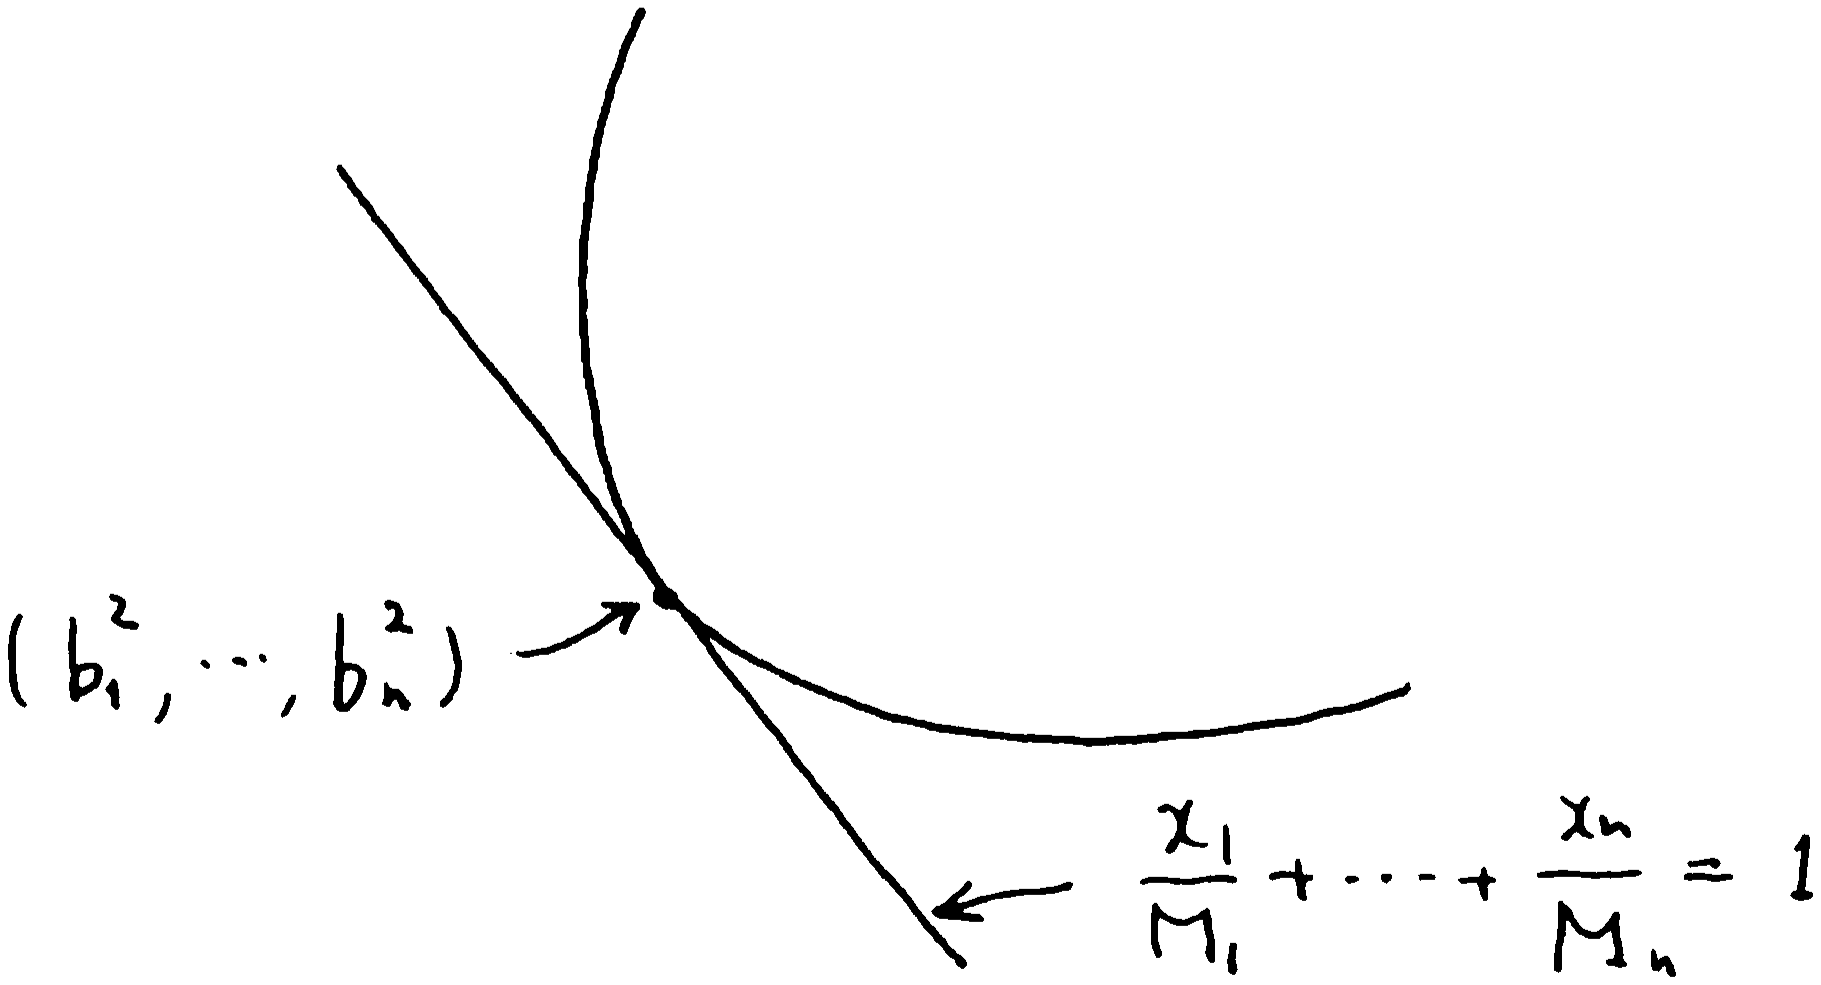
\includegraphics[width=0.5\linewidth]{fig_p43_a.png}
\end{center}

下面看看$\mathcal{H}$的边界上的情形。

% ===== 原书 p.38 =====
\begin{lemma}
\begin{enumerate}[label=(\arabic*)]
\item $\mathcal{H}$是有界集合。
\item 对$1\le i\le n$，考虑$\{x_i=0\}\cap\bar{\mathcal{H}}$。则对任意的
$e=(e_1,\dots,\check{0},\dots,e_n)$，$e_1^2+\cdots+e_n^2=1$，$e_i>0$，
存在某个$\lambda$使$\lambda e\in\{x_i=0\}\cap\bar{\mathcal{H}}$，
且该处的切平面的法向量由$(0,\dots,\check{1},\dots,0)$给出。
这里$\bar{\mathcal{H}}$是$\mathcal{H}$在$\R^n$内的闭包。
\end{enumerate}
\end{lemma}

\begin{proof}
(1) 由$\frac{\tilde b_1^2}{M_1}+\cdots+\frac{\tilde b_n^2}{M_n}=1$得$b_1^2\le M_1$，再由条件 (fin) 知有界。

(2) 考虑$b_i\to0$的极限，对$\gamma_1,\dots,\check{\gamma}_i,\dots,\gamma_n$考虑求高度为$b_1,\dots,\check{b}_i,\dots,b_n$的二次微分的问题，可知$M_i\to0$。切平面的法向量
\[
\left(\frac{1}{M_1},\dots,\frac{\check{1}}{M_i},\dots,\frac{1}{M_n}\right)
\Big/\sqrt{\sum_{i=1}^nM_i^{-2}}
\]
收敛于$e_i$。
\end{proof}

\transnote{原书 p.38 引理 2.7 的证明 (1) 处印作$b_1^2\le M_1$（只带下标$1$），据上下文应为$b_i^2\le M_i$；此处照原文印出。}

下面证明给定模（之比）时二次微分的存在性。

\begin{theorem}
设$X,(\gamma_i)_i$与定理中相同，并假设条件 (fin) 成立。给定$m=(m_1,\dots,m_n)\in\R_+^n$时，存在唯一的二次微分$\omega$，它满足$\|\omega\|_X=1$，具有类型$(\gamma_i)_i$的闭轨道，且其模$M_1,\dots,M_n$满足$(M_1,\dots,M_n)=\lambda(m_1,\dots,m_n)$（$\lambda>0$）。
\end{theorem}

\transnote{原书定理 2.8 的陈述只说「与 Theorem 相同」，未标编号，据前后文当指定理 2.5；此处照原文译出。}

\begin{proof}
令$e=(m_1,\dots,m_n)/\sqrt{\sum m_i^2}=(e_1,\dots,e_n)$，$c=\min\{x_1e_1+\cdots+x_ne_n\mid(x_1,\dots,x_n)\in\bar{\mathcal{H}}\}$。证明达到这个最小值的$(x_1,\dots,x_n)$属于$\R_+^n$。若不然，设$x=(t_1,\dots,\check{0},\dots,t_n)$，且这个$c$被达到。过此点、以$e$为法向量的平面为$e_1(x_1-t_1)+\cdots+e_ix_i+\cdots+e_n(x_n-t_n)=0$。若$(y_1,\dots,y_n)\in\bar{\mathcal{H}}$，则必须有$e_1(y_1-t_1)+\cdots+e_iy_i+\cdots+e_n(y_n-t_n)\ge0$。考虑满足$(y_1,\dots,\check{0},\dots,y_n)=\tau(t_1,\dots,t_n)$且$y_i\to t_i$的情形，则$(y_1-t_1:\cdots:y_i:\cdots:y_n-t_n)$收敛于与$e_i$正交的方向，因此$\frac{y_i}{1-\tau}\to0$。此时
\[
e_1(y_1-t_1)+\cdots+e_iy_i+\cdots+e_n(y_n-t_n)
=(\tau-1)e_1t_1+\cdots+e_iy_i+\cdots+(\tau-1)e_nt_n,
\]
故存在某个$(y_1,\dots,y_n)$使上式为负。这与前面矛盾。

% ===== 原书 p.39 =====
又，$c$的值在两个以上坐标变为$0$的点处被达到的情形也同样可证。（注意，思考其意义可知，把$\bar{\mathcal{H}}$限制到$x_i=0$上正是关于$\gamma_1,\dots,\check{\gamma}_i,\dots,\gamma_n$的高度曲面，因此考察只有一个坐标变为$0$的情形就足够了。）
\end{proof}

% =====================================================================
%  c06 —— PDF p.46–54（原书 p.40–48）
%  §3 Moduli stack 的相交理论；§3.1 由粘合构造叠
%  说明：交换图均用 tikz-cd 重画（原书图幅小、字密，裁图后放大即模糊）。
% =====================================================================

% ===== 原书 p.40 =====
\section{Moduli stack 的相交理论}

\subsection{由粘合构造叠}

为了用二次微分（quadratic differential）定义代数叠（algebraic stack）或与之相伴的解析叠（analytic stack）的胞腔分解，这里把叠实现为余等化子（coequalizer）。

设$C$为带 Grothendieck 拓扑$E$的范畴，$S$为$(C,E)$上的叠。$F:S\to C$为$S$的结构态射。$S$为$E$-叠，是指存在可表的叠$X_0$及$E$-满射的态射$\pi_0:X_0\to S$，且$S\to S\times_CS$可表。当$C$为$\C$上的代数簇、$E$为平展拓扑时，这无非是$\C$代数叠。由$\pi_0$的可表性，$X_1=X_0\times_SX_0$再次可表。令$pr_i:X_1=X_0\times_SX_0\to X_0$为自然投影，$\Delta:X_0\to X_1$为对角态射。

一般地，在范畴$C$中，两个对象$X_0,X_1$及三个态射$pr_1,pr_2:X_1\to X_0$、$\Delta:X_0\to X_1$的组合若满足$pr_1\circ\Delta=pr_2\circ\Delta=\id_{X_0}$，则称为$C$的 1-单纯对象（1-simplicial object），记作$X_1\rightrightarrows X_0$。进一步，1-单纯对象$X_1\rightrightarrows X_0$称为对称的，是指存在对合$\theta:X_1\to X_1$满足$pr_1=pr_2\circ\theta$。给定 1-单纯对象$X_1\rightrightarrows X_0$及$X_0$上的对象$a_0:Y\to X_0$时，若写$X_1\times_{X_0}Y$，除非另有说明，都表示把$X_1$经由$pr_2$看作$X_0$上的对象；若写$Y\times_{X_0}X_1$，则表示把$X_1$经由$pr_1$看作$X_0$上的对象。

$X_0$上的对象$Y$称为带下降数据（descent data），是指给定同构$\psi:X_1\times_{X_0}Y\to Y\times_{X_0}X_1$，且下图可换。
\begin{center}
\begin{tikzcd}[column sep=3.6em, row sep=2.8em]
X_1\times_{X_0}Y \arrow[r, "\psi"'] \arrow[d, "pr_1"'] & Y\times_{X_0}X_1 \arrow[d, "pr_2"]\\
X_1 \arrow[r, "\simeq"] & X_1
\end{tikzcd}
\end{center}

% ===== 原书 p.41 =====
下降数据称为满足上闭链条件（cocycle condition），是指下图可换。
\begin{center}
\begin{tikzcd}[column sep=4em, row sep=3.4em]
X_1\times_{X_0}X_1\times_{X_0}Y \arrow[r, "pr_{23}^*(\psi)"] \arrow[d, equal] & X_1\times_{X_0}Y\times_{X_0}X_1 \arrow[d, "pr_{12}^*(\psi)"]\\
X_1\times_{X_0}X_1\times_{X_0}Y \arrow[r, "pr_{13}^*(\psi)"] & Y\times_{X_0}X_1\times_{X_0}X_1
\end{tikzcd}
\end{center}

又，若给定$C$的对象$Y,\tilde Y,X_0$及三个态射$a_\#:\tilde Y\to Y$，$a_0:\tilde Y\to X_0$，则称$\tilde Y$为$(Y,X_0)$-双对象（biobject）。$(Y,X_0)$-双对象的平凡化（trivialization），是指同构$a_1:\tilde Y\times_Y\tilde Y\cong\tilde Y\times_{X_0}X_1$，且下图可换。
\begin{center}
\begin{tikzcd}[column sep=2.6em, row sep=3em]
\tilde Y & \tilde Y\times_Y\tilde Y \arrow[l, "pr_1"'] \arrow[r, "a_0\circ pr_2"] \arrow[d, "a_1"] & X_0\\
\tilde Y \arrow[u, equal] & \tilde Y\times_{X_0}X_1 \arrow[l, "pr_1"'] \arrow[r, "pr_2\circ pr_2"] & X_0 \arrow[u, equal]
\end{tikzcd}
\end{center}
以及下图也可换。
\begin{center}
\begin{tikzcd}[column sep=3.6em, row sep=2.8em]
\tilde Y\times_Y\tilde Y \arrow[r, "\theta_{\tilde Y}"'] \arrow[d] & \tilde Y\times_Y\tilde Y \arrow[d]\\
X_1 \arrow[r, "\theta"'] & X_1
\end{tikzcd}
\end{center}

此时，态射的合成
\[
X_1\times_{X_0}\tilde Y\xrightarrow{\theta\times1}\tilde Y\times_{X_0}X_1\xleftarrow{a_1}\tilde Y\times_Y\tilde Y\xrightarrow{\theta_{\tilde Y}}\tilde Y\times_Y\tilde Y\xrightarrow{a_1}Y\times_{X_0}X_1
\]
给出下降数据。它满足上闭链条件时，称此平凡化满足上闭链条件。又，取上述的$Y$为$X_0$的情形，把$X_1$经由$pr_1$看作$X_0=Y$上的对象，再经由$pr_2$赋予$a_0$-结构，则$X_1$可看作$(X_0,X_0)$-双对象。此时的平凡化$\psi:X_1\times_{pr_2,X_0,pr_1}X_1\to X_1\times_{pr_1,X_0,pr_1}X_1$称为 1-单纯对象的平凡化。若给定$X_1\rightrightarrows X_0$的对称化（simmetrization），且此平凡化满足上闭链条件，则称为满足上闭链条件的对称 1-单纯对象。

\transnote{原文此处的西文拼作「simmetrization」，同一页稍后又拼作「symmetrization」，此处照原文印出。}

回到$(C,E)$-叠的平展满射态射$X_0\to S$及$X_1=X_0\times_SX_0$的情形看看。$X_1$上的对称化由$X_0$的分量交换$(x_1,x_2)\mapsto(x_2,x_1)$给出。平凡化$X_1\times_{2,X_0,1}X_1\to X_1\times_{1,X_0,1}X_1$若按$(x_1,x_2,x_2,x_3)\mapsto$
% ===== 原书 p.42 =====
$(x_1,x_2,x_1,x_3)$确定，则容易验证它满足上闭链条件。因此这个 1-单纯对象是对称的，且满足上闭链条件。

一般地，对满足上闭链条件的对称 1-单纯对象$X_1\rightrightarrows X_0$，定义群胚中的范畴（category in groupoid）$\Coeq(X_1\rightrightarrows X_0)$。

\textbf{Object}：对象是如下三元组
\[
a=(a_\#:\tilde Y\to Y,\ a_0:\tilde Y\to X_0,\ a_1:\tilde Y\times_Y\tilde Y\to\tilde Y\times_{X_0}X_1),
\]
且满足
\begin{enumerate}[label=(\arabic*)]
\item 由$(a_\#,a_0)$，$\tilde Y$成为$(Y,X_0)$-双对象。
\item $a_\#$为平展满射。
\item $a_1$是此双对象结构的平凡化，且满足上闭链条件。
\end{enumerate}

\textbf{Morphism}：对两个对象$a^{(i)}=(a_\#^{(i)}:\tilde Y^{(i)}\to Y^{(i)},a_0^{(i)}:\tilde Y^{(i)}\to X_0,a_1^{(i)}:\tilde Y^{(i)}\times_{Y^{(i)}}\tilde Y^{(i)}\to\tilde Y^{(i)}\times_{X_0}X_1)$，态射$f:a^{(1)}\to a^{(2)}$是指两个态射$f_\#:Y^{(1)}\to Y^{(2)}$，$f_0:\tilde Y^{(1)}\to\tilde Y^{(2)}$的组，满足以下条件。
\begin{enumerate}[label=(\arabic*)]
\item 下图可换。
\begin{center}
\begin{tikzcd}[column sep=3.4em, row sep=2.8em]
\tilde Y^{(1)} \arrow[r, "f_0"] \arrow[d, "a_\#^{(1)}"'] & \tilde Y^{(2)} \arrow[d, "a_\#^{(2)}"]\\
Y^{(1)} \arrow[r, "f_\#"] & Y^{(2)}
\end{tikzcd}
\end{center}
\item $f_0$成为$X_0$上的态射。
\item 下图可换。
\begin{center}
\begin{tikzcd}[column sep=4.6em, row sep=3em]
\tilde Y^{(1)}\times_{Y^{(1)}}\tilde Y^{(1)} \arrow[r, "a_1^{(1)}"] \arrow[d, "(f_0\times f_0)"'] & \tilde Y^{(1)}\times_{X_0}X_1 \arrow[d, "(f_0\times1_{X_0})"]\\
\tilde Y^{(2)}\times_{Y^{(2)}}\tilde Y^{(2)} \arrow[r, "a_1^{(2)}"] & \tilde Y^{(2)}\times_{X_0}X_1
\end{tikzcd}
\end{center}
\item 诱导的态射$(a_\#,f_0):\tilde Y^{(1)}\to Y^{(1)}\times_{Y^{(2)}}\tilde Y^{(2)}$为同构。
\end{enumerate}

% ===== 原书 p.43 =====
至此对象与态射已定义完毕。取从$\Coeq(X_1\rightrightarrows X_0)$到$C$的函子$F$，为把上述$a$对应到$Y$的函子。此时，由态射的定义，它自然构成群胚中的范畴。

\begin{proposition}
$S\to C$为$(C,E)$-叠，$X_0\to S$为平展满射态射。令$X_1=X_0\times_SX_0$，则$\Coeq(X_1\rightrightarrows X_0)$与$S$作为群胚中的范畴等价。
\end{proposition}

\begin{proof}
先构造函子$F:S\to\Coeq(X_1\rightrightarrows X_0)$。给定$S$的对象$a$及$\pi(a)=Y$，与给定函子$a:Y\to S$等价，因此把$Y$看作$S$上的对象。由于$X_0\to S$可表，范畴的纤维积$Y\times_SX_0$可由$\tilde Y$表出。再由$pr_2$定义$\tilde Y\to X_0$。于是$\tilde Y$成为$(Y,X_0)$-双对象。又，对这个$\tilde Y$，由
\[
\tilde Y\times_Y\tilde Y\simeq(Y\times_SX_0)\times_Y(Y\times_SX_0)\simeq Y\times_S(X_0\times_SX_0)\simeq\tilde Y\times_{X_0}X_1
\]
的合成给出平凡化$a_1$。进而，由$pr_1:\tilde Y\to Y$，$pr_2:\tilde Y\to X_0$分别定义$a_\#,a_0$，并由$(a_\#:\tilde Y\to Y,a_0:\tilde Y\to X_0,a_1:\tilde Y\times_Y\tilde Y\to\tilde Y\times_{X_0}X_1)$定义$F(a)$。

容易知道这个平凡化满足上闭链条件。此外，这个函子与纤维群胚的结构相容。也就是说，给定$a^{(1)}=(a_\#^{(1)}:\tilde Y^{(1)}\to Y^{(1)},a_0^{(1)},a_1^{(1)})$及态射$f_\#:Y^{(2)}\to Y^{(1)}$时，$f_\#^*a$的$F$像就是$F(a)$在$Y^{(1)}$上的基变换。

其次定义函子$G:\Coeq(X_1\rightrightarrows X_0)\to S$。现在设$\Coeq(X_1\rightrightarrows X_0)$的对象$a=(a_\#,a_0,a_1)$已给定。此时由$\pi\circ a_0:\tilde Y\to S$定义$S_{\tilde Y}$的对象$\alpha=\pi\circ a_0$。由$pr_i:\tilde Y\times_Y\tilde Y\to\tilde Y$拉回，

% ===== 原书 p.44 =====
同构$f_{12}:pr_1^*(\alpha)\simeq pr_2^*(\alpha)$由下图可知。
\begin{center}
\begin{tikzcd}[column sep=3.2em, row sep=3em]
\tilde Y\times_Y\tilde Y \arrow[r, "pr_2"] \arrow[d, "a_1"'] & \tilde Y \arrow[r, equal] & \tilde Y \arrow[d, "a_0"]\\
\tilde Y\times_{X_0}X_1 \arrow[r, "pr_2"] \arrow[d, "pr_1"'] & X_1 \arrow[r, "pr_2"] \arrow[d, "pr_1"'] & X_0 \arrow[d, "\pi"]\\
\tilde Y \arrow[r, "a_0"] & X_0 \arrow[r, "\pi"] & S
\end{tikzcd}
\end{center}

由于$a_1$满足上闭链条件，可知$f_{12}$在$S_{\tilde Y\times_Y\tilde Y\times_Y\tilde Y}$上满足上闭链条件$pr_{12}^*f_{12}\circ pr_{23}^*f_{12}=pr_{13}^*f_{12}$。由叠的有效下降条件，存在$S_Y$的对象$\beta$，使$\alpha=a_\#^*\beta$。对$\Coeq(X_1\rightrightarrows X_0)$的对象$a$，使这个$\beta$对应过去，就定义了函子$G$。

此时，对$\beta:Y\to S$，$G\circ F(\beta)=\beta$。这由下图及$a_\#^*(\beta)=\pi\circ a_0$可知。
\begin{center}
\begin{tikzcd}[column sep=3em, row sep=2.8em]
Y\times_SX_0 \arrow[r] \arrow[d, equal] & X_0 \arrow[r, "\pi"] \arrow[d, equal] & S\\
\tilde Y \arrow[r, "a_\#"] & Y \arrow[r, "\beta"] & S
\end{tikzcd}
\end{center}

$F\circ G=1$可如下证明。取$a=(a_\#,a_0,a_1)$为$\Coeq(X_1\rightrightarrows X_0)$的对象，置$G(a)=(\beta:Y\to S)$。由于$F$与基变换相容，用$a_\#:\tilde Y\to Y$作基变换，得$a_\#^*(F(\beta))=F(a_\#^*\beta)=F(\pi\circ a_0)$，故$F(\pi\circ a_0)$由下图得到。
\begin{center}
\begin{tikzcd}[column sep=3em, row sep=2.8em]
\tilde Y\times_{X_0}X_1 \arrow[r] \arrow[d] & X_1 \arrow[r] \arrow[d] & X_0 \arrow[d]\\
\tilde Y \arrow[r] & X_0 \arrow[r] & S
\end{tikzcd}
\end{center}

另一方面，$a_\#^*(a)$由可换图式
\begin{center}
\begin{tikzcd}[column sep=3em, row sep=2.8em]
\tilde Y\times_Y\tilde Y \arrow[r] \arrow[d] & \tilde Y \arrow[d]\\
\tilde Y \arrow[r] & Y
\end{tikzcd}
\end{center}
得到，故$a_1$给出同构$a_\#^*(a)\simeq a_\#(F\circ G(a))$。这个同构是$(a_\#,a_0):\tilde Y\to Y\times_SX_0$的$a_\#$拉回。

% ===== 原书 p.45 =====
（这个态射由$\beta\circ a_\#=\pi\circ a_0$得到。）因此$(a_\#,a_0)$成为同构。因此$F\circ G(a)=a$。
\end{proof}

接下来考虑给定 1-单纯对象时构造$(C,E)$-叠。为此说明$E$-粘合（$E$-glewing）的条件，并叙述 Isom 函子。设$\tilde Z\to Z$，$Z\to Y$为两个$E$-满射态射。现在设$\tilde Z$关于$Z\times_YZ\rightrightarrows Z$带有下降数据，且满足上闭链条件。把这个下降数据记作$\psi:\tilde Z\times_YZ\to Z\times\tilde Z$。$E$-粘合封闭，是指在上述情形下，总存在除同构外唯一的对象$\tilde Y$及可换图式
\begin{center}
\begin{tikzcd}[column sep=3.4em, row sep=2.8em]
\tilde Z \arrow[r] \arrow[d] & \tilde Y \arrow[d]\\
Z \arrow[r] & Y
\end{tikzcd}
\end{center}
且自然诱导的态射$\tilde Z\to Z\times_Y\tilde Y$为同构。

其次，对$\Coeq(X_1\rightrightarrows X_0)_Y$的对象$a^{(1)}=(a_\#^{(1)}:\tilde Y^{(1)}\to Y^{(1)},a_0^{(1)},a_1^{(1)})$、$a^{(2)}=(a_\#^{(2)}:\tilde Y^{(2)}\to Y^{(2)},a_0^{(2)},a_1^{(2)})$，定义$(C/Y)$上的函子$\Isom_Y(a^{(1)},a^{(2)})$。给定$Z\to Y$时，把$\Isom_Y(a^{(1)},a^{(2)})(Z)$定义为$(Z,X_0)$上的双对象同构$h_0:\tilde Y^{(1)}\times_YZ\to\tilde Y^{(2)}\times_YZ$的集合，其中要求图式$(*)$可换。
\begin{center}
$(*)$\quad
\begin{tikzcd}[column sep=5.4em, row sep=3.4em]
(\tilde Y^{(1)}\times_YZ)\times_Z(\tilde Y^{(1)}\times_YZ) \arrow[r, "{(h_0,h_0)}"] \arrow[d, "a_1^{(1)}"'] & (\tilde Y^{(2)}\times_YZ)\times_Z(\tilde Y^{(2)}\times_YZ) \arrow[d, "a_1^{(2)}"]\\
(\tilde Y^{(1)}\times_{X_0}X_1)\times_YZ \arrow[r, "{(h_0,1)}"'] & (\tilde Y^{(2)}\times_{X_0}X_1)\times_YZ
\end{tikzcd}
\end{center}

\begin{remark}
当$(C,E)$为$(An,etale)$、$(PC^\infty,loc.iso)$、$(Top,loc.iso)$时，$E$-粘合封闭。
\end{remark}

\begin{theorem}
设给定满足上闭链条件的对称 1-单纯对象$X_1\rightrightarrows X_0$，且$pr_i:X_1\to X_0$为$E$-满射。进一步，设
\begin{enumerate}[label=(\arabic*)]
\item $(C,E)$关于$E$-粘合封闭。
\item 对任意$\Coeq(X_1\rightrightarrows X_0)_Y$的对象$a^{(1)},a^{(2)}$，$\Isom_Y(a^{(1)},a^{(2)})$可表。
\end{enumerate}
则$\Coeq(X_1\rightrightarrows X_0)$成为$(C,E)$-叠。
\end{theorem}

% ===== 原书 p.46 =====
\begin{proof}
记$\Coeq(X_1\rightrightarrows X_0)$为$S$。它成为群胚中的范畴，这一点已经看过。

\textbf{有效下降条件}：确认有效下降条件。设$Z\to Y$为平展满射态射，$a$为$S_Z$的对象。进一步设$pr_i:Z\times_YZ\to Z$的拉回$pr_1^*a,pr_2^*a$作为$S_{Z\times_YZ}$的对象带有同构$(h_\#,h_0:\tilde Z\times_Z(Z\times_YZ)\to(Z\times_YZ)\times_Z\tilde Z)$，且满足上闭链条件。先考虑构造$\tilde Y\to Y$。对$\tilde Z$已给定关于$pr_i:Z\times_YZ\to Z$的下降数据，且它满足上闭链条件。由于$(C,E)$粘合封闭，存在$\tilde Y\to Y$使$\tilde Z=\tilde Y\times_YZ$。其次看$a_0:\tilde Z\to X_0$是否经$\tilde Y$分解。为此只需验证$a_0\circ pr_1=a_0\circ pr_2$，这由$\tilde Y$的定义与下图可知。
\begin{center}
\begin{tikzcd}[column sep=3.4em, row sep=2.8em]
\tilde Z\times_Y\tilde Z \arrow[r, "\simeq"] \arrow[d, "\simeq"'] & \tilde Z\times_YZ \arrow[d]\\
Z\times_Y\tilde Z \arrow[r] & X_0
\end{tikzcd}
\end{center}

进而，同构
\[
(\tilde Y\times_Y\tilde Y)\times_YZ\simeq\tilde Z\times_Z\tilde Z\xrightarrow{a_1}(\tilde Y\times_{X_0}X_1)\times_YZ\simeq\tilde Z\times_{X_0}X_1
\]
限制到$Z\times_YZ$上时与$pr_1,pr_2$一致。这由上述同构来自下降数据$h_0$而知。

\textbf{$\Hom$ 的层条件}：设$Z\to Y$为平展满射，$a^{(1)},a^{(2)}$为$S_Y$的对象。此时
\[
0\to\Hom_{S_Y}(a^{(1)},a^{(2)})\to\Hom_{S_Z}(\pi_0^*a^{(1)},\pi_0^*a^{(2)})\rightrightarrows\Hom_{S_{Z\times_YZ}}(\pi_1^*a^{(1)},\pi_1^*a^{(2)})
\]
正合。这里$\pi_0:Z\to Y$，$\pi_1:Z\times_YZ\to Y$为自然态射。关于$a^{(1)},a^{(2)}$沿用此前的记号。现在设态射$h:\pi_0^*a^{(1)}\to\pi_0^*a^{(2)}$由$(h_\#,h_0)$给出。这里$h_0$是态射$h_0:\tilde Y^{(1)}\times_YZ\to\tilde Y^{(2)}\times_YZ$。

% ===== 原书 p.47 =====
设$pr_1^*h=pr_2^*h$，则$pr_1^*h_0=pr_2^*h_0$，故存在$\bar h_0:\tilde Y^{(1)}\to\tilde Y^{(2)}$使$\pi_0^*\bar h_0=h_0$。进而对这个$\bar h_0$，考虑图式
\begin{center}
\begin{tikzcd}[column sep=4.4em, row sep=3em]
\tilde Y^{(1)}\times_Y\tilde Y^{(1)} \arrow[r, "\bar h_0\times\bar h_0"] \arrow[d, "a_1^{(1)}"'] & \tilde Y^{(2)}\times_Y\tilde Y^{(2)} \arrow[d, "a_1^{(2)}"]\\
\tilde Y^{(1)}\times_{X_0}X_1 \arrow[r, "\bar h_0\times1"] & \tilde Y^{(2)}\times_{X_0}X_1
\end{tikzcd}
\end{center}
用$\pi_0$作基变换后可换，故由$E$-满射性，上图也可换。这样$\Hom_{S_Y}(a^{(1)},a^{(2)})$就构造出来了。唯一性由$E$-满射性可知。

\textbf{$X_0\to S$的平展满射性}：要证$X_0\to S$的平展满射性，只需说明$Y\times_SX_0$可由$\tilde Y$表出。$\tilde Y\xrightarrow{a_\#}Y\to S$与$\tilde Y\xrightarrow{a_0}X_0\to S$分别作为$S$的对象由下面的图式给出。
\begin{center}
\begin{tikzcd}[column sep=3.2em, row sep=2.8em]
\tilde Y\times_Y\tilde Y \arrow[r] \arrow[d] & \tilde Y \arrow[r] \arrow[d] & X_0\\
\tilde Y \arrow[r] & Y
\end{tikzcd}
\end{center}
\begin{center}
\begin{tikzcd}[column sep=3.2em, row sep=2.8em]
\tilde Y\times_{X_0}X_1 \arrow[r] \arrow[d] & X_1 \arrow[r] \arrow[d] & X_0\\
\tilde Y \arrow[r] & X_0
\end{tikzcd}
\end{center}
诱导的$\tilde Y\times_Y\tilde Y\to\tilde Y$与$\tilde Y\times_{X_0}X_1\to\tilde Y$经由$a_1$成为同构。由此得到态射$\tilde Y\to Y\times_SX_0$。反之，给定$Z\to Y$，$Z\to X_0$及同构$h_0:Z\times_Y\tilde Y\to Z\times_{X_0}X_1$时，利用$pr_2:Z\times_Y\tilde Y\to\tilde Y$，$pr_2:Z\times_{X_0}X_1\to X_1$，得到态射$Z\times_Y\tilde Y\to\tilde Y\times_{X_0}X_1$。合成$\tilde Y\times_{X_0}X_1\simeq\tilde Y\times_Y\tilde Y$所得的态射$Z\times_Y\tilde Y\to\tilde Y\times_Y\tilde Y$可下降到$Z\to X_1$，这与前面同样可证。可知它给出上述对应的逆对应，从而$Y\times_SX_0\simeq\tilde Y$。

\textbf{对角态射的可表性}：现在设$a^{(1)},a^{(2)}$作为两个$S_Y$的对象已给定。也就是说，给定$Y\to S\times_CS$。此时范畴的纤维积$S\times_{S\times_CS}Y$是$Z$上的对象与$(Z,X_0)$-双对象同构的组$(Z\to Y,h_0:\tilde Y^{(1)}\times_YZ\simeq\tilde Y^{(2)}\times_YZ)$且图式$(*)$可换者组成的范畴。由假设，$\Isom_Y(a^{(1)},a^{(2)})$可表，故它与$\Isom_Y(a^{(1)},a^{(2)})$上$C$的对象组成的范畴等同。由此可知对角态射可表。
\end{proof}

% ===== 原书 p.48 =====
其次，设给定满足定理 3.2 条件的 1-单纯对象$X_1\rightrightarrows X_0$、$X'_1\rightrightarrows X'_1$及它们之间的态射$(X'_1\rightrightarrows X'_0)\to(X_1\rightrightarrows X_0)$，定义映射$\Coeq(X'_1\rightrightarrows X'_0)\to\Coeq(X'_1\rightrightarrows X'_0)$，并叙述它为同构的条件。

\transnote{原书此处印作$X'_1\rightrightarrows X'_1$，且所定义映射的两端都印作$\Coeq(X'_1\rightrightarrows X'_0)$；由文脉当为$X'_1\rightrightarrows X'_0$及$\Coeq(X'_1\rightrightarrows X'_0)\to\Coeq(X_1\rightrightarrows X_0)$。今照原文翻译。}

\begin{theorem}
设给定满足定理 3.2 条件的 1-单纯对象$X_1\rightrightarrows X_0$、$X'_1\rightrightarrows X'_1$及它们之间的态射$\phi:(X'_1\rightrightarrows X'_0)\to(X_1\rightrightarrows X_0)$。此时$\Coeq(\phi):\Coeq(X'_1\rightrightarrows X'_0)\to\Coeq(X'_1\rightrightarrows X'_0)$自然定义。进一步，若由 1-单纯对象的映射自然诱导的映射
\[
X'_1\to X'_0\times_{X_0}X_1\times_{X_0}X'_0
\]
为同构，则$\Coeq(\phi)$为同构。
\end{theorem}

\begin{proof}
先对$\Coeq(X'_1\rightrightarrows X'_0)$的对象$\tilde Y'\to Y$，定义与之对应的$\Coeq(X_1\rightrightarrows X_0)$的函子$F$。为此，在$\tilde Y'$上的对象$\tilde Y'\times_{X_0}X_1$上，给定关于满足上闭链条件的$\tilde Y'\times_Y\tilde Y'\rightrightarrows\tilde Y'$的下降数据，构造$\tilde Y\to Y$。这里把$\tilde Y'\to X'_0\to X_0$的合成看作$\tilde Y'$为$X_0$上的对象。

只需定义同构
\[
\psi:(\tilde Y'\times_Y\tilde Y')\times_{pr_1,X_0}X_1\to(\tilde Y'\times_Y\tilde Y')\times_{pr_2,X_0}X_1
\]
即可。由态射$\tilde Y'\times_Y\tilde Y'\to\tilde Y\times_{X_0}X_1\to X_1$，把$\tilde Y'\times_Y\tilde Y'$看作$X_1$上的代数簇。此时
\begin{align*}
(\tilde Y'\times_Y\tilde Y')\times_{pr_1,X_0}X_1&\simeq(\tilde Y'\times_Y\tilde Y')\times_{X_1,pr_1}(X_1\times_{pr_1,X_0}X_1),\\
(\tilde Y'\times_Y\tilde Y')\times_{pr_2,X_0}X_1&\simeq(\tilde Y'\times_Y\tilde Y')\times_{X_1,pr_1}(X_1\times_{pr_2,X_0}X_1),
\end{align*}
故只需给出作为右$X_1$对象的同构$X_1\times_{pr_1,X_0,pr_1}X_1\to X_1\times_{pr_2,X_0,pr_1}X_1$。现在 1-单纯对象$X_1\rightrightarrows X_0$带有下降数据$X_1\times_{pr_1,X_0,pr_1}X_1\to X_1\times_{pr_2,X_0,pr_1}X_1$，故用它。由于$C$关于$E$-粘合封闭，$\tilde Y\to Y$构造出来了。

% ===== 原书 p.49 =====
进一步，在后半条件下，从$\Coeq(X_1\rightrightarrows X_0)$到$\Coeq(X'_1\rightrightarrows X'_0)$的函子，对$\Coeq(X_1\rightrightarrows X_0)$的对象$\tilde Y\to Y$，用$\tilde Y'=\tilde Y\times_{X_0}X'_0\to\tilde Y\to Y$给出，则
\begin{align*}
\tilde Y'\times_Y\tilde Y'&\simeq X'_0\times_{X_0}\tilde Y\times_Y\tilde Y\times_{X_0}X'_0\\
&\simeq X'_0\times_{X_0}\tilde Y\times_{X_0}X_1\times_{X_0}X'_0\\
&\simeq\tilde Y\times_{X_0}X'_0\times_{X_0}X_1\times_{X_0}X'_0\\
&\simeq(\tilde Y\times_{X_0}X'_0)\times_{X'_0}X'_1
\end{align*}
给出$\Coeq(X'_1\rightrightarrows X'_0)$的对象。这些函子给出$\Coeq(X_1\rightrightarrows X_0)$与$\Coeq(X'_1\rightrightarrows X'_0)$的范畴等价。
\end{proof}

由定理 3.1、定理 3.2，对$(Sch/\C,etale)$-叠$S$，如下定义$(An,etale)$-叠$S^{an}$。先取一个平展满射态射$X_0\to S$，定义$X_1=X_0\times_SX_0$，再考虑$X_1^{an}\rightrightarrows X_0^{an}$，则$X_1^{an}\rightrightarrows X_0^{an}$成为满足上闭链条件的对称 1-单纯对象。进一步，由于$pr_i:X_1^{an}\to X_0^{an}$为平展满射，对$Y\in(An)$及$a^{(1)},a^{(2)}\in\Coeq(X_1^{an}\rightrightarrows X_0^{an})_Y$，可知$\Isom_Y(a^{(1)},a^{(2)})$可表。由此$S^{an}=\Coeq(X_1^{an}\rightrightarrows X_0^{an})$成为$(An,etale)$-叠。又，由定理 3.3 可知$S^{an}$与平展满射态射$X_0\to S$的取法无关。称$S^{an}$为$S$的相伴解析叠（associated analytic stack）。完全同样地，对$(An,etale)$-叠，也可对应$(PC^\infty,loc.iso)$-叠及$(Top,loc.iso)$-叠。

% =====================================================================
%  c07 —— PDF p.55–63（原书 p.49–57）
%  §3.2 稳定图与稳定带状图
%  §3.3 BU(1)^{comb}、EU(1)^{comb} 与基本形式
% =====================================================================

% ===== 原书 p.49 =====
% （本页开头承接 c06 末页延续下来的段落：Coeg 与 S^{an} 的构造，由 c06 译完，
%   此处从略；本块自本页的 \subsection 起译。）
\subsection{稳定图与稳定带状图}

设$(C,p_1,\dots,p_n)$为亏格$g$的$n$点稳定曲线，$V$为$C$的不可约分支的指标集。即设\mbox{$C=\bigcup_{v\in V}C_v$}。定义$V_c$及$V_{nc}$为
\[
\begin{aligned}
V_c&=\{v\in V\mid C_v\text{上没有任何标记点}\},\\
V_{nc}&=\{v\in V\mid C_v\text{上至少有一个标记点}\}.
\end{aligned}
\]

% ===== 原书 p.50 =====
并定义：当$v$为$V_c$或$V_{nc}$的元素时，分别称$C_v$为紧分支或非紧分支。

以$Q$为奇点集的指标集，设$r_1,\dots,r_n\in\R_+$。当$v$为$V_{nc}$的元素时，作为前一章二次微分存在定理的极限，$C_v$上存在亚纯二次微分$\omega_v$。即，取$p_1,\dots,p_m$为$C_v$的标记点、$q_1,\dots,q_m$为$C_v$的奇点，把$\omega_v(r_1,\dots,r_m,\varepsilon_1,\dots,\varepsilon_l)$取作在$p_1,\dots,p_m,q_1,\dots,q_l$周围具有长为$r_1,\dots,r_m,\varepsilon_1,\dots,\varepsilon_l$的闭轨道的二次微分，并把极限
\[
\lim_{\varepsilon_i\to0}\omega_v(r_1,\dots,r_m,\varepsilon_1,\dots,\varepsilon_l)
\]
记作$\omega_v$。

\transnote{原文此句前半印作「$q_1,\dots,q_m$ を $C_v$ の singular point として」，同一句稍后又写作$q_1,\dots,q_l$，下文亦一律用$q_l$；据上下文，前半似应为$q_l$。此处照原文印出。}

\begin{enumerate}[label=(\arabic*)]
\item 设$p_i$位于$C_v$上，$p_i$处的局部坐标为$z_i$，则$\omega_v$局部地写作
\[
\omega_v=\Bigl(\frac{r_i^2}{z_i^2}+O\Bigl(\frac{1}{z_i}\Bigr)\Bigr)dz_i^{\otimes2}.
\]
\item 设$q_i$为位于$C_v$上的奇点，则$\omega_v$局部地写作
\[
\omega_v=O\Bigl(\frac{1}{z_i}\Bigr)dz_i^{\otimes2}.
\]
\item $\omega_v$在$p_1,\dots,p_m,q_1,\dots,q_l$以外全纯。
\item 它具有闭轨道，其特征环域与绕$p_1,\dots,p_m$的小环同伦等价。又，任何特征环域的内部都不含$q_1,\dots,q_l$。
\end{enumerate}

由此在各$C_v$上构成带状图$G(v)$，$G(v)$具有以下性质。
\begin{enumerate}[label=(\arabic*)]
\item $G(v)$的顶点有两类：二次微分的绝对值$|\omega_v|$的临界点$K_v$与奇点$Q_v$。
\item $q\in Q_v$的价数$v(q)$不小于$1$，$p\in K_v$的价数不小于$3$。
\item 设$C_v$的亏格为$g(v)$，则作为带状图的边界有$m$个，$G(v)$的 Euler–Poincaré 示性数为$2-2g(v)-m$。
\end{enumerate}

% ===== 原书 p.51 =====
又，把这个边界的个数记作$m(v)$、$Q_v$的个数记作$l(v)$。对于这样的带状图，即给定两类顶点、$\#Q=l$、边界个数为$m$，设其 Euler–Poincaré 示性数为$\chi(G)$，令$g=\frac12(2-\chi(G)-m)$，称$G$为类型$(g,l,m)$的带状图。

又，给定亏格$g$的$n$点稳定曲线$C$时，把它的分支用点表示、把相交用连接对应分支之点的线表示，如此定义的图，即$C$的对偶图$\Gamma$。此时对每个点$v$赋予对应曲线的亏格$g(v)$这一数据。进而对应于标记点，从表示分支的点引出、不与其他任何点相连的线，即外棱与之对应。此时图$\Gamma$具有以下性质。
\begin{enumerate}[label=(\arabic*)]
\item $g=\sum_{n}g(v)+\rank_{\Z}(H^1(\Gamma,\Z))$
\item $\Gamma$中总共有$n$条外棱。
\item 由$g(v)=0$构成的顶点（把外棱也算在内）至少引出$3$条线。
\end{enumerate}

\transnote{第 (1) 条的下标原文印作$\sum_{n}$，按文意应是对顶点$v$求和$\sum_{v}$；此处照原文译出。}

具有上述 (1)～(3) 性质的连通图，连同其顶点上的数据$\{g(v)\}_v$，称为类型$(g,n)$的对偶图。对偶图$\Gamma$的非紧分支，是指至少引出一条外棱的顶点。非紧分支的集合记作$V_{nc}$。对$v\in V_{nc}$，定义
\[
l(v)=\#\{\,\text{边}\mid v\text{为其一个端点}\,\}
\]
（两端都为$v$的边计作两条。）
\[
m(v)=\#\{\,\text{外棱}\mid\text{从}v\text{引出}\,\}.
\]

对偶图$\Gamma$及其非紧分支$v\in V_{nc}$，给定了类型$(g(v),m(v),l(v))$的带状图的对象$(\Gamma,G(v),(v\in V_{nc}))$，称为类型$(g,n)$的稳定带状图。类型$(g,n)$的稳定带状图的全体记作$\widetilde{S}_{g,n}$。又，稳定带状图连同其边界（共有$n$个）上沿自然定向的标架，称为带标架的稳定带状图，其全体记作$\widetilde{FS}_{g,n}$。这里所谓的沿自然定向的标架，例如是下面那样的标架。

% ===== 原书 p.52 =====
\begin{center}
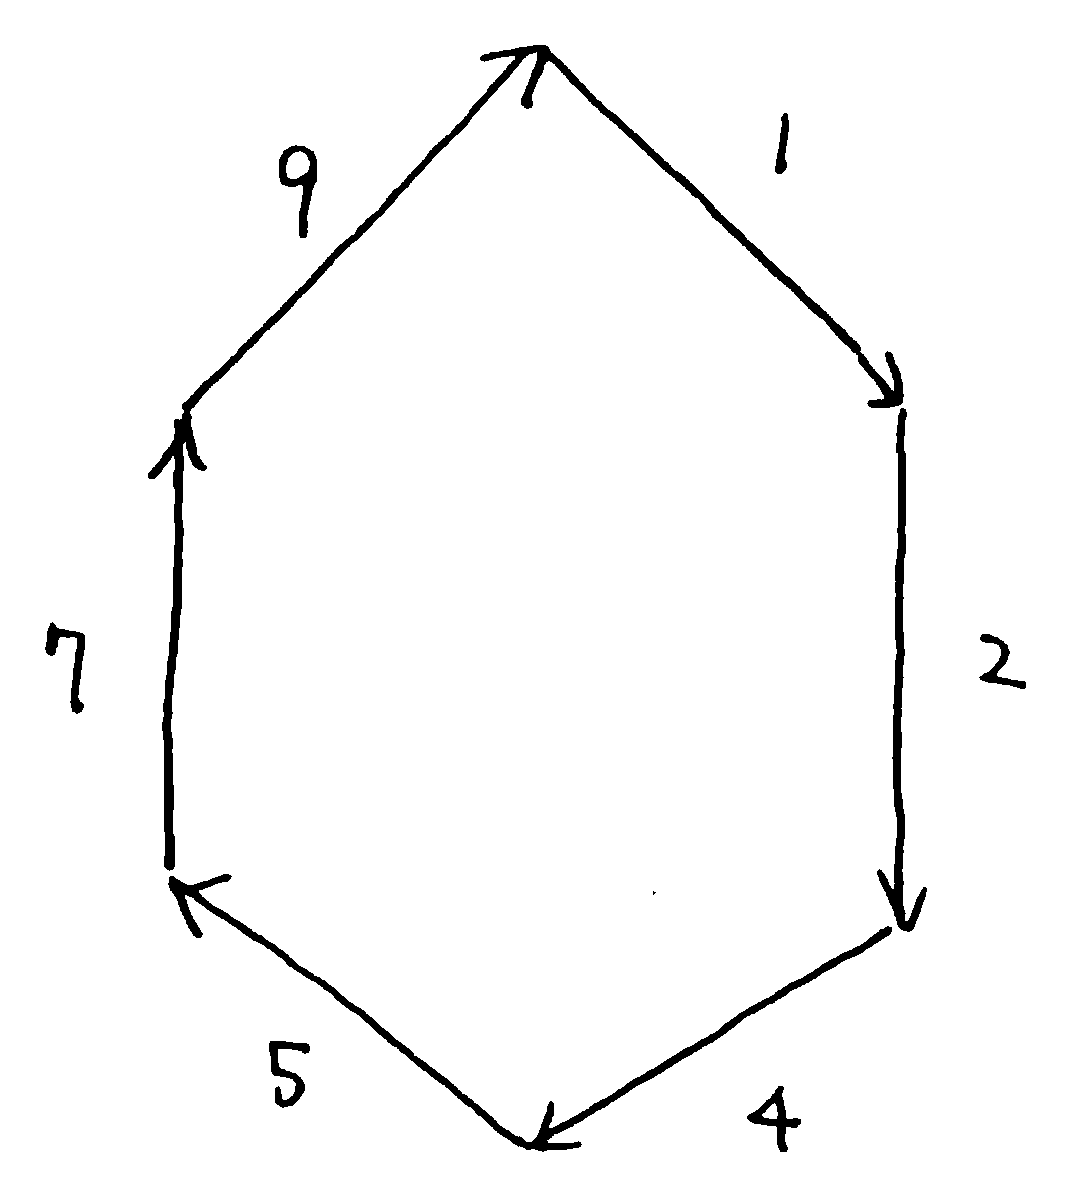
\includegraphics[width=5.0cm]{fig_p58_a.png}
\end{center}

给$\widetilde{FS}_{g,n}$的每条边赋以长度，所得的称为带度量的带标架稳定带状图，其全体记作$\widetilde{MFS}_{g,n}$。在$\widetilde{MFS}_{g,n}$中，忘掉度量信息后得到给定的$(\Gamma,G(v))\in\widetilde{FS}_{g,n}$的全体，因边界上带有标架，自然地同一视作$\R_+^a$。这里$a$是$G(v)$（$v\in V_{nc}$遍历）的边的总数。

下面定义某种等价关系。设$(\Gamma,G(v)),(\Gamma',G'(v))$为$\widetilde{S}_{g,n}$的两个元素。把$\Gamma$中以$k$条边相连的分支$v_1,v_2$替换为$v_3$，令$g(v_3)=g(v_1)+g(v_2)+(k-1)$，设由此得到$\Gamma'$。例如下图那样的替换。
\begin{center}
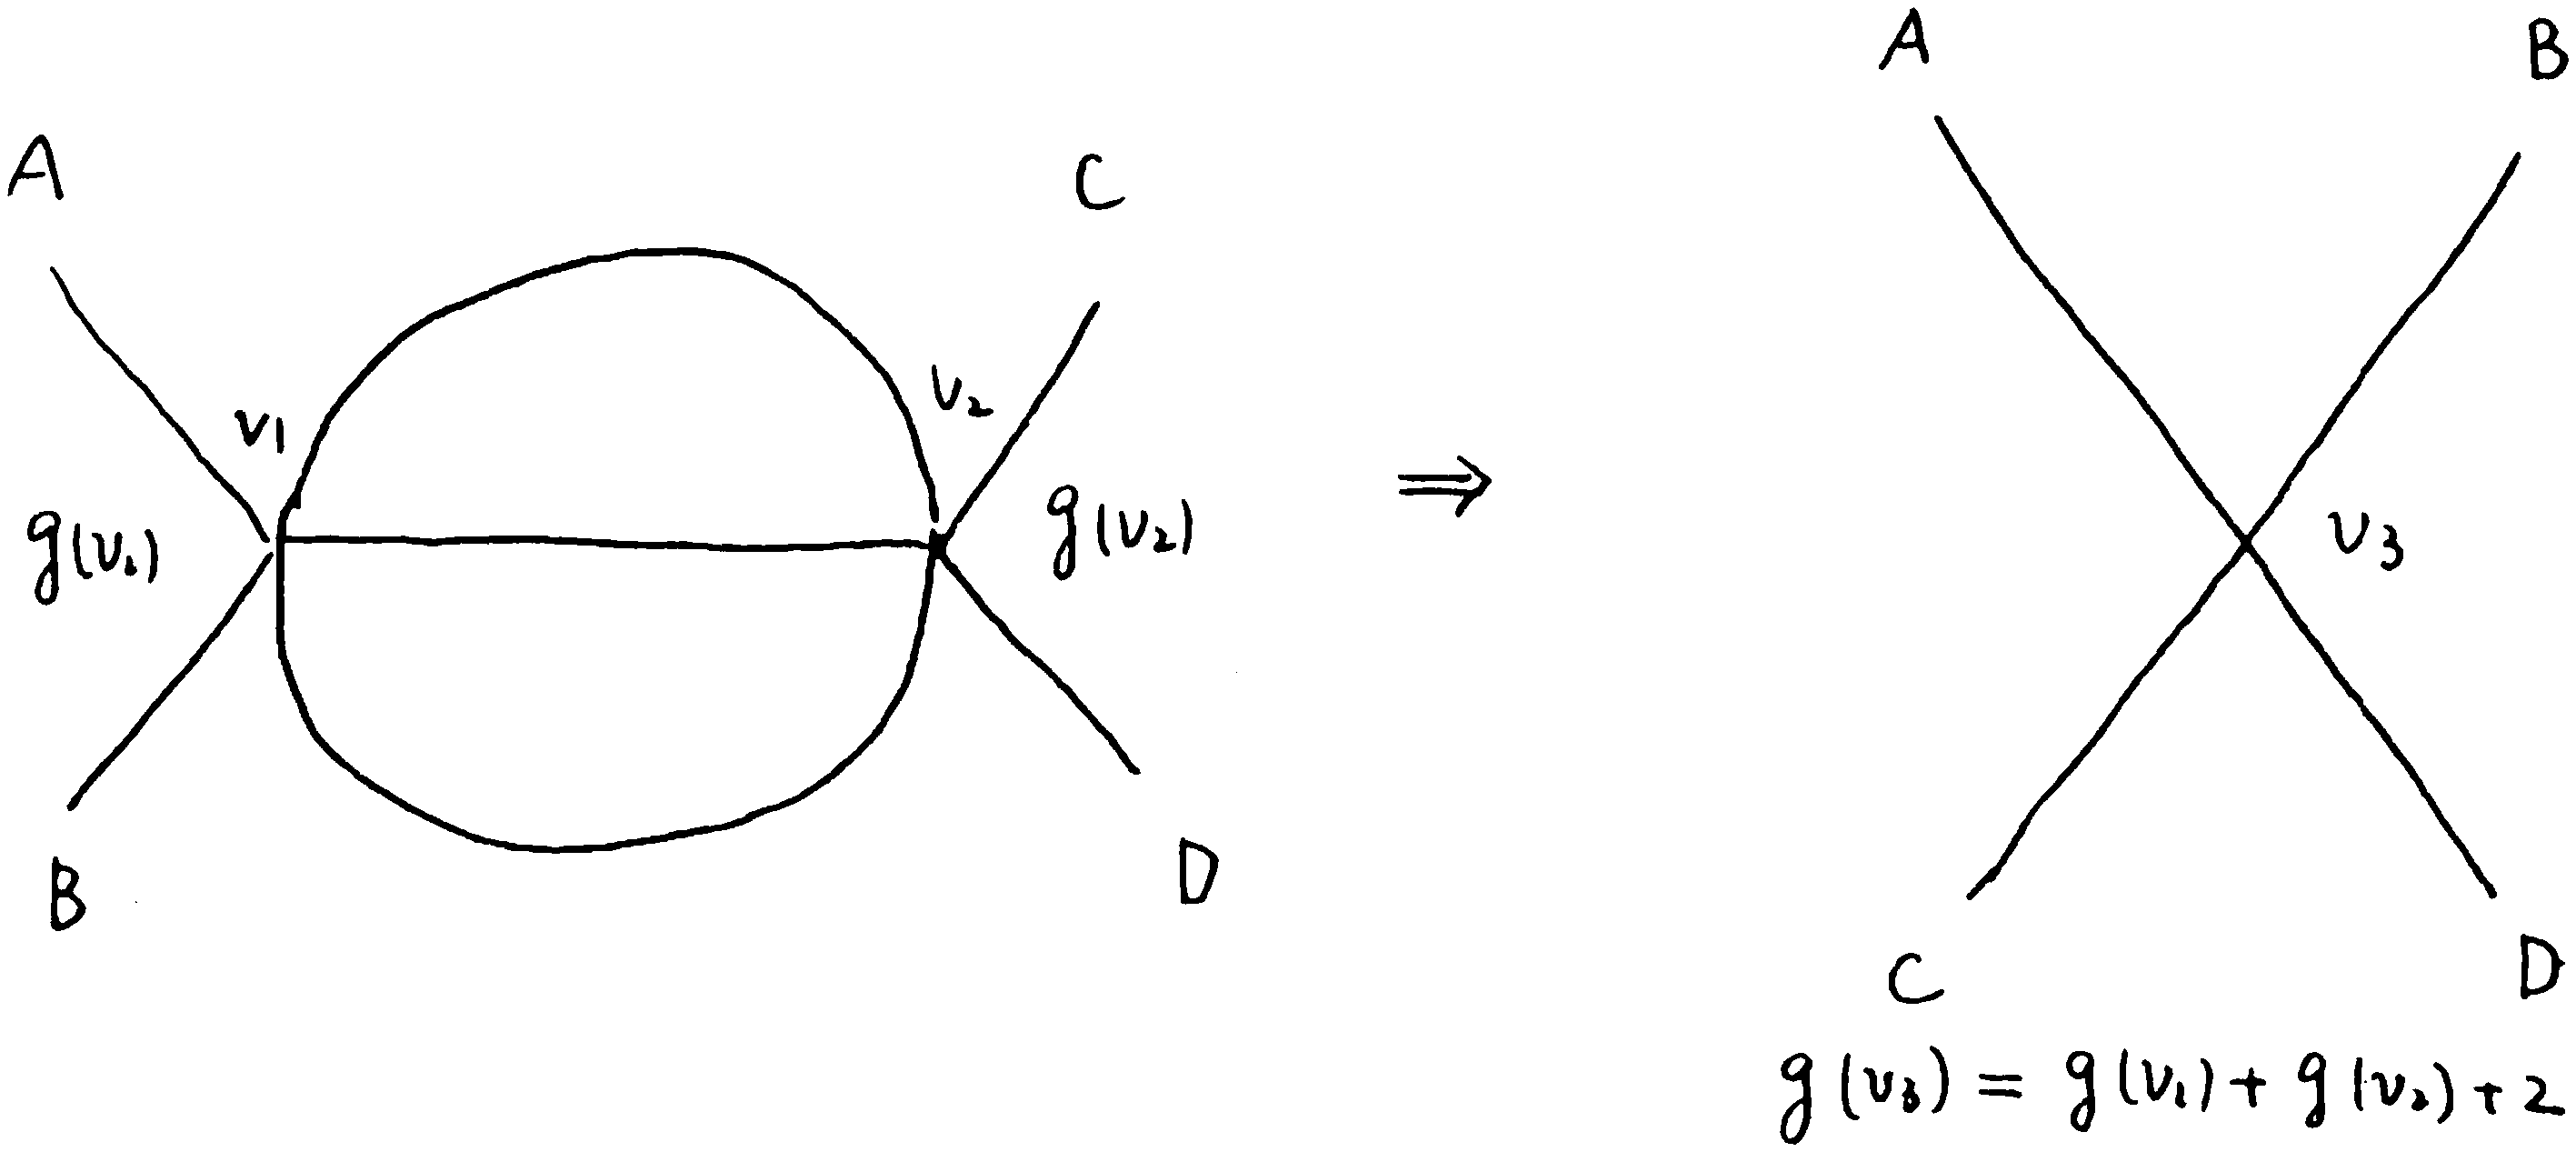
\includegraphics[width=11cm]{fig_p58_b.png}
\end{center}

此时$\Gamma,\Gamma'$的$V_{nc}$没有任何变化，故在等同视之时，设$G(v),G'(v)$作为带状图同构。

% ===== 原书 p.53 =====
考虑使这样的$(\Gamma,G(v))$与$(\Gamma',G'(v))$等价的等价关系。例如下面两个是等价的。
\begin{center}
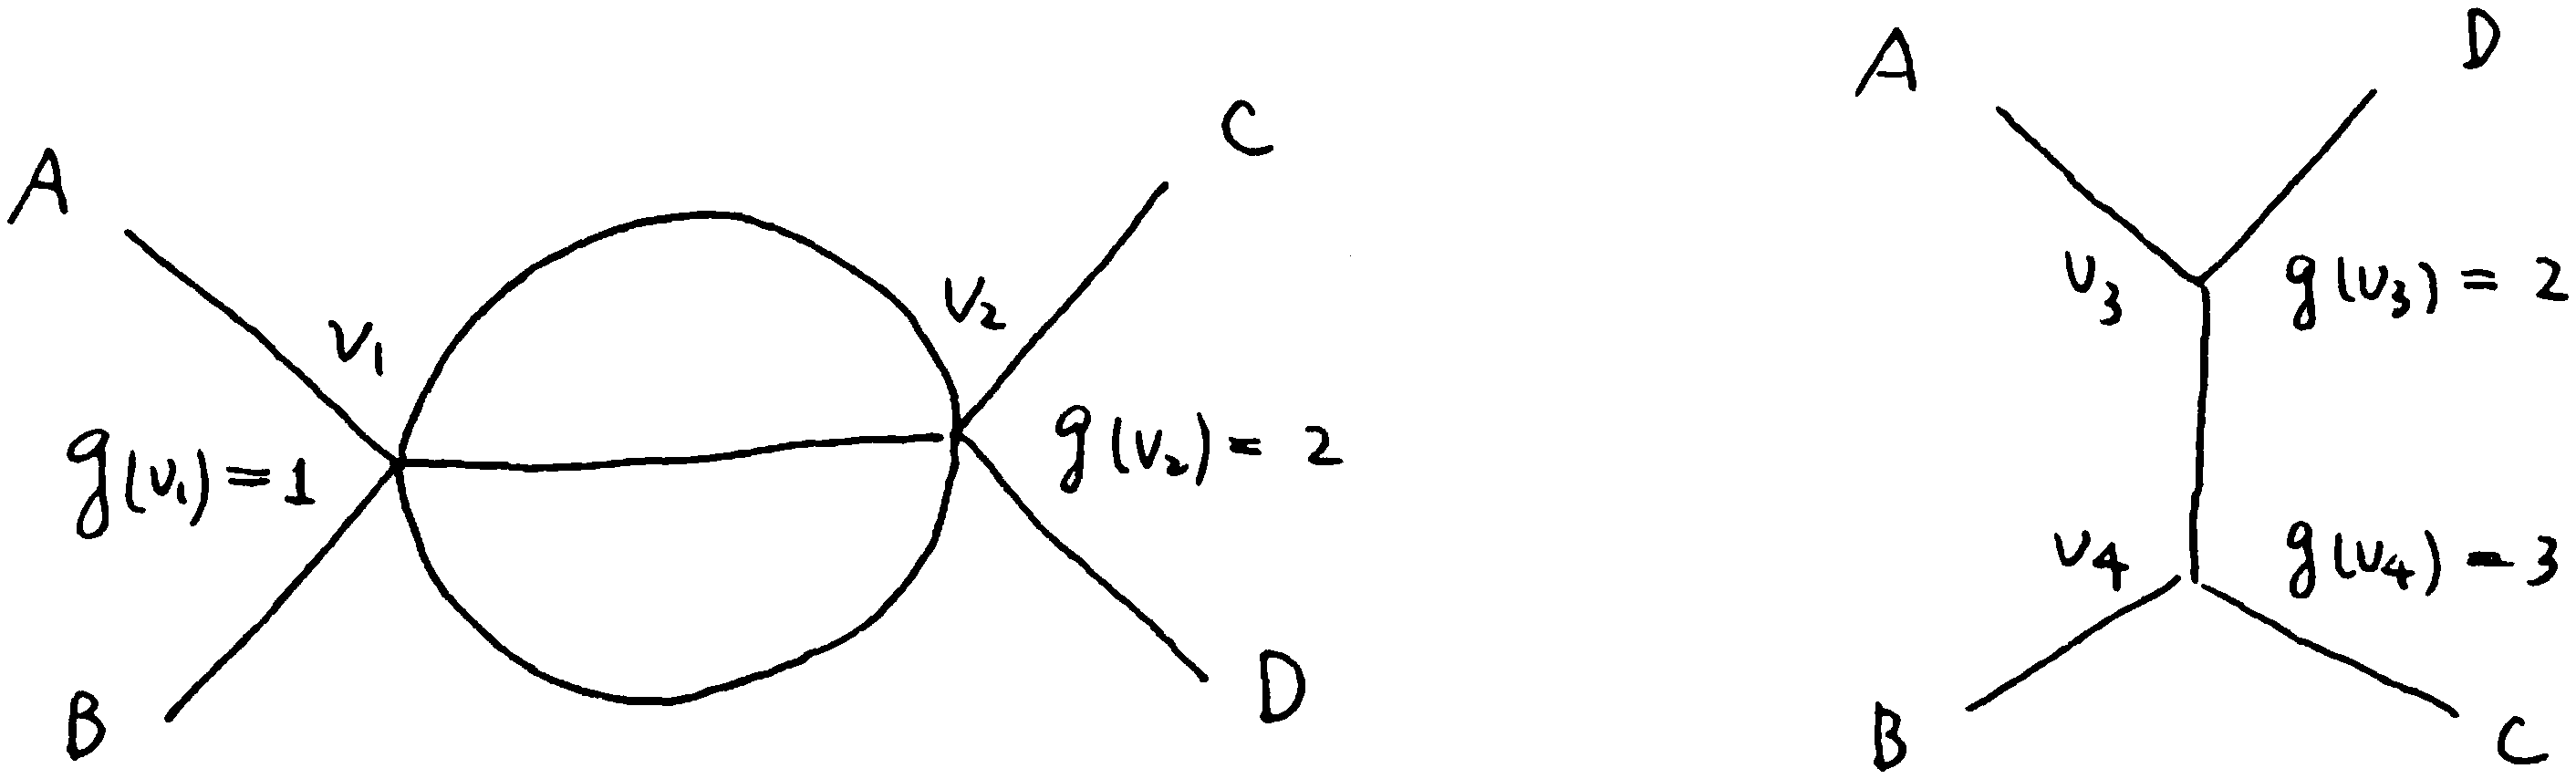
\includegraphics[width=10.5cm]{fig_p59_a.png}
\end{center}

把这个等价关系下的商空间$\widetilde{S}_{g,n}/\!\sim$定义为$S_{g,n}$。在上面的$G(v)$与$G'(v)$同构之处，按连边界的命名也算在内而同构，由此引入$\widetilde{FS}_{g,n}$上的等价关系，其商空间记作$FS_{g,n}=\widetilde{FS}_{g,n}/\!\sim$。进一步，按连度量也保持下来引入$\widetilde{MFS}_{g,n}$上的等价关系，其商空间$\widetilde{MFS}_{g,n}/\!\sim$记作$MFS_{g,n}$。此时$MFS_{g,n}$是以$(\Gamma,G(v))\in FS_{g,n}$为指标集的一族形如$\R_+^a$的空间的无交并。这里$a$如前所述，是$G(v)$（$v\in V_{nc}$）中出现的边的总数。在其上引入由度量退化而来的自然拓扑。度量退化时也会从$G(v)$生出紧分支，故为慎重起见记下其方法。例如考虑把下面的$A$与$B$粘贴所得的带状图。
\begin{center}
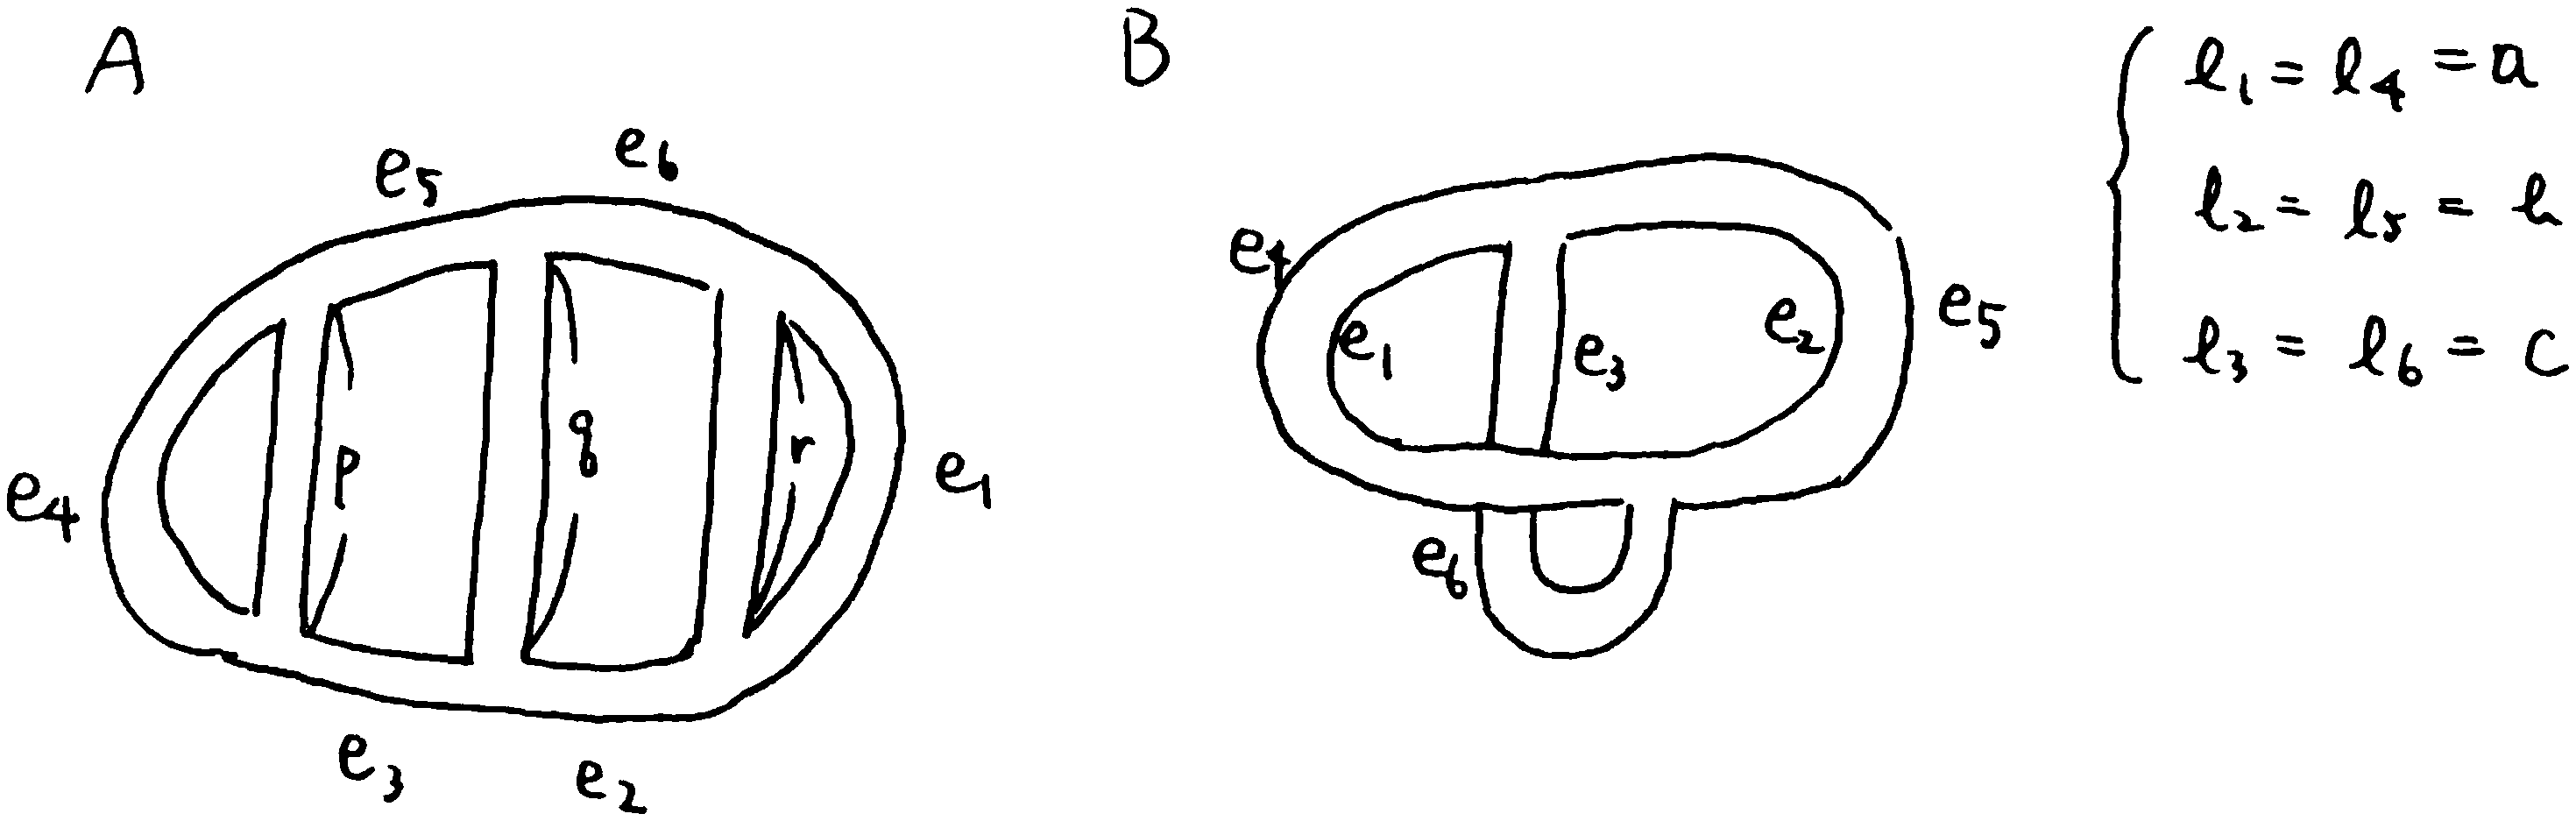
\includegraphics[width=11cm]{fig_p59_b.png}
\end{center}

这里$A$与$B$按$1\sim6$同号相粘贴，各自的长度由$a,b,c$给出。分别固定$p>0,q>0,r>0$不变而令$a+b+c\to0$时，从$B$得到亏格$1$的曲线。从$A$得到被标记$4$个点、其中$1$点为奇点的亏格$0$曲线。$A$的边界长度如图所见，收敛于$p,p+q,p+r,r$。此时亏格$0$的分支退化如下面 (c) 那样的带状图。

% ===== 原书 p.54 =====
\begin{center}
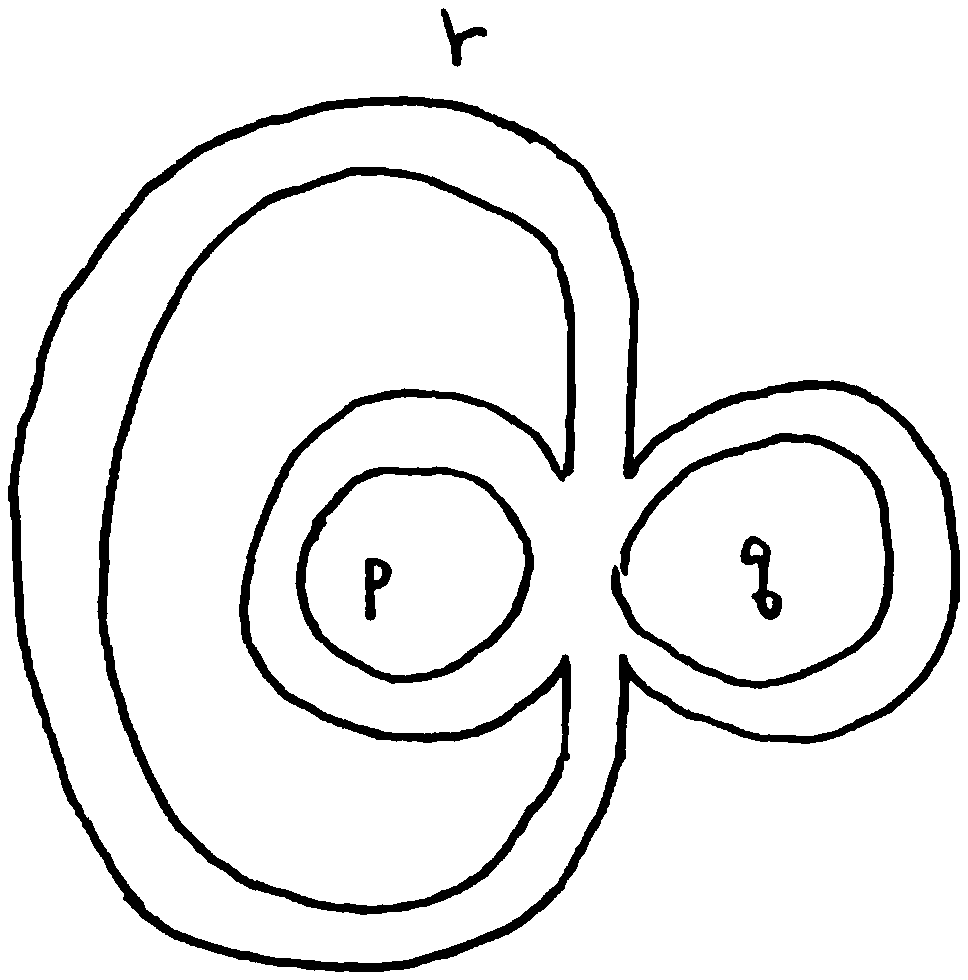
\includegraphics[width=4.5cm]{fig_p60_a.png}
\end{center}

此时，把$\R_+^6=\{(a,b,c,p,q,r)\}$与$\R_+^3=\{(0,0,0,p,q,r)\}$的并看作$\R_{\ge0}^6$，以诱导拓扑赋予拓扑。如此，$MFS_{g,n}$上就有了自然的拓扑。

又设$(\Gamma_1,G_1(v)),(\Gamma_2,G_2(v))\in MNS_{g,n}$。当忘掉$G_1(v),G_2(v)$边界上的标架后同构时，称它们作为带度量的稳定带状图同构。（这里总考虑保持边界编号的映射。）令$(\Mbar^{comb}_{g,n})_0=MFS_{g,n}$，并定义
\[
\begin{aligned}
(\Mbar^{comb}_{g,n})_1=\bigl\{&(a,b,\phi:a\rightleftarrows b)\ \bigm|\ a,b\in(\Mbar^{comb}_{g,n})_0,\\
&\phi\text{是作为带度量带状图的同构}\bigr\}.
\end{aligned}
\]

\transnote{这里写$MNS_{g,n}$，与前面定义的$MFS_{g,n}$不一致，疑为$MFS_{g,n}$之误；此处照原文译出。}

此时自然的投影$\mathrm{pr}_i$（$i=1,2$）如下定义。
\[
\begin{aligned}
(\Mbar^{comb}_{g,n})_1\ni(a,b,\phi)&\overset{\mathrm{pr}_1}{\longmapsto}a\in(\Mbar^{comb}_{g,n})_0,\\
(\Mbar^{comb}_{g,n})_1\ni(a,b,\phi)&\overset{\mathrm{pr}_2}{\longmapsto}b\in(\Mbar^{comb}_{g,n})_0.
\end{aligned}
\]

这里$\mathrm{pr}_1,\mathrm{pr}_2$遗憾地不是局部同构，但像前一章那样，令
\[
\begin{aligned}
(\Mbar^{comb}_{g,n})_k={}&(\Mbar^{comb}_{g,n})_1\times_{(\Mbar^{comb}_{g,n})_0}\cdots\\
&\times_{(\Mbar^{comb}_{g,n})_0}(\Mbar^{comb}_{g,n})_1\qquad(\text{$k$个}),
\end{aligned}
\]
构成分片线性空间的单纯对象。

\begin{definition}
\[
\Mbar^{comb}_{g,n}=\Coeq\bigl((\Mbar^{comb}_{g,n})_1\rightrightarrows(\Mbar^{comb}_{g,n})_0\bigr).
\]
又，用单纯空间$\{(\Mbar^{comb}_{g,n})_k\}_{k\ge0}$来定义$H^*(\Mbar^{comb}_{g,n},\Q)$。
\end{definition}

% ===== 原书 p.55 =====
\subsection{$BU(1)^{comb}$、$EU(1)^{comb}$与基本形式}

把空间$(BU(1)^{comb})_0$用$\varinjlim_{N}(\R_{\ge0}^N-\{0\})$定义。这里$\R_{\ge0}^N-\{0\}\to\R_{\ge0}^{N+1}-\{0\}$由$(a_1,\dots,a_N)\mapsto(a_1,\dots,a_N,0)$定义。

设$a=(a_1,\dots,a_N)\in(BU(1)^{comb})_0$。把$a_i\neq0$的$i$依次记作$a_{i_1},\dots,a_{i_m}$，考虑名为$e_{i_k}$、长度由$a_{i_k}$给出的边的环，由此对应以带度量的带基点的环。

\transnote{原文此处把满足$a_i\neq0$的下标$i$依次记作$a_{i_1},\dots,a_{i_m}$，混用了下标与分量，疑应为$i_1,\dots,i_m$；此处照原文译出。}

\begin{center}
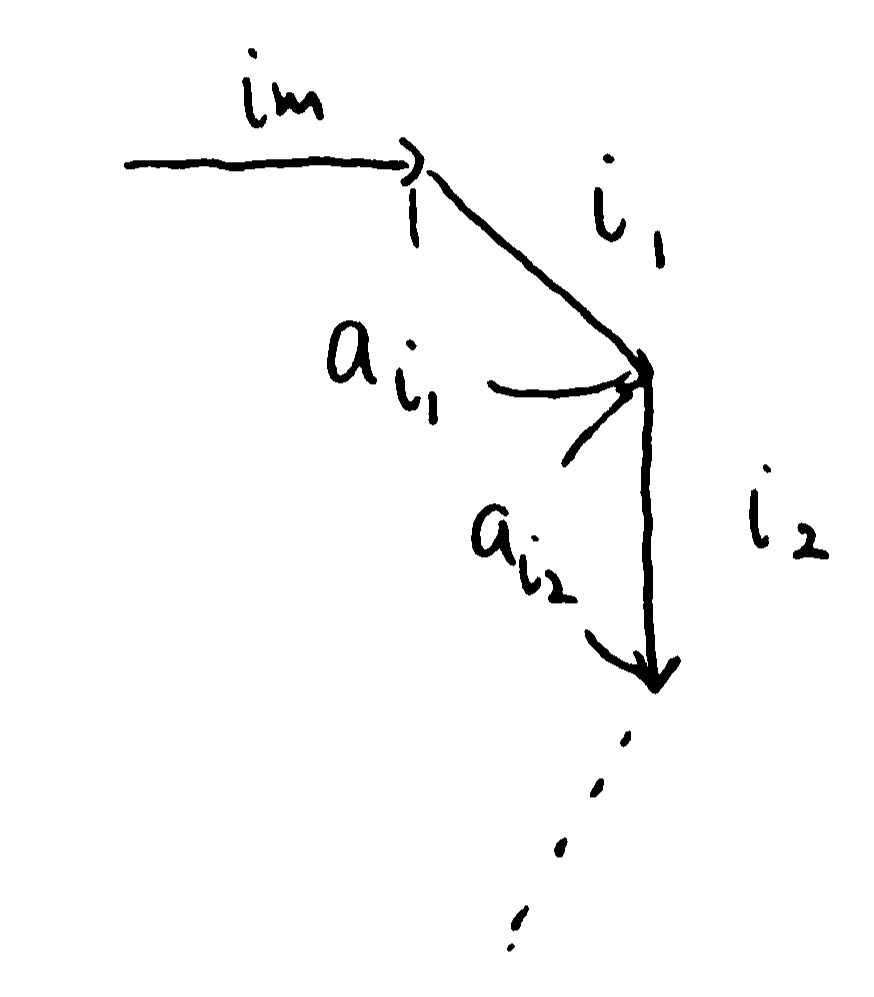
\includegraphics[width=4.0cm]{fig_p61_a.png}
\end{center}

$a,b$作为带度量的环同构，是指由$a$经重编号与重取基点得到$b$。此时把这个替换记作$\phi:a\to b$。例如取$a=(1,1,0,0)$、$b=(0,1,0,1)$，则凑巧两者长度都为$1$，故$\Hom(a,b)$是二元集合$\{\phi_1,\phi_2\}$。这里
\[
\phi_1:e_1\to e_2,\quad e_2\to e_3,\qquad
\phi_2:e_1\to e_3,\quad e_2\to e_2.
\]

\begin{center}
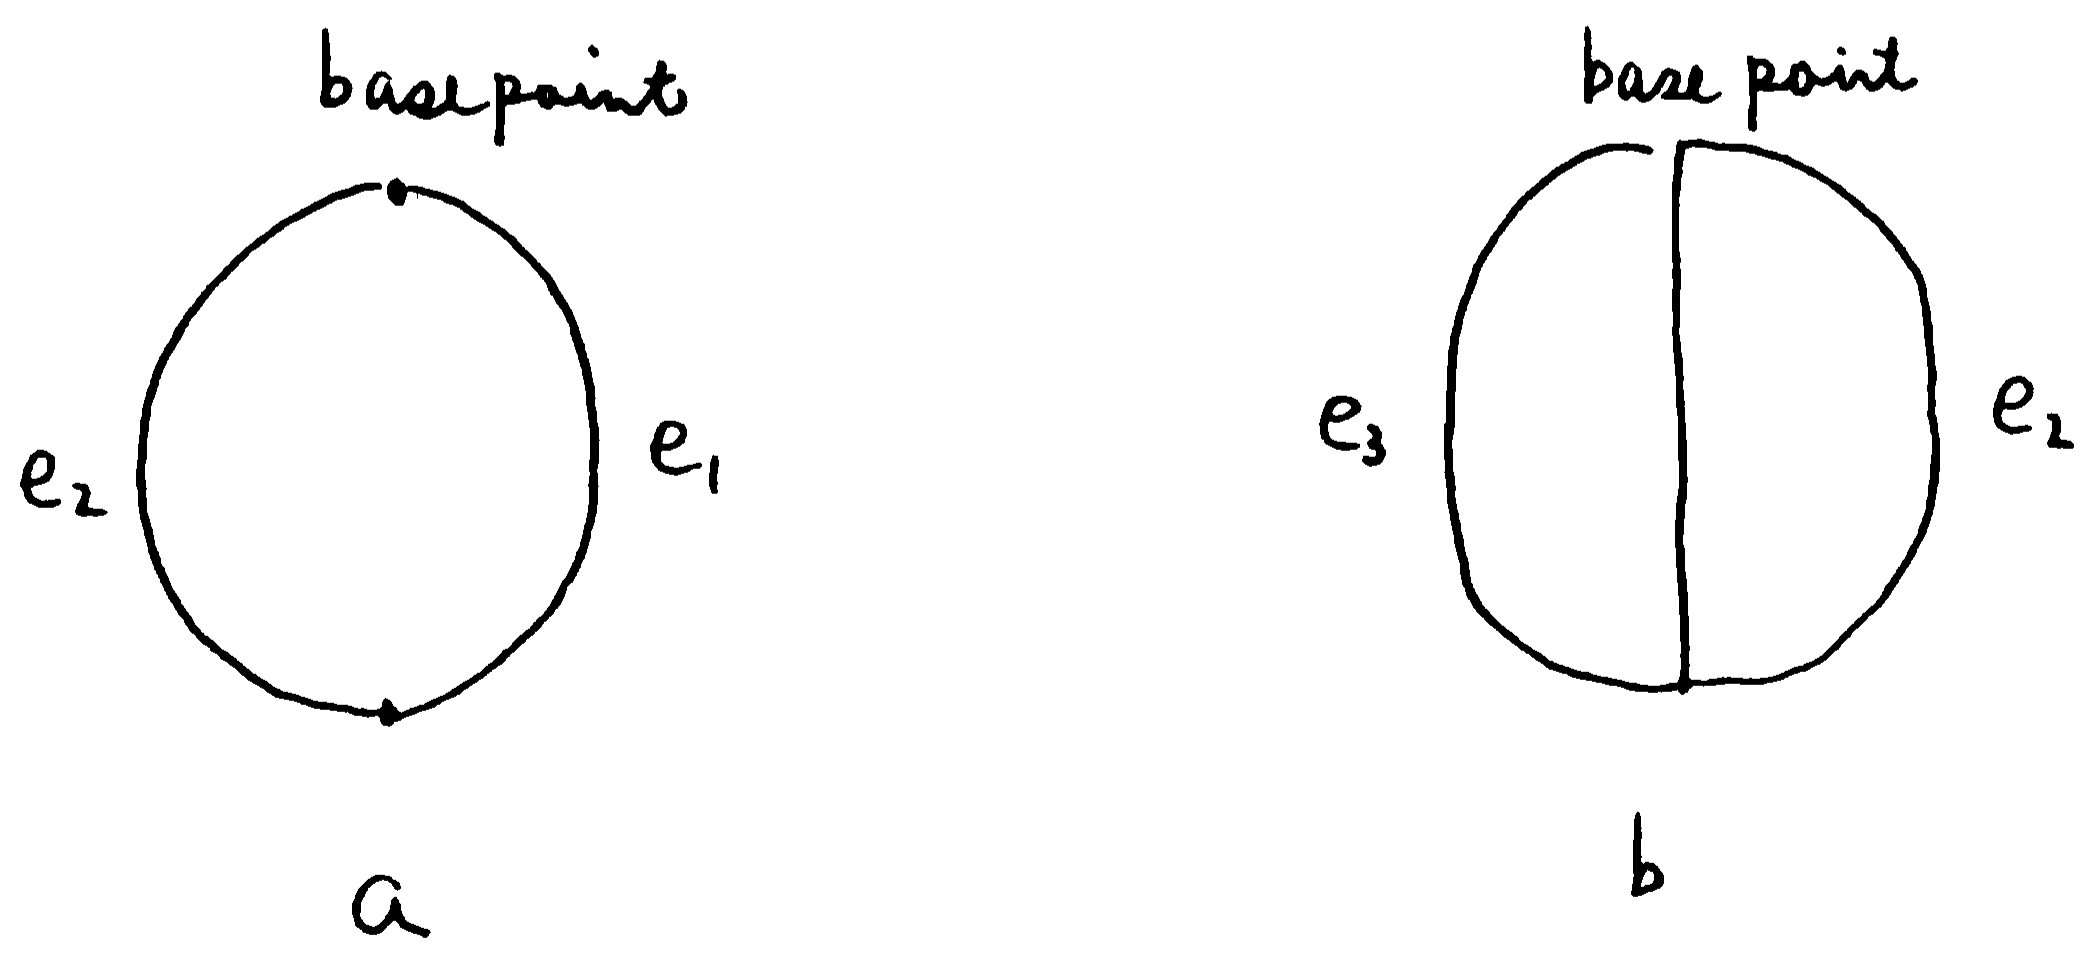
\includegraphics[width=8.5cm]{fig_p61_b.png}
\end{center}

\transnote{原文取$b=(0,1,0,1)$，其非零分量对应$e_2,e_4$，而上面的$\phi_1,\phi_2$却用到$e_3$，图 (b) 也标作$e_3,e_2$；原文前后不一致，疑$b=(0,1,1,0)$或$\phi$中应为$e_4$；此处照原文译出。}

\[
\begin{aligned}
(BU(1)^{comb})_1=\bigl\{&(a,b,\phi)\ \bigm|\ a,b\in(BU(1)^{comb})_0,\\
&\phi:a\to b\text{是作为带度量的环的同构}\bigr\}.
\end{aligned}
\]

% ===== 原书 p.56 =====
这样置定。前面所述的理由表明$\mathrm{pr}_i:(BU(1)^{comb})_1\to(BU(1)^{comb})_0$不是局部同构，但可构成分片线性单纯对象$\{(BU(1)^{comb})_k\}_k$。

\begin{definition}
\[
BU(1)^{comb}=\Coeq\bigl((BU(1)^{comb})_1\rightrightarrows(BU(1)^{comb})_0\bigr).
\]
\end{definition}

下面构成$BU(1)^{comb}$上的万有$S^1$丛$EU(1)^{comb}$。
\[
\begin{aligned}
(EU(1)^{comb})_0&=\{(a,p)\mid a\in BU(1)^{comb},\ p\in a\},\\
(EU(1)^{comb})_1&=\{(a,b,\phi,p)\mid(a,b,\phi)\in(BU(1)^{comb})_1,\ p\in a\}.
\end{aligned}
\]

此时，$(EU(1)^{comb})_1\to(EU(1)^{comb})_0\times(EU(1)^{comb})_0$是单射，其像给出$(EU(1)^{comb})$上的等价关系。把这个等价关系下的商空间$(EU(1)^{comb})_0/\!\sim$中对应多边形$a$的边数恰好为$N$的部分记作$EU(1)^{comb}_N$，则它与下面的空间同一视。
\[
\begin{aligned}
\bigl\{(r,\phi_1,\dots,\phi_N)\ \bigm|\ &r\in\R_+,\ \phi_i\in\R/r\Z,\ \phi_i\neq\phi_{i+1},\\
&\phi_i\text{沿环排列},\ \phi_N\le0<\phi_1\bigr\}.
\end{aligned}
\]

在这个空间上取局部坐标$(r,\tilde\phi_1,\dots,\tilde\phi_N)$。这里$\tilde\phi_i\in\R$是$\phi_i$在$\R$中的代表元。此时$d(\tilde\phi_i/r)$不依赖坐标的取法，故记作$d(\phi_i/r)$。取满足$l_i\equiv\phi_{i+1}-\phi_i\bmod r\Z$、$0\le l_i<r$的函数$l_i$，用它定义$EU(1)^{comb}_N$上的$1$次形式
\[
\alpha=\sum_{i=1}^{N}\frac{l_N}{r}\wedge d\Bigl(\frac{\phi_i}{r}\Bigr).
\]

\transnote{上式第$i$项的系数原文印作$l_N/r$，与随后对$d\alpha$的计算及各系数$l_1,\dots,l_N$不符，疑应为$l_i/r$；此处照原文译出。}

现固定$l_1,\dots,l_N>0$，置
\[
\begin{aligned}
S^1(l_1,\dots,l_N)=\bigl\{(r,\phi_1,\dots,\phi_N)\in EU(1)^{comb}_N\ \bigm|\ &r=l_1+\cdots+l_N,\\
&l_i\equiv\phi_{i+1}-\phi_i\ (\mathrm{mod}\ r\Z)\bigr\}.
\end{aligned}
\]

% ===== 原书 p.57 =====
则$\int_{S^1(l_1,\dots,l_N)}\alpha=-1$。按下图作坐标变换$(r,\phi_1,\dots,\phi_N)\mapsto(l_1,\dots,l_N,t)$（$0\le t<l_N$）：
\[
\phi_1=l_N-t,\qquad \phi_2=l_1+l_N-t,\ \dots
\]
\begin{center}
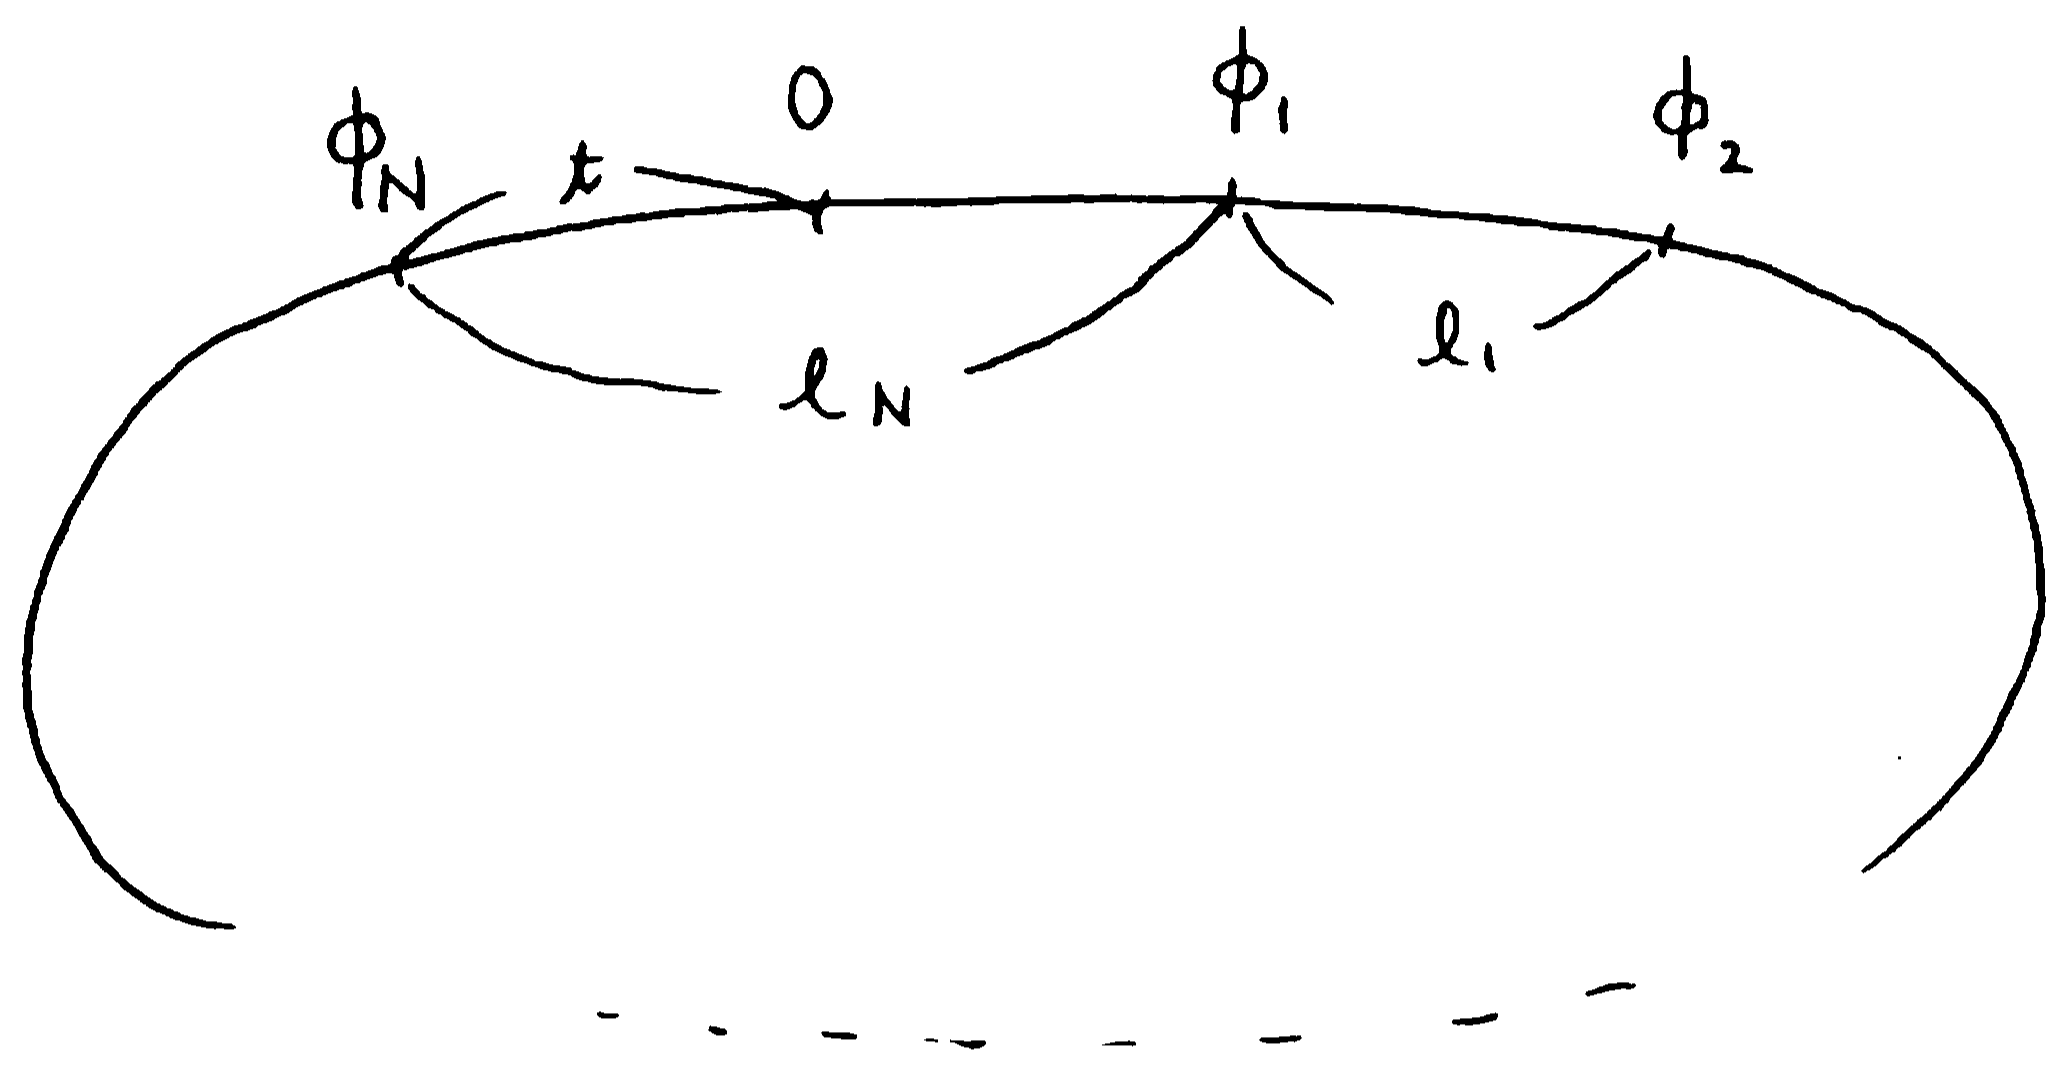
\includegraphics[width=8.0cm]{fig_p63_a.png}
\end{center}

此时，$\alpha$表示为
\[
\begin{aligned}
\alpha&=\frac{l_1}{r}\wedge d\Bigl(\frac{l_N-t}{r}\Bigr)
+\frac{l_2}{r}\wedge d\Bigl(\frac{l_1+l_N-t}{r}\Bigr)\\
&\qquad+\cdots+\frac{l_N}{r}\wedge d\Bigl(\frac{l_{N-1}+\cdots+l_1+l_N-t}{r}\Bigr),
\end{aligned}
\]
并且$d\alpha$作为$EU(1)^{comb}_N$上的$2$次形式表示为
\[
\begin{aligned}
\omega=d\alpha
&=d\Bigl(\frac{l_1}{r}\Bigr)\wedge d\Bigl(\frac{l_N}{r}\Bigr)
+d\Bigl(\frac{l_2}{r}\Bigr)\wedge d\Bigl(\frac{l_1+l_N}{r}\Bigr)+\cdots\\
&\quad-\Bigl(d\Bigl(\frac{l_1}{r}\Bigr)\wedge d\Bigl(\frac{t}{r}\Bigr)
+d\Bigl(\frac{l_2}{r}\Bigr)\wedge d\Bigl(\frac{t}{r}\Bigr)
+\cdots+d\Bigl(\frac{l_N}{r}\Bigr)\wedge d\Bigl(\frac{t}{r}\Bigr)\Bigr)\\
&=\sum_{1\le j\le i\le N-1}d\Bigl(\frac{l_i}{r}\Bigr)\wedge d\Bigl(\frac{l_j}{r}\Bigr),
\end{aligned}
\]
不再依赖坐标$t$。

下面想说明$\omega$给出$BU(1)^{comb}$中对应于$N$边形的子单纯空间$BU(1)^{comb}_N$上的微分形式$\omega$。为此必须说明$\omega$在变换$(l_1,\dots,l_N)\mapsto(l_2,\dots,l_N,l_1)$下不变。这可用$d(l_N/r)+\cdots+d(l_N/r)=0$来证明。又，限制到某个$l_i=0$的子单纯空间时，它与$BU(1)^{comb}_{N-1}$上的$\omega$形状相同。由此，$\omega$决定了$BU(1)^{comb}$上的$2$次形式。又由$\omega$的构成方法可知$d\omega=0$，故它决定了$H^2_{DR}(BU(1)^{comb})$的元素$u_1$。

\transnote{上式$d(l_N/r)+\cdots+d(l_N/r)=0$的末项疑应为$d(l_1/r)$；此处照原文译出。}

% ===== 原书 p.58 =====
% （本页开头是上页末句的结尾，本块已把它并入上一段译完；以下从略。
%   本页余下的$\partial_i$与§3.4 开头属 c08。）
称$\omega$为$BU(1)^{comb}$的万有基本形式，$u_1$为$BU(1)^{comb}$的万有基本类。

% =====================================================================
%  c08 —— PDF p.64–69（原书 p.58–63）
%  §3.4 M̄_{g,n} 的相交理论
% =====================================================================

% ===== 原书 p.58 =====
% （本页开头一句「称 ω 为 BU(1)^{comb} 的万有基本形式，u_1 为……万有基本类。」
%   已由 c07 译完，本块自此段起译。）
现在，对$i=1,\dots,n$，设
\[
\partial_i:\Mbar^{comb}_{g,n}\longrightarrow BU(1)^{comb}
\]
为把各边界的带编号图与之对应的映射。此时$\partial_i$诱导出上同调之间的映射
\[
\partial_i^*:H^*_{DR}(BU(1)^{comb})\longrightarrow H^*_{DR}(\Mbar^{comb}_{g,n}),
\]
并把$u_1$在$\partial_i^*$下的像记作$c_i$（$i=1,\dots,n$）。又由 de Rham 定理，把与$u_i$对应的$H^i(\MbarGN)$的元素记作$c_{i,sing}$。

\transnote{原文此句写「与$u_i$对应的$H^i(\MbarGN)$的元素」，但前文只定义了$u_1$（即$H^2_{DR}(BU(1)^{comb})$的元素），$H$的次数也应为$2$；此处照原文译出。}

\subsection{$\MbarGN$的相交理论}

由 Deligne–Mumford 的可表示性，$\MbarGN$在代数意义下具有平展且可表示的覆盖$X_0$。把其伴随解析空间记作$X_0^{an}$。现在，对于$x=(C,p_1,\dots,p_n,r_1,\dots,r_n)\in X_0^{an}\times\R_+^n$，考虑$C_v$（$v\in V_{nc}$）上具有闭轨道且满足下述条件的二次微分$\omega$：
\begin{enumerate}[label=(\arabic*)]
\item 若$p_i\in C_v$，则关于由$\omega_v$确定的度量，$p_i$周围的闭轨道的长度为$r_i$。
\item 特征环域仅为$p_i$周围的小闭曲线。
\item 对属于$C_v$的$C$的奇点，$\omega_v$具有至多$1$阶极点。
\end{enumerate}
由此得到的带度量的稳定带状图记作$(\Gamma_x,G_x(v))$。此时，设$X_0^{an}\times\R_+^n$有足够细的覆盖$X_0^{an}\times\R_+^n=\cup U_k$，且满足下述条件。在各$U_k$上，$\{G_x(v)\}_v$的第$i$个边界上定有连续的标架。不过这里所说的连续标架，也允许退化的情形。

% ===== 原书 p.59 =====
即，也允许下面那样的标架。

\begin{center}
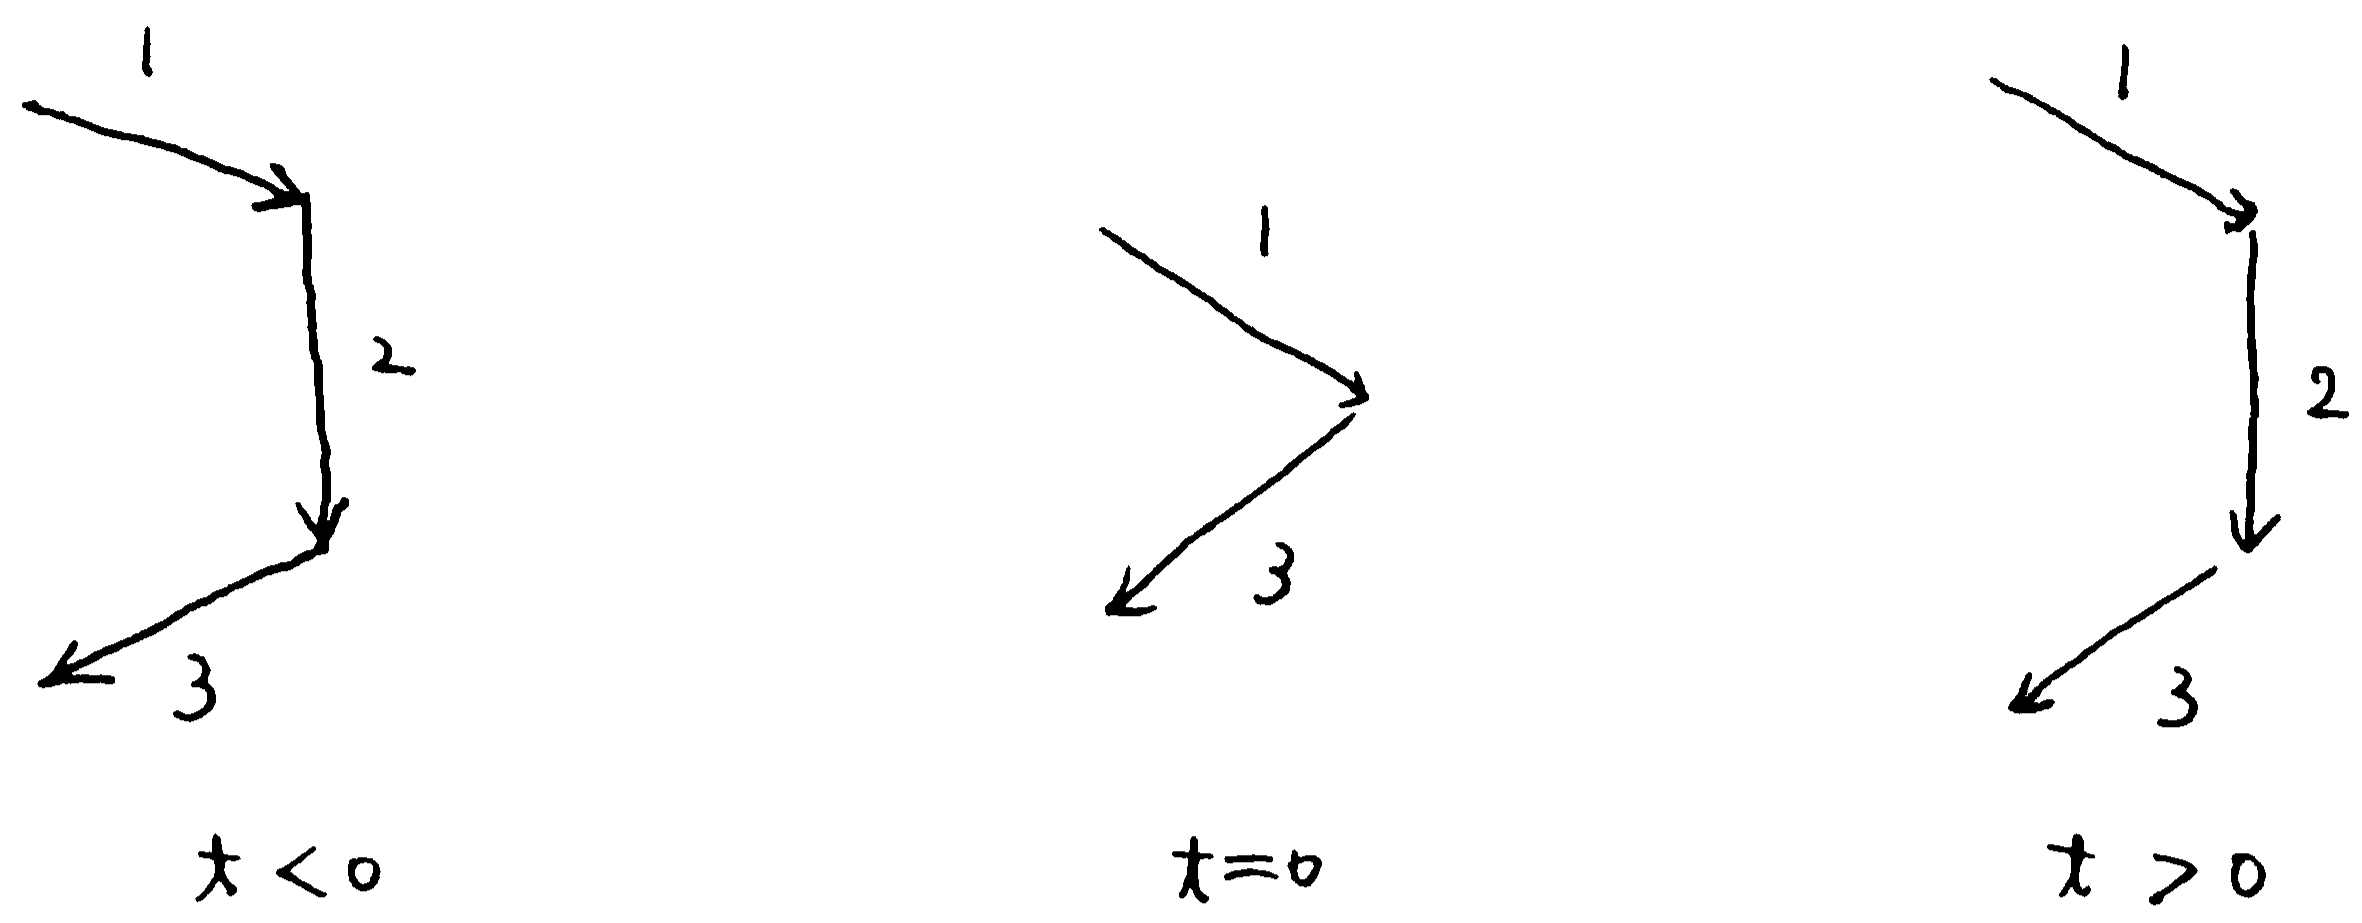
\includegraphics[width=0.62\linewidth]{fig_p65_a.png}
\end{center}

对各个$U_i$固定一个边界的标架，由此定义连续映射
\[
\coprod U_i\longrightarrow(\Mbar^{comb}_{g,n})_0.
\]
重新置$Y_0=\coprod U_i$，并置$Y_1=Y_0\times_{(\MbarGN\times\R_+^n)^{an}}Y_0$，则$Y_1$到$(\Mbar^{comb}_{g,n})_1$自然诱导出连续映射，故作为余等化子的映射
\[
f:\Mbar^{an}_{g,n}\times\R_+^n\longrightarrow\Mbar^{comb}_{g,n}
\]
被定义。由此，经由到单纯空间的诱导映射，可定义奇异同调、奇异上同调的映射
\[
\begin{aligned}
H_*(\MbarGN\times\R_+^n,\Q)&\xrightarrow{f_*}H_*(\Mbar^{comb}_{g,n},\Q),\\
H^*(\Mbar^{comb}_{g,n},\Q)&\xrightarrow{f^*}H^*(\MbarGN\times\R_+^n,\Q).
\end{aligned}
\]
在 de Rham 上同调中，类似的映射也被预期可以诱导出来，但因稍难理解，此处不作讨论。现在，把$\MbarGN$上的线丛$s_i^*(T_{\mathcal{C}/\MbarGN})$记作$\mathcal{L}_i$。这里$\mathcal{C}\to\MbarGN$为万有曲线。此时，$\mathcal{L}_i$的 Chern 类$c_1(\mathcal{L}_i)$定在$H^2(\MbarGN,\R)$中。进一步此时，

\begin{proposition}
\[
f^*(c_{i,sing})=pr_1^*\bigl(c_1(\mathcal{L}_i)\bigr).
\]
\end{proposition}

这里$\mathrm{pr}_1^*$是自然诱导映射
\[
\mathrm{pr}_1^*:H^*(\MbarGN,\R)\longrightarrow H^*(\MbarGN\times\R_+^n,\R).
\]

% ===== 原书 p.60 =====
现在固定$\mathbf{r}=(r_1,\dots,r_r)\in\R_+^n$，考虑包含映射
\[
i_{\mathbf{r}}:\MbarGN\hookrightarrow\MbarGN\times\R_+^n;\quad x\mapsto(x,\mathbf{r}).
\]
则$\mathrm{pr}_1\circ i_{\mathbf{r}}=\id$。因$\dim\MbarGN=6g-6+2n$，故当$d_1+\cdots+d_n=3g-3+n$时，有$c_1(\mathcal{L}_1)^{d_1}\wedge\cdots\wedge c_1(\mathcal{L}_n)^{d_n}\in H^{6g-6+2n}(\MbarGN,\Q)$，从而
\[
\tr_{\MbarGN}\bigl(c_1(\mathcal{L}_1)^{d_1}\wedge\cdots\wedge c_1(\mathcal{L}_n)^{d_n}\bigr)\in\Q .
\]

\transnote{原文此处写$\mathbf{r}=(r_1,\dots,r_r)\in\R_+^n$，最后一个下标与前面的$r_1$不一致，疑应为$r_n$；此处照原文译出。}

迹映射$H^{6g-6+2n}(\MbarGN,\Q)\to\Q$与$H_{6g-6+2n}(\MbarGN,\Q)\ni[\MbarGN]$的自然配对一致，故
\[
\begin{aligned}
&\tr_{\MbarGN}\bigl(c_1(\mathcal{L}_1)^{d_1}\wedge\cdots\wedge c_1(\mathcal{L}_n)^{d_n}\bigr)\\
&\quad=\bigl([\MbarGN],c_1(\mathcal{L}_1)^{d_1}\wedge\cdots\wedge c_1(\mathcal{L}_n)^{d_n}\bigr)\\
&\quad=\bigl([\MbarGN],i_{\mathbf{r}}^*pr_1^*\bigl(c_1(\mathcal{L}_1)^{d_1}\wedge\cdots\wedge c_1(\mathcal{L}_n)^{d_n}\bigr)\bigr)\\
&\quad=\bigl(i_{\mathbf{r},*}[\MbarGN],(pr_1^*c_1(\mathcal{L}_1))^{d_1}\wedge\cdots\wedge(pr_1^*c_1(\mathcal{L}_n))^{d_n}\bigr)\\
&\quad=\bigl(i_{\mathbf{r}*}[\MbarGN],(f^*c_1)^{d_1}\wedge\cdots\wedge(f^*c_n)^{d_n}\bigr)\\
&\quad=\bigl(f_*i_{\mathbf{r},*}[\MbarGN],c_1^{d_1}\wedge\cdots\wedge c_n^{d_n}\bigr)
\end{aligned}
\]
成立。现在置$f_*i_{\mathbf{r},*}[\MbarGN]=[\Mbar^{comb}_{g,n}]$，构造代表$[\Mbar^{comb}_{g,n}]$的闭链$\Mbar^{comb}_{g,n}$。若能办到，则由$\Mbar^{comb}_{g,n}$处的 de Rham 定理，
\[
\bigl(f_*i_{\mathbf{r},*}[\MbarGN],c_1^{d_1}\wedge\cdots\wedge c_n^{d_n}\bigr)
=\int_{\Mbar^{comb}_{g,n}}c_1^{d_1}\wedge\cdots\wedge c_n^{d_n}
\]
成立。现在，设$TG_{g,n}$为亏格$g$、边界个数为$n$的三价带状图（但边界已编号）的集合。对$TG_{g,n}$的每个元素$G$，各边界上的标架各取一个，以下固定此标架。对$G$，令$\Delta_{G,\mathbf{r}}$为使$G$的度量中$p_i$处的边界长度为$r_i$的度量的全体。利用$G$为三价这一点，其边数为$6g-6+3n$。故$\Delta_{G,\mathbf{r}}$是$\R_+^{6g-6+3n}$内的$(6g-6+2n)$维多面体。对此，亏格$g$的

% ===== 原书 p.61 =====
$n$点 Riemann 面的族$C_{G,\mathbf{r}}$在$\Delta_{G,\mathbf{r}}$上构成，由此定出$\Delta_{G,\mathbf{r}}$到$\MbarGN$的映射。现在，设$U\to T$为$Aut(G)$-主丛，且给定等变映射$U\to\Delta_{G,\mathbf{r}}$，则把$\Delta_{G,\mathbf{r}}$上的 Riemann 面的族$C_{G,\mathbf{r}}$拉回到$U$上，其上便诱导出$G$的作用。由于此作用自由，可得$T$上的 Riemann 面的族。即，
\[
\bigl[\Delta_{G,\mathbf{r}}/Aut(G)\bigr]\longrightarrow\MbarGN
\]
的映射被定义。且此映射成为单射。由此可知，$\sum_{G\in TG_{g,n}}\frac{1}{Aut(G)}\Delta_{g,n}$是$[\MbarGN]\in H_{6g-6+2n}(\MbarGN)$的代表。又可知，它自然给出$\Mbar^{comb}_{g,n}$的$(6g-6+2n)$维闭链。把它置作$\Mbar^{comb}_{g,n,\mathbf{r}}$，则由$i_{\mathbf{r}}$的定义得$f_*i_{\mathbf{r},*}[\MbarGN]=[\Mbar^{comb}_{g,n,\mathbf{r}}]$。

(1)
\[
\Mbar^{comb}_{g,n,\mathbf{r}}=\sum_{G\in TG_{g,n}}\frac{1}{Aut(G)}\Delta_{G,\mathbf{r}}
\]

把(1)、(2)合起来，得到下面的定理。

\transnote{原文此处引用 (2)，但本页及前页只给 (1) 编了号，上一页中迹与相交数相等的等式链并未编号；此处照原文译出。}

\begin{theorem}
\[
\langle\tau_{d_1},\dots,\tau_{d_n}\rangle
=\sum_{G\in TG_{g,n}}\frac{1}{Aut(G)}\int_{\Delta_{G,\mathbf{r}}}c_1^{d_1}\wedge\cdots\wedge c_n^{d_n}
\]
\end{theorem}

这里
\[
c_i=\sum_{1\le j\le k\le N_i-1}d\Bigl(\frac{l_k}{r_i}\Bigr)\wedge d\Bigl(\frac{l_j}{r_i}\Bigr),
\]
$N_i$为边界$\partial_i$的个数，$l_1,\dots,l_{N_i}$为按$G$的标架的顺序排列的、出现在$\partial_i$中的边的长度。

由此，相交数完全用组合的数表出。此处，在开始计算右端之前，先对$\mathbf{r}$作 Radon 变换。设$f(\mathbf{r})=f(r_1,\dots,r_n)$为$\R_+^n$上可积的函数。由上述定理 3.5 与 Fubini 定理，
\[
\begin{aligned}
&\Bigl(\int_{\R_+^n}f(\mathbf{r})dr_1\wedge\cdots\wedge dr_n\Bigr)
\langle\tau_{d_1},\dots,\tau_{d_n}\rangle\\
&\quad=\sum_{G\in TG_{g,n}}\frac{1}{Aut(G)}
\int_{\Delta_G}f(\mathbf{r})c_1^{d_1}\wedge\cdots\wedge c_n^{d_n}\wedge dr_1\wedge\cdots\wedge dr_n
\end{aligned}
\]

% ===== 原书 p.62 =====
成立。这里$\Delta_G$为$G$的全部度量的全体，经$G$的边界的标架与$\R_+^{6g-6+2n}$等同。现在，取$\lambda_1,\dots,\lambda_n\in\R$，对
\[
f(\mathbf{r})=\prod_i\frac{1}{d_i!}\exp(-\lambda_1r_1-\cdots-\lambda_nr_n)r_1^{2d_1}\cdots r_n^{2d_n}
\]
应用上式，再对满足$d_1+\cdots+d_n=3g-3+n$、$d_1\ge0,\dots,d_n\ge0$的$d_1,\dots,d_n$求和，便得下述等式。

\begin{proposition}
\[
\begin{aligned}
&\sum_{d_1+\cdots+d_n=3g-3+n}\prod_i\frac{1}{d_i!}\langle\tau_{d_1},\dots,\tau_{d_n}\rangle\\
&\qquad\times\int\exp(-\lambda_1r_1-\cdots-\lambda_nr_n)r_1^{2d_1}\cdots r_n^{2d_n}dr_1\wedge\cdots\wedge dr_n\\
&=\sum_{G\in TG_{g,n}}\frac{1}{d!Aut(G)}\int_{\Delta_G}\exp(-\lambda_1r_1-\cdots-\lambda_nr_n)\\
&\qquad\times(r_1^2c_1+\cdots+r_n^2c_n)^d dr_1\wedge\cdots\wedge dr_n
\end{aligned}
\]
\end{proposition}

其次，把两边看作关于$\lambda_1,\dots,\lambda_n$的函数等式。先看左边，利用等式
\[
\int_0^\infty\exp(-\lambda r)r^{2d}dr=\frac{(2d)!}{\lambda^{2d+1}}
\]
可得
\[
\sum_{d_1+\cdots+d_n=3g-3+n}\langle\tau_{d_1},\dots,\tau_{d_n}\rangle
\prod_{i=1}^n\frac{(2d_i-1)!!}{\lambda_i^{2d_i+1}}.
\]
计算右边需要下面的引理。

\begin{lemma}[Kontsevich {[K]}，定理 C.1]
置$\Omega=\sum_{i=1}^nr_i^2c_i$，则
\[
\frac{\Omega^d}{d!}dr_1\wedge\cdots\wedge dr_n=2^{5g-5+2n}\prod_{e\in G^{(1)}}dl_e
\]
成立。这里$G^{(1)}$为$G$的边的集合。
\end{lemma}

证明从略。利用上述引理 3.7，命题 3.6 的右端可表为
\[
\begin{aligned}
&\sum_{G\in TG_{g,n}}\frac{2^{5g-5+2n}}{Aut(G)}
\int_{\Delta_G}\exp(-\lambda_1r_1-\cdots-\lambda_nr_n)\prod_{e\in G^{(1)}}dl_e\\
&=\sum_{G\in TG_{g,n}}\frac{2^{-4g+4-2n}}{Aut(G)}\prod_{e\in G^{(1)}}\frac{2}{\tilde\lambda(e)}.
\end{aligned}
\]
这里，当$e\in G^{(1)}$为边界$\partial_i$与$\partial_j$的一部分时，定义$\tilde\lambda(e)=\lambda_i+\lambda_j$。把以上全部综合，便得下面的定理。

% ===== 原书 p.63 =====
\begin{theorem}[Main identity]
\[
\sum_{d_1+\cdots+d_n=3g-3+n}\langle\tau_{d_1},\dots,\tau_{d_n}\rangle
\prod_{i=1}^n\frac{(2d_i-1)!!}{\lambda_i^{2d_i+1}}
=\sum_{G\in TG_{g,n}}\frac{2^{-4g+4-2n}}{Aut(G)}\prod_{e\in G^{(1)}}\frac{2}{\tilde\lambda(e)}
\]
\end{theorem}

% c09 —— §4 矩阵模型；§4.1 Wick 定理及其变分（原书 p.64–67）
% 负责：trans-e

% ===== 原书 p.64 =====
\section{矩阵模型}

\subsection{Wick 定理及其变分}

\transnote{原书本小节标题印作「Wich」，通行为「Wick」，译本标题与正文统一作 Wick。}

本章讲述物理学中常用的 Wick 定理以及与 Feynman 图有关的微扰论。先叙述单变量的 Wick 定理。设$\kappa>0$。对多项式$f(x)\in\C[x]$，定义
\[
\langle f(x)\rangle=\int_\infty^\infty f(x)\exp(-\kappa x^2/2)\,dx.
\]
这可以看作关于 Gaussian 测度的$f(x)$的期望值。要知道$\langle f(x)\rangle$的值，知道$\langle x^i\rangle$（$i=0,1,\dots$）就够了；为此知道其指数型母函数
\[
\langle e^{jx}\rangle=\sum_{i=0}^\infty\langle x^i\rangle\frac{j^i}{i!}
\]
就够了。实际上由此可由$((\partial/\partial j)^i\langle e^{jx}\rangle)|_{j=0}$求出$\langle x^i\rangle$。$\langle e^{jx}\rangle$如下求出：
\[
\begin{aligned}
\langle e^{jx}\rangle
&=\int_\infty^\infty\exp\Bigl(-\frac{\kappa x^2}{2}+jx\Bigr)\,dx\\
&=\int_\infty^\infty\exp\Bigl(-\frac{\kappa}{2}\Bigl(x+\frac{j}{\kappa}\Bigr)^2\Bigr)\,dx
\cdot\exp\Bigl(\frac{j^2}{2\kappa}\Bigr)\\
&=\langle 1\rangle\cdot\exp\Bigl(\frac{j^2}{2\kappa}\Bigr).
\end{aligned}
\]

\transnote{原书此处的积分上下限都印作$\infty$，下限缺负号。译本照原文印出。}

其次，一般地，当写成
\[
\Bigl(\frac{\partial}{\partial j}\Bigr)^k e^{\frac12 j^2}
=\Bigl(\sum_{l=0}^k a_{kl}j^l\Bigr)e^{\frac12 j^2}
\]
时，$a_{kl}$等于准备编号$1\sim k$的顶点、再按下列规则给它们加边的方法数：
\begin{itemize}[leftmargin=3.6em,itemsep=2pt,topsep=4pt]
\item[$(R_{kl})$] 连接两个顶点的「闭边（closed edge）」有$(k-l)/2$条，其余是只连在一个顶点上的「开边（open edge）」，有$l$条。
\end{itemize}

\begin{center}
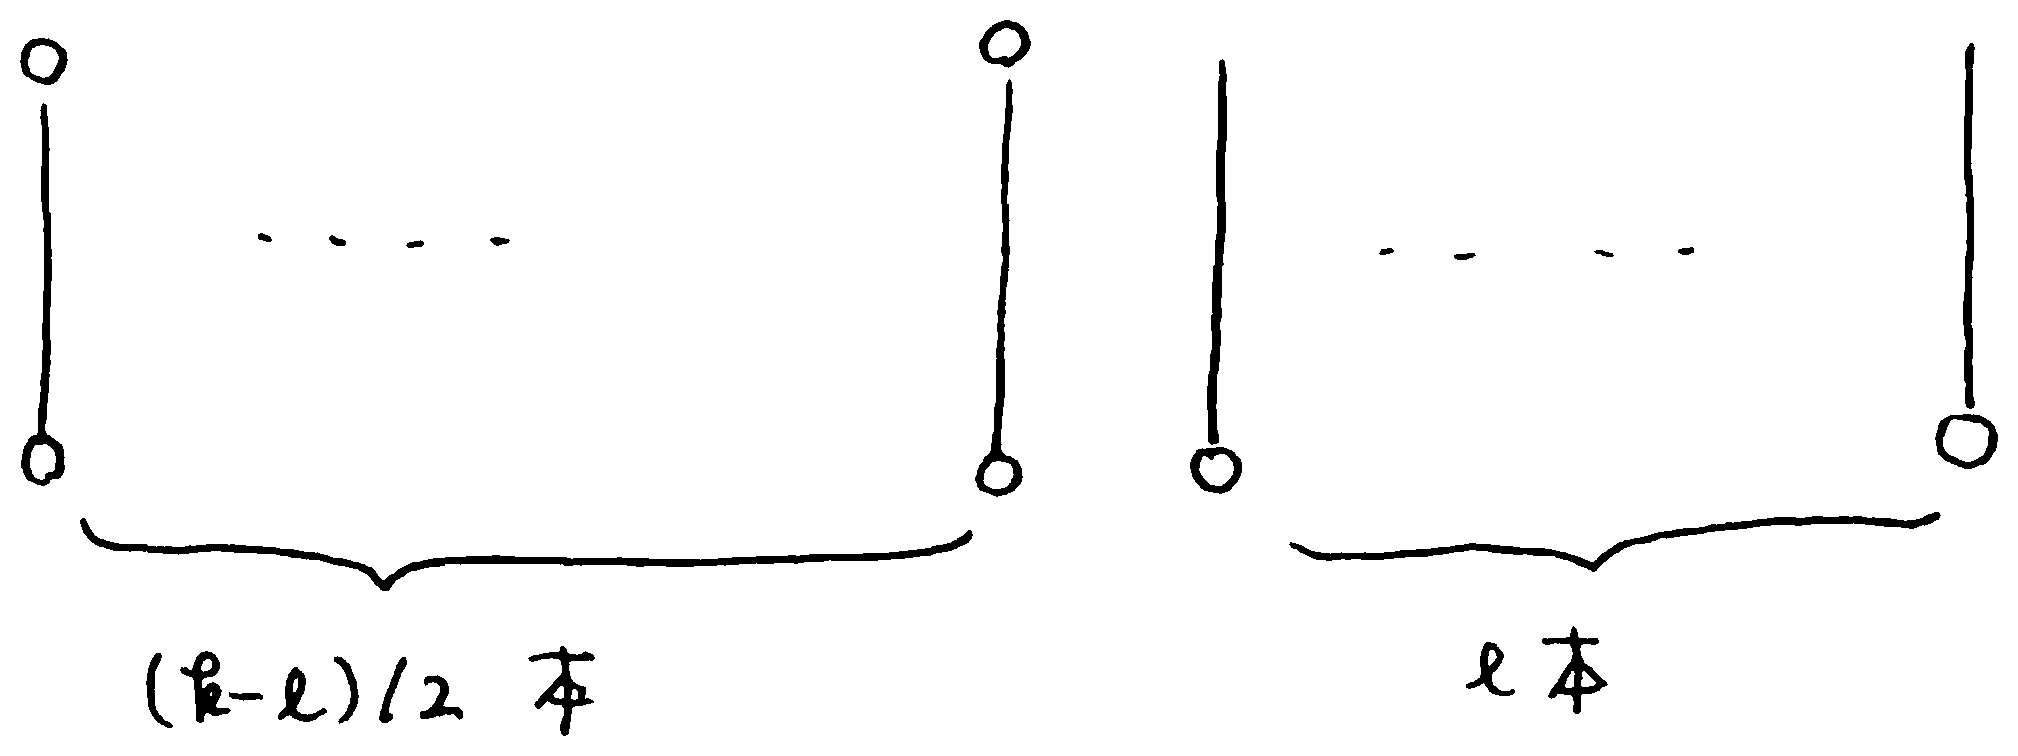
\includegraphics[width=0.60\linewidth]{fig_p70_a.png}
\end{center}

% ===== 原书 p.65 =====
实际上这可由归纳法证明。
\[
\begin{aligned}
\Bigl(\frac{\partial}{\partial j}\Bigr)^{k+1}e^{\frac12 j^2}
&=\Bigl\{\frac{\partial}{\partial j}\Bigl(\sum_{l=0}^k a_{kl}j^l\Bigr)
+\Bigl(\sum_{l=0}^k a_{kl}j^l\Bigr)\cdot j\Bigr\}e^{\frac12 j^2}\\
&=\Bigl(\sum_{l=0}^k a_{kl}\,l\,j^{l-1}
+\sum_{l=0}^k a_{kl}j^{l+1}\Bigr)e^{\frac12 j^2}
\end{aligned}
\]
成立，故只需证明$a_{k+1,l}=(l+1)a_{k,l+1}+a_{k,l-1}$即可。第一项是第$(k+1)$个顶点成为闭边的情形数，第二项是成为开边的情形。又，用此$a_{kl}$，经简单的 scale 变换得
\[
\Bigl(\frac{\partial}{\partial j}\Bigr)^k e^{j^2/(2\kappa)}
=\Bigl(\sum_{l=0}^k a_{kl}j^l\kappa^{-(k+l)/2}\Bigr)e^{j^2/(2\kappa)}.
\]
这里令$l=0$，即得下述定理。

\begin{theorem}[Wick]
\[
\frac{\langle x^k\rangle}{\langle 1\rangle}=a_{k,0}\kappa^{-k/2}.
\]
\end{theorem}

其中$a_{k0}$是把编号$1\sim k$的顶点两两配对、不剩余地全部连接起来的方法数。

这是使用 Feynman 图时的基本定理。它有许多 version，下面考虑顶点着色的版本。

设$x={}^t(x_1,\dots,x_r)$为$r$维列向量，$Q=(q_{ij})$为可逆对称矩阵。对$I=(a_1,\dots,a_r)\in\N^r$、$|a|=\sum_{i=1}^r a_i$，记$x^I=x_1^{a_1}\cdots x_r^{a_r}$。考虑求
\[
\langle x^I\rangle=\int_{\R^r}x^I\exp\Bigl(-\frac12{}^tXQX\Bigr)\,dx_1\cdots dx_r
\]
的值。设$J={}^t(y_1,\dots,y_r)$。因
\[
-\frac12{}^tXQX+{}^tJX
=-\frac12{}^t(X+Q^{-1}J)Q(X+Q^{-1}J)+\frac12{}^tJQ^{-1}J,
\]
故令$P=Q^{-1}=(p_{ij})$、$\partial^{|I|}/\partial y^I
=(\partial/\partial y_1)^{a_1}\cdots(\partial/\partial y_r)^{a_r}$，则
\[
\begin{aligned}
\langle x^I\rangle
&=\frac{\partial^{|I|}}{\partial y^I}
\int\exp\Bigl(-\frac12{}^tXQX+{}^tJX\Bigr)\,dX\Big|_{J=0}\\
&=\langle 1\rangle
\Bigl(\frac{\partial^{|I|}}{\partial y^I}\exp\Bigl(\frac12{}^tJPJ\Bigr)\Big|_{J=0}\Bigr).
\end{aligned}
\]

% ===== 原书 p.66 =====
其次，取$K=(b_1,\dots,b_r)\in\N^r$，则$(\partial^{|I|}/\partial y^I)\exp(\frac12{}^tJPJ)$中$y^K\exp(\frac12{}^tJPJ)$的系数$a_{IK}$如下计算。先准备颜色$1\sim r$。设$|I|=l$、$|K|=m$，准备$l$个 type I 的顶点并编上$1\sim l$的号。准备$m$个 type II 的顶点，不给它们编号（type II 看作前例中开边虚拟连接的对方）。把这$(l+m)$个顶点两个一组用边连接，考虑连接方式；其中不允许 type II 之间相连的情形，其余连接方式都考虑。进而给 type I、type II 的顶点涂上$1\sim r$的颜色，使 type I 中各种颜色的个数为$a_1,\dots,a_r$，type II 中各种颜色的个数为$b_1,\dots,b_r$。这样得到的着色图全体记作$\Gamma$。对$G\in\Gamma$，定义$G$的权为$w(G)=\prod_{e\in G}p_e$。这里，对$G$的边$e$，若其两端点的颜色为$s_1,s_2$，则定义$p_e=p_{s_1,s_2}$。此时下述定理成立。

\begin{theorem}[Wick 定理的着色版本]
\[
a_{IK}=\sum_{G\in\Gamma}w(G).
\]
\end{theorem}

特别地，当$K=0$时，令
\[
\Gamma_I=\left\{\begin{array}{l}
\text{将 $|I|$ 个带编号的顶点 $1,\dots,l$ 涂上颜色 $1,\dots,r$，使各颜色的个数为 $a_1,\dots,a_r$，}\\[2pt]
\text{并把它们两个一组、不剩余地用边连接成的图形}
\end{array}\right\},
\]
则
\[
\frac{\langle x^I\rangle}{\langle 1\rangle}=a_{I,0}=\sum_{G\in\Gamma_I}w(G)
\]
给出。

下面转向矩阵模型。把上述想法应用于$n\times n$ Hermitian 矩阵全体所成的向量空间$H_n$，以及其上的二次形式$Q(X)=\frac12\tr(X\Lambda X)$（$X\in H_n$）。其中$\Lambda=\operatorname{diag}(\lambda_1,\dots,\lambda_n)$（$\lambda_i\in\R_+$）。令$X=(x_{ij})$，则
\[
Q(X)=\frac12\sum_{i,j}\frac{\lambda_i+\lambda_j}{2}|x_{ij}|^2.
\]

% ===== 原书 p.67 =====
这里，把$x_{ij}$（$i\neq j$）看作复变量，则$x_{ij}=\bar{x}_{ji}$。把$x_{ii}$看作实变量。$H_n$上的测度$dX$定义为$dX=\prod_{i,j}dx_{ij}$。对$I=(i_1,\dots,i_k)$、$J=(j_1,\dots,j_k)$，置$x_{IJ}=x_{i_1j_1}\cdots x_{i_kj_k}$。考虑求
\[
\langle x_{IJ}\rangle=\int x_{IJ}\exp\Bigl(-\frac12\tr(X\Lambda X)\Bigr)\,dX
\]
的值。与前面的论述同样，
\[
\langle x_{IJ}\rangle
=\frac{\partial^k}{\partial y_{IJ}}\exp\Bigl(-\frac12\tr(J\Lambda^{-1}J)\Bigr)\Big|_{J=0}
\]
给出。

\transnote{上式右端照原文印出：指数中为$-\frac12\tr(J\Lambda^{-1}J)$，且右端没有因子$\langle1\rangle$。这与前页相应公式的符号及写法都不一致，疑为原书排印之误。}

这里取$J=(y_{ij})\in H_n\cong\C^{n(n-1)/2}\times\R^n$的坐标$y_{ij}\in\C$（$i<j$）、$y_{ii}\in\R$，看作$n(n-1)/2$个复变量、$n$个实变量的函数。按着色版本时的表示法，准备$(i,j)$（$i,j=1,\dots,n$）这$n^2$个颜色即可；而由二次形式$Q(X)$确定的对称矩阵的逆矩阵$P=(P_{(ij),(i'j')})$为
\[
p_{(i,i),(i,i)}=\frac{1}{\lambda_i},\qquad
p_{(i,j),(j,i)}=\frac{2}{\lambda_i+\lambda_j},\qquad(i\neq j),
\]
其余成分为$0$。

\transnote{此式左端原书印作小写$p$，与上一句所定义的矩阵$P$大小写不一致。译本照原文印出。}

由此，用图表示时，可以不给顶点涂$(i,j)$色，而对每个顶点给以下这样的着色箭头。

\begin{center}
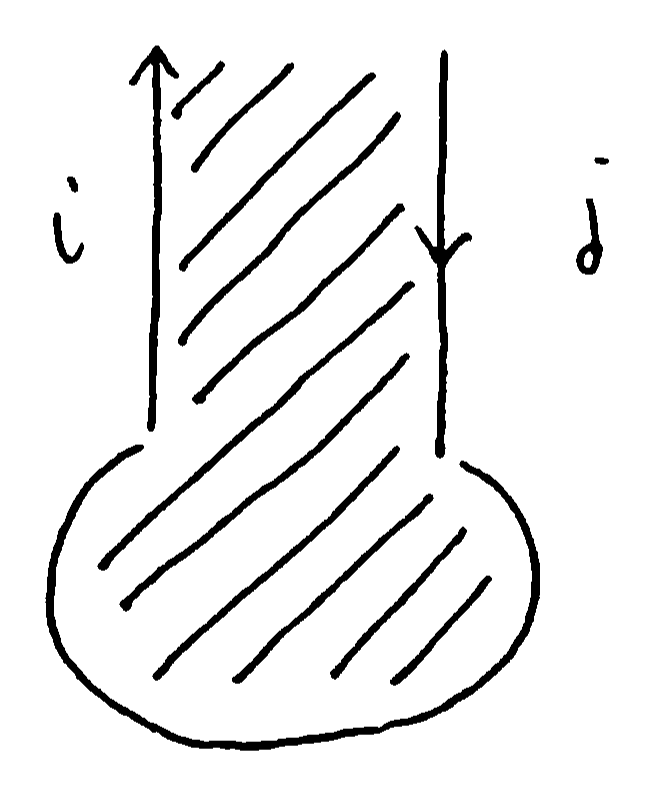
\includegraphics[width=0.26\linewidth]{fig_p73_a.png}
\end{center}

当然，考虑给顶点编号时，也对应于考虑带有上述着色箭头并且已编号的顶点。

\begin{center}
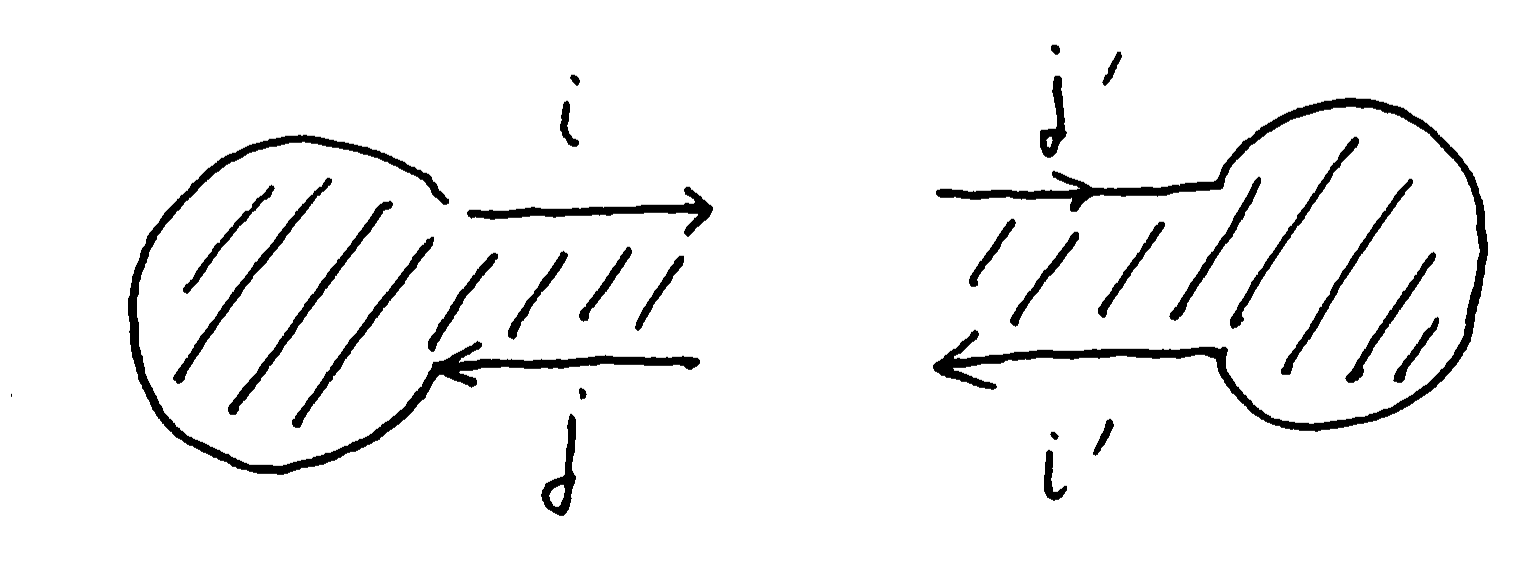
\includegraphics[width=0.62\linewidth]{fig_p73_b.png}
\end{center}

% c10 —— §4.2 作为 Lagrangian 微扰论的 Feynman 图；§4.3 与模空间相交理论的关系（原书 p.68–75）
% 负责：trans-e

% ===== 原书 p.68 =====
此时，两个顶点$(i,j),(i',j')$对应的$P$的分量不为$0$，只在如上图那样箭头与颜色的组合无矛盾地相接时才出现。此时，若定义这个图$G_{ij}$的权为
\[
w(G_{ij})=\frac{2}{\lambda_i+\lambda_j},
\]
则它与前述着色版本的权一致。设$I=(i_1,\dots,i_k)$，$J=(j_1,\dots,j_k)$。

\begin{center}
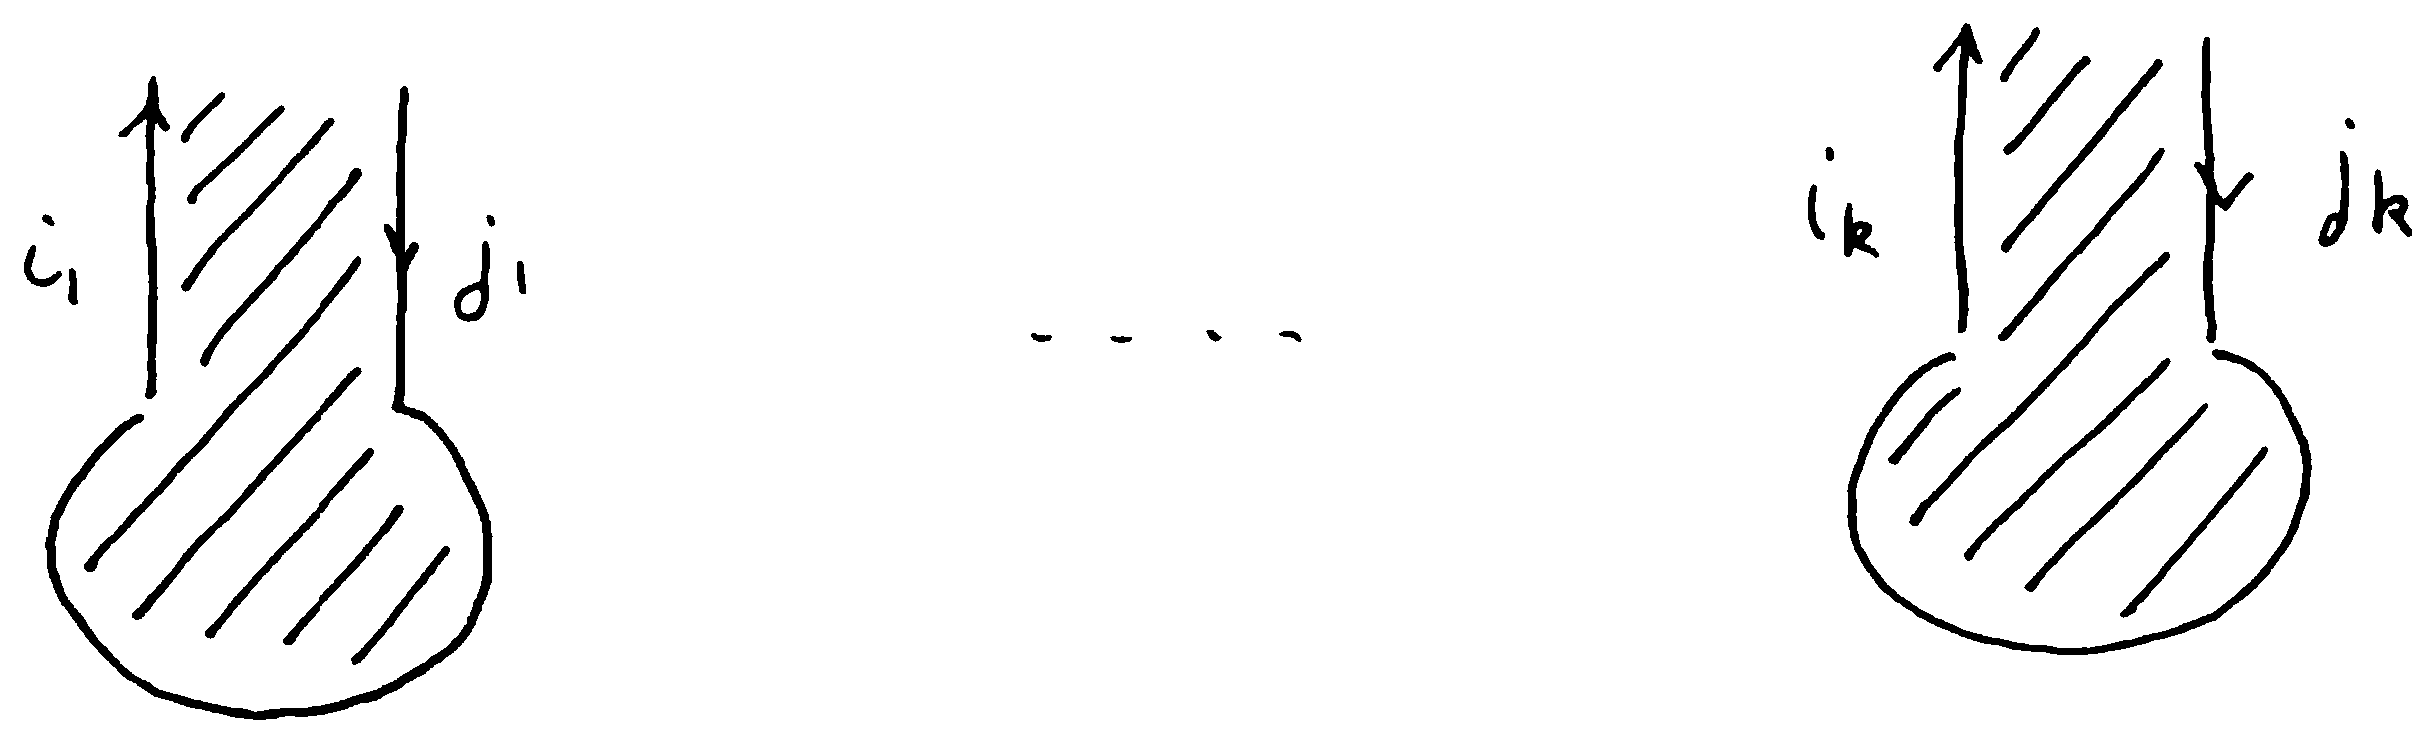
\includegraphics[width=0.56\linewidth]{fig_p74_a.png}
\end{center}

令
\[
\mathcal{A}(I,J)=\{\text{如上所述把 unit 两个一组无矛盾地组合起来所得的图形的全体}\},
\]
并对$\Gamma\in\mathcal{A}(I,J)$定义$w(T)=\prod_{e\in\Gamma}w(e)$。这里$e$是$\Gamma$的边，$w(e)$是先定义好的权。

\transnote{上式左端原书印作$w(T)$，而下文讨论的对象是$\Gamma$，$T$疑为$\Gamma$的排印之误。译本照原文印出。}

\begin{theorem}
\[
\frac{\langle x_{IJ}\rangle}{\langle 1\rangle}
=\sum_{\Gamma\in\mathcal{A}(I,J)}w(\Gamma).
\]
\end{theorem}

\subsection{Lagrangian 微扰论及其 Feynman 图}

以下暂且不论积分的收敛性。对充分小的$t$，把
\[
\langle\exp(tx^3/6)\rangle=\int\exp\Bigl(-\frac{\kappa}{2}x^2+\frac{t}{6}x^3\Bigr)\,dx
\]
按$t$展开，得$\sum_{i=0}^{\infty}\langle\frac{x^{3m}}{6^m m!}\rangle t^m$。把这个系数与三价图

\transnote{上式求和号下标原书印作$i=0$，而被求和的项中出现的指标是$m$，$i$疑为$m$的排印之误。译本照原文印出。}

% ===== 原书 p.69 =====
联系起来数吧。现在固定满足$2e=3v$的自然数$e,v$。
\[
\begin{aligned}
&\#\{\text{边、顶点都已编号，边数 $=e$、顶点数 $=v$ 的三价图}\}\times6^v\\
&\quad=\#\{\text{边、顶点都已编号，且从各顶点伸出的边再标上 $1\sim3$ 的号，}\\
&\qquad\qquad\text{边数 $=e$、顶点数 $=v$ 的三价图}\}\\
&\quad=\#\{\text{把 $(i,1)\sim(1,3)$（$i=1,\dots,v$）这 $3v$ 个顶点两个一组不剩余地}\\
&\qquad\qquad\text{配对的配法}\}\times e!\\
&\quad=e!\,\frac{\langle x^{3v}\rangle}{\langle 1\rangle}\kappa^e
\end{aligned}
\]
这从上一节可以明白。

\transnote{上式中第三行的$(1,3)$依前后文与所附图形应作$(i,3)$，原书如此印出，译本照印。}

现在，对边与顶点都已编号的三价图$\Gamma$，把$\Aut(\Gamma)$定义为边、顶点的编号所成集合的自同构中保持图的连接方式不变者。此时，把$\Gamma$去掉编号后所得者记作$\mathrm{Supp}(\Gamma)$。固定$\mathrm{Supp}(\Gamma)$时，编号的替换有$e!v!$种。在编号的替换中把彼此可由$\Aut(\Gamma)$互相转移者视为同一，则编号了的三价图$\Gamma'$中满足$\mathrm{Supp}(\Gamma')$与$\mathrm{Supp}(\Gamma)$相同者的个数为$\dfrac{e!v!}{\Aut(\Gamma)}$。因此，令
\[
G_{e,v}=\{\Gamma\mid\text{边数 $=e$、顶点数 $=v$ 的三价图}\}
\]
则
\[
\sum_{\Gamma\in G_{e,v}}\frac{e!v!}{\Aut(\Gamma)}6^v
=e!\,\frac{\langle x^{3v}\rangle}{\langle 1\rangle}\kappa^e
\]
成立。因此
\[
\frac{\langle\exp(tx^3/6)\rangle}{\langle 1\rangle}
=\sum_{m=0}^{\infty}\sum_{\Gamma\in G_{e,m}}
\frac{\kappa^{-\frac32 m}}{\Aut(\Gamma)}t^m
\]
成立。进而考虑把$\Gamma$分解为连通分支。把$\Gamma$作为三价图写成
\[
\Gamma=(\Gamma_1^{(1)}\sqcup\cdots\sqcup\Gamma_{m_1}^{(1)})
\sqcup\cdots\sqcup
(\Gamma_1^{(s)}\sqcup\cdots\sqcup\Gamma_{m_s}^{(s)})
\]

% ===== 原书 p.70 =====
即分解为连通分支。这里$\Gamma_j^{(i)}$（$j=1,\dots,m_i$）是彼此同型的三价图，上述分解是按同型者归并的分组。此时
\[
\#\Aut(\Gamma)
=m_1!\cdots m_s!\#\Aut(\Gamma_1^{(1)})\cdots\#\Aut(\Gamma_1^{(s)})
\]
成立，故上式成为
\[
\prod_{\Gamma:\ \text{连通}}
\Bigl(\sum_{m=0}^{\infty}\Bigl(\frac{1}{\Aut(\Gamma)}\Bigr)^m
\frac{1}{m!}(\kappa^{-\frac32}t)^{m v(\Gamma)}\Bigr)
\]
成立。这里$v(\Gamma)$是$\Gamma$的顶点数。因此对两边取对数，得
\[
\log\Bigl(\frac{\langle\exp(tx^3/6)\rangle}{\langle 1\rangle}\Bigr)
=\sum_{\Gamma:\ \text{连通}}\frac{1}{\Aut(\Gamma)}
(\kappa^{-\frac32}t)^{v(\Gamma)}
\]
这样的等式。这称为关于 Feynman 图的展开。

在矩阵模型的情形也作同样的考察，就出现关于带状图的展开。把$f(X)$取为关于$X\in H_n$的函数，令
\[
\langle f(X)\rangle=\int_{H_n}f(X)\exp\Bigl(-\frac12\tr(\Lambda X^2)\Bigr)\,dX
\]
当$f(X)=\exp\bigl(\frac{t}{3}\tr(X^3)\bigr)$时，试把$\langle f(X)\rangle$关于$t$展开。计算$\langle\frac{1}{3^m m!}(\tr(X^3))^m\rangle$。由于$\tr(X^3)=\sum_{i,j,k}x_{ij}x_{jk}x_{ki}$，有
\[
(\tr(X^3))^m
=\sum_{(i_1,j_1,k_1),\dots,(i_m,j_m,k_m)}
(x_{i_1j_1}x_{j_1k_1}x_{k_1i_1})\cdots(x_{i_mj_m}x_{j_mk_m}x_{k_mi_m}).
\]
于是，对$I=(i_1,j_1,k_1),\dots,(i_m,j_m,k_m)\in\{1,\dots,r\}^{3m}$，记
\[
x_I=(x_{i_1j_1}x_{j_1k_1}x_{k_1i_1})\cdots(x_{i_mj_m}x_{j_mk_m}x_{k_mi_m}).
\]
现在把集合$G_I$定义为
\[
G_I=\{\text{把下方的顶点无矛盾地两个一组配对并贴合所得的图形}\}
\]

\transnote{上式及此后诸式中原书用$r$，而此处矩阵是$n$阶、颜色标号取自$1,\dots,n$；$r$疑沿袭前一节（$r$个变量）的记号，译本照原文印出。}

% ===== 原书 p.71 =====
这样来定义。

\begin{center}
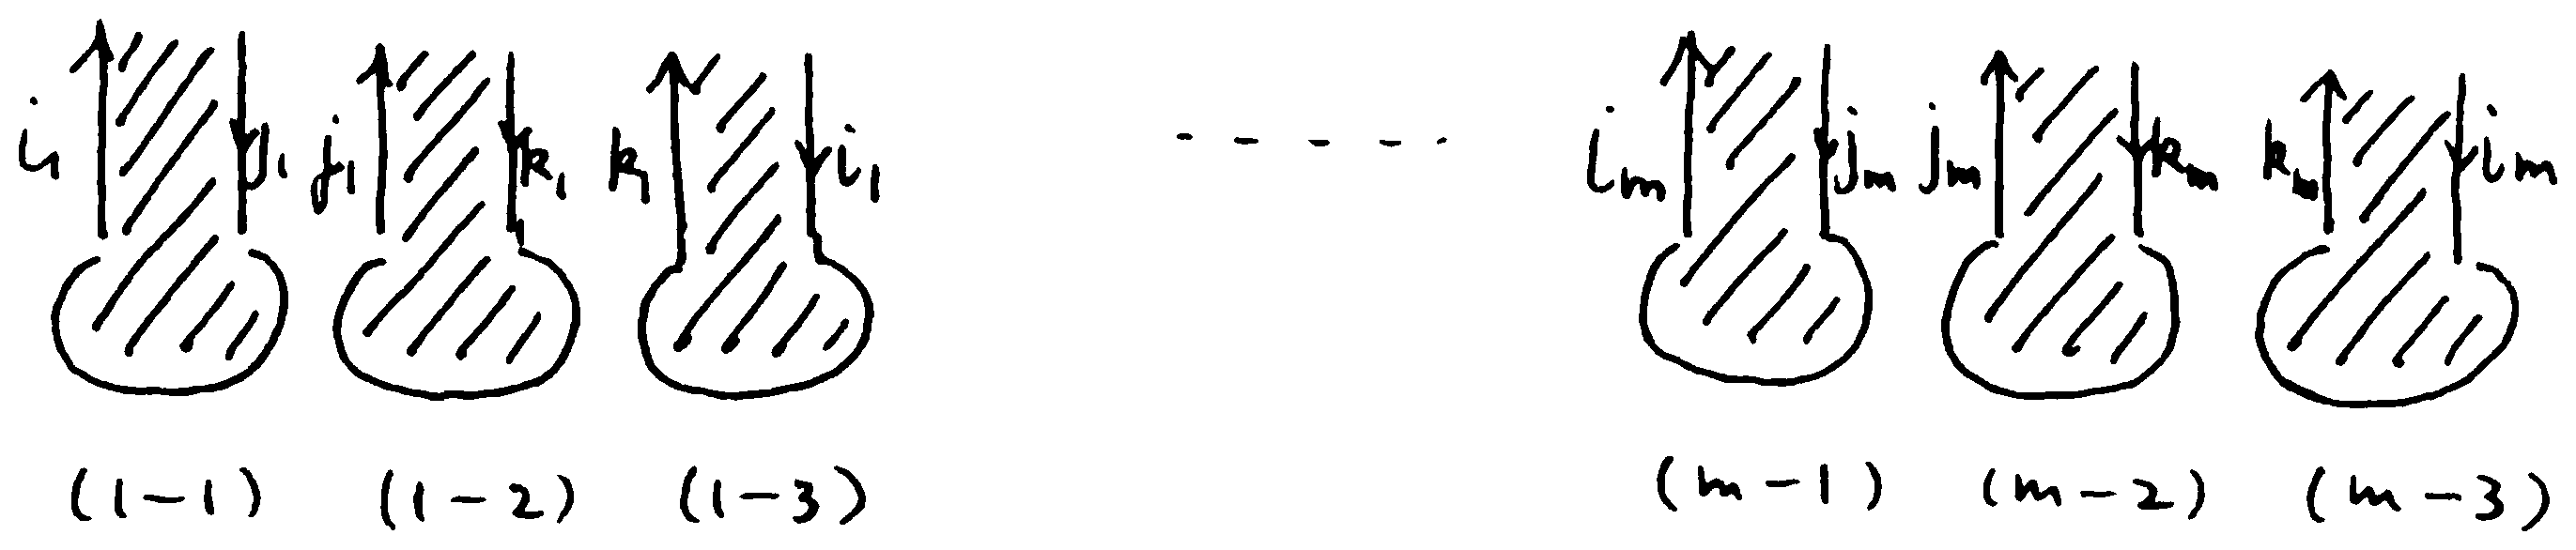
\includegraphics[width=0.80\linewidth]{fig_p77_a.png}
\end{center}

对$\Gamma\in G_I$，把$e\in\Gamma$取为一个组。这个组可看作带有两个边界的短带状图；把$i,j$取为$e$的两个边界上所附的编号，以$\tilde\lambda(e)=\lambda_i+\lambda_j$定义。此时由定理 4.3 得
\[
\frac{\langle x_I\rangle}{\langle 1\rangle}
=\sum_{\Gamma\in G_I}\prod_{e\in\Gamma}\frac{2}{\tilde\lambda(e)}.
\]
接着考虑把$G_I$重新分组。首先，对$\Gamma\in G_I$，如下构成三价带状图。把顶点$(1-1),(2-1),(3-1)$合成一个，考虑下图中那样的「三叉」图。

\transnote{上式中的$(2-1),(3-1)$与图中所附标号$(1-1),(1-2),(1-3)$不符，依文义应作$(1-1),(1-2),(1-3)$。原书如此印出，译本照印。}

\begin{center}
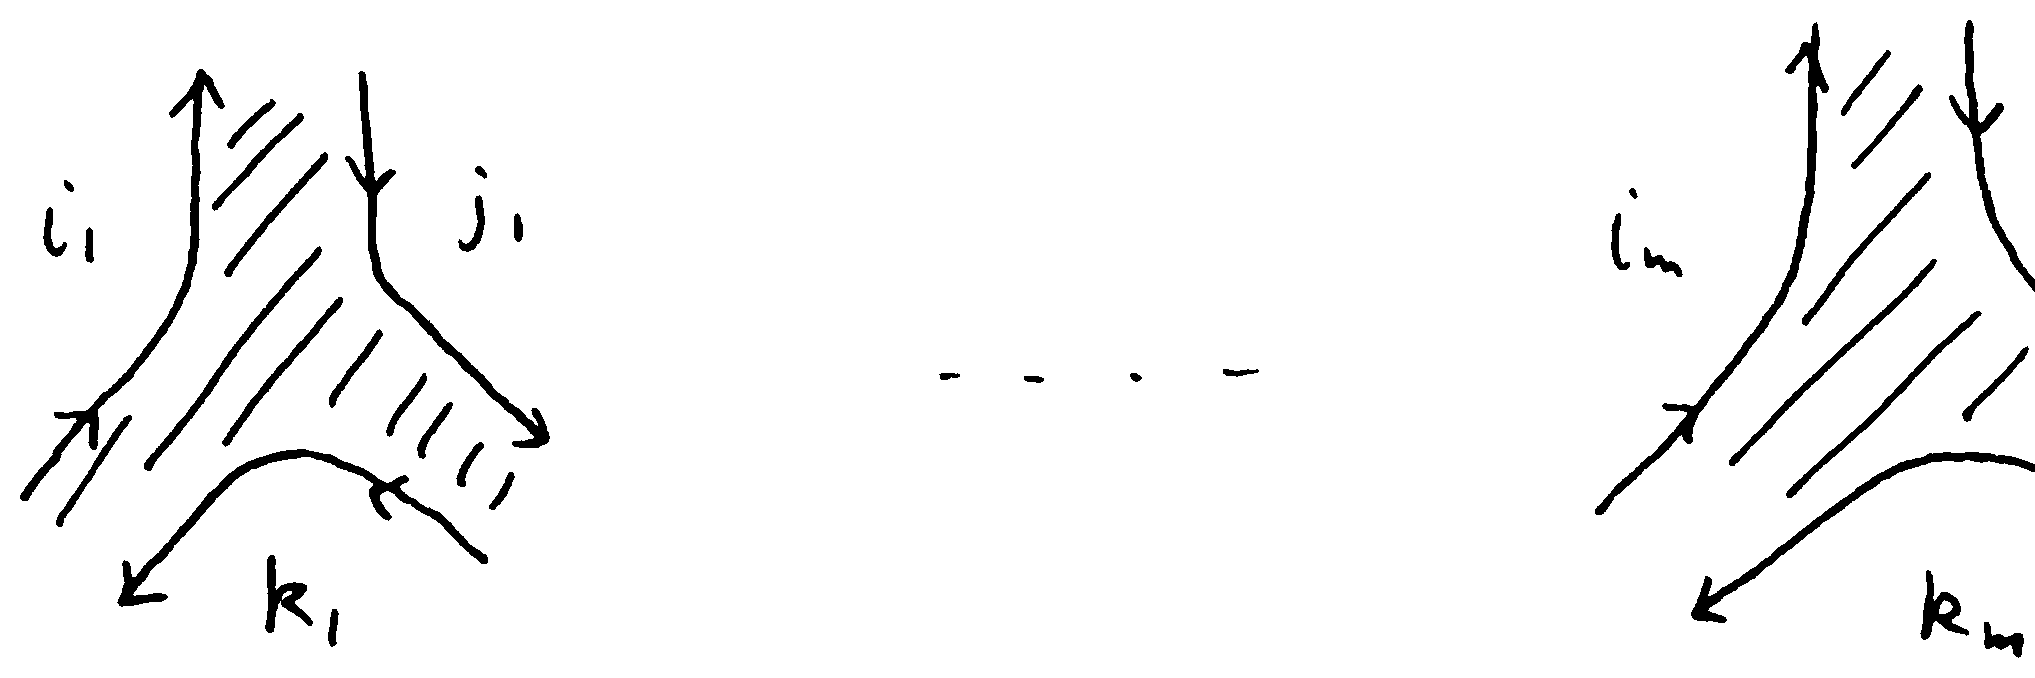
\includegraphics[width=0.78\linewidth]{fig_p77_b.png}
\end{center}

$\Gamma$是把各自的端不剩余且无矛盾地贴合的贴法，故按此把上述带状图贴合。这个带状图带有各顶点的编号与从该顶点伸出的三条边的编号。从一个点伸出的边的编号与给出带状图结构的循环次序相容。此外，边界上标有$1,\dots,r$的颜色。反之，考虑边界带颜色的三价带状图，其上的顶点、边有编号；从一点伸出的三条边的编号与 ribbon structre 相容，取 $1,2,3$。这样的组记为$\tilde\Gamma$。

% ===== 原书 p.72 =====
下面考察它。此时，在边的中点处切开时，就确定出$I=(i_1,j_1,k_1),\dots,(i_m,j_m,k_m)$这样一个$\{1,\dots,r\}^{3m}$的元素。称其为$\tilde\Gamma$的着色。若定义
\[
G_I^\psi=\left\{\begin{array}{l}
\text{边界上标有 $1,\dots,r$ 的颜色，其上的顶点、边的编号，以及从一点伸出的三条边的}\\
\text{ribbon structre 相容的 $1,2,3$ 的编号均已给出，且着色为 $I$ 的三价带状图}
\end{array}\right\},
\]
则忘记边的编号所得的映射$G_I^\psi\to G_I$是$e!:1$的映射。进而定义

\transnote{原文此处的 ribbon structure 印作 ribbon structre，上文（原书 p.71 末行）亦同，译本照原文印出。}
\[
G_\#^c=\left\{\begin{array}{l}
\text{边界上标有 $1,\dots,r$ 的颜色，其上的顶点与边的编号已给出的带状图}
\end{array}\right\},
\]
把$\coprod_IG_I^\psi\to G_\#^c$取为忘记从各顶点伸出的边的次序的映射，则它是$3^v:1$的映射。因此
\[
\begin{aligned}
\frac{\langle(\tr(X^3))^m\rangle}{3^m m!\langle 1\rangle}
&=\frac{1}{3^m m!}\sum_{I\in[1,r]^{3m}}\sum_{\Gamma\in G_I^\psi}
\prod_{e\in\Gamma}\frac{2}{\tilde\lambda(e)}\\
&=\frac{1}{3^m m!e!}\sum_{I\in[1,r]^{3m}}\sum_{\Gamma\in G_I}
\prod_{e\in\Gamma}\frac{2}{\tilde\lambda(e)}\\
&=\frac{1}{m!e!}\sum_{\Gamma\in G_\#^c}\prod_{e\in\Gamma}\frac{2}{\tilde\lambda(e)}
\end{aligned}
\]
成立。对$\Gamma\in G_\#^c$，把$\Aut^c(\Gamma)$定义为$\Gamma$的保持着色的自同构，并令
\[
G^c=\{\text{边界带颜色的带状图，且不考虑顶点、边的编号}\},
\]
则上式写作
\[
\sum_{\Gamma\in G^c}\frac{1}{\Aut^c(\Gamma)}\prod_{e\in\Gamma}\frac{2}{\tilde\lambda(e)}.
\]
现在乘上$t^m$并对$m$求和；为明示$m$，把$G^c,G_\#^c$分别写作$G_m^c,G_{\#,m}^c$。这里$m$是顶点数。

% ===== 原书 p.73 =====
\begin{theorem}
\[
\frac{\langle\exp(\frac{t\tr(X^3)}{3})\rangle}{\langle 1\rangle}
=\sum_{m=0}^{\infty}
\Bigl(\sum_{\Gamma\in G_m^c}\frac{1}{\Aut^c(\Gamma)}
\prod_{e\in\Gamma}\frac{2}{\tilde\lambda(e)}\Bigr)t^m
\]
\end{theorem}

下面考虑把$\Gamma$分解为 connceted component。把$\Gamma$分解为 connceted compoent，并把着色也包含在内按同型者归并，写成

\transnote{本段中原书把 connected 误排为 connceted，把 component 误排为 compoent，译本照原文印出。}

\[
\Gamma=(\Gamma_1^{(1)}\sqcup\cdots\sqcup\Gamma_{m_1}^{(1)})
\sqcup\cdots\sqcup
(\Gamma_1^{(s)}\sqcup\cdots\sqcup\Gamma_{m_s}^{(s)})
\]
则
\[
\Aut^c(\Gamma)=m_1!\cdots m_s!
\#\Aut^c(\Gamma_1^{(1)})^{m_1}\times\cdots\times
\#\Aut^c(\Gamma_1^{(s)})^{m_s},
\]
故令$G_m^{c0}=\{\Gamma\in G_m^c\mid\Gamma\text{ 连通}\}$，得
\[
\begin{aligned}
&\sum_{m=0}^{\infty}\Bigl(\sum_{\Gamma\in G_m^c}\frac{1}{\Aut^c(\Gamma)}
\prod_{e\in\Gamma}\frac{2}{\tilde\lambda(e)}\Bigr)t^m\\
&\quad=\prod_{m=1}^{\infty}\prod_{\Gamma\in G_m^{c0}}
\Bigl(\sum_{k=0}^{\infty}\frac{1}{k!}
\Bigl(\frac{1}{\Aut^c(\Gamma)}\prod_{e\in\Gamma}\frac{2}{\tilde\lambda(e)}\Bigr)^k
t^{km}\Bigr)
\end{aligned}
\]
成立。因此
\[
\log\Bigl(\frac{\langle\exp(\frac{t\tr(X^3)}{3})\rangle}{\langle 1\rangle}\Bigr)
=\sum_{m=1}^{\infty}\sum_{\Gamma\in G_m^{c0}}
\Bigl(\frac{1}{\Aut^c(\Gamma)}\prod_{e\in\Gamma}\frac{2}{\tilde\lambda(e)}\Bigr)t^m
\]
成立。

令$G_{\#m}^{c0}=\{\Gamma\in G_{\#m}^c\mid\Gamma\text{ 连通}\}$，则
\[
\sum_{\Gamma\in G_m^{c0}}\frac{1}{\Aut^c(\Gamma)}
\prod_{e\in\Gamma}\frac{2}{\tilde\lambda(e)}
=\sum_{\Gamma\in G_{\#m}^{c0}}\frac{1}{m!e!}
\prod_{e\in\Gamma}\frac{2}{\tilde\lambda(e)}
\]
成立。进而令
\[
G_{\#m,n}^{b0}=\left\{\begin{array}{l}
\text{带有 $n$ 个已编号的边界、边与顶点均已编号的连通带状图，且顶点数 $=m$}
\end{array}\right\},
\]
\[
G_{m,n}^{b0}=\left\{\begin{array}{l}
\text{带有 $n$ 个已编号的边界的带状图，且顶点数 $=m$}
\end{array}\right\}
\]

% ===== 原书 p.74 =====
并这样来定义。对应边界$1,\dots,n$引入新的变量$u_1,\dots,u_n$，对$\Gamma\in G_{m,n}^{b0}$的边$e\in\Gamma$，以$u_i+u_j$定义$\tilde u(e)$。进而对$J=(j_1,\dots,j_n)\in[1,r]^n$以及$f(u_1,\dots,u_n)\in\C[u_1,\dots,u_n]$，定义$f(u)^J=f(\lambda_{j_1},\dots,\lambda_{j_n})\in\C[\lambda_1,\dots,\lambda_r]$。于是
\[
\begin{aligned}
\sum_{\Gamma\in G_{\#m}^{c0}}\frac{1}{m!e!}
\prod_{e\in\Gamma}\frac{2}{\tilde\lambda(e)}
&=\sum_n\sum_{\Gamma\in G_{\#m,n}^{b0},\ J\in[1,r]^n}
\frac{1}{n!m!e!}\Bigl(\prod_{e\in\Gamma}\frac{2}{\tilde u(e)}\Bigr)^J\\
&=\sum_n\sum_{\Gamma\in G_{m,n}^{b0},\ J\in[1,r]^n}
\frac{1}{n!\Aut(\Gamma)}\Bigl(\prod_{e\in\Gamma}\frac{2}{\tilde u(e)}\Bigr)^J
\end{aligned}
\]
成立。归纳起来，

\begin{theorem}
\[
\log\Bigl(\frac{\langle\exp(\frac{t\tr(X^3)}{3})\rangle}{\langle 1\rangle}\Bigr)
=\sum_{n,m}t^m\sum_{\Gamma\in G_{m,n}^{b0},\ J\in[1,r]^n}
\frac{1}{n!\Aut(\Gamma)}\Bigl(\prod_{e\in\Gamma}\frac{2}{\tilde u(e)}\Bigr)^J
\]
\end{theorem}

\subsection{与模空间相交理论的关系}

把现在的定理与模空间的相交理论合起来思考。type$(g,n)$的三价带状图的顶点数$=-4+4g+2n$，故代入前一章的 main identity
\[
\sum_{d_1+\cdots+d_n=3g-3+n}
\langle\tau_{d_1},\dots,\tau_{d_n}\rangle
\prod_{i=1}^{n}\frac{(2d_i-1)!!}{u_i^{2d_i+1}}
=\sum_{\Gamma\in G_{m,n}^{b0}}\frac{2^{-m}}{\Aut(\Gamma)}
\prod_{e\in\Gamma}\frac{2}{\tilde u(e)}
\]
得
\[
\begin{aligned}
&\log\Bigl(\frac{\langle\exp(\frac{\tr(X^3)}{6})\rangle}{\langle 1\rangle}\Bigr)\\
&\quad=\sum_n\sum_{d_1,\dots,d_n}\langle\tau_{d_1},\dots,\tau_{d_n}\rangle
\sum_{J\in[1,r]^n}\frac{1}{n!}
\Bigl(\prod_{i=1}^{n}\frac{(2d_i-1)!!}{u_i^{2d_i+1}}\Bigr)^J
\end{aligned}
\]
成立。这里约定：当不存在满足$\sum_{i=1}^n d_i=3g-3+n$的$g$时，$\langle\tau_{d_1},\dots,\tau_{d_n}\rangle=0$。

\transnote{上一式的左端（含$\log$的式子），原书印作$\exp(\tr(X^3)/6)$，指数中不含$t$；而定理 4.5 中同一位置印作$\exp(t\tr(X^3)/3)$。此处照原文印出。}

作变量变换
\[
t_d=\sum_{i=1}^{n}\frac{(2d-1)!!}{\lambda_i^{2d+1}},
\]
则上式成为
\[
\begin{aligned}
&\sum_{n=0}^{\infty}\sum_{d_1,\dots,d_n}\frac{1}{n!}
\prod_{i=1}^{n}t_{d_i}\langle\tau_{d_1}\cdots\tau_{d_n}\rangle\\
&\quad=\sum_{m_i\ge0}\frac{1}{m_0!\cdots m_s!}
t_0^{m_0}\cdots t_s^{m_s}\langle\tau_0^{m_0}\cdots\tau_s^{m_s}\rangle
\end{aligned}
\]
而它在形式上可写作
\[
\langle\exp(t_0\tau_0)\exp(t_1\tau_1)\cdots\rangle
=\Bigl\langle\exp\Bigl(\sum_{i\ge0}t_i\tau_i\Bigr)\Bigr\rangle.
\]


% ===== 原书 p.75 =====
\begin{theorem}
在变量变换$t_d=\sum_{i=1}^{n}\frac{(2d-1)!!}{\lambda_i^{2d+1}}$之下，
\[
\log\Bigl(\frac{\langle\exp(\frac{\tr(X^3)}{6})\rangle}{\langle 1\rangle}\Bigr)
=\Bigl\langle\exp\Bigl(\sum_{i\ge0}t_i\tau_i\Bigr)\Bigr\rangle.
\]
\end{theorem}

% c11 —— §5 KP 方程理论概要；§5.1–§5.3（原书 p.76–83，末段延伸至 p.84 页首收尾）
% 负责：trans-f

% ===== 原书 p.76 =====
\section{KP 方程理论概要}

本节讲述 KP 方程理论的概要，但主要内容是佐藤方程以及用 Schur 函数展开 $\tau$ 函数。叙述按以下顺序进行。（更详细的文献举 [Sa]。）

\begin{enumerate}[label=\arabic*.,leftmargin=2.4em,itemsep=5pt,topsep=5pt]
\item 构造一个线性微分方程 $Wf=0$，使给定的 $d$ 维有限维函数空间 $V$ 为其解空间。这里 $W$ 是 rank 为 $d$ 的线性微分算子。$\dim=d$ 的向量空间 $V$ 的全体，与 rank 为 $d$ 的微分算子大致成 $1:1$ 对应。（若限制在 Wronskian 处处不为零的范围内，则是 $1:1$。）

\item 在 $\C[x]$ 内 $\dim=d$ 的向量空间全体所成的 Grassmann variety $Grass(d)$ 中，考虑一个特殊的流。它由与 $\partial=\frac{d}{dx}$ 可交换的线性算子中的幂零元素全体 $Z_n(\partial)$ 作为单参数子群生成。$Z_n(\partial)=\partial\C[[\partial]]$，这在拓扑上由 $\partial,\partial^2,\dots$ 生成。也就是由
\[
\{\exp(z)\in\Aut(Grass(d))\mid z\in Z_n(\partial)\}
\]
定出的流。设 $V\in Grass(d)$，把与 $\exp(z)V$ 对应的 rank $d$ 微分算子记作 $W(z,V)$。此时该微分算子的系数，经由 $V$ 的 Pluecker 坐标与 $z=t_1\partial+t_2\partial^2+\cdots$ 的坐标 $(t_1,t_2,\dots)$ 表示出来。也就是说，它由作为 Pluecker 坐标的母函数的 $\tau$ 函数表示。

\item 在 $Z_n(\partial)$ 上以 $z=t_1\partial+\cdots+t_N\partial^N$ 引入坐标 $t=(t_1,t_2,\dots,t_N)$，再考虑关于 $W=W(t,V)$ 的微分方程 $(S_d)$。这是以 $W$ 的系数为未知函数、关于 $t_i$ 的非线性偏微分方程。由此比较 2.\ 与 3.\ 可知：3.\ 的这个非线性偏微分方程具有由 $Grass(d)$ 参数化的解，且该解可写成 $\tau$ 函数。$(S_d)$ 是
\[
W=\partial^d+a_1\partial^{d-1}+\cdots+a_d
\]
的系数 $a_1,\dots,a_d$ 为未知函数、以 $t_1,\dots,t_N$ 为变量的偏微分方程。而对 $(S_d)$ 的解 $W$，$W\partial$ 是 $(S_{d+1})$ 的一种特殊形式的解。这样考虑 $(S_d)$ 关于 $d$ 的相容性时，若要同时处理所有的 $d$，自然的做法是推广为拟微分算子
\[
W=1+a_1\partial^{-1}+a_2\partial^{-2}+\cdots
\]
% ===== 原书 p.77 =====
的系数 $a_1,a_2,\dots$ 为未知函数的微分方程。在这一范畴中考虑，$(S_d)$ 便是 $a_{d+1}=a_{d+2}=\cdots=0$ 的解。一般地，要构造取值于 $1+\partial^{-1}\C[[\partial^{-1}]]$、无法在有限处截断的解，本质上必须构造不是 $Grass(d)$ 的并的 Grassmann variety。

\item 配合 Kontsevich 论文中的情形，作可以想到的那种电荷共轭变换，来表示 $\tau$ 函数。把 $\C[[x]]$ 看作 $\C[\partial]$-module 时，它同构于 $\C((\partial^{-1}))/\C[\partial]$。把 $\partial^{-1}$ 的记号改写为 $\xi$，把 $\C((\xi))/\C[\xi^{-1}]$ 看作 $\C[\partial]$-module。此时，对 $\C((\xi))$ 中满足适当条件的函数列 $f_1,f_2,\dots$ 写出 $\tau$ 函数。这时 $\tau$ 函数可用行列式写出。

\item 最后在本章末尾，用 Harish-Chandra 定理证明：具有矩阵积分表示的函数确实为 KP 方程的 $\tau$ 函数。
\end{enumerate}

\transnote{原书对本名的拼写不统一：§5.1 与 §5.3 的标题（原书 p.77、p.81）均作 GRASMANN，正文 p.76 作 Grassman、p.77 作 Grasmman、p.83 作 Gasmman；此外把 Plücker 一律拼作 Pluecker，把 nilpotent 拼作 niponent。译本统一写作 Grassmann variety 与 Pluecker 坐标；Pluecker 坐标即通行的 Plücker 坐标。}

\transnote{原书此处作「荷電共役変換」，而 §0（原书 p.2）作「共役荷電変換」，二者同指电荷共轭变换。}

\subsection{Grassmann variety 与微分算子的对应}

设 $V$ 为 $\C$ 上可微函数的 $d$ 维子空间，$f_1,\dots,f_d$ 为 $V$ 的基；再设 $g$ 含于 $V$，则
\[
(*)\qquad
\det
\begin{pmatrix}
f_1 & \partial f_1 & \cdots & \partial^d f_1\\
f_2 & \partial f_2 & \cdots & \partial^d f_2\\
 & \cdots & \cdots & \\
f_d & \partial f_d & \cdots & \partial^d f_d\\
g & \partial g & \cdots & \partial^d g
\end{pmatrix}
\]
若 Wronskian
\[
W(f_1,\dots,f_d)=\det
\begin{pmatrix}
f_1 & \partial f_1 & \cdots & \partial^{d-1}f_1\\
\vdots & & & \vdots\\
f_d & \partial f_d & \cdots & \partial^{d-1}f_d
\end{pmatrix}
\]
不为 $0$，则把它看作关于 $g$ 的微分方程，即为 $d$ 阶线性微分方程，故其解与由 $f_1,\dots,f_d$ 张成的 $V$ 一致。把 $(*)$ 作余子式展开，得到
\[
\bigl[W(f_1,\dots,f_d)\partial^d+(\partial W(f_1,\dots,f_d))\partial^{d-1}+\cdots\bigr]g=0
\]

% ===== 原书 p.78 =====
于是除以 $W(f_1,\dots,f_d)$，得到 monic 微分方程
\[
\begin{gathered}
W=\frac{W(f_1,\dots,f_d)\partial^d+(\partial W(f_1,\dots,f_d))\partial^{d-1}+\cdots}{W(f_1,\dots,f_d)}\\
Wg=0
\end{gathered}
\]
此时 $W$ 只依赖于 $d$ 维子空间，故写作 $W=W(V,\partial)$。反之，rank $d$ 的线性微分算子有 $d$ 个独立解，由此可构成 $V$。在这个意义上，Wronskian 处处不为零的 $d$ 维向量空间 $V$ 与 $d$ 阶 monic 线性微分算子成 $1:1$ 对应。

\subsection{Grassmann variety 上的动力系统与 $\tau$ 函数的展开}

特别考虑含于 $\C[x]$ 的 $d$ 维子空间。这样的子空间全体记作 $Grass(d)$。$\C[x]$ 带有关于次数的滤过。保持该滤过且与 $\partial$ 交换的幂零线性映射全体，可等同于 $Z_n(\partial)=\partial\C[[\partial]]$。考虑前述的流 $\exp(z)$（$z\in Z_n(\partial)$），对 $V\in Grass(d)$，把与 $\exp(z)V\in Grass(d)$ 对应的微分算子记作 $W(z,V)$。写作 $z=t_1\partial+t_2\partial^2+\cdots$，把它看作 $t_1,t_2,\dots$ 的函数，记作 $(t,V)$。下面计算 $W(t,V)$。设 $V$ 的基为 $f_i=\sum_{j=0}^N a_{ij}x^j/j!$（$i=1,\dots,d$），令 $f_i(x,t)=\exp(z)f_i(x)$，则 $\exp(z)V$ 由 $f_1(x,t),\dots,f_d(x,t)$ 生成。试计算其 Wronskian 矩阵 $W(f_1(x,t),\dots,f_d(x,t))$。取 $1,x,x^2/2,\dots,x^N/N!$ 作为 $\C\oplus\C x\oplus\cdots\oplus\C x^N$ 的基，把 $f_1,\dots,f_d$ 与列向量 ${}^{t}(a_{i0},\dots,a_{iN})$ 等同起来。此时若用矩阵表示 $\partial$，则为
\[
\Lambda=
\begin{pmatrix}
0 & 1 & 0 & \cdots & 0\\
 & & \cdots & & \\
0 & 0 & \cdots & 0 & 1\\
0 & 0 & \cdots & 0 & 0
\end{pmatrix}
\]

% ===== 原书 p.79 =====
可写成如此。又，
\[
\begin{aligned}
\exp(x\Lambda)
\begin{pmatrix}
a_{i0}\\ \vdots\\ a_{iN}
\end{pmatrix}
&=
\begin{pmatrix}
1 & x & \frac{x^2}{2} & \cdots\\
0 & 1 & x & \cdots\\
 & & \cdots & \\
0 & 0 & \cdots & 0
\end{pmatrix}
\begin{pmatrix}
a_{i0}\\ \vdots\\ a_{iN}
\end{pmatrix}\\
&=
\begin{pmatrix}
f_i\\ \vdots\\ \partial^N f_i
\end{pmatrix}
\end{aligned}
\]
可写成如此。由此，
\[
\begin{aligned}
&\exp(t_1\Lambda+\cdots+t_N\Lambda^N)
\begin{pmatrix}
f_1 & f_2 & \cdots & f_d\\
\partial f_1 & \partial f_2 & \cdots & \partial f_d\\
 & \cdots & \cdots & \\
\partial^N f_1 & \partial^N f_2 & \cdots & \partial^N f_d
\end{pmatrix}\\
&\qquad=\exp\bigl((x+t_1)\Lambda+t_2\Lambda^2+\cdots+t_N\Lambda^N\bigr)
\begin{pmatrix}
a_{10} & \cdots & a_{d0}\\
 & \cdots & \\
a_{1N} & \cdots & a_{dN}
\end{pmatrix}\\
&\qquad=\exp\bigl((x+t_1)\Lambda+t_2\Lambda^2+\cdots+t_N\Lambda^N\bigr)\xi
\end{aligned}
\]
可以写成如此。这里 $\xi$ 是 $V$ 的 frame。
\[
\xi=
\begin{pmatrix}
a_{10} & \cdots & a_{d0}\\
 & \cdots & \\
a_{1N} & \cdots & a_{dN}
\end{pmatrix}
\]
由于 $x$ 必定以 $x+t_1$ 的形式出现，故在 $x=0$ 时求出即可。此时 Wronskian determinant 为
\[
\det
\begin{pmatrix}
f_1 & f_2 & \cdots & f_d\\
\partial f_1 & \partial f_2 & \cdots & \partial f_d\\
 & \cdots & \cdots & \\
\partial^{d-1}f_1 & \partial^{d-1}f_2 & \cdots & \partial^{d-1}f_d
\end{pmatrix}
=\det\bigl((I_d,0)\exp(t_1\Lambda+\cdots+t_N\Lambda^N)\xi\bigr)
\]

\transnote{原书把 $\exp(x\Lambda)$ 的最后一个行向量印作 $(0,0,\cdots,0)$；按 $\Lambda$ 的幂零 Jordan 块形状，该行末项应为 $1$。译文照原文排印。}

% ===== 原书 p.80 =====
成为如此。现引入新变量 $t_i=\frac{1}{i}\sum_{j=1}^N\lambda_j^i$，则
\[
\begin{aligned}
\exp(t_1\Lambda+\cdots+t_N\Lambda^N)
&=\prod_{i=1}^N\exp\Bigl(\lambda_i\Lambda+\frac{1}{2}\lambda_i^2\Lambda^2+\cdots+\frac{1}{N}\lambda_i^N\Lambda^N\Bigr)\\
&=\prod_{i=1}^N(1-\lambda_i\Lambda)^{-1}\\
&=\sum_{i=0}^N m_i(\lambda)\Lambda^i\\
&=
\begin{pmatrix}
1 & m_1 & m_2 & \cdots & m_N\\
0 & 1 & m_1 & \cdots & m_{N-1}\\
 & & \cdots & &
\end{pmatrix}
\end{aligned}
\]
这里 $m_i$ 是称作 complete monomial 的对称函数。对 $0\le i_1<i_2<\cdots<i_d$，用 Jacobi–Trudi 等式
\[
\det
\begin{pmatrix}
m_{i_1} & \cdots & m_{i_d}\\
m_{i_1-1} & \cdots & m_{i_d-1}\\
 & \cdots & \\
m_{i_1-d+1} & \cdots & m_{i_d-d+1}
\end{pmatrix}
=S_Y(\lambda_1,\dots,\lambda_N)
\]
变形 Wronskian。这里 $Y$ 是 Young tableau $Y=(i_d,i_{d-1},\dots,i_1)-(d-1,d-2,\dots,0)$，$S_Y$ 是关于 $\lambda_1,\dots,\lambda_N$ 的 Schur 对称函数。
\[
S_Y(t)=\frac{\det
\begin{pmatrix}
\lambda_1^{i_1} & \cdots & \lambda_1^{i_d}\\
\vdots & & \vdots\\
\lambda_m^{i_1} & \cdots & \lambda_m^{i_d}
\end{pmatrix}}{\prod_{i<j}(\lambda_i-\lambda_j)}
\]

\transnote{原书此处 $S_Y(t)$ 的分子末行为 $\lambda_m^{i_1},\dots,\lambda_m^{i_d}$，分母作 $\prod_{i<j}(\lambda_i-\lambda_j)$；而 $S_Y$ 通篇只用到 $\lambda_1,\dots,\lambda_N$，$m$ 未给出定义，疑为 $N$（或 $d$）之误。译文照原文排印。}
把 $S_Y$ 看作 $t=(t_1,\dots,t_N)$ 的函数时，写作 $S_Y(t)$。对 Young diagram $Y$，把 Pluecker 坐标 $\xi_Y$ 定义为
\[
\xi_Y=\det
\begin{pmatrix}
a_{1i_1} & \cdots & a_{di_1}\\
 & \cdots & \\
a_{1i_d} & \cdots & a_{di_d}
\end{pmatrix}
\]
则
\[
W(f_1(0,t),\dots,f_d(0,t))=\sum_Y S_Y(t)\xi_Y
\]

% ===== 原书 p.81 =====
可以写成如此。这里 $Y$ 跑遍纵横尺寸落在下图范围内的 Young tableau。
\begin{center}
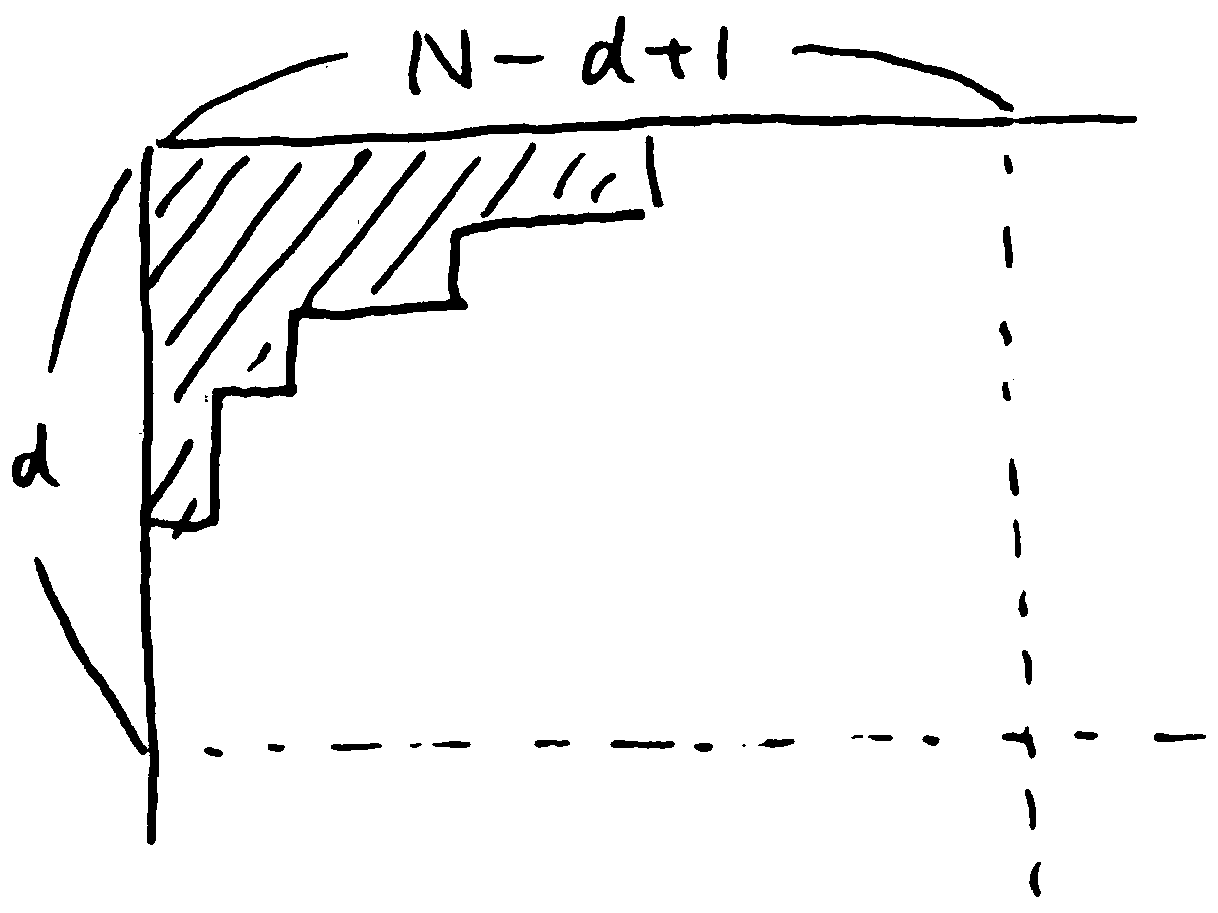
\includegraphics[width=0.62\linewidth]{fig_p87_a.png}
\end{center}
把 $W(f_1(0,t),\dots,f_d(0,t))$ 看作 $t$ 与 $\xi$ 的函数，称为 $\tau$ 函数。实际上，设对应的微分算子为 $W=W(t,V)=\partial^d+w_1\partial^{d-1}+w_2\partial^{d-2}+\cdots$，则存在某个 $P_i(\partial_t)=P_i\bigl(\frac{\partial}{\partial t_1},\dots,\frac{\partial}{\partial t_N}\bigr)$，使
\[
w_i=\frac{P_i(-\partial_t)\tau(t,\xi)}{\tau(t,\xi)}
\]
成立。（实际上 $P_i$ 是 complete monomial 的简单 modification。）也就是说，$W=W(t,V)$ 由 $\tau$ 函数表示。这里 $N$ 在形式上可以任意大，故 $\tau$ 可看作 $t_1,t_2,\dots$ 的函数。当然，若 $f_1,\dots,f_d\in\C\oplus\cdots\oplus\C x^N$，则 $\tau$ 实质上是 $t_1,\dots,t_N$ 的函数。若 $f_1,\dots,f_d\in\C[[x]]$，则 $\tau$ 是无穷多个变量 $t_1,t_2,\dots$ 的函数。

\subsection{佐藤方程与无穷维 Grassmann variety}

下面考虑 $W$ 所满足的微分方程。置 $z=t_1\partial+t_2\partial^2+\cdots$。由于 $W(t,V)$ 是作为消去 $\exp(z)f_1,\dots,\exp(z)f_d$ 的 monic $d$ 阶微分算子被刻画出来的，故
\[
W(t,V)\exp(z)f_i=0\qquad(i=1,\dots,d).
\]

\transnote{原书 p.81 此处印 $t_2\partial$，脱了平方；同一定义在 p.78 印作 $t_2\partial^2$，译文按 p.78 补出。}

\transnote{原书此句作「特徴付けられたのかから，」，在因果接续处有笔误（当作「特徴付けられたのだから，」），译文按因果关系处理。又，此处原书作 monomial $d$ 阶微分算子，与 p.78 的 monic 指同一意思，疑为笔误。}

两边对 $t_j$ 微分，得
\[
\Bigl(\frac{\partial W(t,V)}{\partial t_j}\exp(z)+W(t,V)\partial^j\exp(z)\Bigr)f_i=0\qquad(i=1,\dots,d)
\]
因此存在某个微分算子 $B_j(t,V)$，使
\[
(S_d)\qquad
\frac{\partial W(t,V)}{\partial t_j}+W(t,V)\partial^j=B_j(t,V)W(t,V)
\]

% ===== 原书 p.82 =====
成为如此。取 $W=\partial^d+w_1\partial^{d-1}+\cdots+w_d$ 时，这成为系数 $w_i=w_i(t_1,\dots,t_d)$ 关于 $t_i$ 的非线性偏微分方程。称之为佐藤方程，或称 KP 方程。综合以上可知：要得到佐藤方程的解，只须对 frame $\xi$，由 $\tau$ 函数 $\tau(t,\xi)$ 按 $(*)$ 式构造 $W$ 即可。对 $(S_d)$ 的解 $W$，$W\partial$ 是 $(S_{d+1})$ 的解。$(S_{d+1})$ 中满足 $w_{d+1}=0$ 者，正是这样得到的解全体。考虑这一点，则关于
\[
W=1+w_1\partial^{-1}+w_2\partial^{-2}+\cdots
\]
的方程
\[
(S)\qquad
\frac{\partial W(t,V)}{\partial t_j}+W(t,V)\partial^j=B_j(t,V)W(t,V)
\]
与 $w_{d+1}=w_{d+2}=\cdots=0$ 联立，把 $w_1,\dots,w_d$ 看作未知函数，所得的不是别的，正是 $(S_d)$。也就是说，令 $w_{d+1}=w_{d+2}=\cdots=0$，即可把 $(S_d)$ 的解看作 $(S)$ 的解。那么，具有无限多个 $w_1,w_2,\dots$ 的非平凡解应如何构造？取 $1,x,x^2/2!,\dots$ 作为 $\C[[x]]$ 的基，把其元素用列向量表示。把 $f_1,\dots,f_{d+1}\in\C[[x]]$ 并排所得的矩阵记作 $\xi$，考虑 $\xi$ 呈下述形状者。

\transnote{原书此页两处印「対いして」（「frame $\xi$ に対いして」「$(S_d)$ の解 $W$ に対いして」），多出的「い」为衍字（当作「対して」）；译文按原义译出。}
\[
\xi=(f_{d+1},\dots,f_1)=
\begin{pmatrix}
1 & 0 & \cdots & 0\\
a_{d+1,2} & 1 & \cdots & 0\\
a_{d+1,3} & a_{d,3} & \cdots & 0\\
 & \cdots & &
\end{pmatrix}
\]
再定义 $\xi'=(f'_d,\dots,f'_1)$，其中 $f'_1=\partial f_1,\dots,f'_d=\partial f_d$。也就是写成矩阵则
\[
\xi'=(f'_{d+1},\dots,f'_1)=
\begin{pmatrix}
1 & \cdots & 0\\
a_{d,3} & \cdots & 0\\
 & \cdots &
\end{pmatrix}
\]
成为如此。此时，$\tau(x,\xi')$ 关于 $S_Y$ 的系数 $\xi'_Y$ 与 $\tau(x,\xi)$ 关于 $S_Y$ 的系数 $\xi_Y$，在 Young tableau $Y$ 的深度不超过 $d$ 的范围内一致。回想 Young diagram 与 $0\le i_1<\cdots<i_{d+1}$ 的对应，即可明白。实际上，对 $0\le i_1<\cdots<i_{d+1}$ 相
% ===== 原书 p.83 =====
应的 Young diagram 深度不超过 $d$，也就是 $i_1=0$。考虑到第一行为 $(1,0,\dots,0)$，由 Pluecker 坐标定义中的 determinant 式即可立即看出。要妥善处理关于 $d$ 的相容性，把 frame $\xi$ 的行与列的原点按下图选取为好。
\begin{center}
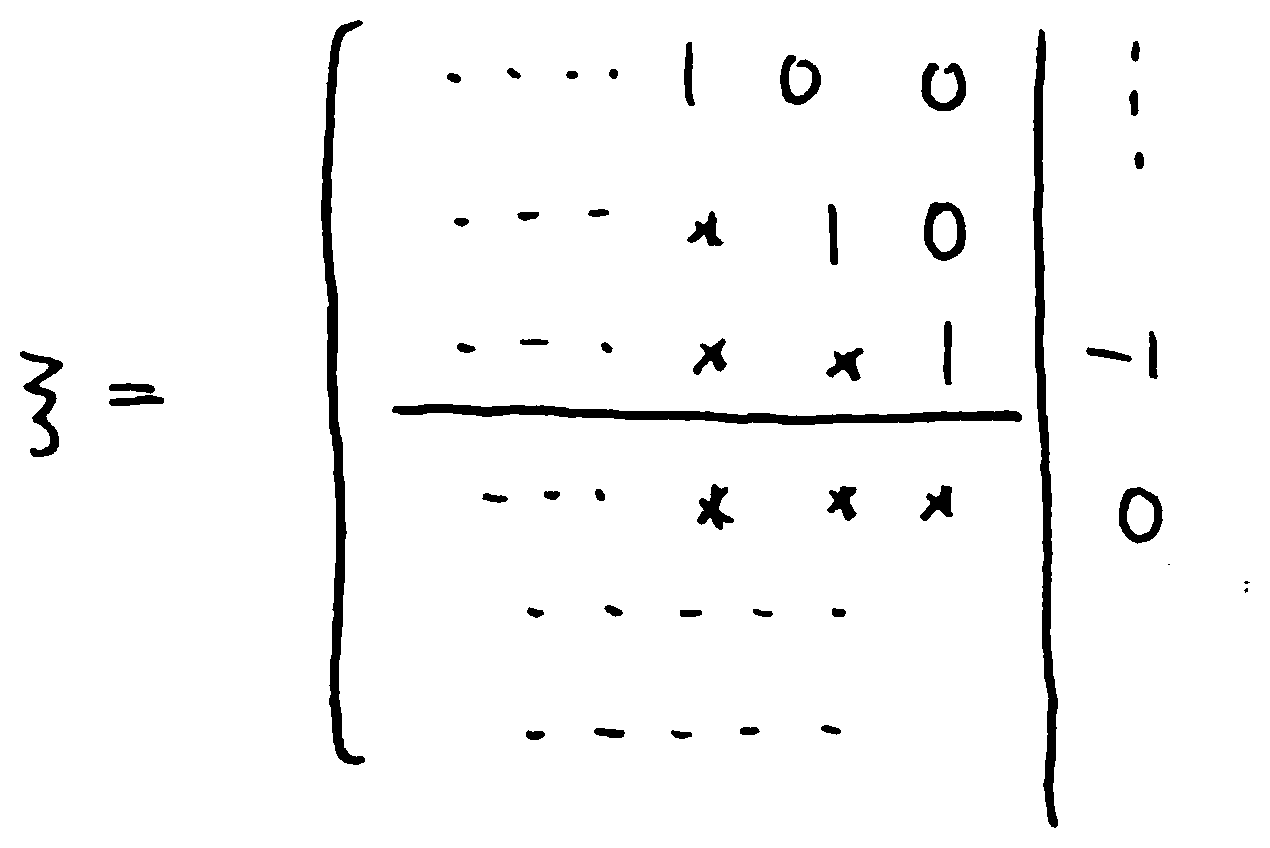
\includegraphics[width=0.55\linewidth]{fig_p89_a.png}
\end{center}
又，与 $Y$ 对应的 index 也只需考虑移动了原点的 Maya 图。Maya 图是指数列 $I=\{\cdots<i_{-3}<i_{-2}<i_{-1}\}$，且对充分大的 $m$ 有 $i_{-m}=-m$。它按下图用图形表示。
\[
\{i_{-4}<i_{-3}<i_{-2}<i_{-1}\}=\{-3,-1,2,4\}
\]
\begin{center}
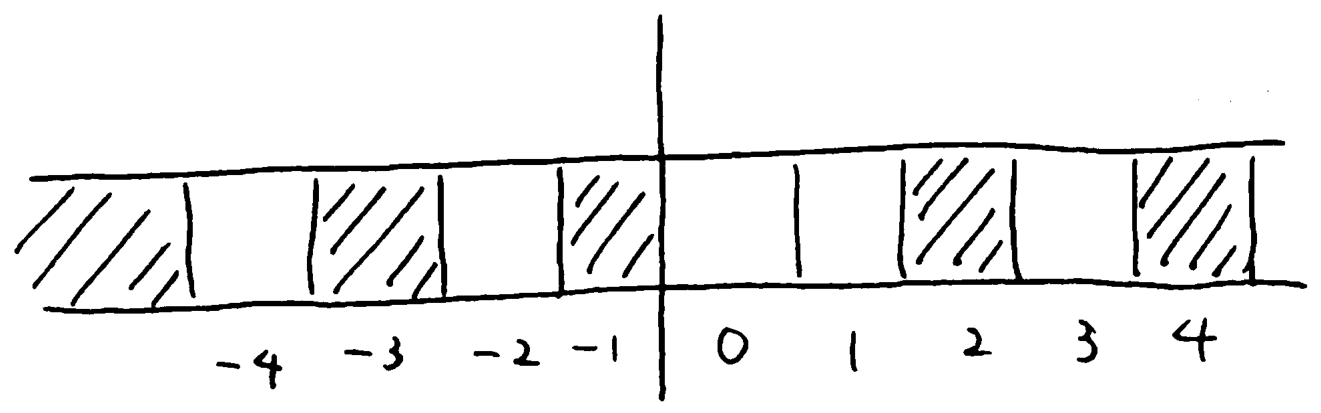
\includegraphics[width=0.78\linewidth]{fig_p89_b.png}
\end{center}
至此便可无碍地把 $\tau$ 函数看作带 frame 的无穷维 Grassmann variety 上的函数。作为 $\C[\partial]$-module，由 $x^n/n!\mapsto\partial^{-n-1}$ 这一对应，有 $\C[[x]]\simeq\C((\partial^{-1}))/\C[\partial]$。给出 $(*)$ 中 $\xi$ 的列向量，就是给出 $f\in\C((\partial^{-1}))$；而给出图 $(*)$ 之形的 $\xi$，等价于给出 $\C((\partial^{-1}))$ 的列 $f_i$ 且满足 $f_i\in\partial^i+\partial^{i-1}\C[[\partial^{-1}]]$（$i=1,2,\dots$）。这里要提醒的是：这样得到的 frame 属于 Grassmann variety 的某个开集，而并非全体。不过绝大多数都属于此，故以下只处理这样的 $\xi$。设 $\{\cdots<i_{-m}<\cdots<i_{-1}\}$ 为 Young diagram $Y$ 对应的 Maya 图，令 $f_i=\sum_j a_{ij}\partial^{-j}$，则 $\xi$ 的 Pluecker 坐
% ===== 原书 p.84 =====
% （本块末：此段起于 p.83，尚余两行在本块；§5.4 起属 c12）
标 $\xi_Y$ 用充分大的 $m$ 表示为
\[
\xi_Y=
\begin{pmatrix}
a_{mi_{-m}} & \cdots & a_{1i_{-m}}\\
\vdots & & \vdots\\
a_{mi_{-1}} & \cdots & a_{1i_{-1}}
\end{pmatrix}
\]
成为如此。此式与充分大的 $m$ 的取法无关。

\transnote{原书此处称「图 $(*)$」，但全书未见标为 $(*)$ 的图（p.82 的 $\xi$ 矩阵、p.83 的 $\xi$ 手绘图均无编号），此处照原文译出，所指待考。}

\transnote{原书正文作 $\xi'=(f'_d,\dots,f'_1)$，紧接的矩阵表示却作 $(f'_{d+1},\dots,f'_1)$，两处不一致，译文照原文排印。}

% c12 —— §5.4 电荷共轭变换与行列式表示；§5.5 Harish-Chandra 定理与 $\tau$ 函数；参考文献
% （原书 p.84–89；p.84 页首两行已由 c11 收尾译完）
% 负责：trans-f

% ===== 原书 p.84 =====
\subsection{电荷共轭变换与行列式表示}

现在，对 $f=f(\partial^{-1})\in\C((\partial^{-1}))$，把 $\partial^{-1}$ 换成 $u$ 所得的 $\C((u))$ 的元素 $f(u)$，称为 $f(\partial^{-1})$ 的电荷共轭变换。（名目上很夸张，实质上几乎什么也没做。）下面用 $\{f_i(u)\}$ 写出 $\tau$ 函数。这里设 $f_i\in u^{-i}+u^{-i+1}\C[[u]]$（$i=1,2,\dots$）。

\begin{lemma}
\[
\tau_m=
\frac{\det
\begin{pmatrix}
f_m(\lambda_1) & \cdots & f_1(\lambda_1)\\
\vdots & & \vdots\\
f_m(\lambda_m) & \cdots & f_1(\lambda_m)
\end{pmatrix}}
{(\lambda_1\cdots\lambda_m)^{-1}\prod_{i<j}(\lambda_i^{-1}-\lambda_j^{-1})}
\]
如此置定时，把 $\tau_m$ 经变换 $t_i=\frac{1}{i}\sum_{j=1}^m\lambda_j^i$ 看作 $t$ 的函数，再用 $t$ 的 Schur 函数 $S_Y$ 展开，则当 $Y$ 的深度不超过 $m$ 时，其系数与 $\xi_Y$ 一致。
\end{lemma}

% ===== 原书 p.85 =====
\begin{proof}
置 $f(u)=\sum_j a_{ij}u^j$。

\transnote{原书此处作 $f(u)$，前文记作 $\{f_i(u)\}$，据上下文疑应为 $f_i(u)$，译文照原文排印。}

\[
\begin{aligned}
\tau_m&=
\frac{\det
\begin{pmatrix}
\lambda_1^m f_m(\lambda_1) & \cdots & \lambda_1^m f_1(\lambda_1)\\
\vdots & & \vdots\\
\lambda_m^m f_m(\lambda_m) & \cdots & \lambda_m^m f_1(\lambda_m)
\end{pmatrix}}
{\prod_{i<j}(\lambda_i-\lambda_j)}\\
&=\det
\begin{pmatrix}
1 & \lambda_1 & \cdots & \lambda_1^m & \cdots\\
\vdots & & & & \vdots\\
1 & \lambda_m & \cdots & \lambda_m^m & \cdots
\end{pmatrix}
\begin{pmatrix}
a_{m,-m} & \cdots & a_{1,-m}\\
\vdots & & \vdots\\
a_{m,0} & \cdots & a_{1,0}
\end{pmatrix}\\
&=\sum_{-m\le i_m<\cdots<i_{-1}}
\frac{\det
\begin{pmatrix}
\lambda_1^{i_{-m}+m} & \cdots & \lambda_1^{i_{-1}+m}\\
\vdots & & \vdots\\
\lambda_m^{i_{-m}+m} & \cdots & \lambda_m^{i_{-1}+m}
\end{pmatrix}}
{\prod_{i<j}(\lambda_i-\lambda_j)}\\
&\qquad\times\det
\begin{pmatrix}
a_{m,i_{-m}} & \cdots & a_{1,i_{-m}}\\
\vdots & & \vdots\\
a_{m,i_{-1}} & \cdots & a_{1,i_{-1}}
\end{pmatrix}
\end{aligned}
\]
成为如此。这里用 Schur 函数的定义
\[
S_Y(t)=
\frac{\det
\begin{pmatrix}
\lambda_1^{i_{-m}+m} & \cdots & \lambda_1^{i_{-1}+m}\\
\vdots & & \vdots\\
\lambda_m^{i_{-m}+m} & \cdots & \lambda_m^{i_{-1}+m}
\end{pmatrix}}
{\prod_{i<j}(\lambda_i-\lambda_j)}
\]
即得引理 5.1。
\end{proof}

\begin{corollary}
引理 5.1 中 $\tau_m$ 的极限 $\lim_{m\to\infty}\tau_m$，作为无限变量对称多项式 $\varprojlim\C[s_i]$（$s_i$ 为基本对称多项式）的元素是良定义的。
\end{corollary}

\subsection{Harish-Chandra 定理与 $\tau$ 函数}

这里用 Harish-Chandra 定理改写矩阵积分。

\begin{theorem}[Harish-Chandra {[HC]}]
设 $Y=\operatorname{diag}(y_i)\in\R^n$ 为对角矩阵，且 $y_i\ne y_j$（$i\ne j$）。设 $\Phi:H_n\to\R$ 为类函数，则存在只依赖于 $n$ 的常数 $c_n$，使
\[
\int_{H_n}\exp(\tr(-\sqrt{-1}YX)\Phi(X)dX
=c_nV(Y)^{-1}\int_{\R^n}\exp(\tr(-\sqrt{-1}YD)\Phi(D)V(D)dD
\]
\end{theorem}

\transnote{上式两处 $\exp($ 在原书中均未闭合，译文照原文排印；通行的写法应补出右括号，作 $\exp(\tr(\cdots))$。}

% ===== 原书 p.86 =====
成为如此。这里对 $Y=\operatorname{diag}(y_i)$，有
\[
V(y)=\prod_{i<j}(y_i-y_j)
\]
用这一定理改写矩阵积分。把 $Y$ 延拓到 $\C$ 上成为全纯函数。又省略积分区域，作形式上的变形。
\[
\Bigl\langle\exp\Bigl(\frac{t\tr(X^3)}{3}\Bigr)\Bigr\rangle
=\int\exp\Bigl(\tr\Bigl(-\frac{1}{2}\Lambda X^2+\frac{tX^3}{3}\Bigr)\Bigr)dX
\]
这里令 $X-\frac{\Lambda}{2t}=Z$ 作积分变量替换，则上式成为
\[
\begin{aligned}
&\Bigl(\int\exp\Bigl(\tr\Bigl(\frac{t}{3}Z^3-\frac{\Lambda^2Z}{4t}\Bigr)\Bigr)dZ\Bigr)\cdot\exp\Bigl(\tr\Bigl(-\frac{\Lambda^3}{12t^2}\Bigr)\Bigr)\\
&=\int\exp\Bigl(\tr\Bigl(\frac{t}{3}Z^3\Bigr)\Bigr)\exp\Bigl(-\tr\frac{\Lambda^2Z}{4t}\Bigr)dZ\cdot\exp\Bigl(\tr\Bigl(-\frac{\Lambda^3}{12t^2}\Bigr)\Bigr)
\end{aligned}
\]
由于 $\exp(\tr(\frac{t}{3}Z^3))$ 是类函数，故用 Harish-Chandra 定理，上式成为
\[
\begin{aligned}
&c_n\frac{1}{\bigl(\frac{-\sqrt{-1}}{4t}\bigr)^{n(n-1)/2}\prod_{i<j}(\lambda_i^2-\lambda_j^2)}\\
&\qquad\times\int V(D)\exp\Bigl(\tr\Bigl(\frac{tD^3}{3}-\frac{\Lambda^2D}{4t}\Bigr)\Bigr)dD\cdot\exp\Bigl(\tr\Bigl(-\frac{\Lambda^3}{12t^2}\Bigr)\Bigr)\\
&=c_n\frac{\exp\bigl(\tr\bigl(-\frac{\Lambda^3}{12t^2}\bigr)\bigr)}{\prod_{i<j}(\lambda_i^2-\lambda_j^2)}
\det\Bigl(\int x^{j-1}\exp\Bigl(\frac{tx^3}{3}-\frac{\lambda_i^2x}{4t}\Bigr)dx\Bigr)_{ij}\\
&=c_n\frac{1}{\prod_{i<j}(\lambda_i^2-\lambda_j^2)}
\det\Bigl(\int\Bigl(x+\frac{\lambda_i}{2t}\Bigr)^{j-1}
\exp\Bigl(-\frac{\lambda_i}{2}x^2+\frac{tx^3}{3}\Bigr)dx\Bigr)_{ij}
\end{aligned}
\]
成为如此。现在令
\[
f_j(x)=\int\Bigl(x+\frac{\lambda}{2t}\Bigr)^{j-1}
\exp\Bigl(-\frac{\lambda}{2}x^2+\frac{t}{3}x^3\Bigr)dx
\]
则上式成为
\[
c'_n\frac{1}{\prod_{i<j}(\lambda_i^2-\lambda_j^2)}\det(f_j(\lambda_j))_{ij}
\]

\transnote{原书此处作 $\det(f_j(\lambda_j))_{ij}$，按上文应为 $\det(f_j(\lambda_i))_{ij}$（即 $\lambda_i^2$ 与 $x+\frac{\lambda_i}{2t}$ 中的 $\lambda_i$），译文照原文排印。}

成为如此。下面看 $f_j(\lambda)$ 关于 $\lambda$ 具有怎样的展开。先展开 $\exp(\frac{t}{3}x^3)$ 的部分来考虑，则只须考虑下面的积分（$1\le k\le j-1$，$m\ge0$）。
\[
\int x^{k+3m}\lambda^{j-k-1}\exp\Bigl(-\frac{\lambda x^2}{2}\Bigr)dx
=c_{j,k,m}\lambda^{-\frac{1}{2}(-2j+3+3m+3k)}
\]

% ===== 原书 p.87 =====
其中 $c_{j,k,m}$ 可看作 $k+3m$ 跑遍 $0$ 以上的偶数。由于
\[
f_j=\lambda^{j-\frac{3}{2}}(a_{j0}+a_{j1}\lambda^{-1}+a_{j2}\lambda^{-2}+\cdots)
\]
具有这种形状，故置
\[
h_j(\lambda^{-1})=\lambda^j(a_{j0}+a_{j1}\lambda^{-1}+a_{j2}\lambda^{-2}+\cdots)
\]
则 $f_j(\lambda)=h_j(\lambda^{-1})\lambda^{-\frac{3}{2}}$。因此
\[
\int\exp\Bigl(-\frac{\Lambda X^2}{2}+\frac{tX^3}{3}\Bigr)dX
=c_n\frac{\prod_{i=1}^n(\lambda_i)^{-\frac{3}{2}}}{\prod_{i<j}(\lambda_i^2-\lambda_j^2)}
\det(h_j(\lambda_i^{-1}))
\]
又
\[
\langle1\rangle=\exp\Bigl(-\frac{\Lambda X^2}{2}\Bigr)dX
=\frac{d_n}{\prod_{i<j}(\lambda_i+\lambda_j)\cdot\prod_{i=1}^n\lambda_i^{\frac{1}{2}}}
\]

\transnote{原书此处作 $\langle1\rangle=\exp\bigl(-\frac{\Lambda X^2}{2}\bigr)dX$，缺积分号（上下文中的 $\langle\exp(\cdot)\rangle$ 均带 $\int$），译文照原文排印。}

（$d_n$ 是只依赖于 $n$ 的常数。）故
\[
\begin{aligned}
\frac{\langle\exp(\frac{t\tr(X^3)}{3})\rangle}{\langle1\rangle}
&=c_n''\frac{\prod_{i<j}(\lambda_i+\lambda_j)\prod(\lambda_i)^{\frac{1}{2}}}
{\prod_{i<j}(\lambda_i^2-\lambda_j^2)\prod(\lambda_i)^{\frac{3}{2}}}\det(h_j(\lambda_i^{-1}))\\
&=c_n''\frac{1}{\prod_{i<j}(\lambda_i-\lambda_j)\prod_{i=1}^n\lambda_i}\det(h_j(\lambda_i^{-1}))
\end{aligned}
\]
成为如此。因此，作变量替换 $\lambda_i^{-1}=\xi_i$、$t_j=\sum_{i=1}^n\xi_i^j/j$，把
\[
\frac{\langle\exp(\frac{t\tr(X^3)}{3})\rangle}{\langle1\rangle}
\]
看作 $(t_1,t_2,\dots)$ 的函数，它便是关于 $(t_1,t_2,\dots)$ 的 $\tau$ 函数。特别地，令 $t=\frac{1}{2}$，则
\[
\frac{\langle\exp(\frac{\tr X^3}{6})\rangle}{\langle1\rangle}
\]
是关于 $(t_1,t_2,\dots)$ 的 $\tau$ 函数。由此得到下述定理。

\begin{theorem}
\[
\exp\Bigl(\Bigl\langle\sum_i T_i\tau_i\Bigr\rangle\Bigr)
=\frac{\langle\exp(\frac{\tr X^3}{6})\rangle}{\langle1\rangle}
\]
经变量替换 $(2d+1)!!T_d=t_{2d+1}$，是 KP 方程的 $\tau$ 函数。
\end{theorem}

\begin{remark}
由此可知 $\frac{\langle\exp(\frac{\tr X^3}{6})\rangle}{\langle1\rangle}$ 只依赖于 $t_{2d+1}$。只依赖于 $t_{2d+1}$ 的 $\tau$ 函数，称为 KdV 方程的 $\tau$ 函数。
% ===== 原书 p.88 =====
一般地，设 $N$ 为自然数，不依赖于变量 $t_{Nk+1}$ 的 $\tau$ 函数，称为 $N$ reduce 型 $\tau$ 函数。作为上述矩阵积分的推广，考虑下面的矩阵积分。（[KS]）
\[
\int_{H_n}\exp\Bigl(\tr\Bigl(-\sqrt{-1}\Bigl(\frac{X^{d+1}}{d+1}-\Lambda X\Bigr)\Bigr)\Bigr)dX
\]
已知其渐近展开是 $N$ reduced 型 $\tau$ 函数，但这一 $\tau$ 函数在模空间意义上的含义至今不明。
\end{remark}

\transnote{原书对同一概念前后分别用 reduce 与 reduced 两种写法，译文分别照原文字面译出，所指相同。}

% ===== 原书 p.89 =====
\addcontentsline{toc}{section}{参考文献}
\section*{参考文献}
\begin{itemize}[leftmargin=2em,itemsep=3pt,topsep=4pt,label={}]
\item {}[HC]:Harish-Chandra, Differentail operators on a semi-simple Lie algebra, Amer.J. Math. 79, pp. 87-120, (1957).
\item {}[KS]:Kac,V., Schwartz, A., Geometric interpretation of the partition function of 2d gravity, Phisical Lett. B257, 329, (1991).
\item {}[L]:Looijenga, E., Intersection theory on Deligne-Mumford compactifications., Asterisque 216, Seminaire Bourbaki, pp. 187-212.
\item {}[Sa]:佐藤幹夫(野海正俊記) ソリトン方程式と普遍グラスマン多様体, 上智大学数学講究録 18.
\item {}[St]:Streble, K., Quadratic differntials, Berlin, Heiderberg, New York, Springer 1984.
\item {}[W]:Witten, E., Two dimensional gravity and intersection theory on moduli space. Surveys in Diff. Geom. 1, pp.243-310.
\end{itemize}

\transnote{原书参考文献照原文抄录，其中若干拼写照原样保留：Differentail（应为 Differential）、Phisical（应为 Physical）、differntials（应为 differentials）、Heiderberg（应为 Heidelberg）、Streble（应为 Strebel）。}


\end{document}
